\documentclass[]{book}
\usepackage{lmodern}
\usepackage{amssymb,amsmath}
\usepackage{ifxetex,ifluatex}
\usepackage{fixltx2e} % provides \textsubscript
\ifnum 0\ifxetex 1\fi\ifluatex 1\fi=0 % if pdftex
  \usepackage[T1]{fontenc}
  \usepackage[utf8]{inputenc}
\else % if luatex or xelatex
  \ifxetex
    \usepackage{mathspec}
  \else
    \usepackage{fontspec}
  \fi
  \defaultfontfeatures{Ligatures=TeX,Scale=MatchLowercase}
\fi
% use upquote if available, for straight quotes in verbatim environments
\IfFileExists{upquote.sty}{\usepackage{upquote}}{}
% use microtype if available
\IfFileExists{microtype.sty}{%
\usepackage{microtype}
\UseMicrotypeSet[protrusion]{basicmath} % disable protrusion for tt fonts
}{}
\usepackage{hyperref}
\hypersetup{unicode=true,
            pdftitle={The Tidynomicon},
            pdfauthor={Greg Wilson},
            pdfborder={0 0 0},
            breaklinks=true}
\urlstyle{same}  % don't use monospace font for urls
\usepackage{natbib}
\bibliographystyle{apalike}
\usepackage{color}
\usepackage{fancyvrb}
\newcommand{\VerbBar}{|}
\newcommand{\VERB}{\Verb[commandchars=\\\{\}]}
\DefineVerbatimEnvironment{Highlighting}{Verbatim}{commandchars=\\\{\}}
% Add ',fontsize=\small' for more characters per line
\usepackage{framed}
\definecolor{shadecolor}{RGB}{248,248,248}
\newenvironment{Shaded}{\begin{snugshade}}{\end{snugshade}}
\newcommand{\AlertTok}[1]{\textcolor[rgb]{0.94,0.16,0.16}{#1}}
\newcommand{\AnnotationTok}[1]{\textcolor[rgb]{0.56,0.35,0.01}{\textbf{\textit{#1}}}}
\newcommand{\AttributeTok}[1]{\textcolor[rgb]{0.77,0.63,0.00}{#1}}
\newcommand{\BaseNTok}[1]{\textcolor[rgb]{0.00,0.00,0.81}{#1}}
\newcommand{\BuiltInTok}[1]{#1}
\newcommand{\CharTok}[1]{\textcolor[rgb]{0.31,0.60,0.02}{#1}}
\newcommand{\CommentTok}[1]{\textcolor[rgb]{0.56,0.35,0.01}{\textit{#1}}}
\newcommand{\CommentVarTok}[1]{\textcolor[rgb]{0.56,0.35,0.01}{\textbf{\textit{#1}}}}
\newcommand{\ConstantTok}[1]{\textcolor[rgb]{0.00,0.00,0.00}{#1}}
\newcommand{\ControlFlowTok}[1]{\textcolor[rgb]{0.13,0.29,0.53}{\textbf{#1}}}
\newcommand{\DataTypeTok}[1]{\textcolor[rgb]{0.13,0.29,0.53}{#1}}
\newcommand{\DecValTok}[1]{\textcolor[rgb]{0.00,0.00,0.81}{#1}}
\newcommand{\DocumentationTok}[1]{\textcolor[rgb]{0.56,0.35,0.01}{\textbf{\textit{#1}}}}
\newcommand{\ErrorTok}[1]{\textcolor[rgb]{0.64,0.00,0.00}{\textbf{#1}}}
\newcommand{\ExtensionTok}[1]{#1}
\newcommand{\FloatTok}[1]{\textcolor[rgb]{0.00,0.00,0.81}{#1}}
\newcommand{\FunctionTok}[1]{\textcolor[rgb]{0.00,0.00,0.00}{#1}}
\newcommand{\ImportTok}[1]{#1}
\newcommand{\InformationTok}[1]{\textcolor[rgb]{0.56,0.35,0.01}{\textbf{\textit{#1}}}}
\newcommand{\KeywordTok}[1]{\textcolor[rgb]{0.13,0.29,0.53}{\textbf{#1}}}
\newcommand{\NormalTok}[1]{#1}
\newcommand{\OperatorTok}[1]{\textcolor[rgb]{0.81,0.36,0.00}{\textbf{#1}}}
\newcommand{\OtherTok}[1]{\textcolor[rgb]{0.56,0.35,0.01}{#1}}
\newcommand{\PreprocessorTok}[1]{\textcolor[rgb]{0.56,0.35,0.01}{\textit{#1}}}
\newcommand{\RegionMarkerTok}[1]{#1}
\newcommand{\SpecialCharTok}[1]{\textcolor[rgb]{0.00,0.00,0.00}{#1}}
\newcommand{\SpecialStringTok}[1]{\textcolor[rgb]{0.31,0.60,0.02}{#1}}
\newcommand{\StringTok}[1]{\textcolor[rgb]{0.31,0.60,0.02}{#1}}
\newcommand{\VariableTok}[1]{\textcolor[rgb]{0.00,0.00,0.00}{#1}}
\newcommand{\VerbatimStringTok}[1]{\textcolor[rgb]{0.31,0.60,0.02}{#1}}
\newcommand{\WarningTok}[1]{\textcolor[rgb]{0.56,0.35,0.01}{\textbf{\textit{#1}}}}
\usepackage{longtable,booktabs}
\usepackage{graphicx,grffile}
\makeatletter
\def\maxwidth{\ifdim\Gin@nat@width>\linewidth\linewidth\else\Gin@nat@width\fi}
\def\maxheight{\ifdim\Gin@nat@height>\textheight\textheight\else\Gin@nat@height\fi}
\makeatother
% Scale images if necessary, so that they will not overflow the page
% margins by default, and it is still possible to overwrite the defaults
% using explicit options in \includegraphics[width, height, ...]{}
\setkeys{Gin}{width=\maxwidth,height=\maxheight,keepaspectratio}
\usepackage[normalem]{ulem}
% avoid problems with \sout in headers with hyperref:
\pdfstringdefDisableCommands{\renewcommand{\sout}{}}
\IfFileExists{parskip.sty}{%
\usepackage{parskip}
}{% else
\setlength{\parindent}{0pt}
\setlength{\parskip}{6pt plus 2pt minus 1pt}
}
\setlength{\emergencystretch}{3em}  % prevent overfull lines
\providecommand{\tightlist}{%
  \setlength{\itemsep}{0pt}\setlength{\parskip}{0pt}}
\setcounter{secnumdepth}{5}
% Redefines (sub)paragraphs to behave more like sections
\ifx\paragraph\undefined\else
\let\oldparagraph\paragraph
\renewcommand{\paragraph}[1]{\oldparagraph{#1}\mbox{}}
\fi
\ifx\subparagraph\undefined\else
\let\oldsubparagraph\subparagraph
\renewcommand{\subparagraph}[1]{\oldsubparagraph{#1}\mbox{}}
\fi

%%% Use protect on footnotes to avoid problems with footnotes in titles
\let\rmarkdownfootnote\footnote%
\def\footnote{\protect\rmarkdownfootnote}

%%% Change title format to be more compact
\usepackage{titling}

% Create subtitle command for use in maketitle
\providecommand{\subtitle}[1]{
  \posttitle{
    \begin{center}\large#1\end{center}
    }
}

\setlength{\droptitle}{-2em}

  \title{The Tidynomicon}
    \pretitle{\vspace{\droptitle}\centering\huge}
  \posttitle{\par}
  \subtitle{A Brief Introduction to R for People Who Count From Zero}
  \author{Greg Wilson}
    \preauthor{\centering\large\emph}
  \postauthor{\par}
    \date{}
    \predate{}\postdate{}
  
\usepackage{booktabs}
\usepackage{amsthm}
\makeatletter
\def\thm@space@setup{%
  \thm@preskip=8pt plus 2pt minus 4pt
  \thm@postskip=\thm@preskip
}
\makeatother
\usepackage{booktabs}
\usepackage{longtable}
\usepackage{array}
\usepackage{multirow}
\usepackage{wrapfig}
\usepackage{float}
\usepackage{colortbl}
\usepackage{pdflscape}
\usepackage{tabu}
\usepackage{threeparttable}
\usepackage{threeparttablex}
\usepackage[normalem]{ulem}
\usepackage{makecell}
\usepackage{xcolor}

\begin{document}
\maketitle

{
\setcounter{tocdepth}{1}
\tableofcontents
}
\hypertarget{introduction}{%
\chapter{Introduction}\label{introduction}}

Years ago,
Patrick Burns wrote \emph{\href{https://www.burns-stat.com/documents/books/the-r-inferno/}{The R Inferno}},
a guide to R for those who think they are in hell.
Upon first encountering the language after two decades of using Python,
I thought Burns was an optimist---after all,
hell has rules.

I have since realized that R does too,
and that they are no more confusing or contradictory than those of other programming languages.
They only appear so because R draws on a tradition unfamiliar to those of us raised with derivatives of C.
Counting from one,
copying data rather than modifying it,
lazy evaluation:
to quote \href{https://www.terrypratchettbooks.com/sir-terry/}{the other bard},
these are not mad, just differently sane.

Welcome, then, to a universe where the strange will become familiar,
and everything familiar, strange.
Welcome, thrice welcome, to R.

\begin{figure}

{\centering 
\includegraphics[width=0.8\linewidth]{figures/index/cthulhu-900x759} 

}

\caption{Speak not of madness, oh you who count from zero.}\label{fig:logo}
\end{figure}

\hypertarget{s:index-personas}{%
\section{Who are these lessons for?}\label{s:index-personas}}

\begin{description}
\tightlist
\item[Andrzej]
completed a Master's in library science five years ago
and has done data analysis for various school boards since then.
He learned Python doing data science courses online,
but has no formal training in programming.
He just joined team that uses R and R~Markdown to generate reports,
and these lessons will show him how to translate his understanding of Python to R.
\item[Padma]
has been building dashboards for a logistics company using Django and D3
while also doing systems administration and managing deployments.
The company has just hired some data scientists
who would like to rebuild some of her dashboards in Shiny.
Padma isn't a statistician,
but would like to learn enough about R to help the analysts
and get their code into production.
\end{description}

\hypertarget{s:index-install}{%
\section{How do I get started?}\label{s:index-install}}

You will learn as much or more from the exercise in this book as from the lessons themselves.
To start,
you can create an account on \href{https://rstudio.cloud/}{rstudio.cloud},
clone \href{https://github.com/gvwilson/tidynomicon/}{the tidynomicon project},
and work in that.
If you prefer to work on your own computer,
you must \href{https://cran.rstudio.com/}{install R} and then \href{https://www.rstudio.com/products/rstudio/download/}{install RStudio}.
We recommend that you do \emph{not} use \href{https://conda.io/}{conda},
\href{https://brew.sh/}{brew},
or other platform-specific package managers to do this,
as they sometimes only install part of what you need.
You will need additional software packages as we go along;
each shall be named and summoned in due course.

\hypertarget{basics}{%
\chapter{Simple Beginnings}\label{basics}}

We begin by introducing the basic elements of R.
You will use these less often than you might expect,
but they are the building blocks for the higher-level tools introduced in Chapter~\ref{tidyverse},
and offer the comfort of familiarity.
Where we feel comparisons would aid understanding,
we provide short examples in Python.

\hypertarget{learning-objectives}{%
\section{Learning Objectives}\label{learning-objectives}}

\begin{itemize}
\tightlist
\item
  Name and describe R's atomic data types and create objects of those types.
\item
  Explain what `scalar' values actually are in R.
\item
  Identify correct and incorrect variable names in R.
\item
  Create vectors in R and index them to select single values, ranges of values, and selected values.
\item
  Explain the difference between \texttt{NA} and \texttt{NULL} and correctly use tests for each.
\item
  Explain the difference between a list and a vector.
\item
  Explain the difference between indexing with \texttt{{[}} and with \texttt{{[}{[}}.
\item
  Use \texttt{{[}} and \texttt{{[}{[}} correctly to extract elements and sub-structures from data structures in R.
\item
  Create a named list in R.
\item
  Access elements by name using both \texttt{{[}} and \texttt{\$} notation.
\item
  Correctly identify cases in which back-quoting is necessary when accessing elements via \texttt{\$}.
\item
  Create and index matrices in R.
\item
  Create \texttt{for} loops and \texttt{if}/\texttt{else} statements in R.
\item
  Explain why vectors cannot be used directly in conditional expressions and correctly use \texttt{all} and \texttt{any} to combine their values.
\item
  Define functions taking a fixed number of named arguments and/or a variable number of arguments.
\item
  Explain what vectorization is and create vectorized equivalents of unnested loops containing simple conditional tests.
\end{itemize}

\hypertarget{how-do-i-say-hello}{%
\section{How do I say hello?}\label{how-do-i-say-hello}}

We begin with a traditional greeting.
In Python, we write:

\begin{Shaded}
\begin{Highlighting}[]
\BuiltInTok{print}\NormalTok{(}\StringTok{"Hello, world!"}\NormalTok{)}
\end{Highlighting}
\end{Shaded}

\begin{verbatim}
Hello, world!
\end{verbatim}

We can run the equivalent R in the RStudio Console (Figure~\ref{fig:console}):

\begin{Shaded}
\begin{Highlighting}[]
\KeywordTok{print}\NormalTok{(}\StringTok{"Hello, world!"}\NormalTok{)}
\end{Highlighting}
\end{Shaded}

\begin{verbatim}
[1] "Hello, world!"
\end{verbatim}

\begin{figure}
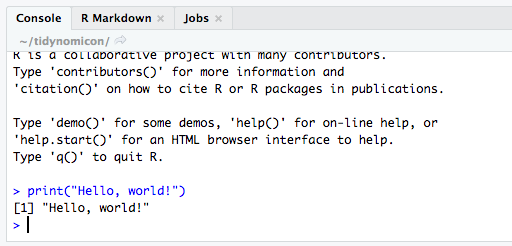
\includegraphics[width=7.11in]{figures/basics/console} \caption{RStudio Console}\label{fig:console}
\end{figure}

Python prints what we asked for,
but what does the \texttt{{[}1{]}} in R's output signify?
Is it perhaps something akin to a line number?
Let's take a closer look by evaluating a couple of expressions without calling \texttt{print}:

\begin{Shaded}
\begin{Highlighting}[]
\StringTok{'This is in single quotes.'}
\end{Highlighting}
\end{Shaded}

\begin{verbatim}
[1] "This is in single quotes."
\end{verbatim}

\begin{Shaded}
\begin{Highlighting}[]
\StringTok{"This is in double quotes."}
\end{Highlighting}
\end{Shaded}

\begin{verbatim}
[1] "This is in double quotes."
\end{verbatim}

\texttt{{[}1{]}} doesn't appear to be a line number;
let's ignore it for now and do a little more exploring.

\begin{quote}
Note that R uses double quotes to display strings even when we give it a single-quoted string
(which is no worse than Python using single quotes when we've given it doubles).
\end{quote}

\hypertarget{how-do-i-add-numbers}{%
\section{How do I add numbers?}\label{how-do-i-add-numbers}}

In Python,
we add numbers using \texttt{+}.

\begin{Shaded}
\begin{Highlighting}[]
\BuiltInTok{print}\NormalTok{(}\DecValTok{1} \OperatorTok{+} \DecValTok{2} \OperatorTok{+} \DecValTok{3}\NormalTok{)}
\end{Highlighting}
\end{Shaded}

\begin{verbatim}
6
\end{verbatim}

We can check the type of the result using \texttt{type},
which tells us that the result \texttt{6} is an integer:

\begin{Shaded}
\begin{Highlighting}[]
\BuiltInTok{print}\NormalTok{(}\BuiltInTok{type}\NormalTok{(}\DecValTok{6}\NormalTok{))}
\end{Highlighting}
\end{Shaded}

\begin{verbatim}
<class 'int'>
\end{verbatim}

What does R do?

\begin{Shaded}
\begin{Highlighting}[]
\DecValTok{1} \OperatorTok{+}\StringTok{ }\DecValTok{2} \OperatorTok{+}\StringTok{ }\DecValTok{3}
\end{Highlighting}
\end{Shaded}

\begin{verbatim}
[1] 6
\end{verbatim}

\begin{Shaded}
\begin{Highlighting}[]
\KeywordTok{typeof}\NormalTok{(}\DecValTok{6}\NormalTok{)}
\end{Highlighting}
\end{Shaded}

\begin{verbatim}
[1] "double"
\end{verbatim}

R's type inspection function is called \texttt{typeof} rather than \texttt{type},
and it returns the type's name as a string.
That's all fine,
but it seems odd for integer addition to produce a double-precision floating-point result.
Let's try an experiment:

\begin{Shaded}
\begin{Highlighting}[]
\KeywordTok{typeof}\NormalTok{(}\DecValTok{6}\NormalTok{)}
\end{Highlighting}
\end{Shaded}

\begin{verbatim}
[1] "double"
\end{verbatim}

Ah: by default,
R represents numbers as floating-point values,
even if they look like integers when written.
We can force a literal value to be an integer by appending an upper-case \texttt{L}
(which stands for ``long integer''):

\begin{Shaded}
\begin{Highlighting}[]
\KeywordTok{typeof}\NormalTok{(6L)}
\end{Highlighting}
\end{Shaded}

\begin{verbatim}
[1] "integer"
\end{verbatim}

Arithmetic on integers does produce integers:

\begin{Shaded}
\begin{Highlighting}[]
\KeywordTok{typeof}\NormalTok{(1L }\OperatorTok{+}\StringTok{ }\NormalTok{2L }\OperatorTok{+}\StringTok{ }\NormalTok{3L)}
\end{Highlighting}
\end{Shaded}

\begin{verbatim}
[1] "integer"
\end{verbatim}

and if we want to convert a floating-point number to an integer we can do so:

\begin{Shaded}
\begin{Highlighting}[]
\KeywordTok{typeof}\NormalTok{(}\KeywordTok{as.integer}\NormalTok{(}\DecValTok{6}\NormalTok{))}
\end{Highlighting}
\end{Shaded}

\begin{verbatim}
[1] "integer"
\end{verbatim}

But wait:
what is that dot in \texttt{as.integer}'s name?
Is there an object called \texttt{as} with a \href{glossary.html\#method}{method} called \texttt{integer}?
The answer is ``no'':
\texttt{.} is (usually) just another character in R;
like the underscore \texttt{\_},
it is used to make names more readable.

\hypertarget{how-do-i-store-many-numbers-together}{%
\section{How do I store many numbers together?}\label{how-do-i-store-many-numbers-together}}

The Elder Gods do not bother to learn most of our names
because there are so many of us and we are so ephemeral.
Similarly, we only give a handful of values in our programs their own names;
we lump the rest together into lists, matrices, and more esoteric structure
so that we too can create, manipulate, and dispose of multitudes with a single imperious command.

The most common such structure in Python is the list.
We create lists using square brackets
and assign a list to a variable using \texttt{=}.
If the variable does not exist, it is created:

\begin{Shaded}
\begin{Highlighting}[]
\NormalTok{primes }\OperatorTok{=}\NormalTok{ [}\DecValTok{3}\NormalTok{, }\DecValTok{5}\NormalTok{, }\DecValTok{7}\NormalTok{, }\DecValTok{11}\NormalTok{]}
\BuiltInTok{print}\NormalTok{(primes)}
\end{Highlighting}
\end{Shaded}

\begin{verbatim}
[3, 5, 7, 11]
\end{verbatim}

Since assignment is a \href{glossary.html\#statement}{statement}
rather than an \href{glossary.html\#expression}{expression},
it has no result,
so Python does not display anything when this command is run.

The equivalent operation in R uses a function called \texttt{c},
which stands for ``column'' and which creates a \href{glossary.html\#vector}{vector}:

\begin{Shaded}
\begin{Highlighting}[]
\NormalTok{primes <-}\StringTok{ }\KeywordTok{c}\NormalTok{(}\DecValTok{3}\NormalTok{, }\DecValTok{5}\NormalTok{, }\DecValTok{7}\NormalTok{, }\DecValTok{11}\NormalTok{)}
\NormalTok{primes}
\end{Highlighting}
\end{Shaded}

\begin{verbatim}
[1]  3  5  7 11
\end{verbatim}

Assignment is done using a left-pointing arrow \texttt{\textless{}-}
(though other forms exist, which we will discuss later).
As in Python,
assignment is a statement rather than an expression,
so we enter the name of the newly-created variable to get R to display its value.

Now that we can create vectors in R,
we can explain the errant \texttt{{[}1{]}} in our previous examples.
To start,
let's have a look at the lengths of various things in Python:

\begin{Shaded}
\begin{Highlighting}[]
\BuiltInTok{print}\NormalTok{(primes, }\BuiltInTok{len}\NormalTok{(primes))}
\end{Highlighting}
\end{Shaded}

\begin{verbatim}
[3, 5, 7, 11] 4
\end{verbatim}

\begin{Shaded}
\begin{Highlighting}[]
\BuiltInTok{print}\NormalTok{(}\BuiltInTok{len}\NormalTok{(}\DecValTok{4}\NormalTok{))}
\end{Highlighting}
\end{Shaded}

\begin{verbatim}
Error in py_call_impl(callable, dots$args, dots$keywords): TypeError: object of type 'int' has no len()

Detailed traceback: 
  File "<string>", line 1, in <module>
\end{verbatim}

Fair enough:
the length of a list is the number of elements it contains,
and since a \href{glossary.html\#scalar}{scalar} like the integer 4 doesn't contain elements,
it has no length.
What of R's vectors?

\begin{Shaded}
\begin{Highlighting}[]
\KeywordTok{length}\NormalTok{(primes)}
\end{Highlighting}
\end{Shaded}

\begin{verbatim}
[1] 4
\end{verbatim}

Good---and numbers?

\begin{Shaded}
\begin{Highlighting}[]
\KeywordTok{length}\NormalTok{(}\DecValTok{4}\NormalTok{)}
\end{Highlighting}
\end{Shaded}

\begin{verbatim}
[1] 1
\end{verbatim}

That's surprising.
Let's have a closer look:

\begin{Shaded}
\begin{Highlighting}[]
\KeywordTok{typeof}\NormalTok{(primes)}
\end{Highlighting}
\end{Shaded}

\begin{verbatim}
[1] "double"
\end{verbatim}

That's also unexpected:
the type of the vector is the type of the elements it contains.
This all becomes clear once we realize that \emph{there are no scalars in R}.
\texttt{4} is not a single lonely integer,
but rather a vector of length one containing the value 4.
When we display its value,
the \texttt{{[}1{]}} that R prints is the index of its first value.
We can prove this by creating and displaying a longer vector:

\begin{Shaded}
\begin{Highlighting}[]
\KeywordTok{c}\NormalTok{(}\DecValTok{1}\NormalTok{, }\DecValTok{2}\NormalTok{, }\DecValTok{3}\NormalTok{, }\DecValTok{4}\NormalTok{, }\DecValTok{5}\NormalTok{, }\DecValTok{6}\NormalTok{, }\DecValTok{7}\NormalTok{, }\DecValTok{8}\NormalTok{, }\DecValTok{9}\NormalTok{, }\DecValTok{10}\NormalTok{, }\DecValTok{1}\NormalTok{, }\DecValTok{2}\NormalTok{, }\DecValTok{3}\NormalTok{, }\DecValTok{4}\NormalTok{, }\DecValTok{5}\NormalTok{, }\DecValTok{6}\NormalTok{, }\DecValTok{7}\NormalTok{, }\DecValTok{8}\NormalTok{, }\DecValTok{9}\NormalTok{, }\DecValTok{10}\NormalTok{,}
  \DecValTok{1}\NormalTok{, }\DecValTok{2}\NormalTok{, }\DecValTok{3}\NormalTok{, }\DecValTok{4}\NormalTok{, }\DecValTok{5}\NormalTok{, }\DecValTok{6}\NormalTok{, }\DecValTok{7}\NormalTok{, }\DecValTok{8}\NormalTok{, }\DecValTok{9}\NormalTok{, }\DecValTok{10}\NormalTok{, }\DecValTok{1}\NormalTok{, }\DecValTok{2}\NormalTok{, }\DecValTok{3}\NormalTok{, }\DecValTok{4}\NormalTok{, }\DecValTok{5}\NormalTok{, }\DecValTok{6}\NormalTok{, }\DecValTok{7}\NormalTok{, }\DecValTok{8}\NormalTok{, }\DecValTok{9}\NormalTok{, }\DecValTok{10}\NormalTok{)}
\end{Highlighting}
\end{Shaded}

\begin{verbatim}
 [1]  1  2  3  4  5  6  7  8  9 10  1  2  3  4  5  6  7  8  9 10  1  2  3
[24]  4  5  6  7  8  9 10  1  2  3  4  5  6  7  8  9 10
\end{verbatim}

In order to help us find out way in our data,
R automatically breaks long lines
and displays the starting index of each line.
These indices also show us that R counts from 1 as humans do,
rather than from zero.
(There are a great many myths about why programming languages do the latter.
\href{http://exple.tive.org/blarg/2013/10/22/citation-needed/}{The truth is stranger than any fiction could be.})

\hypertarget{how-do-i-index-a-vector}{%
\section{How do I index a vector?}\label{how-do-i-index-a-vector}}

Python's rules for indexing are simple once you understand them
(a statement which is also true of quantum mechanics and necromancy).
To avoid confusing indices with values,
let's create a list of color names and index that:

\begin{Shaded}
\begin{Highlighting}[]
\NormalTok{colors }\OperatorTok{=}\NormalTok{ [}\StringTok{"eburnean"}\NormalTok{, }\StringTok{"glaucous"}\NormalTok{, }\StringTok{"wenge"}\NormalTok{]}
\BuiltInTok{print}\NormalTok{(colors[}\DecValTok{0}\NormalTok{])}
\end{Highlighting}
\end{Shaded}

\begin{verbatim}
eburnean
\end{verbatim}

\begin{Shaded}
\begin{Highlighting}[]
\BuiltInTok{print}\NormalTok{(colors[}\DecValTok{2}\NormalTok{])}
\end{Highlighting}
\end{Shaded}

\begin{verbatim}
wenge
\end{verbatim}

\begin{Shaded}
\begin{Highlighting}[]
\NormalTok{colors[}\DecValTok{3}\NormalTok{]}
\end{Highlighting}
\end{Shaded}

\begin{verbatim}
Error in py_call_impl(callable, dots$args, dots$keywords): IndexError: list index out of range

Detailed traceback: 
  File "<string>", line 1, in <module>
\end{verbatim}

\begin{Shaded}
\begin{Highlighting}[]
\BuiltInTok{print}\NormalTok{(colors[}\OperatorTok{-}\DecValTok{1}\NormalTok{])}
\end{Highlighting}
\end{Shaded}

\begin{verbatim}
wenge
\end{verbatim}

Indexing the equivalent vector in R with the indices 1 to 3 produces unsurprising results:

\begin{Shaded}
\begin{Highlighting}[]
\NormalTok{colors <-}\StringTok{ }\KeywordTok{c}\NormalTok{(}\StringTok{"eburnean"}\NormalTok{, }\StringTok{"glaucous"}\NormalTok{, }\StringTok{"wenge"}\NormalTok{)}
\NormalTok{colors[}\DecValTok{1}\NormalTok{]}
\end{Highlighting}
\end{Shaded}

\begin{verbatim}
[1] "eburnean"
\end{verbatim}

\begin{Shaded}
\begin{Highlighting}[]
\NormalTok{colors[}\DecValTok{3}\NormalTok{]}
\end{Highlighting}
\end{Shaded}

\begin{verbatim}
[1] "wenge"
\end{verbatim}

What happens if we go off the end?

\begin{Shaded}
\begin{Highlighting}[]
\NormalTok{colors[}\DecValTok{4}\NormalTok{]}
\end{Highlighting}
\end{Shaded}

\begin{verbatim}
[1] NA
\end{verbatim}

R handles gaps in data using the special value \href{glossary.html\#NA}{\texttt{NA}} (short for ``not available''),
and returns this value when we ask for a nonexistent element of a vector.
But it does more than this---much more.
In Python,
a negative index counts backward from the end of a list.
In R,
we use a negative index to indicate a value that we don't want:

\begin{Shaded}
\begin{Highlighting}[]
\NormalTok{colors[}\OperatorTok{-}\DecValTok{1}\NormalTok{]}
\end{Highlighting}
\end{Shaded}

\begin{verbatim}
[1] "glaucous" "wenge"   
\end{verbatim}

But wait.
If every value in R is a vector,
then when we use 1 or -1 as an index,
we're actually using a vector to index another one.
What happens if the index itself contains more than one value?

\begin{Shaded}
\begin{Highlighting}[]
\NormalTok{colors[}\DecValTok{1}\NormalTok{, }\DecValTok{2}\NormalTok{]}
\end{Highlighting}
\end{Shaded}

\begin{verbatim}
Error in colors[1, 2]: incorrect number of dimensions
\end{verbatim}

That didn't work because R interprets \texttt{{[}i,\ j{]}} as being row and column indices,
and our vector has only one dimension.
What if we create a vector with \texttt{c(...)} and use that as a subscript?

\begin{Shaded}
\begin{Highlighting}[]
\NormalTok{colors[}\KeywordTok{c}\NormalTok{(}\DecValTok{3}\NormalTok{, }\DecValTok{1}\NormalTok{, }\DecValTok{2}\NormalTok{)]}
\end{Highlighting}
\end{Shaded}

\begin{verbatim}
[1] "wenge"    "eburnean" "glaucous"
\end{verbatim}

That works, and allows us to repeat elements:

\begin{Shaded}
\begin{Highlighting}[]
\NormalTok{colors[}\KeywordTok{c}\NormalTok{(}\DecValTok{1}\NormalTok{, }\DecValTok{1}\NormalTok{, }\DecValTok{1}\NormalTok{)]}
\end{Highlighting}
\end{Shaded}

\begin{verbatim}
[1] "eburnean" "eburnean" "eburnean"
\end{verbatim}

Note that this is \href{glossary.html\#pull-indexing}{pull indexing},
i.e.,
the value at location \emph{i} in the index vector specifies which element of the source vector
is being pulled into that location in the result vector (Figure~\ref{fig:pull-indexing}).

\begin{figure}
\centering
\includegraphics{figures/basics/pull-indexing.pdf}
\caption{\label{fig:pull-indexing}Pull Indexing}
\end{figure}

We can also select out several elements:

\begin{Shaded}
\begin{Highlighting}[]
\NormalTok{colors[}\KeywordTok{c}\NormalTok{(}\OperatorTok{-}\DecValTok{1}\NormalTok{, }\DecValTok{-2}\NormalTok{)]}
\end{Highlighting}
\end{Shaded}

\begin{verbatim}
[1] "wenge"
\end{verbatim}

But we cannot simultaneously select elements in (with positive indices) and out (with negative ones):

\begin{Shaded}
\begin{Highlighting}[]
\NormalTok{colors[}\KeywordTok{c}\NormalTok{(}\DecValTok{1}\NormalTok{, }\DecValTok{-1}\NormalTok{)]}
\end{Highlighting}
\end{Shaded}

\begin{verbatim}
Error in colors[c(1, -1)]: only 0's may be mixed with negative subscripts
\end{verbatim}

That error message is suggestive:
what happens if we use 0 as an index?

\begin{Shaded}
\begin{Highlighting}[]
\NormalTok{colors[}\DecValTok{0}\NormalTok{]}
\end{Highlighting}
\end{Shaded}

\begin{verbatim}
character(0)
\end{verbatim}

In order to understand this rather cryptic response,
we can try calling the function \texttt{character} ourselves
with a positive argument:

\begin{Shaded}
\begin{Highlighting}[]
\KeywordTok{character}\NormalTok{(}\DecValTok{3}\NormalTok{)}
\end{Highlighting}
\end{Shaded}

\begin{verbatim}
[1] "" "" ""
\end{verbatim}

Ah:
\texttt{character(N)} constructs a vector of empty strings of the specified length.
The expression \texttt{character(0)} presumably therefore means
``an \href{glossary.html\#empty-vector}{empty vector} of type character''.
From this,
we conclude that the index 0 doesn't correspond to any elements,
so R gives us back something of the right type but with no content.
As a check,
let's try indexing with 0 and 1 together:

\begin{Shaded}
\begin{Highlighting}[]
\NormalTok{colors[}\KeywordTok{c}\NormalTok{(}\DecValTok{0}\NormalTok{, }\DecValTok{1}\NormalTok{)]}
\end{Highlighting}
\end{Shaded}

\begin{verbatim}
[1] "eburnean"
\end{verbatim}

So when 0 is mixed with either positive or negative indices, it is ignored,
which will undoubtedly lead to some puzzling bugs.
What if in-bounds and out-of-bounds indices are mixed?

\begin{Shaded}
\begin{Highlighting}[]
\NormalTok{colors[}\KeywordTok{c}\NormalTok{(}\DecValTok{1}\NormalTok{, }\DecValTok{10}\NormalTok{)]}
\end{Highlighting}
\end{Shaded}

\begin{verbatim}
[1] "eburnean" NA        
\end{verbatim}

That is consistent with the behavior of single indices.

\hypertarget{how-do-i-create-new-vectors-from-old}{%
\section{How do I create new vectors from old?}\label{how-do-i-create-new-vectors-from-old}}

Modern Python encourages programmers to use \href{glossary.html\#list-comprehension}{list comprehensions}
instead of loops,
i.e.,
to write:

\begin{Shaded}
\begin{Highlighting}[]
\NormalTok{original }\OperatorTok{=}\NormalTok{ [}\DecValTok{3}\NormalTok{, }\DecValTok{5}\NormalTok{, }\DecValTok{7}\NormalTok{, }\DecValTok{9}\NormalTok{]}
\NormalTok{doubled }\OperatorTok{=}\NormalTok{ [}\DecValTok{2} \OperatorTok{*}\NormalTok{ x }\ControlFlowTok{for}\NormalTok{ x }\KeywordTok{in}\NormalTok{ original]}
\BuiltInTok{print}\NormalTok{(doubled)}
\end{Highlighting}
\end{Shaded}

\begin{verbatim}
[6, 10, 14, 18]
\end{verbatim}

instead of:

\begin{Shaded}
\begin{Highlighting}[]
\NormalTok{doubled }\OperatorTok{=}\NormalTok{ []}
\ControlFlowTok{for}\NormalTok{ x }\KeywordTok{in}\NormalTok{ original:}
\NormalTok{  doubled.append(}\DecValTok{2} \OperatorTok{*}\NormalTok{ x)}
\BuiltInTok{print}\NormalTok{(doubled)}
\end{Highlighting}
\end{Shaded}

\begin{verbatim}
[6, 10, 14, 18]
\end{verbatim}

If \texttt{original} is a NumPy array, we can shorten this to \texttt{2\ *\ original}.
R provides this capability in the language itself:

\begin{Shaded}
\begin{Highlighting}[]
\NormalTok{original <-}\StringTok{ }\KeywordTok{c}\NormalTok{(}\DecValTok{3}\NormalTok{, }\DecValTok{5}\NormalTok{, }\DecValTok{7}\NormalTok{, }\DecValTok{9}\NormalTok{)}
\NormalTok{doubled <-}\StringTok{ }\DecValTok{2} \OperatorTok{*}\StringTok{ }\NormalTok{original}
\NormalTok{doubled}
\end{Highlighting}
\end{Shaded}

\begin{verbatim}
[1]  6 10 14 18
\end{verbatim}

Modern R strongly encourages us to \href{glossary.html\#vectorize}{vectorize} computations in this way,
i.e.,
to do operations on whole vectors at once rather than looping over their contents.
To aid this,
all arithmetic operations work element by element on vectors:

\begin{Shaded}
\begin{Highlighting}[]
\NormalTok{tens <-}\StringTok{ }\KeywordTok{c}\NormalTok{(}\DecValTok{10}\NormalTok{, }\DecValTok{20}\NormalTok{, }\DecValTok{30}\NormalTok{)}
\NormalTok{hundreds <-}\StringTok{ }\KeywordTok{c}\NormalTok{(}\DecValTok{100}\NormalTok{, }\DecValTok{200}\NormalTok{, }\DecValTok{300}\NormalTok{)}
\NormalTok{tens }\OperatorTok{+}\StringTok{ }\NormalTok{hundreds }\OperatorTok{/}\StringTok{ }\NormalTok{(tens }\OperatorTok{*}\StringTok{ }\NormalTok{hundreds)}
\end{Highlighting}
\end{Shaded}

\begin{verbatim}
[1] 10.10000 20.05000 30.03333
\end{verbatim}

If two vectors of unequal length are used together,
the elements of the shorter are \href{glossary.html\#recycle}{recycled}.
This behaves sensibly if one of the vectors is a scalar---it is just re-used as many times as necessary:

\begin{Shaded}
\begin{Highlighting}[]
\NormalTok{hundreds }\OperatorTok{+}\StringTok{ }\DecValTok{5}
\end{Highlighting}
\end{Shaded}

\begin{verbatim}
[1] 105 205 305
\end{verbatim}

If both vectors have several elements,
the shorter is repeated as often as necessary.
This works,
but is so likely to lead to hard-to-find bugs that R produces a warning message:

\begin{Shaded}
\begin{Highlighting}[]
\NormalTok{thousands <-}\StringTok{ }\KeywordTok{c}\NormalTok{(}\DecValTok{1000}\NormalTok{, }\DecValTok{2000}\NormalTok{)}
\NormalTok{hundreds }\OperatorTok{+}\StringTok{ }\NormalTok{thousands}
\end{Highlighting}
\end{Shaded}

\begin{verbatim}
Warning in hundreds + thousands: longer object length is not a multiple of
shorter object length
\end{verbatim}

\begin{verbatim}
[1] 1100 2200 1300
\end{verbatim}

R also provides vectorized alternatives to \texttt{if}-\texttt{else} statements.
If we use a vector containing the logical (or Boolean) values \texttt{TRUE} and \texttt{FALSE} as an index,
it selects elements corresponding to \texttt{TRUE} values:

\begin{Shaded}
\begin{Highlighting}[]
\NormalTok{colors }\CommentTok{# as a reminder}
\end{Highlighting}
\end{Shaded}

\begin{verbatim}
[1] "eburnean" "glaucous" "wenge"   
\end{verbatim}

\begin{Shaded}
\begin{Highlighting}[]
\NormalTok{colors[}\KeywordTok{c}\NormalTok{(}\OtherTok{TRUE}\NormalTok{, }\OtherTok{FALSE}\NormalTok{, }\OtherTok{TRUE}\NormalTok{)]}
\end{Highlighting}
\end{Shaded}

\begin{verbatim}
[1] "eburnean" "wenge"   
\end{verbatim}

This is called \href{glossary.html\#logical-indexing}{logical indexing},
though to the best of my knowledge illogical indexing is not provided as an alternative.
The function \texttt{ifelse} uses this to do what its name suggests:
select a value from one vector if a condition is \texttt{TRUE},
and a corresponding value from another vector if the condition is \texttt{FALSE}:

\begin{Shaded}
\begin{Highlighting}[]
\NormalTok{before_letter_m <-}\StringTok{ }\NormalTok{colors }\OperatorTok{<}\StringTok{ "m"}
\NormalTok{before_letter_m }\CommentTok{# to show the index}
\end{Highlighting}
\end{Shaded}

\begin{verbatim}
[1]  TRUE  TRUE FALSE
\end{verbatim}

\begin{Shaded}
\begin{Highlighting}[]
\KeywordTok{ifelse}\NormalTok{(before_letter_m, colors, }\KeywordTok{c}\NormalTok{(}\StringTok{"comes"}\NormalTok{, }\StringTok{"after"}\NormalTok{, }\StringTok{"m"}\NormalTok{))}
\end{Highlighting}
\end{Shaded}

\begin{verbatim}
[1] "eburnean" "glaucous" "m"       
\end{verbatim}

All three vectors are of the same length,
and the first (the condition) is usually constructed using the values of one or both of the other vectors:

\begin{Shaded}
\begin{Highlighting}[]
\KeywordTok{ifelse}\NormalTok{(colors }\OperatorTok{<}\StringTok{ "m"}\NormalTok{, colors, }\KeywordTok{toupper}\NormalTok{(colors))}
\end{Highlighting}
\end{Shaded}

\begin{verbatim}
[1] "eburnean" "glaucous" "WENGE"   
\end{verbatim}

\begin{figure}
\centering
\includegraphics{figures/basics/if-else.pdf}
\caption{\label{fig:ifelse-fig}Vector Conditionals}
\end{figure}

\hypertarget{how-else-does-r-represent-the-absence-of-data}{%
\section{How else does R represent the absence of data?}\label{how-else-does-r-represent-the-absence-of-data}}

The special value \texttt{NA} means ``there's supposed to be a value here but we don't know what it is.''
A different value, \href{glossary.html\#null}{\texttt{NULL}}, represents the absence of a vector.
It is not the same as a vector of zero length,
though testing that statement produces a rather odd result:

\begin{Shaded}
\begin{Highlighting}[]
\OtherTok{NULL} \OperatorTok{==}\StringTok{ }\KeywordTok{integer}\NormalTok{(}\DecValTok{0}\NormalTok{)}
\end{Highlighting}
\end{Shaded}

\begin{verbatim}
logical(0)
\end{verbatim}

The safe way to test if something is \texttt{NULL} is to use the function \texttt{is.null}:

\begin{Shaded}
\begin{Highlighting}[]
\KeywordTok{is.null}\NormalTok{(}\OtherTok{NULL}\NormalTok{)}
\end{Highlighting}
\end{Shaded}

\begin{verbatim}
[1] TRUE
\end{verbatim}

Circling back,
the safe way to test whether a value is \texttt{NA} is \emph{not} to use direct comparison:

\begin{Shaded}
\begin{Highlighting}[]
\NormalTok{threshold <-}\StringTok{ }\FloatTok{1.75}
\NormalTok{threshold }\OperatorTok{==}\StringTok{ }\OtherTok{NA}
\end{Highlighting}
\end{Shaded}

\begin{verbatim}
[1] NA
\end{verbatim}

The result is \texttt{NA} because if we don't know what the value is,
we can't know if it's equal to \texttt{threshold} or not.
Instead,
we should always use the function \texttt{is.na}:

\begin{Shaded}
\begin{Highlighting}[]
\KeywordTok{is.na}\NormalTok{(threshold)}
\end{Highlighting}
\end{Shaded}

\begin{verbatim}
[1] FALSE
\end{verbatim}

\begin{Shaded}
\begin{Highlighting}[]
\KeywordTok{is.na}\NormalTok{(}\OtherTok{NA}\NormalTok{)}
\end{Highlighting}
\end{Shaded}

\begin{verbatim}
[1] TRUE
\end{verbatim}

\hypertarget{how-can-i-store-a-mix-of-different-types-of-objects}{%
\section{How can I store a mix of different types of objects?}\label{how-can-i-store-a-mix-of-different-types-of-objects}}

One of the things that newcomers to R often trip over is the various ways in which structures can be indexed.
All of the following are legal:

\begin{Shaded}
\begin{Highlighting}[]
\NormalTok{thing[i]}
\NormalTok{thing[i, j]}
\NormalTok{thing[[i]]}
\NormalTok{thing[[i, j]]}
\NormalTok{thing}\OperatorTok{$}\NormalTok{name}
\NormalTok{thing}\OperatorTok{$}\StringTok{"name"}
\end{Highlighting}
\end{Shaded}

but they can behave differently depending on what kind of thing \texttt{thing} is.
To explain, we must first take a look at lists.

A \href{glossary.html\#list}{list} in R is a vector that can contain values of many different types.
(The technical term for this is \href{glossary.html\#heterogeneous}{heterogeneous},
in contrast with a \href{glossary.html\#homogeneous}{homogeneous} data structure
that can only contain one type of value.)
We'll use this list in our examples:

\begin{Shaded}
\begin{Highlighting}[]
\NormalTok{thing <-}\StringTok{ }\KeywordTok{list}\NormalTok{(}\StringTok{"first"}\NormalTok{, }\KeywordTok{c}\NormalTok{(}\DecValTok{2}\NormalTok{, }\DecValTok{20}\NormalTok{, }\DecValTok{200}\NormalTok{), }\FloatTok{3.3}\NormalTok{)}
\NormalTok{thing}
\end{Highlighting}
\end{Shaded}

\begin{verbatim}
[[1]]
[1] "first"

[[2]]
[1]   2  20 200

[[3]]
[1] 3.3
\end{verbatim}

The output tells us that the first element of \texttt{thing} is a vector of one element,
that the second is a vector of three elements,
and the third is again a vector of one element;
the major indices are shown in \texttt{{[}{[}\ldots{}{]}{]}},
while the indices of the contained elements are shown in \texttt{{[}\ldots{}{]}}.
(Again,
remember that \texttt{"first"} and 3.3 are actually vectors of length 1.)

\begin{quote}
In keeping with R's conventions,
we will henceforth use \texttt{{[}{[}} and \texttt{{[}} to refer to the two kinds of indexing
rather than \texttt{{[}{[}\ldots{}{]}{]}} and \texttt{{[}\ldots{}{]}}.
\end{quote}

\hypertarget{what-is-the-difference-between-and}{%
\section{\texorpdfstring{What is the difference between \texttt{{[}} and \texttt{{[}{[}}?}{What is the difference between {[} and {[}{[}?}}\label{what-is-the-difference-between-and}}

The output above strongly suggests that we can get the elements of a list using \texttt{{[}{[}} (double square brackets):

\begin{Shaded}
\begin{Highlighting}[]
\NormalTok{thing[[}\DecValTok{1}\NormalTok{]]}
\end{Highlighting}
\end{Shaded}

\begin{verbatim}
[1] "first"
\end{verbatim}

\begin{Shaded}
\begin{Highlighting}[]
\NormalTok{thing[[}\DecValTok{2}\NormalTok{]]}
\end{Highlighting}
\end{Shaded}

\begin{verbatim}
[1]   2  20 200
\end{verbatim}

\begin{Shaded}
\begin{Highlighting}[]
\NormalTok{thing[[}\DecValTok{3}\NormalTok{]]}
\end{Highlighting}
\end{Shaded}

\begin{verbatim}
[1] 3.3
\end{verbatim}

Let's have a look at the types of those three values:

\begin{Shaded}
\begin{Highlighting}[]
\KeywordTok{typeof}\NormalTok{(thing[[}\DecValTok{1}\NormalTok{]])}
\end{Highlighting}
\end{Shaded}

\begin{verbatim}
[1] "character"
\end{verbatim}

\begin{Shaded}
\begin{Highlighting}[]
\KeywordTok{typeof}\NormalTok{(thing[[}\DecValTok{2}\NormalTok{]])}
\end{Highlighting}
\end{Shaded}

\begin{verbatim}
[1] "double"
\end{verbatim}

\begin{Shaded}
\begin{Highlighting}[]
\KeywordTok{typeof}\NormalTok{(thing[[}\DecValTok{3}\NormalTok{]])}
\end{Highlighting}
\end{Shaded}

\begin{verbatim}
[1] "double"
\end{verbatim}

That seems sensible.
Now,
what do we get if we index single square brackets \texttt{{[}\ldots{}{]}}?

\begin{Shaded}
\begin{Highlighting}[]
\NormalTok{thing[}\DecValTok{1}\NormalTok{]}
\end{Highlighting}
\end{Shaded}

\begin{verbatim}
[[1]]
[1] "first"
\end{verbatim}

That looks like a list, not a vector---let's check:

\begin{Shaded}
\begin{Highlighting}[]
\KeywordTok{typeof}\NormalTok{(thing[}\DecValTok{1}\NormalTok{])}
\end{Highlighting}
\end{Shaded}

\begin{verbatim}
[1] "list"
\end{verbatim}

This shows the difference between \texttt{{[}{[}} and \texttt{{[}}:
the former peels away a layer of data structure, returning only the sub-structure,
while the latter gives us back a structure of the same type as the thing being indexed.
Since a ``scalar'' is just a vector of length 1,
there is no difference between \texttt{{[}{[}} and \texttt{{[}} when they are applied to vectors:

\begin{Shaded}
\begin{Highlighting}[]
\NormalTok{v <-}\StringTok{ }\KeywordTok{c}\NormalTok{(}\StringTok{"first"}\NormalTok{, }\StringTok{"second"}\NormalTok{, }\StringTok{"third"}\NormalTok{)}
\NormalTok{v[}\DecValTok{2}\NormalTok{]}
\end{Highlighting}
\end{Shaded}

\begin{verbatim}
[1] "second"
\end{verbatim}

\begin{Shaded}
\begin{Highlighting}[]
\KeywordTok{typeof}\NormalTok{(v[}\DecValTok{2}\NormalTok{])}
\end{Highlighting}
\end{Shaded}

\begin{verbatim}
[1] "character"
\end{verbatim}

\begin{Shaded}
\begin{Highlighting}[]
\NormalTok{v[[}\DecValTok{2}\NormalTok{]]}
\end{Highlighting}
\end{Shaded}

\begin{verbatim}
[1] "second"
\end{verbatim}

\begin{Shaded}
\begin{Highlighting}[]
\KeywordTok{typeof}\NormalTok{(v[[}\DecValTok{2}\NormalTok{]])}
\end{Highlighting}
\end{Shaded}

\begin{verbatim}
[1] "character"
\end{verbatim}

\begin{quote}
\textbf{Flattening and Recursive Indexing}

If a list is just a vector of objects, why do we need the function \texttt{list}?
Why can't we create a list with \texttt{c("first",\ c(2,\ 20,\ 200),\ 30)}?
The answer is that R flattens the arguments to \texttt{c},
so that \texttt{c(c(1,\ 2),\ c(3,\ 4))} produces \texttt{c(1,\ 2,\ 3,\ 4)}.
It also does automatic type conversion:
\texttt{c("first",\ c(2,\ 20,\ 200),\ 30)} produces a vector of character strings
\texttt{c("first",\ "2",\ "20",\ "200",\ "30")}.
This is helpful once you get used to it
(which once again is true of both quantum mechanics and necromancy).

Another ``helpful, ish'' behavior is that using \texttt{{[}{[}} with a list subsets recursively:
if \texttt{thing\ \textless{}-\ list(a\ =\ list(b\ =\ list(c\ =\ list(d\ =\ 1))))},
then \texttt{thing{[}{[}c("a",\ "b",\ "c",\ "d"){]}{]}} selects the 1.
\end{quote}

\hypertarget{how-can-i-access-elements-by-name}{%
\section{How can I access elements by name?}\label{how-can-i-access-elements-by-name}}

R allows us to name the elements in vectors and lists:
if we assign \texttt{c(one\ =\ 1,\ two\ =\ 2,\ three\ =\ 3)} to \texttt{names},
then \texttt{names{[}"two"{]}} is 2.
We can use this to create a lookup table:

\begin{Shaded}
\begin{Highlighting}[]
\NormalTok{values <-}\StringTok{ }\KeywordTok{c}\NormalTok{(}\StringTok{"m"}\NormalTok{, }\StringTok{"f"}\NormalTok{, }\StringTok{"nb"}\NormalTok{, }\StringTok{"f"}\NormalTok{, }\StringTok{"f"}\NormalTok{, }\StringTok{"m"}\NormalTok{, }\StringTok{"m"}\NormalTok{)}
\NormalTok{lookup <-}\StringTok{ }\KeywordTok{c}\NormalTok{(}\DataTypeTok{m =} \StringTok{"Male"}\NormalTok{, }\DataTypeTok{f =} \StringTok{"Female"}\NormalTok{, }\DataTypeTok{nb =} \StringTok{"Non-binary"}\NormalTok{)}
\NormalTok{lookup[values]}
\end{Highlighting}
\end{Shaded}

\begin{verbatim}
           m            f           nb            f            f 
      "Male"     "Female" "Non-binary"     "Female"     "Female" 
           m            m 
      "Male"       "Male" 
\end{verbatim}

If the structure in question is a list rather than an atomic vector of numbers, characters, or logicals,
we can use the syntax \texttt{lookup\$m} instead of \texttt{lookup{[}"m"{]}}:

\begin{Shaded}
\begin{Highlighting}[]
\NormalTok{lookup_list <-}\StringTok{ }\KeywordTok{list}\NormalTok{(}\DataTypeTok{m =} \StringTok{"Male"}\NormalTok{, }\DataTypeTok{f =} \StringTok{"Female"}\NormalTok{, }\DataTypeTok{nb =} \StringTok{"Non-binary"}\NormalTok{)}
\NormalTok{lookup_list}\OperatorTok{$}\NormalTok{m}
\end{Highlighting}
\end{Shaded}

\begin{verbatim}
[1] "Male"
\end{verbatim}

We will explore this in more detail when we look at the tidyverse in Chapter~\ref{tidyverse},
since that is where access-by-name is used most often.
For now,
simply note that if the name of an element isn't a legal variable name,
we have to put it in backward quotes to use it with \texttt{\$}:

\begin{Shaded}
\begin{Highlighting}[]
\NormalTok{another_list <-}\StringTok{ }\KeywordTok{list}\NormalTok{(}\StringTok{"first field"}\NormalTok{ =}\StringTok{ "F"}\NormalTok{, }\StringTok{"second field"}\NormalTok{ =}\StringTok{ "S"}\NormalTok{)}
\NormalTok{another_list}\OperatorTok{$}\StringTok{`}\DataTypeTok{first field}\StringTok{`}
\end{Highlighting}
\end{Shaded}

\begin{verbatim}
[1] "F"
\end{verbatim}

\begin{quote}
If you have control,
or at least the illusion thereof,
choose names such as \texttt{first\_field} that don't require back-quoting.
\end{quote}

\hypertarget{how-can-i-create-and-index-a-matrix}{%
\section{How can I create and index a matrix?}\label{how-can-i-create-and-index-a-matrix}}

Matrices are frequently used in statistics, so R provides built-in support for them.
After \texttt{a\ \textless{}-\ matrix(1:9,\ nrow\ =\ 3)},
\texttt{a} is a 3x3 matrix containing the values 1 through 9:

\begin{Shaded}
\begin{Highlighting}[]
\NormalTok{a <-}\StringTok{ }\KeywordTok{matrix}\NormalTok{(}\DecValTok{1}\OperatorTok{:}\DecValTok{9}\NormalTok{, }\DataTypeTok{nrow =} \DecValTok{3}\NormalTok{)}
\NormalTok{a}
\end{Highlighting}
\end{Shaded}

\begin{verbatim}
     [,1] [,2] [,3]
[1,]    1    4    7
[2,]    2    5    8
[3,]    3    6    9
\end{verbatim}

Behind the scenes,
a matrix is a vector with an \href{glossary.html\#attribute}{attribute} called \texttt{dim} that stores its dimensions:

\begin{Shaded}
\begin{Highlighting}[]
\KeywordTok{dim}\NormalTok{(a)}
\end{Highlighting}
\end{Shaded}

\begin{verbatim}
[1] 3 3
\end{verbatim}

\texttt{a{[}3,\ 3{]}} is a vector of length 1 containing the value 9 (again, ``scalars'' in R are actually vectors),
while \texttt{a{[}1,{]}} is the vector \texttt{c(1,\ 4,\ 7)} (because we are selecting the first row of the matrix)
and \texttt{a{[},1{]}} is the vector \texttt{c(1,\ 2,\ 3)} (because we are selecting the first column of the matrix).
Elements can still be accessed using a single index,
which returns the value from that location in the underlying vector:

\begin{Shaded}
\begin{Highlighting}[]
\NormalTok{a[}\DecValTok{8}\NormalTok{]}
\end{Highlighting}
\end{Shaded}

\begin{verbatim}
[1] 8
\end{verbatim}

\hypertarget{how-do-i-choose-and-repeat-things}{%
\section{How do I choose and repeat things?}\label{how-do-i-choose-and-repeat-things}}

We cherish the illusion of free will so much that we embed a pretense of it in our machines
in the form of conditional statements using \texttt{if} and \texttt{else}.
(Ironically,
we then instruct those same machines to make the same decisions over and over.
It's no wonder they sometimes appear mad\ldots{})
For example,
here is a snippet of Python that uses \texttt{for} and \texttt{if} to display
the signs of the numbers in a list:

\begin{Shaded}
\begin{Highlighting}[]
\NormalTok{values }\OperatorTok{=}\NormalTok{ [}\OperatorTok{-}\DecValTok{15}\NormalTok{, }\DecValTok{0}\NormalTok{, }\DecValTok{15}\NormalTok{]}
\ControlFlowTok{for}\NormalTok{ v }\KeywordTok{in}\NormalTok{ values:}
    \ControlFlowTok{if}\NormalTok{ v }\OperatorTok{<} \DecValTok{0}\NormalTok{:}
\NormalTok{        pos_neg }\OperatorTok{=} \DecValTok{-1}
    \ControlFlowTok{elif}\NormalTok{ v }\OperatorTok{==} \DecValTok{0}\NormalTok{:}
\NormalTok{        pos_neg }\OperatorTok{=} \DecValTok{0}
    \ControlFlowTok{else}\NormalTok{:}
\NormalTok{        pos_neg }\OperatorTok{=} \DecValTok{1}
    \BuiltInTok{print}\NormalTok{(}\StringTok{"The pos_neg of"}\NormalTok{, v, }\StringTok{"is"}\NormalTok{, pos_neg)}
\end{Highlighting}
\end{Shaded}

\begin{verbatim}
The pos_neg of -15 is -1
The pos_neg of 0 is 0
The pos_neg of 15 is 1
\end{verbatim}

\begin{Shaded}
\begin{Highlighting}[]
\BuiltInTok{print}\NormalTok{(}\StringTok{"The final value of v is"}\NormalTok{, v)}
\end{Highlighting}
\end{Shaded}

\begin{verbatim}
The final value of v is 15
\end{verbatim}

Its direct translation into R is:

\begin{Shaded}
\begin{Highlighting}[]
\NormalTok{values <-}\StringTok{ }\KeywordTok{c}\NormalTok{(}\OperatorTok{-}\DecValTok{15}\NormalTok{, }\DecValTok{0}\NormalTok{, }\DecValTok{15}\NormalTok{)}
\ControlFlowTok{for}\NormalTok{ (v }\ControlFlowTok{in}\NormalTok{ values) \{}
  \ControlFlowTok{if}\NormalTok{ (v }\OperatorTok{<}\StringTok{ }\DecValTok{0}\NormalTok{) \{}
\NormalTok{    pos_neg <-}\StringTok{ }\DecValTok{-1}
\NormalTok{  \}}
  \ControlFlowTok{else} \ControlFlowTok{if}\NormalTok{ (v }\OperatorTok{==}\StringTok{ }\DecValTok{0}\NormalTok{) \{}
\NormalTok{    pos_neg <-}\StringTok{ }\DecValTok{0}
\NormalTok{  \}}
  \ControlFlowTok{else}\NormalTok{ \{}
\NormalTok{    pos_neg <-}\StringTok{ }\DecValTok{1}
\NormalTok{  \}}
  \KeywordTok{print}\NormalTok{(glue}\OperatorTok{::}\KeywordTok{glue}\NormalTok{(}\StringTok{"The sign of \{v\} is \{pos_neg\}"}\NormalTok{))}
\NormalTok{\}}
\end{Highlighting}
\end{Shaded}

\begin{verbatim}
The sign of -15 is -1
The sign of 0 is 0
The sign of 15 is 1
\end{verbatim}

\begin{Shaded}
\begin{Highlighting}[]
\KeywordTok{print}\NormalTok{(glue}\OperatorTok{::}\KeywordTok{glue}\NormalTok{(}\StringTok{"The final value of v is \{v\}"}\NormalTok{))}
\end{Highlighting}
\end{Shaded}

\begin{verbatim}
The final value of v is 15
\end{verbatim}

There are a few things to note here:

\begin{enumerate}
\def\labelenumi{\arabic{enumi}.}
\tightlist
\item
  The parentheses in the loop header are required:
  we cannot simply write \texttt{for\ v\ in\ values}.
\item
  The curly braces around the body of the loop
  and around the bodies of the conditional branches are optional,
  since each contains only a single statement.
  However, they should always be there to help readability.
\item
  As in Python,
  the loop variable \texttt{v} persists after the loop is over.
\item
  \texttt{glue::glue} (the function \texttt{glue} from the library of the same name)
  interpolates variables into strings in sensible ways.
  We will load this library and use plain old \texttt{glue} in the explanations that follow.
  (Note that R uses \texttt{::} to get functions out of packages rather than Python's \texttt{.}.)
\item
  We have called our temporary variable \texttt{pos\_neg} rather than \texttt{sign}
  so that we don't accidentally overwrite the rather useful built-in R function
  with the latter name.
  \href{glossary.html\#name-collision}{Name collisions} of this sort
  are just as easy in R as they are in Python.
\end{enumerate}

\hypertarget{how-can-i-vectorize-loops-and-conditionals}{%
\section{How can I vectorize loops and conditionals?}\label{how-can-i-vectorize-loops-and-conditionals}}

The example above is \emph{not} how we should write R:
everything in that snippet can and should be vectorized.
The simplest way to do this is to use the aforementioned built-in function:

\begin{Shaded}
\begin{Highlighting}[]
\KeywordTok{print}\NormalTok{(}\KeywordTok{sign}\NormalTok{(values))}
\end{Highlighting}
\end{Shaded}

\begin{verbatim}
[1] -1  0  1
\end{verbatim}

\begin{Shaded}
\begin{Highlighting}[]
\KeywordTok{print}\NormalTok{(glue}\OperatorTok{::}\KeywordTok{glue}\NormalTok{(}\StringTok{"The sign of \{values\} is \{sign(values)\}"}\NormalTok{))}
\end{Highlighting}
\end{Shaded}

\begin{verbatim}
The sign of -15 is -1
The sign of 0 is 0
The sign of 15 is 1
\end{verbatim}

But what if the function we want doesn't exist
(or if we don't know what it's called)?
In that case,
the easiest approach is often to create a new vector
whose values are derived from those of the vector we had
and trust R to match up corresponding elements:

\begin{Shaded}
\begin{Highlighting}[]
\NormalTok{pos_neg <-}\StringTok{ }\NormalTok{dplyr}\OperatorTok{::}\KeywordTok{case_when}\NormalTok{(}
\NormalTok{  values }\OperatorTok{<}\StringTok{  }\DecValTok{0} \OperatorTok{~}\StringTok{ }\DecValTok{-1}\NormalTok{,}
\NormalTok{  values }\OperatorTok{==}\StringTok{ }\DecValTok{0} \OperatorTok{~}\StringTok{ }\DecValTok{0}\NormalTok{,}
\NormalTok{  values }\OperatorTok{>}\StringTok{  }\DecValTok{0} \OperatorTok{~}\StringTok{ }\DecValTok{1}
\NormalTok{)}

\KeywordTok{print}\NormalTok{(glue}\OperatorTok{::}\KeywordTok{glue}\NormalTok{(}\StringTok{"The sign of \{values\} is \{pos_neg\}"}\NormalTok{))}
\end{Highlighting}
\end{Shaded}

\begin{verbatim}
The sign of -15 is -1
The sign of 0 is 0
The sign of 15 is 1
\end{verbatim}

This solution makes use of \texttt{case\_when},
which is a vectorized analog of \texttt{if}/\texttt{else~if}/\texttt{else}.
Each branch uses the \texttt{\textasciitilde{}} operator to combine
a Boolean test on the left with a result on the right.
We will see other uses for \texttt{\textasciitilde{}} in subsequent chapters.

\hypertarget{how-can-i-express-a-range-of-values}{%
\section{How can I express a range of values?}\label{how-can-i-express-a-range-of-values}}

\texttt{for} in R loops over the values in a vector, just as it does in Python.
If we want to loop over the indices instead,
we can use the function \texttt{seq\_along}:

\begin{Shaded}
\begin{Highlighting}[]
\NormalTok{colors <-}\StringTok{ }\KeywordTok{c}\NormalTok{(}\StringTok{"eburnean"}\NormalTok{, }\StringTok{"glaucous"}\NormalTok{, }\StringTok{"squamous"}\NormalTok{, }\StringTok{"wenge"}\NormalTok{)}
\ControlFlowTok{for}\NormalTok{ (i }\ControlFlowTok{in} \KeywordTok{seq_along}\NormalTok{(colors)) \{}
  \KeywordTok{print}\NormalTok{(}\KeywordTok{glue}\NormalTok{(}\StringTok{"The length of color \{i\} is \{length(colors[i])\}"}\NormalTok{))}
\NormalTok{\}}
\end{Highlighting}
\end{Shaded}

\begin{verbatim}
The length of color 1 is 1
The length of color 2 is 1
The length of color 3 is 1
The length of color 4 is 1
\end{verbatim}

This output makes no sense until we remember that every value is a vector,
and that \texttt{length} returns the length of a vector,
so that \texttt{length(colors{[}0{]})} is telling us that \texttt{colors{[}0{]}} contains one element.
If we want the number of characters in the strings,
we can use R's built-in \texttt{nchar} or the more modern function \texttt{stringr::str\_length}:

\begin{Shaded}
\begin{Highlighting}[]
\ControlFlowTok{for}\NormalTok{ (i }\ControlFlowTok{in} \KeywordTok{seq_along}\NormalTok{(colors)) \{}
  \KeywordTok{print}\NormalTok{(}\KeywordTok{glue}\NormalTok{(}\StringTok{"The length of color \{i\} is \{stringr::str_length(colors[i])\}"}\NormalTok{))}
\NormalTok{\}}
\end{Highlighting}
\end{Shaded}

\begin{verbatim}
The length of color 1 is 8
The length of color 2 is 8
The length of color 3 is 8
The length of color 4 is 5
\end{verbatim}

As you may already have guessed,
\texttt{seq\_along} returns a vector containing a sequence of integers:

\begin{Shaded}
\begin{Highlighting}[]
\KeywordTok{seq_along}\NormalTok{(colors)}
\end{Highlighting}
\end{Shaded}

\begin{verbatim}
[1] 1 2 3 4
\end{verbatim}

Since sequences of this kind are used frequently,
R lets us write them using \href{glossary.html\#range-expression}{range expressions}:

\begin{Shaded}
\begin{Highlighting}[]
\DecValTok{5}\OperatorTok{:}\DecValTok{10}
\end{Highlighting}
\end{Shaded}

\begin{verbatim}
[1]  5  6  7  8  9 10
\end{verbatim}

Their most common use is as indices to vectors:

\begin{Shaded}
\begin{Highlighting}[]
\NormalTok{colors[}\DecValTok{2}\OperatorTok{:}\DecValTok{3}\NormalTok{]}
\end{Highlighting}
\end{Shaded}

\begin{verbatim}
[1] "glaucous" "squamous"
\end{verbatim}

We can similarly subtract a range of colors by index:

\begin{Shaded}
\begin{Highlighting}[]
\NormalTok{colors[}\OperatorTok{-}\DecValTok{1}\OperatorTok{:-}\DecValTok{2}\NormalTok{]}
\end{Highlighting}
\end{Shaded}

\begin{verbatim}
[1] "squamous" "wenge"   
\end{verbatim}

However, R does not allow tripartite expressions of the form \texttt{start:end:step}.
For that,
we must use \texttt{seq}:

\begin{Shaded}
\begin{Highlighting}[]
\KeywordTok{seq}\NormalTok{(}\DecValTok{1}\NormalTok{, }\DecValTok{10}\NormalTok{, }\DecValTok{3}\NormalTok{)}
\end{Highlighting}
\end{Shaded}

\begin{verbatim}
[1]  1  4  7 10
\end{verbatim}

This example also shows that ranges in R are inclusive at both ends,
i.e.,
they run up to \emph{and including} the upper bound.
As is traditional among programming language advocates,
people claim that this is more natural
and then cite some supportive anecdote as if it were proof.

\begin{quote}
\textbf{Repeating Things}

The function \texttt{rep} repeats things, so \texttt{rep("a",\ 3)} is \texttt{c("a",\ "a",\ "a")}.
If the second argument is a vector of the same length as the first,
it specifies how many times each item in the first vector is to be repeated:
\texttt{rep(c("a",\ "b"),\ c(2,\ 3))} is \texttt{c("a",\ "a",\ "b",\ "b",\ "b")}.
\end{quote}

\hypertarget{how-can-i-use-a-vector-in-a-conditional-statement}{%
\section{How can I use a vector in a conditional statement?}\label{how-can-i-use-a-vector-in-a-conditional-statement}}

We cannot use a vector directly as a condition in an \texttt{if} statement:

\begin{Shaded}
\begin{Highlighting}[]
\NormalTok{numbers <-}\StringTok{ }\KeywordTok{c}\NormalTok{(}\DecValTok{0}\NormalTok{, }\DecValTok{1}\NormalTok{, }\DecValTok{2}\NormalTok{)}
\ControlFlowTok{if}\NormalTok{ (numbers) \{}
  \KeywordTok{print}\NormalTok{(}\StringTok{"This should not work."}\NormalTok{)}
\NormalTok{\}}
\end{Highlighting}
\end{Shaded}

\begin{verbatim}
Warning in if (numbers) {: the condition has length > 1 and only the first
element will be used
\end{verbatim}

Instead,
we must collapse the vector into a single logical value:

\begin{Shaded}
\begin{Highlighting}[]
\NormalTok{numbers <-}\StringTok{ }\KeywordTok{c}\NormalTok{(}\DecValTok{0}\NormalTok{, }\DecValTok{1}\NormalTok{, }\DecValTok{2}\NormalTok{)}
\ControlFlowTok{if}\NormalTok{ (}\KeywordTok{all}\NormalTok{(numbers }\OperatorTok{>=}\StringTok{ }\DecValTok{0}\NormalTok{)) \{}
  \KeywordTok{print}\NormalTok{(}\StringTok{"This, on the other hand, should work."}\NormalTok{)}
\NormalTok{\}}
\end{Highlighting}
\end{Shaded}

\begin{verbatim}
[1] "This, on the other hand, should work."
\end{verbatim}

The function \texttt{all} returns \texttt{TRUE} if every element in its argument is \texttt{TRUE};
it corresponds to a logical ``and'' of all its inputs.
We can use a corresponding function \texttt{any} to check if at least one value is \texttt{TRUE},
which corresponds to a logical ``or'' across the whole input.

\hypertarget{how-do-i-create-and-call-functions}{%
\section{How do I create and call functions?}\label{how-do-i-create-and-call-functions}}

As we have already seen,
we call functions in R much as we do in Python:

\begin{Shaded}
\begin{Highlighting}[]
\KeywordTok{max}\NormalTok{(}\DecValTok{1}\NormalTok{, }\DecValTok{3}\NormalTok{, }\DecValTok{5}\NormalTok{) }\OperatorTok{+}\StringTok{ }\KeywordTok{min}\NormalTok{(}\DecValTok{1}\NormalTok{, }\DecValTok{3}\NormalTok{, }\DecValTok{5}\NormalTok{)}
\end{Highlighting}
\end{Shaded}

\begin{verbatim}
[1] 6
\end{verbatim}

We define a new function using the \texttt{function} keyword.
This creates the function;
to name it,
we must assign the newly-created function to a variable:

\begin{Shaded}
\begin{Highlighting}[]
\NormalTok{swap <-}\StringTok{ }\ControlFlowTok{function}\NormalTok{(pair) \{}
  \KeywordTok{c}\NormalTok{(pair[}\DecValTok{2}\NormalTok{], pair[}\DecValTok{1}\NormalTok{])}
\NormalTok{\}}
\KeywordTok{swap}\NormalTok{(}\KeywordTok{c}\NormalTok{(}\StringTok{"left"}\NormalTok{, }\StringTok{"right"}\NormalTok{))}
\end{Highlighting}
\end{Shaded}

\begin{verbatim}
[1] "right" "left" 
\end{verbatim}

As this example shows,
the result of a function is the value of the last expression evaluated within it.
A function can return a value earlier using the \texttt{return} function;
we can use \texttt{return} for the final value as well,
but most R programmers do not.

\begin{Shaded}
\begin{Highlighting}[]
\NormalTok{swap <-}\StringTok{ }\ControlFlowTok{function}\NormalTok{(pair) \{}
  \ControlFlowTok{if}\NormalTok{ (}\KeywordTok{length}\NormalTok{(pair) }\OperatorTok{!=}\StringTok{ }\DecValTok{2}\NormalTok{) \{}
    \KeywordTok{return}\NormalTok{(}\OtherTok{NULL}\NormalTok{) }\CommentTok{# This is very bad practice.}
\NormalTok{  \}}
  \KeywordTok{c}\NormalTok{(pair[}\DecValTok{2}\NormalTok{], pair[}\DecValTok{1}\NormalTok{])}
\NormalTok{\}}
\KeywordTok{swap}\NormalTok{(}\KeywordTok{c}\NormalTok{(}\StringTok{"one"}\NormalTok{))}
\end{Highlighting}
\end{Shaded}

\begin{verbatim}
NULL
\end{verbatim}

\begin{Shaded}
\begin{Highlighting}[]
\KeywordTok{swap}\NormalTok{(}\KeywordTok{c}\NormalTok{(}\StringTok{"left"}\NormalTok{, }\StringTok{"right"}\NormalTok{))}
\end{Highlighting}
\end{Shaded}

\begin{verbatim}
[1] "right" "left" 
\end{verbatim}

Returning \texttt{NULL} when our function's inputs are invalid as we have done above is foolhardy,
as doing so means that \texttt{swap} can fail without telling us that it has done so.
Consider:

\begin{Shaded}
\begin{Highlighting}[]
\OtherTok{NULL}\NormalTok{[}\DecValTok{1}\NormalTok{]                 }\CommentTok{# Try to access an element of the vector that does not exist.}
\end{Highlighting}
\end{Shaded}

\begin{verbatim}
NULL
\end{verbatim}

\begin{Shaded}
\begin{Highlighting}[]
\NormalTok{values <-}\StringTok{ }\DecValTok{5}\OperatorTok{:}\DecValTok{10}          \CommentTok{# More than two values.}
\NormalTok{result <-}\StringTok{ }\KeywordTok{swap}\NormalTok{(values)  }\CommentTok{# Attempting to swap the values produces NULL.}
\NormalTok{result[}\DecValTok{1}\NormalTok{]               }\CommentTok{# But we can operate on the result without error.}
\end{Highlighting}
\end{Shaded}

\begin{verbatim}
NULL
\end{verbatim}

We will look at what we should do instead in Chapter \ref{testerror}.

\hypertarget{how-can-i-write-a-function-that-takes-variable-arguments}{%
\section{How can I write a function that takes variable arguments?}\label{how-can-i-write-a-function-that-takes-variable-arguments}}

If the number of arguments given to a function is not the number expected,
R complains:

\begin{Shaded}
\begin{Highlighting}[]
\KeywordTok{swap}\NormalTok{(}\StringTok{"one"}\NormalTok{, }\StringTok{"two"}\NormalTok{, }\StringTok{"three"}\NormalTok{)}
\end{Highlighting}
\end{Shaded}

\begin{verbatim}
Error in swap("one", "two", "three"): unused arguments ("two", "three")
\end{verbatim}

(Note that we are passing three separate values here,
not a single vector containing three values.)
If we want a function to handle a \href{glossary.html\#variable-arguments}{varying number of arguments},
we represent the ``extra'' arguments with an ellipsis \texttt{...} (three dots),
which serves the same purpose as Python's \texttt{*args}:

\begin{Shaded}
\begin{Highlighting}[]
\NormalTok{print_with_title <-}\StringTok{ }\ControlFlowTok{function}\NormalTok{(title, ...) \{}
  \KeywordTok{print}\NormalTok{(}\KeywordTok{glue}\NormalTok{(}\StringTok{"==\{title\}=="}\NormalTok{), }\KeywordTok{paste}\NormalTok{(..., }\DataTypeTok{sep =} \StringTok{"}\CharTok{\textbackslash{}n}\StringTok{"}\NormalTok{))}
\NormalTok{\}}

\KeywordTok{print_with_title}\NormalTok{(}\StringTok{"to-do"}\NormalTok{, }\StringTok{"Monday"}\NormalTok{, }\StringTok{"Tuesday"}\NormalTok{, }\StringTok{"Wednesday"}\NormalTok{)}
\end{Highlighting}
\end{Shaded}

\begin{verbatim}
==to-do==
Monday
Tuesday
Wednesday
\end{verbatim}

\begin{quote}
The function \texttt{paste} creates a string by combining its arguments with the specified separator.
\end{quote}

R uses a special data structure to represent the extra arguments in \texttt{...}.
If we want to work with those arguments one by one,
we must explicitly convert \texttt{...} to a list:

\begin{Shaded}
\begin{Highlighting}[]
\NormalTok{add <-}\StringTok{ }\ControlFlowTok{function}\NormalTok{(...) \{}
\NormalTok{  result <-}\StringTok{ }\DecValTok{0}
  \ControlFlowTok{for}\NormalTok{ (value }\ControlFlowTok{in} \KeywordTok{list}\NormalTok{(...)) \{}
\NormalTok{    result <-}\StringTok{ }\NormalTok{result }\OperatorTok{+}\StringTok{ }\NormalTok{value}
\NormalTok{  \}}
\NormalTok{  result}
\NormalTok{\}}
\KeywordTok{add}\NormalTok{(}\DecValTok{1}\NormalTok{, }\DecValTok{3}\NormalTok{, }\DecValTok{5}\NormalTok{, }\DecValTok{7}\NormalTok{)}
\end{Highlighting}
\end{Shaded}

\begin{verbatim}
[1] 16
\end{verbatim}

\hypertarget{how-can-i-provide-default-values-for-arguments}{%
\section{How can I provide default values for arguments?}\label{how-can-i-provide-default-values-for-arguments}}

Like Python and most other modern programming languages,
R lets us define default values for arguments and then pass arguments by name:

\begin{Shaded}
\begin{Highlighting}[]
\NormalTok{example <-}\StringTok{ }\ControlFlowTok{function}\NormalTok{(first, }\DataTypeTok{second =} \StringTok{"second"}\NormalTok{, }\DataTypeTok{third =} \StringTok{"third"}\NormalTok{) \{}
  \KeywordTok{print}\NormalTok{(}\KeywordTok{glue}\NormalTok{(}\StringTok{"first='\{first\}' second='\{second\}' third='\{third\}'"}\NormalTok{))}
\NormalTok{\}}

\KeywordTok{example}\NormalTok{(}\StringTok{"with just first"}\NormalTok{)}
\end{Highlighting}
\end{Shaded}

\begin{verbatim}
first='with just first' second='second' third='third'
\end{verbatim}

\begin{Shaded}
\begin{Highlighting}[]
\KeywordTok{example}\NormalTok{(}\StringTok{"with first and second by position"}\NormalTok{, }\StringTok{"positional"}\NormalTok{)}
\end{Highlighting}
\end{Shaded}

\begin{verbatim}
first='with first and second by position' second='positional' third='third'
\end{verbatim}

\begin{Shaded}
\begin{Highlighting}[]
\KeywordTok{example}\NormalTok{(}\StringTok{"with first and third by name"}\NormalTok{, }\DataTypeTok{third =} \StringTok{"by name"}\NormalTok{)}
\end{Highlighting}
\end{Shaded}

\begin{verbatim}
first='with first and third by name' second='second' third='by name'
\end{verbatim}

One caution:
when you use a name in a function call,
R ignores things that \emph{aren't} functions when looking up the function.
This means that
the call to \texttt{orange()} in the code below produces 110 rather than an error
because \texttt{purple(purple)} is interpreted as
``pass the value 10 into the globally-defined function \texttt{purple}''
rather than ``try to call a function \texttt{10(10)}'':

\begin{Shaded}
\begin{Highlighting}[]
\NormalTok{purple <-}\StringTok{ }\ControlFlowTok{function}\NormalTok{(x) x }\OperatorTok{+}\StringTok{ }\DecValTok{100}
\NormalTok{orange <-}\StringTok{ }\ControlFlowTok{function}\NormalTok{() \{}
\NormalTok{  purple <-}\StringTok{ }\DecValTok{10}
  \KeywordTok{purple}\NormalTok{(purple)}
\NormalTok{\}}
\KeywordTok{orange}\NormalTok{()}
\end{Highlighting}
\end{Shaded}

\begin{verbatim}
[1] 110
\end{verbatim}

\hypertarget{how-can-i-hide-the-value-that-r-returns}{%
\section{How can I hide the value that R returns?}\label{how-can-i-hide-the-value-that-r-returns}}

If the value returned by a function isn't assigned to something,
R displays it.
Since this usually isn't what we want in library functions,
we can use the function \texttt{invisible} to mark a value as ``not to be printed''
(though the value can still be assigned).
For example,
we can convert:

\begin{Shaded}
\begin{Highlighting}[]
\NormalTok{something <-}\StringTok{ }\ControlFlowTok{function}\NormalTok{(value) \{}
  \DecValTok{10} \OperatorTok{*}\StringTok{ }\NormalTok{value}
\NormalTok{\}}
\KeywordTok{something}\NormalTok{(}\DecValTok{2}\NormalTok{)}
\end{Highlighting}
\end{Shaded}

\begin{verbatim}
[1] 20
\end{verbatim}

to this:

\begin{Shaded}
\begin{Highlighting}[]
\NormalTok{something <-}\StringTok{ }\ControlFlowTok{function}\NormalTok{(value) \{}
  \KeywordTok{invisible}\NormalTok{(}\DecValTok{10} \OperatorTok{*}\StringTok{ }\NormalTok{value)}
\NormalTok{\}}
\KeywordTok{something}\NormalTok{(}\DecValTok{2}\NormalTok{)}
\end{Highlighting}
\end{Shaded}

The calculation is still being done,
but the output is suppressed.

\hypertarget{how-can-i-assign-to-a-global-variable-from-inside-a-function}{%
\section{How can I assign to a global variable from inside a function?}\label{how-can-i-assign-to-a-global-variable-from-inside-a-function}}

The assignment operator \texttt{\textless{}\textless{}-} means ``assign to a variable outside the current scope''.
As the example below shows,
this means that what looks like creation of a new local variable
can actually be modification of a global one:

\begin{Shaded}
\begin{Highlighting}[]
\NormalTok{var <-}\StringTok{ "original value"}

\NormalTok{demonstrate <-}\StringTok{ }\ControlFlowTok{function}\NormalTok{() \{}
\NormalTok{  var <<-}\StringTok{ "new value"}
\NormalTok{\}}

\KeywordTok{demonstrate}\NormalTok{()}
\NormalTok{var}
\end{Highlighting}
\end{Shaded}

\begin{verbatim}
[1] "new value"
\end{verbatim}

This should only and always be done with care:
modern R strongly encourages a \href{glossary.html\#functional-programming}{functional} style of programming
in which functions do not modify their input data,
and \emph{nobody} thinks that modifying global variables is a good idea any more.

\hypertarget{key-points}{%
\section{Key Points}\label{key-points}}

\begin{itemize}
\tightlist
\item
  Use \texttt{print(expression)} to print the value of a single expression.
\item
  Variable names may include letters, digits, \texttt{.}, and \texttt{\_}, but \texttt{.} should be avoided, as it sometimes has special meaning.
\item
  R's atomic data types include logical, integer, double (also called numeric), and character.
\item
  R stores collections in homogeneous vectors of atomic types, or in heterogeneous lists.
\item
  `Scalars' in R are actually vectors of length 1.
\item
  Vectors and lists are created using the function \texttt{c(...)}.
\item
  Vector indices from 1 to length(vector) select single elements.
\item
  Negative indices to vectors deselect elements from the result.
\item
  The index 0 on its own selects no elements, creating a vector or list of length 0.
\item
  The expression \texttt{low:high} creates the vector of integers from \texttt{low} to \texttt{high} inclusive.
\item
  Subscripting a vector with a vector of numbers selects the elements at those locations (possibly with repeats).
\item
  Subscripting a vector with a vector of logicals selects elements where the indexing vector is \texttt{TRUE}.
\item
  Values from short vectors (such as `scalars') are repeated to match the lengths of longer vectors.
\item
  The special value \texttt{NA} represents missing values, and (almost all) operations involving \texttt{NA} produce \texttt{NA}.
\item
  The special values \texttt{NULL} represents a nonexistent vector, which is not the same as a vector of length 0.
\item
  A list is a heterogeneous vector capable of storing values of any type (including other lists).
\item
  Indexing with \texttt{{[}} returns a structure of the same type as the structure being indexed (e.g., returns a list when applied to a list).
\item
  Indexing with \texttt{{[}{[}} strips away one level of structure (i.e., returns the indicated element without any wrapping).
\item
  Use \texttt{list(\textquotesingle{}name\textquotesingle{}\ =\ value,\ ...)} to name the elements of a list.
\item
  Use either \texttt{L{[}\textquotesingle{}name\textquotesingle{}{]}} or \texttt{L\$name} to access elements by name.
\item
  Use back-quotes around the name with \texttt{\$} notation if the name is not a legal R variable name.
\item
  Use \texttt{matrix(values,\ nrow\ =\ N)} to create a matrix with \texttt{N} rows containing the given values.
\item
  Use \texttt{m{[}i,\ j{]}} to get the value at the i'th row and j'th column of a matrix.
\item
  Use \texttt{m{[}i,{]}} to get a vector containing the values in the i'th row of a matrix.
\item
  Use \texttt{m{[},j{]}} to get a vector containing the values in the j'th column of a matrix.
\item
  Use \texttt{for\ (loop\_variable\ in\ collection)\{\ ...body...\ \}} to create a loop.
\item
  Use \texttt{if\ (expression)\ \{\ ...body...\ \}\ else\ if\ (expression)\ \{\ ...body...\ \}\ else\ \{\ ...body...\ \}} to create conditionals.
\item
  Expression conditions must have length 1; use \texttt{any(...)} and \texttt{all(...)} to collapse logical vectors to single values.
\item
  Use \texttt{function(...arguments...)\ \{\ ...body...\ \}} to create a function.
\item
  Use variable \textless{}- function(\ldots{}arguments\ldots{}) \{ \ldots{}body\ldots{} \}` to create a function and give it a name.
\item
  The body of a function can be a single expression or a block in curly braces.
\item
  The last expression evaluated in a function is returned as its result.
\item
  Use \texttt{return(expression)} to return a result early from a function.
\end{itemize}

\hypertarget{tidyverse}{%
\chapter{The Tidyverse}\label{tidyverse}}

There is no point in becoming fluent in Enochian if you do not then call forth a Dweller Beneath at the time of the new moon.
Similarly,
there is no point learning a language designed for data manipulation if you do not then bend data to your will.
This chapter therefore looks at how to do the things that R was summoned---er, designed---to do.

\hypertarget{learning-objectives-1}{%
\section{Learning Objectives}\label{learning-objectives-1}}

\begin{itemize}
\tightlist
\item
  Install and load packages in R.
\item
  Read CSV data with R.
\item
  Explain what a tibble is and how tibbles related to data frames and matrices.
\item
  Describe how \texttt{read\_csv} infers data types for columns in tabular datasets.
\item
  Name and use three functions for inspects tibbles.
\item
  Select subsets of tabular data using column names, scalar indices, ranges, and logical expressions.
\item
  Explain the difference between indexing with \texttt{{[}} and with \texttt{{[}{[}}.
\item
  Name and use four functions for calculating aggregate statistics on tabular data.
\item
  Explain how these functions treat \texttt{NA} by default, and how to change that behavior.
\end{itemize}

\hypertarget{how-do-i-read-data}{%
\section{How do I read data?}\label{how-do-i-read-data}}

We begin by looking at the file \texttt{results/infant\_hiv.csv},
a tidied version of data on the percentage of infants born to women with HIV
who received an HIV test themselves within two months of birth.
The original data comes from the UNICEF site at \url{https://data.unicef.org/resources/dataset/hiv-aids-statistical-tables/},
and this file contains:

\begin{verbatim}
country,year,estimate,hi,lo
AFG,2009,NA,NA,NA
AFG,2010,NA,NA,NA
...
AFG,2017,NA,NA,NA
AGO,2009,NA,NA,NA
AGO,2010,0.03,0.04,0.02
AGO,2011,0.05,0.07,0.04
AGO,2012,0.06,0.08,0.05
...
ZWE,2016,0.71,0.88,0.62
ZWE,2017,0.65,0.81,0.57
\end{verbatim}

The actual file has many more rows (and no ellipses).
It uses \texttt{NA} to show missing data rather than (for example) \texttt{-}, a space, or a blank,
and its values are interpreted as follows:

\begin{longtable}[]{@{}lll@{}}
\toprule
Header & Datatype & Description\tabularnewline
\midrule
\endhead
country & char & ISO3 country code of country reporting data\tabularnewline
year & integer & year CE for which data reported\tabularnewline
estimate & double/NA & estimated percentage of measurement\tabularnewline
hi & double/NA & high end of range\tabularnewline
lo & double/NA & low end of range\tabularnewline
\bottomrule
\end{longtable}

We can load this data in Python like this:

\begin{Shaded}
\begin{Highlighting}[]
\ImportTok{import}\NormalTok{ pandas }\ImportTok{as}\NormalTok{ pd}

\NormalTok{infant_hiv }\OperatorTok{=}\NormalTok{ pd.read_csv(}\StringTok{'results/infant_hiv.csv'}\NormalTok{)}
\BuiltInTok{print}\NormalTok{(infant_hiv)}
\end{Highlighting}
\end{Shaded}

\begin{verbatim}
     country  year  estimate    hi    lo
0        AFG  2009       NaN   NaN   NaN
1        AFG  2010       NaN   NaN   NaN
2        AFG  2011       NaN   NaN   NaN
3        AFG  2012       NaN   NaN   NaN
4        AFG  2013       NaN   NaN   NaN
5        AFG  2014       NaN   NaN   NaN
6        AFG  2015       NaN   NaN   NaN
7        AFG  2016       NaN   NaN   NaN
8        AFG  2017       NaN   NaN   NaN
...
\end{verbatim}

The equivalent in R is to load
the \href{glossary.html\#tidyverse}{tidyverse} collection of \href{glossary.html\#package}{packages}
and then call the \texttt{read\_csv} function.
We will go through this in stages, since each produces output.

\begin{Shaded}
\begin{Highlighting}[]
\KeywordTok{library}\NormalTok{(tidyverse)}
\end{Highlighting}
\end{Shaded}

\begin{verbatim}
Error in library(tidyverse) : there is no package called 'tidyverse'
\end{verbatim}

Ah.
We must install the tidyverse
(but only need to do so once per machine):

\begin{Shaded}
\begin{Highlighting}[]
\KeywordTok{install.packages}\NormalTok{(}\StringTok{"tidyverse"}\NormalTok{)}
\end{Highlighting}
\end{Shaded}

At any time,
we can call \texttt{sessionInfo} to find out what versions of which packages we have loaded,
along with the version of R we're using and some other useful information:

\begin{Shaded}
\begin{Highlighting}[]
\KeywordTok{sessionInfo}\NormalTok{()}
\end{Highlighting}
\end{Shaded}

\begin{verbatim}
R version 3.6.0 (2019-04-26)
Platform: x86_64-apple-darwin15.6.0 (64-bit)
Running under: macOS High Sierra 10.13.6

Matrix products: default
BLAS:   /Library/Frameworks/R.framework/Versions/3.6/Resources/lib/libRblas.0.dylib
LAPACK: /Library/Frameworks/R.framework/Versions/3.6/Resources/lib/libRlapack.dylib

locale:
[1] en_CA.UTF-8/en_CA.UTF-8/en_CA.UTF-8/C/en_CA.UTF-8/en_CA.UTF-8

attached base packages:
[1] stats     graphics  grDevices utils     datasets  methods   base     

other attached packages:
 [1] kableExtra_1.1.0 here_0.1         glue_1.3.1       knitr_1.24      
 [5] rlang_0.4.0      reticulate_1.12  forcats_0.4.0    stringr_1.4.0   
 [9] dplyr_0.8.3      purrr_0.3.2      readr_1.3.1      tidyr_1.0.0     
[13] tibble_2.1.3     ggplot2_3.2.1    tidyverse_1.2.1 

loaded via a namespace (and not attached):
 [1] tidyselect_0.2.5  xfun_0.8          haven_2.1.1      
 [4] lattice_0.20-38   colorspace_1.4-1  vctrs_0.2.0      
 [7] generics_0.0.2    viridisLite_0.3.0 htmltools_0.3.6  
[10] yaml_2.2.0        pillar_1.4.2      withr_2.1.2      
[13] modelr_0.1.5      readxl_1.3.1      lifecycle_0.1.0  
[16] munsell_0.5.0     gtable_0.3.0      cellranger_1.1.0 
[19] rvest_0.3.4       evaluate_0.14     broom_0.5.2      
[22] Rcpp_1.0.2        scales_1.0.0      backports_1.1.4  
[25] webshot_0.5.1     jsonlite_1.6      hms_0.5.0        
[28] digest_0.6.20     stringi_1.4.3     bookdown_0.11    
[31] grid_3.6.0        rprojroot_1.3-2   cli_1.1.0        
[34] tools_3.6.0       magrittr_1.5      lazyeval_0.2.2   
[37] crayon_1.3.4      pkgconfig_2.0.2   zeallot_0.1.0    
[40] Matrix_1.2-17     xml2_1.2.0        lubridate_1.7.4  
[43] assertthat_0.2.1  rmarkdown_1.14    httr_1.4.1       
[46] rstudioapi_0.10   R6_2.4.0          nlme_3.1-140     
[49] compiler_3.6.0   
\end{verbatim}

We then load the library once per program:

\begin{Shaded}
\begin{Highlighting}[]
\KeywordTok{library}\NormalTok{(tidyverse)}
\end{Highlighting}
\end{Shaded}

Note that we give \texttt{install.packages} a string to install,
but simply give the name of the package we want to load to \texttt{library}.

Loading the tidyverse gives us eight packages.
One of those, dplyr, defines two functions that mask standard functions in R with the same names.
If we need the originals,
we can always get them with their
\href{glossary.html\#fully-qualified-name}{fully-qualified names}
\texttt{stats::filter} and \texttt{stats::lag}.

Once we have the tidyverse loaded,
reading the file looks remarkably like reading the file:

\begin{Shaded}
\begin{Highlighting}[]
\NormalTok{infant_hiv <-}\StringTok{ }\KeywordTok{read_csv}\NormalTok{(}\StringTok{'results/infant_hiv.csv'}\NormalTok{)}
\end{Highlighting}
\end{Shaded}

\begin{verbatim}
Parsed with column specification:
cols(
  country = col_character(),
  year = col_double(),
  estimate = col_double(),
  hi = col_double(),
  lo = col_double()
)
\end{verbatim}

R's \texttt{read\_csv} tells us more about what it has done than Pandas does.
In particular, it guesses the data types of columns based on the first thousand values
and then tells us what types it has inferred.
(In a better universe,
people would habitually use the first \emph{two} rows of their spreadsheets for name \emph{and units},
but we do not live there.)

We can now look at what \texttt{read\_csv} has produced.

\begin{Shaded}
\begin{Highlighting}[]
\NormalTok{infant_hiv}
\end{Highlighting}
\end{Shaded}

\begin{verbatim}
# A tibble: 1,728 x 5
   country  year estimate    hi    lo
   <chr>   <dbl>    <dbl> <dbl> <dbl>
 1 AFG      2009       NA    NA    NA
 2 AFG      2010       NA    NA    NA
 3 AFG      2011       NA    NA    NA
 4 AFG      2012       NA    NA    NA
 5 AFG      2013       NA    NA    NA
 6 AFG      2014       NA    NA    NA
 7 AFG      2015       NA    NA    NA
 8 AFG      2016       NA    NA    NA
 9 AFG      2017       NA    NA    NA
10 AGO      2009       NA    NA    NA
# ... with 1,718 more rows
\end{verbatim}

This is a \href{glossary.html\#tibble}{tibble},
which is the tidyverse's enhanced version of R's \texttt{data.frame}.
It organizes data into named columns,
each having one value for each row.
In statistical terms,
the columns are the variables being observed
and the rows are the actual observations.

\hypertarget{how-do-i-inspect-data}{%
\section{How do I inspect data?}\label{how-do-i-inspect-data}}

We often have a quick look at the content of a table to remind ourselves what it contains.
Pandas does this using methods whose names are borrowed from the Unix shell's \texttt{head} and \texttt{tail} commands:

\begin{Shaded}
\begin{Highlighting}[]
\BuiltInTok{print}\NormalTok{(infant_hiv.head())}
\end{Highlighting}
\end{Shaded}

\begin{verbatim}
  country  year  estimate  hi  lo
0     AFG  2009       NaN NaN NaN
1     AFG  2010       NaN NaN NaN
2     AFG  2011       NaN NaN NaN
3     AFG  2012       NaN NaN NaN
4     AFG  2013       NaN NaN NaN
\end{verbatim}

\begin{Shaded}
\begin{Highlighting}[]
\BuiltInTok{print}\NormalTok{(infant_hiv.tail())}
\end{Highlighting}
\end{Shaded}

\begin{verbatim}
     country  year  estimate    hi    lo
1723     ZWE  2013      0.57  0.70  0.49
1724     ZWE  2014      0.54  0.67  0.47
1725     ZWE  2015      0.59  0.73  0.51
1726     ZWE  2016      0.71  0.88  0.62
1727     ZWE  2017      0.65  0.81  0.57
\end{verbatim}

R has similarly-named functions:

\begin{Shaded}
\begin{Highlighting}[]
\KeywordTok{head}\NormalTok{(infant_hiv)}
\end{Highlighting}
\end{Shaded}

\begin{verbatim}
# A tibble: 6 x 5
  country  year estimate    hi    lo
  <chr>   <dbl>    <dbl> <dbl> <dbl>
1 AFG      2009       NA    NA    NA
2 AFG      2010       NA    NA    NA
3 AFG      2011       NA    NA    NA
4 AFG      2012       NA    NA    NA
5 AFG      2013       NA    NA    NA
6 AFG      2014       NA    NA    NA
\end{verbatim}

\begin{Shaded}
\begin{Highlighting}[]
\KeywordTok{tail}\NormalTok{(infant_hiv)}
\end{Highlighting}
\end{Shaded}

\begin{verbatim}
# A tibble: 6 x 5
  country  year estimate    hi    lo
  <chr>   <dbl>    <dbl> <dbl> <dbl>
1 ZWE      2012    0.38   0.47 0.33 
2 ZWE      2013    0.570  0.7  0.49 
3 ZWE      2014    0.54   0.67 0.47 
4 ZWE      2015    0.59   0.73 0.51 
5 ZWE      2016    0.71   0.88 0.62 
6 ZWE      2017    0.65   0.81 0.570
\end{verbatim}

Let's have a closer look at that last command's output:

\begin{Shaded}
\begin{Highlighting}[]
\KeywordTok{tail}\NormalTok{(infant_hiv)}
\end{Highlighting}
\end{Shaded}

\begin{verbatim}
# A tibble: 6 x 5
  country  year estimate    hi    lo
  <chr>   <dbl>    <dbl> <dbl> <dbl>
1 ZWE      2012    0.38   0.47 0.33 
2 ZWE      2013    0.570  0.7  0.49 
3 ZWE      2014    0.54   0.67 0.47 
4 ZWE      2015    0.59   0.73 0.51 
5 ZWE      2016    0.71   0.88 0.62 
6 ZWE      2017    0.65   0.81 0.570
\end{verbatim}

Note that the row numbers printed by \texttt{tail} are \href{glossary.html\#relative-row-number}{relative} to the output,
not \href{glossary.html\#absolute-row-number}{absolute} to the table.
This is different from Pandas,
which retains the original row numbers.

What about overall information?

\begin{Shaded}
\begin{Highlighting}[]
\BuiltInTok{print}\NormalTok{(infant_hiv.info())}
\end{Highlighting}
\end{Shaded}

\begin{verbatim}
<class 'pandas.core.frame.DataFrame'>
RangeIndex: 1728 entries, 0 to 1727
Data columns (total 5 columns):
country     1728 non-null object
year        1728 non-null int64
estimate    728 non-null float64
hi          728 non-null float64
lo          728 non-null float64
dtypes: float64(3), int64(1), object(1)
memory usage: 67.6+ KB
None
\end{verbatim}

\begin{Shaded}
\begin{Highlighting}[]
\KeywordTok{summary}\NormalTok{(infant_hiv)}
\end{Highlighting}
\end{Shaded}

\begin{verbatim}
   country               year         estimate           hi        
 Length:1728        Min.   :2009   Min.   :0.000   Min.   :0.0000  
 Class :character   1st Qu.:2011   1st Qu.:0.100   1st Qu.:0.1400  
 Mode  :character   Median :2013   Median :0.340   Median :0.4350  
                    Mean   :2013   Mean   :0.387   Mean   :0.4614  
                    3rd Qu.:2015   3rd Qu.:0.620   3rd Qu.:0.7625  
                    Max.   :2017   Max.   :0.950   Max.   :0.9500  
                                   NA's   :1000    NA's   :1000    
       lo        
 Min.   :0.0000  
 1st Qu.:0.0800  
 Median :0.2600  
 Mean   :0.3221  
 3rd Qu.:0.5100  
 Max.   :0.9500  
 NA's   :1000    
\end{verbatim}

Your display of R's summary may or may not wrap,
depending on how large a screen the older acolytes have allowed you.

\hypertarget{how-do-i-index-rows-and-columns}{%
\section{How do I index rows and columns?}\label{how-do-i-index-rows-and-columns}}

A Pandas DataFrame is a collection of series (also called columns),
each containing the values of a single observed variable:

\begin{Shaded}
\begin{Highlighting}[]
\BuiltInTok{print}\NormalTok{(infant_hiv[}\StringTok{'estimate'}\NormalTok{])}
\end{Highlighting}
\end{Shaded}

\begin{verbatim}
0        NaN
1        NaN
2        NaN
3        NaN
4        NaN
5        NaN
6        NaN
7        NaN
8        NaN
9        NaN
10      0.03
11      0.05
12      0.06
13      0.15
14      0.10
15      0.06
16      0.01
17      0.01
18       NaN
19       NaN
...
\end{verbatim}

We would get exactly the same output in Python with \texttt{infant\_hiv.estimate},
i.e.,
with an attribute name rather than a string subscript.
The same tricks work in R:

\begin{Shaded}
\begin{Highlighting}[]
\NormalTok{infant_hiv[}\StringTok{'estimate'}\NormalTok{]}
\end{Highlighting}
\end{Shaded}

\begin{verbatim}
# A tibble: 1,728 x 1
   estimate
      <dbl>
 1       NA
 2       NA
 3       NA
 4       NA
 5       NA
 6       NA
 7       NA
 8       NA
 9       NA
10       NA
# ... with 1,718 more rows
\end{verbatim}

However, R's \texttt{infant\_hiv\$estimate} provides all the data:

\begin{Shaded}
\begin{Highlighting}[]
\NormalTok{infant_hiv}\OperatorTok{$}\NormalTok{estimate}
\end{Highlighting}
\end{Shaded}

\begin{verbatim}
   [1]   NA   NA   NA   NA   NA   NA   NA   NA   NA   NA 0.03 0.05 0.06
  [14] 0.15 0.10 0.06 0.01 0.01   NA   NA   NA   NA   NA   NA   NA   NA
  [27]   NA   NA   NA   NA   NA   NA   NA   NA   NA   NA   NA   NA   NA
  [40]   NA   NA   NA   NA   NA   NA   NA   NA 0.13 0.12 0.12 0.52 0.53
  [53] 0.67 0.66   NA   NA   NA   NA   NA   NA   NA   NA   NA   NA   NA
  [66]   NA   NA   NA   NA   NA   NA   NA   NA   NA   NA   NA   NA   NA
  [79]   NA   NA   NA   NA   NA   NA   NA   NA   NA   NA   NA   NA 0.26
  [92] 0.24 0.38 0.55 0.61 0.74 0.83 0.75 0.74   NA 0.10 0.10 0.11 0.18
 [105] 0.12 0.02 0.12 0.20   NA   NA   NA   NA   NA   NA   NA   NA   NA
 [118]   NA   NA 0.10 0.09 0.12 0.26 0.27 0.25 0.32 0.03 0.09 0.13 0.19
 [131] 0.25 0.30 0.28 0.15 0.16   NA 0.02 0.02 0.02 0.03 0.15 0.10 0.17
 [144] 0.14   NA   NA   NA   NA   NA   NA   NA   NA   NA   NA   NA   NA
 [157]   NA   NA   NA   NA   NA   NA   NA   NA   NA   NA   NA   NA   NA
 [170]   NA   NA   NA   NA   NA   NA   NA   NA   NA   NA   NA 0.95 0.95
 [183] 0.95 0.95 0.95 0.95 0.80 0.95 0.87 0.77 0.75 0.72 0.51 0.55 0.50
 [196] 0.62 0.37 0.36 0.07 0.46 0.46 0.46 0.46 0.44 0.43 0.42 0.40 0.25
 [209] 0.25 0.46 0.25 0.45 0.45 0.46 0.46 0.45   NA   NA   NA   NA   NA
 [222]   NA   NA   NA   NA   NA   NA   NA   NA   NA   NA   NA   NA   NA
 [235]   NA   NA   NA   NA   NA   NA   NA   NA   NA   NA 0.53 0.35 0.36
 [248] 0.48 0.41 0.45 0.47 0.50 0.01 0.01 0.07 0.05 0.03 0.09 0.12 0.21
...
\end{verbatim}

Again, note that the boxed number on the left is the start index of that row.

What about single values?
Remembering to count from zero from Python and as humans do for R,
we have:

\begin{Shaded}
\begin{Highlighting}[]
\BuiltInTok{print}\NormalTok{(infant_hiv.estimate[}\DecValTok{11}\NormalTok{])}
\end{Highlighting}
\end{Shaded}

\begin{verbatim}
0.05
\end{verbatim}

\begin{Shaded}
\begin{Highlighting}[]
\NormalTok{infant_hiv}\OperatorTok{$}\NormalTok{estimate[}\DecValTok{12}\NormalTok{]}
\end{Highlighting}
\end{Shaded}

\begin{verbatim}
[1] 0.05
\end{verbatim}

Ah---everything in R is a vector,
so we get a vector of one value as an output rather than a single value.

\begin{Shaded}
\begin{Highlighting}[]
\BuiltInTok{print}\NormalTok{(}\BuiltInTok{len}\NormalTok{(infant_hiv.estimate[}\DecValTok{11}\NormalTok{]))}
\end{Highlighting}
\end{Shaded}

\begin{verbatim}
Error in py_call_impl(callable, dots$args, dots$keywords): TypeError: object of type 'numpy.float64' has no len()

Detailed traceback: 
  File "<string>", line 1, in <module>
\end{verbatim}

\begin{Shaded}
\begin{Highlighting}[]
\KeywordTok{length}\NormalTok{(infant_hiv}\OperatorTok{$}\NormalTok{estimate[}\DecValTok{12}\NormalTok{])}
\end{Highlighting}
\end{Shaded}

\begin{verbatim}
[1] 1
\end{verbatim}

And yes, ranges work:

\begin{Shaded}
\begin{Highlighting}[]
\BuiltInTok{print}\NormalTok{(infant_hiv.estimate[}\DecValTok{5}\NormalTok{:}\DecValTok{15}\NormalTok{])}
\end{Highlighting}
\end{Shaded}

\begin{verbatim}
5      NaN
6      NaN
7      NaN
8      NaN
9      NaN
10    0.03
11    0.05
12    0.06
13    0.15
14    0.10
Name: estimate, dtype: float64
\end{verbatim}

\begin{Shaded}
\begin{Highlighting}[]
\NormalTok{infant_hiv}\OperatorTok{$}\NormalTok{estimate[}\DecValTok{6}\OperatorTok{:}\DecValTok{15}\NormalTok{]}
\end{Highlighting}
\end{Shaded}

\begin{verbatim}
 [1]   NA   NA   NA   NA   NA 0.03 0.05 0.06 0.15 0.10
\end{verbatim}

Note that the upper bound is the same, because it's inclusive in R and exclusive in Python.
Note also that nothing prevents us from selecting a range of rows that spans several countries,
which is why selecting by row number is usually a sign of innocence, insouciance, or desperation.

We can select by column number as well.
Pandas uses the rather clumsy \texttt{object.iloc{[}rows,\ columns{]}} with the usual shortcut \texttt{:} for ``entire range'':

\begin{Shaded}
\begin{Highlighting}[]
\BuiltInTok{print}\NormalTok{(infant_hiv.iloc[:, }\DecValTok{0}\NormalTok{])}
\end{Highlighting}
\end{Shaded}

\begin{verbatim}
0       AFG
1       AFG
2       AFG
3       AFG
4       AFG
5       AFG
6       AFG
7       AFG
8       AFG
9       AGO
10      AGO
11      AGO
12      AGO
13      AGO
14      AGO
15      AGO
16      AGO
17      AGO
18      AIA
19      AIA
...
\end{verbatim}

Since this is a column, it can be indexed:

\begin{Shaded}
\begin{Highlighting}[]
\BuiltInTok{print}\NormalTok{(infant_hiv.iloc[:, }\DecValTok{0}\NormalTok{][}\DecValTok{0}\NormalTok{])}
\end{Highlighting}
\end{Shaded}

\begin{verbatim}
AFG
\end{verbatim}

In R, a single index is interpreted as the column index:

\begin{Shaded}
\begin{Highlighting}[]
\NormalTok{infant_hiv[}\DecValTok{1}\NormalTok{]}
\end{Highlighting}
\end{Shaded}

\begin{verbatim}
# A tibble: 1,728 x 1
   country
   <chr>  
 1 AFG    
 2 AFG    
 3 AFG    
 4 AFG    
 5 AFG    
 6 AFG    
 7 AFG    
 8 AFG    
 9 AFG    
10 AGO    
# ... with 1,718 more rows
\end{verbatim}

But notice that the output is not a vector, but another tibble (i.e., a table with N rows and one column).
This means that adding another index does column-wise indexing on that tibble:

\begin{Shaded}
\begin{Highlighting}[]
\NormalTok{infant_hiv[}\DecValTok{1}\NormalTok{][}\DecValTok{1}\NormalTok{]}
\end{Highlighting}
\end{Shaded}

\begin{verbatim}
# A tibble: 1,728 x 1
   country
   <chr>  
 1 AFG    
 2 AFG    
 3 AFG    
 4 AFG    
 5 AFG    
 6 AFG    
 7 AFG    
 8 AFG    
 9 AFG    
10 AGO    
# ... with 1,718 more rows
\end{verbatim}

How then are we to get the first mention of Afghanistan?
The answer is to use \href{glossary.html\#double-square-brackets}{double square brackets} to strip away one level of structure:

\begin{Shaded}
\begin{Highlighting}[]
\NormalTok{infant_hiv[[}\DecValTok{1}\NormalTok{]]}
\end{Highlighting}
\end{Shaded}

\begin{verbatim}
   [1] "AFG" "AFG" "AFG" "AFG" "AFG" "AFG" "AFG" "AFG" "AFG" "AGO" "AGO"
  [12] "AGO" "AGO" "AGO" "AGO" "AGO" "AGO" "AGO" "AIA" "AIA" "AIA" "AIA"
  [23] "AIA" "AIA" "AIA" "AIA" "AIA" "ALB" "ALB" "ALB" "ALB" "ALB" "ALB"
  [34] "ALB" "ALB" "ALB" "ARE" "ARE" "ARE" "ARE" "ARE" "ARE" "ARE" "ARE"
  [45] "ARE" "ARG" "ARG" "ARG" "ARG" "ARG" "ARG" "ARG" "ARG" "ARG" "ARM"
  [56] "ARM" "ARM" "ARM" "ARM" "ARM" "ARM" "ARM" "ARM" "ATG" "ATG" "ATG"
  [67] "ATG" "ATG" "ATG" "ATG" "ATG" "ATG" "AUS" "AUS" "AUS" "AUS" "AUS"
  [78] "AUS" "AUS" "AUS" "AUS" "AUT" "AUT" "AUT" "AUT" "AUT" "AUT" "AUT"
  [89] "AUT" "AUT" "AZE" "AZE" "AZE" "AZE" "AZE" "AZE" "AZE" "AZE" "AZE"
 [100] "BDI" "BDI" "BDI" "BDI" "BDI" "BDI" "BDI" "BDI" "BDI" "BEL" "BEL"
 [111] "BEL" "BEL" "BEL" "BEL" "BEL" "BEL" "BEL" "BEN" "BEN" "BEN" "BEN"
 [122] "BEN" "BEN" "BEN" "BEN" "BEN" "BFA" "BFA" "BFA" "BFA" "BFA" "BFA"
 [133] "BFA" "BFA" "BFA" "BGD" "BGD" "BGD" "BGD" "BGD" "BGD" "BGD" "BGD"
 [144] "BGD" "BGR" "BGR" "BGR" "BGR" "BGR" "BGR" "BGR" "BGR" "BGR" "BHR"
 [155] "BHR" "BHR" "BHR" "BHR" "BHR" "BHR" "BHR" "BHR" "BHS" "BHS" "BHS"
 [166] "BHS" "BHS" "BHS" "BHS" "BHS" "BHS" "BIH" "BIH" "BIH" "BIH" "BIH"
 [177] "BIH" "BIH" "BIH" "BIH" "BLR" "BLR" "BLR" "BLR" "BLR" "BLR" "BLR"
 [188] "BLR" "BLR" "BLZ" "BLZ" "BLZ" "BLZ" "BLZ" "BLZ" "BLZ" "BLZ" "BLZ"
 [199] "BOL" "BOL" "BOL" "BOL" "BOL" "BOL" "BOL" "BOL" "BOL" "BRA" "BRA"
 [210] "BRA" "BRA" "BRA" "BRA" "BRA" "BRA" "BRA" "BRB" "BRB" "BRB" "BRB"
...
\end{verbatim}

This is now a plain old vector, so it can be indexed with \href{glossary.html\#single-square-brackets}{single square brackets}:

\begin{Shaded}
\begin{Highlighting}[]
\NormalTok{infant_hiv[[}\DecValTok{1}\NormalTok{]][}\DecValTok{1}\NormalTok{]}
\end{Highlighting}
\end{Shaded}

\begin{verbatim}
[1] "AFG"
\end{verbatim}

But that too is a vector, so it can of course be indexed as well (for some value of ``of course''):

\begin{Shaded}
\begin{Highlighting}[]
\NormalTok{infant_hiv[[}\DecValTok{1}\NormalTok{]][}\DecValTok{1}\NormalTok{][}\DecValTok{1}\NormalTok{]}
\end{Highlighting}
\end{Shaded}

\begin{verbatim}
[1] "AFG"
\end{verbatim}

Thus,
\texttt{data{[}1{]}{[}{[}1{]}{]}} produces a tibble,
then selects the first column vector from it,
so it still gives us a vector.
\emph{This is not madness.}
It is merely\ldots{}differently sane.

\begin{quote}
\textbf{Subsetting Data Frames}

When we are working with data frames (including tibbles),
subsetting with a single vector selects columns, not rows,
because data frames are stored as lists of columns.
This means that \texttt{df{[}1:2{]}} selects two columns from \texttt{df}.
However, in \texttt{df{[}2:3,\ 1:2{]}}, the first index selects rows, while the second selects columns.
\end{quote}

\hypertarget{how-do-i-calculate-basic-statistics}{%
\section{How do I calculate basic statistics?}\label{how-do-i-calculate-basic-statistics}}

What is the average estimate?
We start by grabbing that column for convenience:

\begin{Shaded}
\begin{Highlighting}[]
\NormalTok{estimates }\OperatorTok{=}\NormalTok{ infant_hiv.estimate}
\BuiltInTok{print}\NormalTok{(}\BuiltInTok{len}\NormalTok{(estimates))}
\end{Highlighting}
\end{Shaded}

\begin{verbatim}
1728
\end{verbatim}

\begin{Shaded}
\begin{Highlighting}[]
\BuiltInTok{print}\NormalTok{(estimates.mean())}
\end{Highlighting}
\end{Shaded}

\begin{verbatim}
0.3870192307692308
\end{verbatim}

This translates almost directly to R:

\begin{Shaded}
\begin{Highlighting}[]
\NormalTok{estimates <-}\StringTok{ }\NormalTok{infant_hiv}\OperatorTok{$}\NormalTok{estimate}
\KeywordTok{length}\NormalTok{(estimates)}
\end{Highlighting}
\end{Shaded}

\begin{verbatim}
[1] 1728
\end{verbatim}

\begin{Shaded}
\begin{Highlighting}[]
\KeywordTok{mean}\NormalTok{(estimates)}
\end{Highlighting}
\end{Shaded}

\begin{verbatim}
[1] NA
\end{verbatim}

The void is always there, waiting for us\ldots{}
Let's fix this in R first by telling \texttt{mean} to drop NAs:

\begin{Shaded}
\begin{Highlighting}[]
\KeywordTok{mean}\NormalTok{(estimates, }\DataTypeTok{na.rm =} \OtherTok{TRUE}\NormalTok{)}
\end{Highlighting}
\end{Shaded}

\begin{verbatim}
[1] 0.3870192
\end{verbatim}

and then try to get the statistically correct behavior in Pandas:

\begin{Shaded}
\begin{Highlighting}[]
\BuiltInTok{print}\NormalTok{(estimates.mean(skipna}\OperatorTok{=}\VariableTok{False}\NormalTok{))}
\end{Highlighting}
\end{Shaded}

\begin{verbatim}
nan
\end{verbatim}

Many functions in R use \texttt{na.rm} to control whether \texttt{NA}s are removed or not.
(Remember, the \texttt{.} character is just another part of the name)
R's default behavior is to leave \texttt{NA}s in, and then to include them in \href{glossary.html\#aggregation}{aggregate} computations.
Python's is to get rid of missing values early and work with what's left,
which makes translating code from one language to the next much more interesting than it might otherwise be.
But other than that, the statistics works the same way.
In Python, we write:

\begin{Shaded}
\begin{Highlighting}[]
\BuiltInTok{print}\NormalTok{(}\StringTok{"min"}\NormalTok{, estimates.}\BuiltInTok{min}\NormalTok{())}
\end{Highlighting}
\end{Shaded}

\begin{verbatim}
min 0.0
\end{verbatim}

\begin{Shaded}
\begin{Highlighting}[]
\BuiltInTok{print}\NormalTok{(}\StringTok{"max"}\NormalTok{, estimates.}\BuiltInTok{max}\NormalTok{())}
\end{Highlighting}
\end{Shaded}

\begin{verbatim}
max 0.95
\end{verbatim}

\begin{Shaded}
\begin{Highlighting}[]
\BuiltInTok{print}\NormalTok{(}\StringTok{"std"}\NormalTok{, estimates.std())}
\end{Highlighting}
\end{Shaded}

\begin{verbatim}
std 0.3034511074214113
\end{verbatim}

and in R:

\begin{Shaded}
\begin{Highlighting}[]
\KeywordTok{print}\NormalTok{(}\KeywordTok{glue}\NormalTok{(}\StringTok{"min \{min(estimates, na.rm = TRUE)\}"}\NormalTok{))}
\end{Highlighting}
\end{Shaded}

\begin{verbatim}
min 0
\end{verbatim}

\begin{Shaded}
\begin{Highlighting}[]
\KeywordTok{print}\NormalTok{(}\KeywordTok{glue}\NormalTok{(}\StringTok{"max \{max(estimates, na.rm = TRUE)\}"}\NormalTok{))}
\end{Highlighting}
\end{Shaded}

\begin{verbatim}
max 0.95
\end{verbatim}

\begin{Shaded}
\begin{Highlighting}[]
\KeywordTok{print}\NormalTok{(}\KeywordTok{glue}\NormalTok{(}\StringTok{"sd \{sd(estimates, na.rm = TRUE)\}"}\NormalTok{))}
\end{Highlighting}
\end{Shaded}

\begin{verbatim}
sd 0.303451107421411
\end{verbatim}

A good use of aggregation is to check the quality of the data.
For example,
we can ask if there are any records where some of the estimate, the low value, or the high value are missing,
but not all of them:

\begin{Shaded}
\begin{Highlighting}[]
\BuiltInTok{print}\NormalTok{((infant_hiv.hi.isnull() }\OperatorTok{!=}\NormalTok{ infant_hiv.lo.isnull()).}\BuiltInTok{any}\NormalTok{())}
\end{Highlighting}
\end{Shaded}

\begin{verbatim}
False
\end{verbatim}

\begin{Shaded}
\begin{Highlighting}[]
\KeywordTok{any}\NormalTok{(}\KeywordTok{is.na}\NormalTok{(infant_hiv}\OperatorTok{$}\NormalTok{hi) }\OperatorTok{!=}\StringTok{ }\KeywordTok{is.na}\NormalTok{(infant_hiv}\OperatorTok{$}\NormalTok{lo))}
\end{Highlighting}
\end{Shaded}

\begin{verbatim}
[1] FALSE
\end{verbatim}

\hypertarget{how-do-i-filter-data}{%
\section{How do I filter data?}\label{how-do-i-filter-data}}

By ``\href{glossary.html\#filter}{filtering}'', we mean ``selecting records by value''.
As discussed in Chapter \ref{basics},
the simplest approach is to use a vector of logical values to keep only the values corresponding to \texttt{TRUE}.
In Python, this is:

\begin{Shaded}
\begin{Highlighting}[]
\NormalTok{maximal }\OperatorTok{=}\NormalTok{ estimates[estimates }\OperatorTok{>=} \FloatTok{0.95}\NormalTok{]}
\BuiltInTok{print}\NormalTok{(}\BuiltInTok{len}\NormalTok{(maximal))}
\end{Highlighting}
\end{Shaded}

\begin{verbatim}
52
\end{verbatim}

And in R:

\begin{Shaded}
\begin{Highlighting}[]
\NormalTok{maximal <-}\StringTok{ }\NormalTok{estimates[estimates }\OperatorTok{>=}\StringTok{ }\FloatTok{0.95}\NormalTok{]}
\KeywordTok{length}\NormalTok{(maximal)}
\end{Highlighting}
\end{Shaded}

\begin{verbatim}
[1] 1052
\end{verbatim}

The difference is unexpected.
Let's have a closer look at the result in Python:

\begin{Shaded}
\begin{Highlighting}[]
\BuiltInTok{print}\NormalTok{(maximal)}
\end{Highlighting}
\end{Shaded}

\begin{verbatim}
180     0.95
181     0.95
182     0.95
183     0.95
184     0.95
185     0.95
187     0.95
360     0.95
361     0.95
362     0.95
379     0.95
380     0.95
381     0.95
382     0.95
384     0.95
385     0.95
386     0.95
446     0.95
447     0.95
461     0.95
...
\end{verbatim}

And in R:

\begin{Shaded}
\begin{Highlighting}[]
\NormalTok{maximal}
\end{Highlighting}
\end{Shaded}

\begin{verbatim}
   [1]   NA   NA   NA   NA   NA   NA   NA   NA   NA   NA   NA   NA   NA
  [14]   NA   NA   NA   NA   NA   NA   NA   NA   NA   NA   NA   NA   NA
  [27]   NA   NA   NA   NA   NA   NA   NA   NA   NA   NA   NA   NA   NA
  [40]   NA   NA   NA   NA   NA   NA   NA   NA   NA   NA   NA   NA   NA
  [53]   NA   NA   NA   NA   NA   NA   NA   NA   NA   NA   NA   NA   NA
  [66]   NA   NA   NA   NA   NA   NA   NA   NA   NA   NA   NA   NA   NA
  [79]   NA   NA   NA   NA   NA   NA   NA   NA   NA   NA   NA   NA   NA
  [92]   NA   NA   NA   NA   NA   NA   NA   NA   NA   NA   NA   NA   NA
 [105]   NA   NA   NA   NA   NA   NA   NA   NA   NA   NA   NA   NA   NA
 [118]   NA   NA   NA   NA   NA   NA   NA 0.95 0.95 0.95 0.95 0.95 0.95
 [131] 0.95   NA   NA   NA   NA   NA   NA   NA   NA   NA   NA   NA   NA
 [144]   NA   NA   NA   NA   NA   NA   NA   NA   NA   NA   NA   NA   NA
 [157]   NA   NA   NA   NA   NA   NA   NA   NA   NA   NA   NA   NA   NA
 [170]   NA   NA   NA   NA   NA   NA   NA   NA   NA   NA   NA   NA   NA
 [183]   NA   NA   NA   NA   NA   NA   NA   NA   NA   NA   NA   NA   NA
 [196]   NA   NA   NA   NA   NA   NA   NA   NA   NA   NA   NA   NA   NA
 [209] 0.95 0.95 0.95 0.95 0.95 0.95 0.95 0.95 0.95 0.95   NA   NA   NA
 [222]   NA   NA   NA   NA   NA   NA   NA   NA   NA   NA   NA   NA   NA
 [235]   NA   NA   NA   NA   NA   NA   NA   NA   NA   NA   NA   NA   NA
 [248]   NA   NA   NA   NA   NA   NA   NA   NA   NA   NA   NA   NA   NA
...
\end{verbatim}

It appears that R has kept the unknown values in order to highlight just how little we know.
More precisely,
wherever there was an \texttt{NA} in the original data
there is an \texttt{NA} in the logical vector
and hence an \texttt{NA} in the final vector.
Let us then turn to \texttt{which} to get a vector of indices at which a vector contains \texttt{TRUE}.
This function does not return indices for \texttt{FALSE} or \texttt{NA}:

\begin{Shaded}
\begin{Highlighting}[]
\KeywordTok{which}\NormalTok{(estimates }\OperatorTok{>=}\StringTok{ }\FloatTok{0.95}\NormalTok{)}
\end{Highlighting}
\end{Shaded}

\begin{verbatim}
 [1]  181  182  183  184  185  186  188  361  362  363  380  381  382  383
[15]  385  386  387  447  448  462  793  794  795  796  797  798  911  912
[29]  955  956  957  958  959  960  961  962  963 1098 1107 1128 1429 1430
[43] 1462 1554 1604 1607 1625 1626 1627 1629 1708 1710
\end{verbatim}

And as a quick check:

\begin{Shaded}
\begin{Highlighting}[]
\KeywordTok{length}\NormalTok{(}\KeywordTok{which}\NormalTok{(estimates }\OperatorTok{>=}\StringTok{ }\FloatTok{0.95}\NormalTok{))}
\end{Highlighting}
\end{Shaded}

\begin{verbatim}
[1] 52
\end{verbatim}

So now we can index our vector with the result of the \texttt{which}:

\begin{Shaded}
\begin{Highlighting}[]
\NormalTok{maximal <-}\StringTok{ }\NormalTok{estimates[}\KeywordTok{which}\NormalTok{(estimates }\OperatorTok{>=}\StringTok{ }\FloatTok{0.95}\NormalTok{)]}
\NormalTok{maximal}
\end{Highlighting}
\end{Shaded}

\begin{verbatim}
 [1] 0.95 0.95 0.95 0.95 0.95 0.95 0.95 0.95 0.95 0.95 0.95 0.95 0.95 0.95
[15] 0.95 0.95 0.95 0.95 0.95 0.95 0.95 0.95 0.95 0.95 0.95 0.95 0.95 0.95
[29] 0.95 0.95 0.95 0.95 0.95 0.95 0.95 0.95 0.95 0.95 0.95 0.95 0.95 0.95
[43] 0.95 0.95 0.95 0.95 0.95 0.95 0.95 0.95 0.95 0.95
\end{verbatim}

But should we do this?
Those \texttt{NA}s are important information,
and should not be discarded so blithely.
What we should \emph{really} be doing is using the tools the tidyverse provides
rather than clever indexing tricks.
These behave consistently across a wide scale of problems
and encourage use of patterns that make it easier for others to understand our programs.

\hypertarget{how-do-i-write-tidy-code}{%
\section{How do I write tidy code?}\label{how-do-i-write-tidy-code}}

The six basic data transformation operations in the tidyverse are:

\begin{itemize}
\tightlist
\item
  \texttt{filter}: choose observations (rows) by value(s)
\item
  \texttt{arrange}: reorder rows
\item
  \texttt{select}: choose variables (columns) by name
\item
  \texttt{mutate}: derive new variables from existing ones
\item
  \texttt{group\_by}: define subsets of rows for further processing
\item
  \texttt{summarize}: combine many values to create a single new value
\end{itemize}

\texttt{filter(tibble,\ ...criteria...)} keeps rows that pass all of the specified criteria:

\begin{Shaded}
\begin{Highlighting}[]
\KeywordTok{filter}\NormalTok{(infant_hiv, lo }\OperatorTok{>}\StringTok{ }\FloatTok{0.5}\NormalTok{)}
\end{Highlighting}
\end{Shaded}

\begin{verbatim}
# A tibble: 183 x 5
   country  year estimate    hi    lo
   <chr>   <dbl>    <dbl> <dbl> <dbl>
 1 ARG      2016     0.67  0.77  0.61
 2 ARG      2017     0.66  0.77  0.6 
 3 AZE      2014     0.74  0.95  0.53
 4 AZE      2015     0.83  0.95  0.64
 5 AZE      2016     0.75  0.95  0.56
 6 AZE      2017     0.74  0.95  0.56
 7 BLR      2009     0.95  0.95  0.95
 8 BLR      2010     0.95  0.95  0.95
 9 BLR      2011     0.95  0.95  0.91
10 BLR      2012     0.95  0.95  0.95
# ... with 173 more rows
\end{verbatim}

Notice that the expression is \texttt{lo\ \textgreater{}\ 0.5} rather than \texttt{"lo"\ \textgreater{}\ 0.5}.
The latter expression would return the entire table
because the string \texttt{"lo"} is greater than the number 0.5 everywhere.

But how is it that the name \texttt{lo} can be used on its own?
It is the name of a column, but there is no variable called \texttt{lo}.
The answer is that R uses \href{glossary.html\#lazy-evaluation}{lazy evaluation}:
function arguments aren't evaluated until they're needed,
so the function \texttt{filter} actually gets the expression \texttt{lo\ \textgreater{}\ 0.5},
which allows it to check that there's a column called \texttt{lo} and then use it appropriately.
It may seem strange at first,
but it is much tidier than \texttt{filter(data,\ data\$lo\ \textgreater{}\ 0.5)} or \texttt{filter(data,\ "lo\ \textgreater{}\ 0.5")}.
We will explore lazy evaluation further in Chapter \ref{nse}.

We can make data anlaysis code more readable by using the \href{glossary.html\#pipe-operator}{pipe operator} \texttt{\%\textgreater{}\%}:

\begin{Shaded}
\begin{Highlighting}[]
\NormalTok{infant_hiv }\OperatorTok\StringTok{ }\KeywordTok{filter}\NormalTok{(lo }\OperatorTok{>}\StringTok{ }\FloatTok{0.5}\NormalTok{)}
\end{Highlighting}
\end{Shaded}

\begin{verbatim}
# A tibble: 183 x 5
   country  year estimate    hi    lo
   <chr>   <dbl>    <dbl> <dbl> <dbl>
 1 ARG      2016     0.67  0.77  0.61
 2 ARG      2017     0.66  0.77  0.6 
 3 AZE      2014     0.74  0.95  0.53
 4 AZE      2015     0.83  0.95  0.64
 5 AZE      2016     0.75  0.95  0.56
 6 AZE      2017     0.74  0.95  0.56
 7 BLR      2009     0.95  0.95  0.95
 8 BLR      2010     0.95  0.95  0.95
 9 BLR      2011     0.95  0.95  0.91
10 BLR      2012     0.95  0.95  0.95
# ... with 173 more rows
\end{verbatim}

This may not seem like much of an improvement,
but neither does a Unix pipe consisting of \texttt{cat\ filename.txt\ \textbar{}\ head}.
What about this?

\begin{Shaded}
\begin{Highlighting}[]
\KeywordTok{filter}\NormalTok{(infant_hiv, (estimate }\OperatorTok{!=}\StringTok{ }\FloatTok{0.95}\NormalTok{) }\OperatorTok{&}\StringTok{ }\NormalTok{(lo }\OperatorTok{>}\StringTok{ }\FloatTok{0.5}\NormalTok{) }\OperatorTok{&}\StringTok{ }\NormalTok{(hi }\OperatorTok{<=}\StringTok{ }\NormalTok{(lo }\OperatorTok{+}\StringTok{ }\FloatTok{0.1}\NormalTok{)))}
\end{Highlighting}
\end{Shaded}

\begin{verbatim}
# A tibble: 1 x 5
  country  year estimate    hi    lo
  <chr>   <dbl>    <dbl> <dbl> <dbl>
1 TTO      2017     0.94  0.95  0.86
\end{verbatim}

It uses the vectorized ``and'' operator \texttt{\&} twice,
and parsing the condition takes a human being at least a few seconds.
Its pipelined equivalent is:

\begin{Shaded}
\begin{Highlighting}[]
\NormalTok{infant_hiv }\OperatorTok\StringTok{ }\KeywordTok{filter}\NormalTok{(estimate }\OperatorTok{!=}\StringTok{ }\FloatTok{0.95}\NormalTok{) }\OperatorTok\StringTok{ }\KeywordTok{filter}\NormalTok{(lo }\OperatorTok{>}\StringTok{ }\FloatTok{0.5}\NormalTok{) }\OperatorTok\StringTok{ }\KeywordTok{filter}\NormalTok{(hi }\OperatorTok{<=}\StringTok{ }\NormalTok{(lo }\OperatorTok{+}\StringTok{ }\FloatTok{0.1}\NormalTok{))}
\end{Highlighting}
\end{Shaded}

\begin{verbatim}
# A tibble: 1 x 5
  country  year estimate    hi    lo
  <chr>   <dbl>    <dbl> <dbl> <dbl>
1 TTO      2017     0.94  0.95  0.86
\end{verbatim}

Breaking the condition into stages like this often makes reading and testing much easier,
and encourages incremental write-test-extend development.
Let's increase the band from 10\% to 20\%,
break the line the way the \href{http://style.tidyverse.org/}{tidyverse style guide} recommends
to make the operations easier to spot,
and order by \texttt{lo} in descending order:

\begin{Shaded}
\begin{Highlighting}[]
\NormalTok{infant_hiv }\OperatorTok
\StringTok{  }\KeywordTok{filter}\NormalTok{(estimate }\OperatorTok{!=}\StringTok{ }\FloatTok{0.95}\NormalTok{) }\OperatorTok
\StringTok{  }\KeywordTok{filter}\NormalTok{(lo }\OperatorTok{>}\StringTok{ }\FloatTok{0.5}\NormalTok{) }\OperatorTok
\StringTok{  }\KeywordTok{filter}\NormalTok{(hi }\OperatorTok{<=}\StringTok{ }\NormalTok{(lo }\OperatorTok{+}\StringTok{ }\FloatTok{0.2}\NormalTok{)) }\OperatorTok
\StringTok{  }\KeywordTok{arrange}\NormalTok{(}\KeywordTok{desc}\NormalTok{(lo))}
\end{Highlighting}
\end{Shaded}

\begin{verbatim}
# A tibble: 55 x 5
   country  year estimate    hi    lo
   <chr>   <dbl>    <dbl> <dbl> <dbl>
 1 TTO      2017     0.94  0.95  0.86
 2 SWZ      2011     0.93  0.95  0.84
 3 CUB      2014     0.92  0.95  0.83
 4 TTO      2016     0.9   0.95  0.83
 5 CRI      2009     0.92  0.95  0.81
 6 CRI      2012     0.89  0.95  0.81
 7 NAM      2014     0.91  0.95  0.81
 8 URY      2016     0.9   0.95  0.81
 9 ZMB      2014     0.91  0.95  0.81
10 KAZ      2015     0.84  0.95  0.8 
# ... with 45 more rows
\end{verbatim}

We can now \href{glossary.html\#select}{select} the three columns we care about:

\begin{Shaded}
\begin{Highlighting}[]
\NormalTok{infant_hiv }\OperatorTok
\StringTok{  }\KeywordTok{filter}\NormalTok{(estimate }\OperatorTok{!=}\StringTok{ }\FloatTok{0.95}\NormalTok{) }\OperatorTok
\StringTok{  }\KeywordTok{filter}\NormalTok{(lo }\OperatorTok{>}\StringTok{ }\FloatTok{0.5}\NormalTok{) }\OperatorTok
\StringTok{  }\KeywordTok{filter}\NormalTok{(hi }\OperatorTok{<=}\StringTok{ }\NormalTok{(lo }\OperatorTok{+}\StringTok{ }\FloatTok{0.2}\NormalTok{)) }\OperatorTok
\StringTok{  }\KeywordTok{arrange}\NormalTok{(}\KeywordTok{desc}\NormalTok{(lo)) }\OperatorTok
\StringTok{  }\KeywordTok{select}\NormalTok{(year, lo, hi)}
\end{Highlighting}
\end{Shaded}

\begin{verbatim}
# A tibble: 55 x 3
    year    lo    hi
   <dbl> <dbl> <dbl>
 1  2017  0.86  0.95
 2  2011  0.84  0.95
 3  2014  0.83  0.95
 4  2016  0.83  0.95
 5  2009  0.81  0.95
 6  2012  0.81  0.95
 7  2014  0.81  0.95
 8  2016  0.81  0.95
 9  2014  0.81  0.95
10  2015  0.8   0.95
# ... with 45 more rows
\end{verbatim}

Once again,
we are using the unquoted column names \texttt{year}, \texttt{lo}, and \texttt{hi}
and letting R's lazy evaluation take care of the details for us.

Rather than selecting these three columns,
we can \href{glossary.html\#negative-selection}{select \emph{out}} the columns we're not interested in
by negating their names.
This leaves the columns that are kept in their original order,
rather than putting \texttt{lo} before \texttt{hi},
which won't matter if we later select by name,
but \emph{will} if we ever want to select by position:

\begin{Shaded}
\begin{Highlighting}[]
\NormalTok{infant_hiv }\OperatorTok
\StringTok{  }\KeywordTok{filter}\NormalTok{(estimate }\OperatorTok{!=}\StringTok{ }\FloatTok{0.95}\NormalTok{) }\OperatorTok
\StringTok{  }\KeywordTok{filter}\NormalTok{(lo }\OperatorTok{>}\StringTok{ }\FloatTok{0.5}\NormalTok{) }\OperatorTok
\StringTok{  }\KeywordTok{filter}\NormalTok{(hi }\OperatorTok{<=}\StringTok{ }\NormalTok{(lo }\OperatorTok{+}\StringTok{ }\FloatTok{0.2}\NormalTok{)) }\OperatorTok
\StringTok{  }\KeywordTok{arrange}\NormalTok{(}\KeywordTok{desc}\NormalTok{(lo)) }\OperatorTok
\StringTok{  }\KeywordTok{select}\NormalTok{(}\OperatorTok{-}\NormalTok{country, }\OperatorTok{-}\NormalTok{estimate)}
\end{Highlighting}
\end{Shaded}

\begin{verbatim}
# A tibble: 55 x 3
    year    hi    lo
   <dbl> <dbl> <dbl>
 1  2017  0.95  0.86
 2  2011  0.95  0.84
 3  2014  0.95  0.83
 4  2016  0.95  0.83
 5  2009  0.95  0.81
 6  2012  0.95  0.81
 7  2014  0.95  0.81
 8  2016  0.95  0.81
 9  2014  0.95  0.81
10  2015  0.95  0.8 
# ... with 45 more rows
\end{verbatim}

Giddy with power,
we now add a column containing the difference between the low and high values.
This can be done using either \texttt{mutate},
which adds new columns to the end of an existing tibble,
or with \texttt{transmute},
which creates a new tibble containing only the columns we explicitly ask for.
(There is also a function \texttt{rename} which simply renames columns.)
Since we want to keep \texttt{hi} and \texttt{lo},
we decide to use \texttt{mutate}:

\begin{Shaded}
\begin{Highlighting}[]
\NormalTok{infant_hiv }\OperatorTok
\StringTok{  }\KeywordTok{filter}\NormalTok{(estimate }\OperatorTok{!=}\StringTok{ }\FloatTok{0.95}\NormalTok{) }\OperatorTok
\StringTok{  }\KeywordTok{filter}\NormalTok{(lo }\OperatorTok{>}\StringTok{ }\FloatTok{0.5}\NormalTok{) }\OperatorTok
\StringTok{  }\KeywordTok{filter}\NormalTok{(hi }\OperatorTok{<=}\StringTok{ }\NormalTok{(lo }\OperatorTok{+}\StringTok{ }\FloatTok{0.2}\NormalTok{)) }\OperatorTok
\StringTok{  }\KeywordTok{arrange}\NormalTok{(}\KeywordTok{desc}\NormalTok{(lo)) }\OperatorTok
\StringTok{  }\KeywordTok{select}\NormalTok{(}\OperatorTok{-}\NormalTok{country, }\OperatorTok{-}\NormalTok{estimate) }\OperatorTok
\StringTok{  }\KeywordTok{mutate}\NormalTok{(}\DataTypeTok{difference =}\NormalTok{ hi }\OperatorTok{-}\StringTok{ }\NormalTok{lo)}
\end{Highlighting}
\end{Shaded}

\begin{verbatim}
# A tibble: 55 x 4
    year    hi    lo difference
   <dbl> <dbl> <dbl>      <dbl>
 1  2017  0.95  0.86     0.0900
 2  2011  0.95  0.84     0.110 
 3  2014  0.95  0.83     0.12  
 4  2016  0.95  0.83     0.12  
 5  2009  0.95  0.81     0.140 
 6  2012  0.95  0.81     0.140 
 7  2014  0.95  0.81     0.140 
 8  2016  0.95  0.81     0.140 
 9  2014  0.95  0.81     0.140 
10  2015  0.95  0.8      0.150 
# ... with 45 more rows
\end{verbatim}

Does the difference between high and low estimates vary by year?
To answer that question,
we use \texttt{group\_by} to \href{glossary.html\#group}{group} records by value
and then \texttt{summarize} to aggregate within groups.
We might as well get rid of the \texttt{arrange} and \texttt{select} calls in our pipeline at this point,
since we're not using them,
and count how many records contributed to each aggregation using \texttt{n()}:

\begin{Shaded}
\begin{Highlighting}[]
\NormalTok{infant_hiv }\OperatorTok
\StringTok{  }\KeywordTok{filter}\NormalTok{(estimate }\OperatorTok{!=}\StringTok{ }\FloatTok{0.95}\NormalTok{) }\OperatorTok
\StringTok{  }\KeywordTok{filter}\NormalTok{(lo }\OperatorTok{>}\StringTok{ }\FloatTok{0.5}\NormalTok{) }\OperatorTok
\StringTok{  }\KeywordTok{filter}\NormalTok{(hi }\OperatorTok{<=}\StringTok{ }\NormalTok{(lo }\OperatorTok{+}\StringTok{ }\FloatTok{0.2}\NormalTok{)) }\OperatorTok
\StringTok{  }\KeywordTok{mutate}\NormalTok{(}\DataTypeTok{difference =}\NormalTok{ hi }\OperatorTok{-}\StringTok{ }\NormalTok{lo) }\OperatorTok
\StringTok{  }\KeywordTok{group_by}\NormalTok{(year) }\OperatorTok
\StringTok{  }\KeywordTok{summarize}\NormalTok{(}\DataTypeTok{count =} \KeywordTok{n}\NormalTok{(), }\DataTypeTok{ave_diff =} \KeywordTok{mean}\NormalTok{(year))}
\end{Highlighting}
\end{Shaded}

\begin{verbatim}
# A tibble: 9 x 3
   year count ave_diff
  <dbl> <int>    <dbl>
1  2009     3     2009
2  2010     3     2010
3  2011     5     2011
4  2012     5     2012
5  2013     6     2013
6  2014    10     2014
7  2015     6     2015
8  2016    10     2016
9  2017     7     2017
\end{verbatim}

How might we do this with Pandas?
One approach is to use a single multi-part \texttt{.query} to select data
and store the result in a variable so that we can refer to the \texttt{hi} and \texttt{lo} columns twice
without repeating the filtering expression.
We then group by year and aggregate, again using strings for column names:

\begin{Shaded}
\begin{Highlighting}[]
\NormalTok{data }\OperatorTok{=}\NormalTok{ pd.read_csv(}\StringTok{'results/infant_hiv.csv'}\NormalTok{)}
\NormalTok{data }\OperatorTok{=}\NormalTok{ data.query(}\StringTok{'(estimate != 0.95) & (lo > 0.5) & (hi <= (lo + 0.2))'}\NormalTok{)}
\NormalTok{data }\OperatorTok{=}\NormalTok{ data.assign(difference }\OperatorTok{=}\NormalTok{ (data.hi }\OperatorTok{-}\NormalTok{ data.lo))}
\NormalTok{grouped }\OperatorTok{=}\NormalTok{ data.groupby(}\StringTok{'year'}\NormalTok{).agg(\{}\StringTok{'difference'}\NormalTok{ : \{}\StringTok{'ave_diff'}\NormalTok{ : }\StringTok{'mean'}\NormalTok{, }\StringTok{'count'}\NormalTok{ : }\StringTok{'count'}\NormalTok{\}\})}
\end{Highlighting}
\end{Shaded}

\begin{verbatim}
//anaconda3/lib/python3.7/site-packages/pandas/core/groupby/generic.py:1315: FutureWarning: using a dict with renaming is deprecated and will be removed in a future version
  return super(DataFrameGroupBy, self).aggregate(arg, *args, **kwargs)
\end{verbatim}

\begin{Shaded}
\begin{Highlighting}[]
\BuiltInTok{print}\NormalTok{(grouped)}
\end{Highlighting}
\end{Shaded}

\begin{verbatim}
     difference      
       ave_diff count
year                 
2009   0.170000     3
2010   0.186667     3
2011   0.168000     5
2012   0.186000     5
2013   0.183333     6
2014   0.168000    10
2015   0.161667     6
2016   0.166000    10
2017   0.152857     7
\end{verbatim}

There are other ways to tackle this problem with Pandas,
but the tidyverse approach produces code that I find more readable.

\hypertarget{how-do-i-model-my-data}{%
\section{How do I model my data?}\label{how-do-i-model-my-data}}

Tidying up data can be as calming and rewarding in the same way as knitting
or rearranging the specimen jars on the shelves in your dining room-stroke-laboratory.
Eventually,
though,
people want to do some statistics.
The simplest tool for this in R is \texttt{lm}, which stands for ``linear model''.
Given a formula and a data set,
it calculates coefficients to fit that formula to that data:

\begin{Shaded}
\begin{Highlighting}[]
\KeywordTok{lm}\NormalTok{(estimate }\OperatorTok{~}\StringTok{ }\NormalTok{lo, }\DataTypeTok{data =}\NormalTok{ infant_hiv)}
\end{Highlighting}
\end{Shaded}

\begin{verbatim}

Call:
lm(formula = estimate ~ lo, data = infant_hiv)

Coefficients:
(Intercept)           lo  
     0.0421       1.0707  
\end{verbatim}

This is telling us that \texttt{estimate} is more-or-less equal to \texttt{0.0421\ +\ 1.0707\ *\ lo}.
The \texttt{\textasciitilde{}} symbol is used to separate the left and right sides of the equation,
and as with all things tidyverse,
lazy evaluation allows us to use variable names directly.
In fact,
it lets us write much more complex formulas involving functions of multiple variables.
For example,
we can regress \texttt{estimate} against the square roots of \texttt{lo} and \texttt{hi}
(though there is no sound statistical reason to do so):

\begin{Shaded}
\begin{Highlighting}[]
\KeywordTok{lm}\NormalTok{(estimate }\OperatorTok{~}\StringTok{ }\KeywordTok{sqrt}\NormalTok{(lo) }\OperatorTok{+}\StringTok{ }\KeywordTok{sqrt}\NormalTok{(hi), }\DataTypeTok{data =}\NormalTok{ infant_hiv)}
\end{Highlighting}
\end{Shaded}

\begin{verbatim}

Call:
lm(formula = estimate ~ sqrt(lo) + sqrt(hi), data = infant_hiv)

Coefficients:
(Intercept)     sqrt(lo)     sqrt(hi)  
    -0.2225       0.6177       0.4814  
\end{verbatim}

One important thing to note here is the way that \texttt{+} is overloaded in formulas.
The formula \texttt{estimate\ \textasciitilde{}\ lo\ +\ hi} does \emph{not} mean ``regress \texttt{estimate} against the sum of \texttt{lo} and \texttt{hi}'',
but rather, ``regress \texttt{estimate} against the two variables \texttt{lo} and \texttt{hi}'':

\begin{Shaded}
\begin{Highlighting}[]
\KeywordTok{lm}\NormalTok{(estimate }\OperatorTok{~}\StringTok{ }\NormalTok{lo }\OperatorTok{+}\StringTok{ }\NormalTok{hi, }\DataTypeTok{data =}\NormalTok{ infant_hiv)}
\end{Highlighting}
\end{Shaded}

\begin{verbatim}

Call:
lm(formula = estimate ~ lo + hi, data = infant_hiv)

Coefficients:
(Intercept)           lo           hi  
   -0.01327      0.42979      0.56752  
\end{verbatim}

If we want to regress \texttt{estimate} against the average of \texttt{lo} and \texttt{hi}
(i.e., regress \texttt{estimate} against a single calculated variable instead of against two variables)
we need to create a temporary column:

\begin{Shaded}
\begin{Highlighting}[]
\NormalTok{infant_hiv }\OperatorTok
\StringTok{  }\KeywordTok{mutate}\NormalTok{(}\DataTypeTok{ave_lo_hi =}\NormalTok{ (lo }\OperatorTok{+}\StringTok{ }\NormalTok{hi)}\OperatorTok{/}\DecValTok{2}\NormalTok{) }\OperatorTok
\StringTok{  }\KeywordTok{lm}\NormalTok{(estimate }\OperatorTok{~}\StringTok{ }\NormalTok{ave_lo_hi, }\DataTypeTok{data =}\NormalTok{ .)}
\end{Highlighting}
\end{Shaded}

\begin{verbatim}

Call:
lm(formula = estimate ~ ave_lo_hi, data = .)

Coefficients:
(Intercept)    ave_lo_hi  
   -0.00897      1.01080  
\end{verbatim}

Here, the call to \texttt{lm} is using the variable \texttt{.} to mean
``the data coming in from the previous stage of the pipeline''.
Most of the functions in the tidyverse use this convention
so that data can be passed to a function that expects it in a position other than the first.

\hypertarget{how-do-i-create-a-plot}{%
\section{How do I create a plot?}\label{how-do-i-create-a-plot}}

Human being always want to see the previously unseen,
though they are not always glad to have done so.
The most popular tool for doing this in R is \texttt{ggplot2},
which implements and extends the patterns for creating charts described in \citet{Wilk2005}.
Every chart it creates has a \href{glossary.html\#geometry}{geometry} that controls how data is displayed
and a \href{glossary.html\#mapping}{mapping} that controls how values are represented geometrically.
For example,
these lines of code create a scatter plot
showing the relationship between \texttt{lo} and \texttt{hi} values in the infant HIV data:

\begin{Shaded}
\begin{Highlighting}[]
\KeywordTok{ggplot}\NormalTok{(infant_hiv) }\OperatorTok{+}\StringTok{ }\KeywordTok{geom_point}\NormalTok{(}\DataTypeTok{mapping =} \KeywordTok{aes}\NormalTok{(}\DataTypeTok{x =}\NormalTok{ lo, }\DataTypeTok{y =}\NormalTok{ hi))}
\end{Highlighting}
\end{Shaded}

\begin{verbatim}
Warning: Removed 1000 rows containing missing values (geom_point).
\end{verbatim}

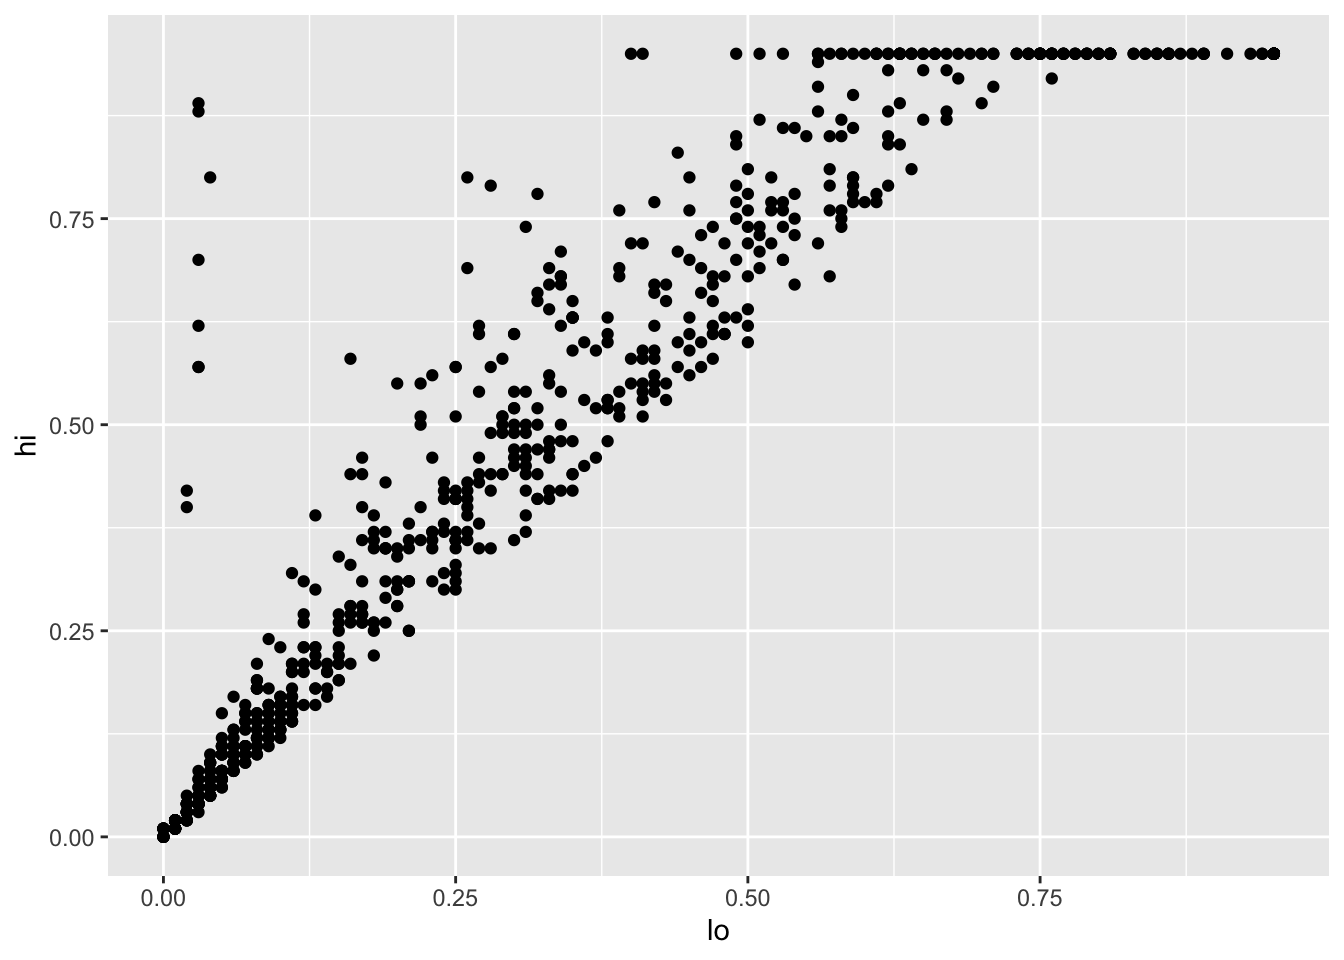
\includegraphics{tidyverse_files/figure-latex/basic-plot-1.pdf}

Looking more closely:

\begin{itemize}
\tightlist
\item
  The function \texttt{ggplot} creates an object to represent the chart with \texttt{infant\_hiv} as the underlying data.
\item
  \texttt{geom\_point} specifies the geometry we want (points).
\item
  Its \texttt{mapping} argument is assigned an \href{glossary.html\#aesthetic}{aesthetic}
  that specifies \texttt{lo} is to be used as the \texttt{x} coordinate and \texttt{hi} is to be used as the \texttt{y} coordinate.
\item
  The elements of the chart are combined with \texttt{+} rather than \texttt{\%\textgreater{}\%} for historical reasons.
\end{itemize}

Let's create a slightly more appealing plot by dropping NAs,
making the points semi-transparent,
and colorizing them according to the value of \texttt{estimate}:

\begin{Shaded}
\begin{Highlighting}[]
\NormalTok{infant_hiv }\OperatorTok
\StringTok{  }\KeywordTok{drop_na}\NormalTok{() }\OperatorTok
\StringTok{  }\KeywordTok{ggplot}\NormalTok{(}\DataTypeTok{mapping =} \KeywordTok{aes}\NormalTok{(}\DataTypeTok{x =}\NormalTok{ lo, }\DataTypeTok{y =}\NormalTok{ hi, }\DataTypeTok{color =}\NormalTok{ estimate)) }\OperatorTok{+}
\StringTok{  }\KeywordTok{geom_point}\NormalTok{(}\DataTypeTok{alpha =} \FloatTok{0.5}\NormalTok{) }\OperatorTok{+}
\StringTok{  }\KeywordTok{xlim}\NormalTok{(}\FloatTok{0.0}\NormalTok{, }\FloatTok{1.0}\NormalTok{) }\OperatorTok{+}\StringTok{ }\KeywordTok{ylim}\NormalTok{(}\FloatTok{0.0}\NormalTok{, }\FloatTok{1.0}\NormalTok{)}
\end{Highlighting}
\end{Shaded}

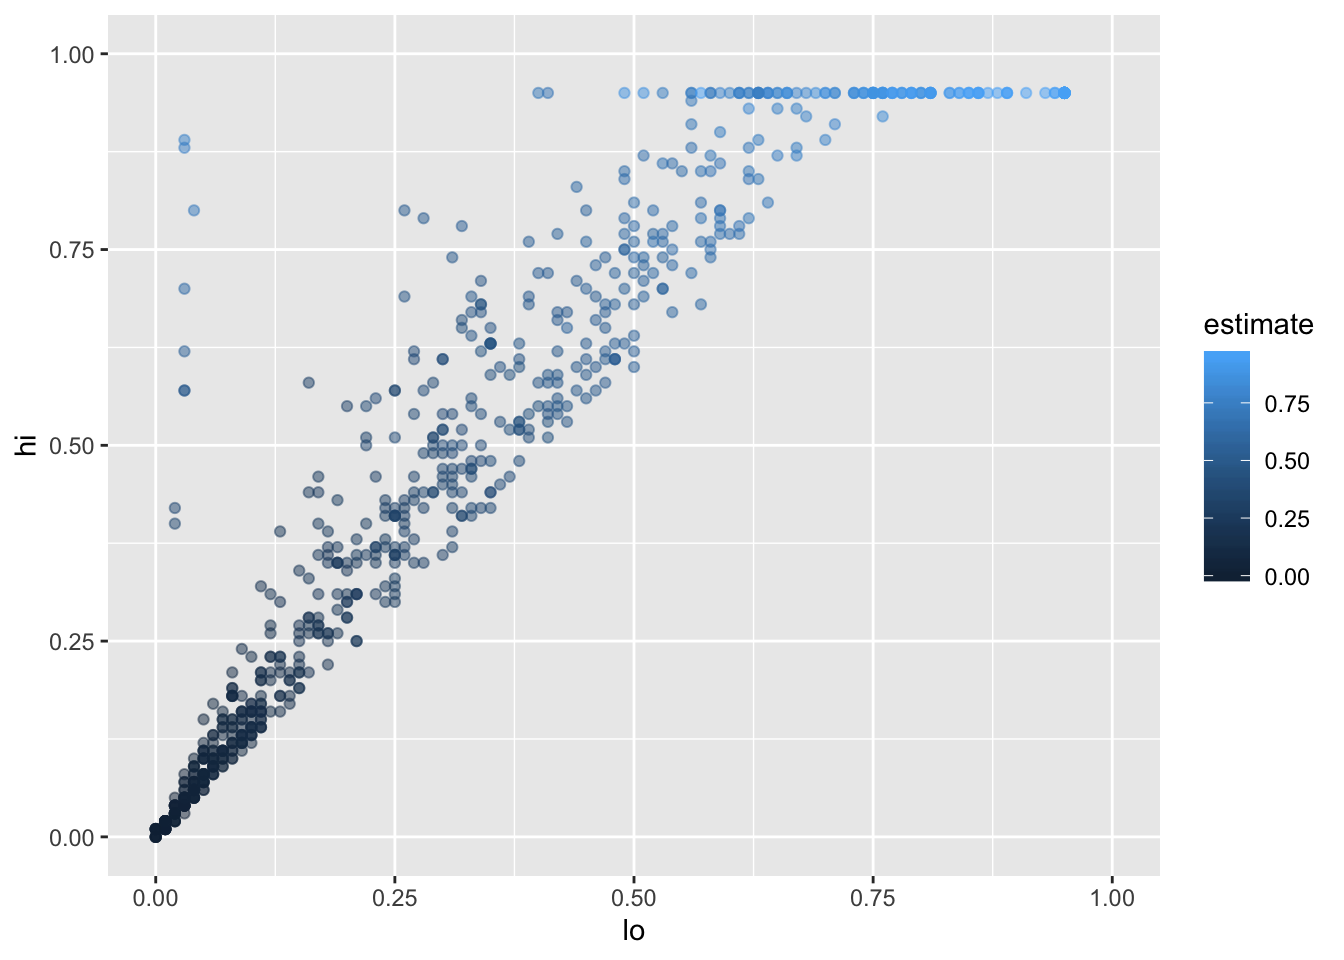
\includegraphics{tidyverse_files/figure-latex/plot-after-drop-1.pdf}

We set the transparency \texttt{alpha} outside the aesthetic because its value is constant for all points.
If we set it inside \texttt{aes(...)},
we would be telling ggplot2 to set the transparency according to the value of the data.
We specify the limits to the axes manually with \texttt{xlim} and \texttt{ylim} to ensure that ggplot2 includes the upper bounds:
without this,
all of the data would be shown,
but the upper label ``1.00'' would be omitted.

This plot immediately shows us that we have some outliers.
There are far more values with \texttt{hi} equal to 0.95 than it seems there ought to be,
and there are eight points running up the left margin that seem troubling as well.
Let's create a new tibble that doesn't have these:

\begin{Shaded}
\begin{Highlighting}[]
\NormalTok{infant_hiv }\OperatorTok
\StringTok{  }\KeywordTok{drop_na}\NormalTok{() }\OperatorTok
\StringTok{  }\KeywordTok{filter}\NormalTok{(hi }\OperatorTok{!=}\StringTok{ }\FloatTok{0.95}\NormalTok{) }\OperatorTok
\StringTok{  }\KeywordTok{filter}\NormalTok{(}\OperatorTok{!}\NormalTok{((lo }\OperatorTok{<}\StringTok{ }\FloatTok{0.10}\NormalTok{) }\OperatorTok{&}\StringTok{ }\NormalTok{(hi }\OperatorTok{>}\StringTok{ }\FloatTok{0.25}\NormalTok{))) }\OperatorTok
\StringTok{  }\KeywordTok{ggplot}\NormalTok{(}\DataTypeTok{mapping =} \KeywordTok{aes}\NormalTok{(}\DataTypeTok{x =}\NormalTok{ lo, }\DataTypeTok{y =}\NormalTok{ hi, }\DataTypeTok{color =}\NormalTok{ estimate)) }\OperatorTok{+}
\StringTok{  }\KeywordTok{geom_point}\NormalTok{(}\DataTypeTok{alpha =} \FloatTok{0.5}\NormalTok{) }\OperatorTok{+}
\StringTok{  }\KeywordTok{xlim}\NormalTok{(}\FloatTok{0.0}\NormalTok{, }\FloatTok{1.0}\NormalTok{) }\OperatorTok{+}\StringTok{ }\KeywordTok{ylim}\NormalTok{(}\FloatTok{0.0}\NormalTok{, }\FloatTok{1.0}\NormalTok{)}
\end{Highlighting}
\end{Shaded}

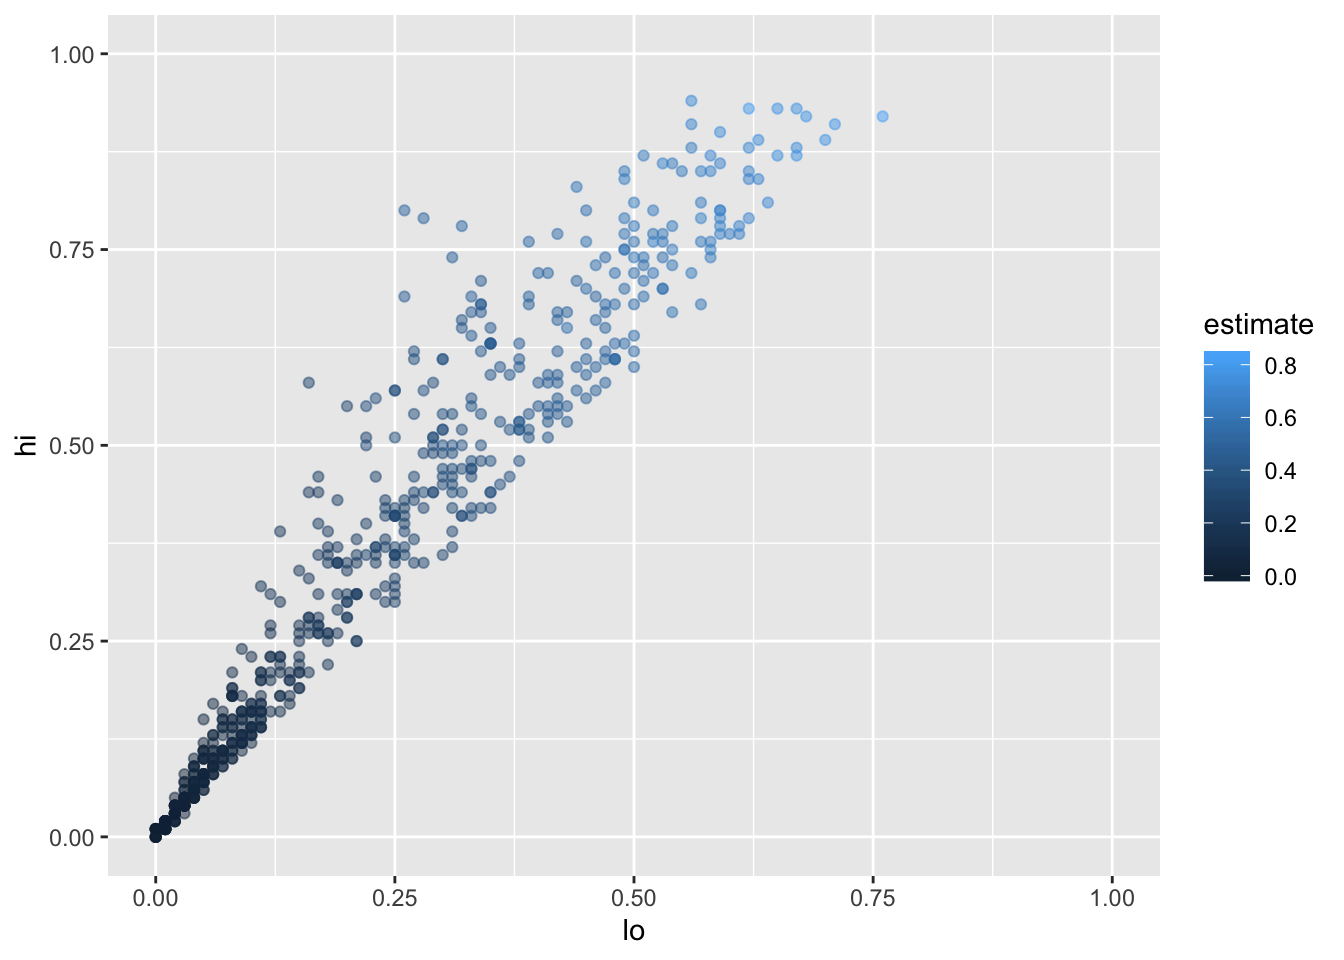
\includegraphics{tidyverse_files/figure-latex/plot-remove-outliers-1.pdf}

We can add the fitted curve by including another geometry called \texttt{geom\_smooth}:

\begin{Shaded}
\begin{Highlighting}[]
\NormalTok{infant_hiv }\OperatorTok
\StringTok{  }\KeywordTok{drop_na}\NormalTok{() }\OperatorTok
\StringTok{  }\KeywordTok{filter}\NormalTok{(hi }\OperatorTok{!=}\StringTok{ }\FloatTok{0.95}\NormalTok{) }\OperatorTok
\StringTok{  }\KeywordTok{filter}\NormalTok{(}\OperatorTok{!}\NormalTok{((lo }\OperatorTok{<}\StringTok{ }\FloatTok{0.10}\NormalTok{) }\OperatorTok{&}\StringTok{ }\NormalTok{(hi }\OperatorTok{>}\StringTok{ }\FloatTok{0.25}\NormalTok{))) }\OperatorTok
\StringTok{  }\KeywordTok{ggplot}\NormalTok{(}\DataTypeTok{mapping =} \KeywordTok{aes}\NormalTok{(}\DataTypeTok{x =}\NormalTok{ lo, }\DataTypeTok{y =}\NormalTok{ hi)) }\OperatorTok{+}
\StringTok{  }\KeywordTok{geom_point}\NormalTok{(}\DataTypeTok{mapping =} \KeywordTok{aes}\NormalTok{(}\DataTypeTok{color =}\NormalTok{ estimate), }\DataTypeTok{alpha =} \FloatTok{0.5}\NormalTok{) }\OperatorTok{+}
\StringTok{  }\KeywordTok{geom_smooth}\NormalTok{(}\DataTypeTok{method =}\NormalTok{ lm, }\DataTypeTok{color =} \StringTok{'red'}\NormalTok{) }\OperatorTok{+}
\StringTok{  }\KeywordTok{xlim}\NormalTok{(}\FloatTok{0.0}\NormalTok{, }\FloatTok{1.0}\NormalTok{) }\OperatorTok{+}\StringTok{ }\KeywordTok{ylim}\NormalTok{(}\FloatTok{0.0}\NormalTok{, }\FloatTok{1.0}\NormalTok{)}
\end{Highlighting}
\end{Shaded}

\begin{verbatim}
Warning: Removed 8 rows containing missing values (geom_smooth).
\end{verbatim}

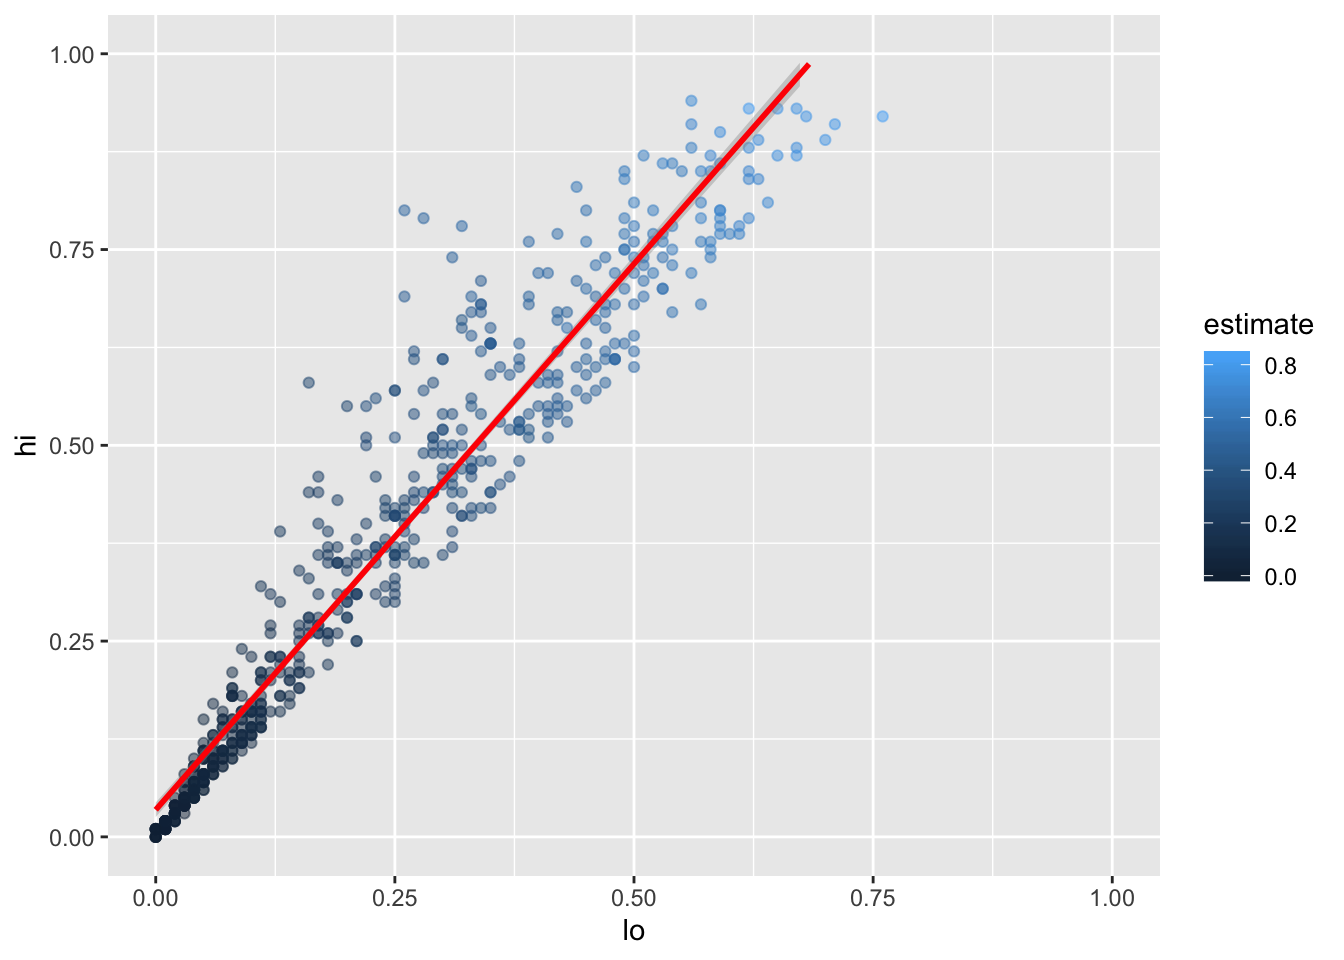
\includegraphics{tidyverse_files/figure-latex/plot-with-fit-1.pdf}

But wait:
why is this complaining about missing values?
Some online searches lead to the discovery that
\texttt{geom\_smooth} adds virtual points to the data for plotting purposes,
some of which lie outside the range of the actual data,
and that setting \texttt{xlim} and \texttt{ylim} then truncates these.
(Remember, R is differently sane\ldots{})
The safe way to control the range of the data is to add a call to \texttt{coord\_cartesian},
which effectively zooms in on a region of interest:

\begin{Shaded}
\begin{Highlighting}[]
\NormalTok{infant_hiv }\OperatorTok
\StringTok{  }\KeywordTok{drop_na}\NormalTok{() }\OperatorTok
\StringTok{  }\KeywordTok{filter}\NormalTok{(hi }\OperatorTok{!=}\StringTok{ }\FloatTok{0.95}\NormalTok{) }\OperatorTok
\StringTok{  }\KeywordTok{filter}\NormalTok{(}\OperatorTok{!}\NormalTok{((lo }\OperatorTok{<}\StringTok{ }\FloatTok{0.10}\NormalTok{) }\OperatorTok{&}\StringTok{ }\NormalTok{(hi }\OperatorTok{>}\StringTok{ }\FloatTok{0.25}\NormalTok{))) }\OperatorTok
\StringTok{  }\KeywordTok{ggplot}\NormalTok{(}\DataTypeTok{mapping =} \KeywordTok{aes}\NormalTok{(}\DataTypeTok{x =}\NormalTok{ lo, }\DataTypeTok{y =}\NormalTok{ hi)) }\OperatorTok{+}
\StringTok{  }\KeywordTok{geom_point}\NormalTok{(}\DataTypeTok{mapping =} \KeywordTok{aes}\NormalTok{(}\DataTypeTok{color =}\NormalTok{ estimate), }\DataTypeTok{alpha =} \FloatTok{0.5}\NormalTok{) }\OperatorTok{+}
\StringTok{  }\KeywordTok{geom_smooth}\NormalTok{(}\DataTypeTok{method =}\NormalTok{ lm, }\DataTypeTok{color =} \StringTok{'red'}\NormalTok{) }\OperatorTok{+}
\StringTok{  }\KeywordTok{coord_cartesian}\NormalTok{(}\DataTypeTok{xlim =} \KeywordTok{c}\NormalTok{(}\FloatTok{0.0}\NormalTok{, }\FloatTok{1.0}\NormalTok{), }\DataTypeTok{ylim =} \KeywordTok{c}\NormalTok{(}\FloatTok{0.0}\NormalTok{, }\FloatTok{1.0}\NormalTok{))}
\end{Highlighting}
\end{Shaded}

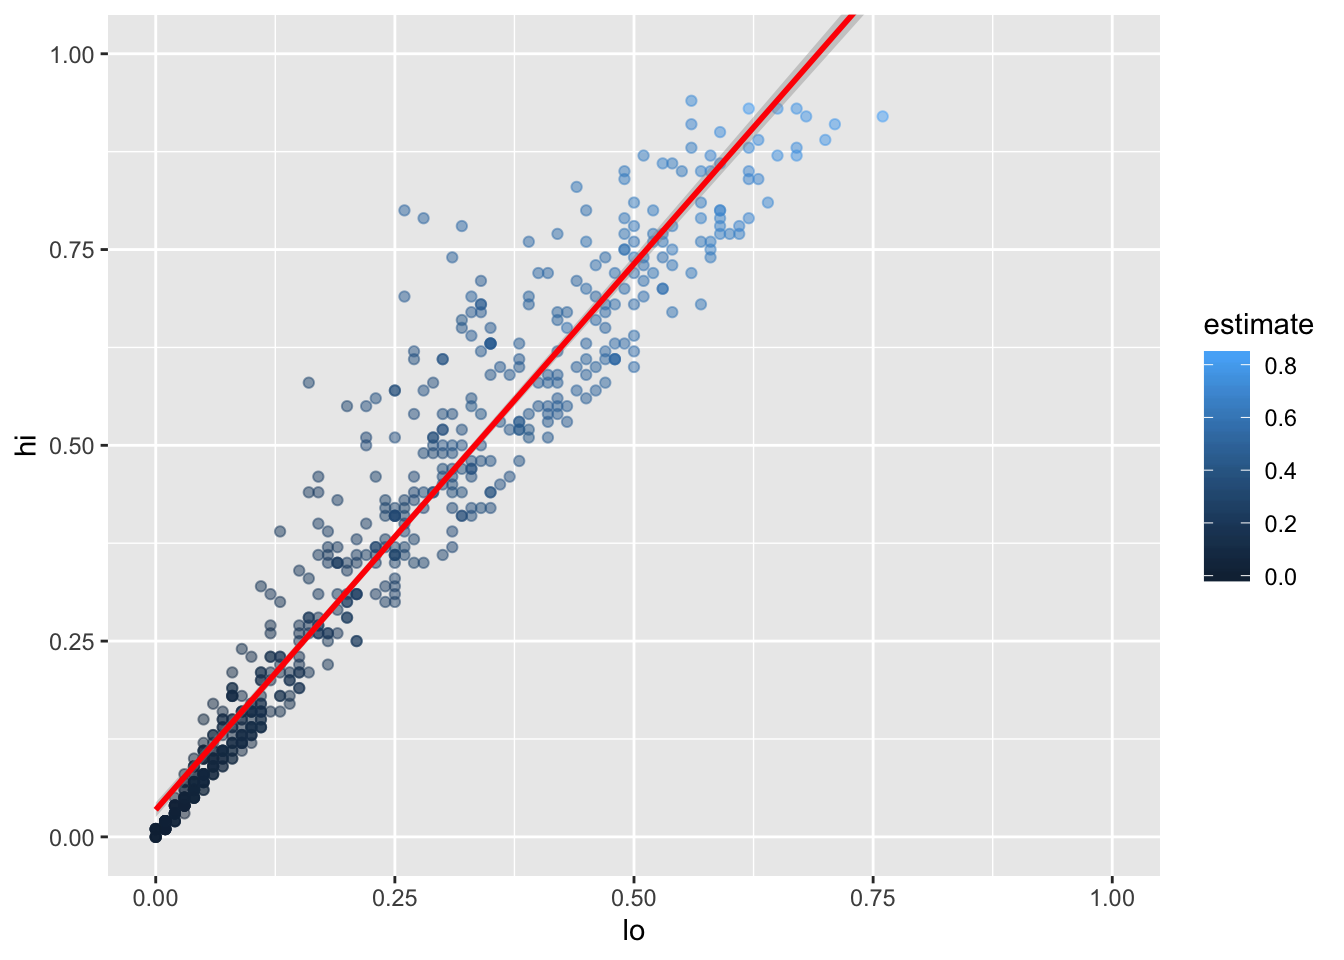
\includegraphics{tidyverse_files/figure-latex/plot-cartesian-1.pdf}

\hypertarget{do-i-need-more-practice-with-the-tidyverse}{%
\section{Do I need more practice with the tidyverse?}\label{do-i-need-more-practice-with-the-tidyverse}}

Absolutely:
open a fresh file and begin by loading the tidyverse
and the here package used to construct paths:

\begin{Shaded}
\begin{Highlighting}[]
\KeywordTok{library}\NormalTok{(tidyverse)}
\KeywordTok{library}\NormalTok{(here)}
\end{Highlighting}
\end{Shaded}

Next,
use \texttt{here::here} to construct a path to a file and \texttt{readr::read\_csv} to read that file:

\begin{Shaded}
\begin{Highlighting}[]
\NormalTok{path =}\StringTok{ }\NormalTok{here}\OperatorTok{::}\KeywordTok{here}\NormalTok{(}\StringTok{"data"}\NormalTok{, }\StringTok{"person.csv"}\NormalTok{)}
\NormalTok{person <-}\StringTok{ }\NormalTok{readr}\OperatorTok{::}\KeywordTok{read_csv}\NormalTok{(path)}
\end{Highlighting}
\end{Shaded}

\begin{verbatim}
Parsed with column specification:
cols(
  person_id = col_character(),
  personal_name = col_character(),
  family_name = col_character()
)
\end{verbatim}

We don't need to write out fully-qualified names---\texttt{here} and \texttt{read\_csv} will do---but
we will use them to make it easier to see what comes from where.

Next,
have a look at the tibble \texttt{person},
which contains some basic information about a group of foolhardy scientists
who ventured into the Antarctic in the 1920s and 1930s in search of things best left undisturbed:

\begin{Shaded}
\begin{Highlighting}[]
\NormalTok{person}
\end{Highlighting}
\end{Shaded}

\begin{verbatim}
# A tibble: 5 x 3
  person_id personal_name family_name
  <chr>     <chr>         <chr>      
1 dyer      William       Dyer       
2 pb        Frank         Pabodie    
3 lake      Anderson      Lake       
4 roe       Valentina     Roerich    
5 danforth  Frank         Danforth   
\end{verbatim}

How many rows and columns does this tibble contain?

\begin{Shaded}
\begin{Highlighting}[]
\KeywordTok{nrow}\NormalTok{(person)}
\end{Highlighting}
\end{Shaded}

\begin{verbatim}
[1] 5
\end{verbatim}

\begin{Shaded}
\begin{Highlighting}[]
\KeywordTok{ncol}\NormalTok{(person)}
\end{Highlighting}
\end{Shaded}

\begin{verbatim}
[1] 3
\end{verbatim}

(These names don't have a package prefix because they are built in.)
Let's show that information in a slightly nicer way
using \texttt{glue} to insert values into a string
and \texttt{print} to display the result:

\begin{Shaded}
\begin{Highlighting}[]
\KeywordTok{print}\NormalTok{(glue}\OperatorTok{::}\KeywordTok{glue}\NormalTok{(}\StringTok{"person has \{nrow(person)\} rows and \{ncol(person)\} columns"}\NormalTok{))}
\end{Highlighting}
\end{Shaded}

\begin{verbatim}
person has 5 rows and 3 columns
\end{verbatim}

If we want to display several values,
we can use the function \texttt{paste} to combine the elements of a vector.
\texttt{colnames} gives us the names of a tibble's columns,
and \texttt{paste}'s \texttt{collapse} argument tells the function
to use a single space to separate concatenated values:

\begin{Shaded}
\begin{Highlighting}[]
\KeywordTok{print}\NormalTok{(glue}\OperatorTok{::}\KeywordTok{glue}\NormalTok{(}\StringTok{"person columns are \{paste(colnames(person), collapse = ' ')\}"}\NormalTok{))}
\end{Highlighting}
\end{Shaded}

\begin{verbatim}
person columns are person_id personal_name family_name
\end{verbatim}

Time for some data manipulation.
Let's get everyone's family and personal names:

\begin{Shaded}
\begin{Highlighting}[]
\NormalTok{dplyr}\OperatorTok{::}\KeywordTok{select}\NormalTok{(person, family_name, personal_name)}
\end{Highlighting}
\end{Shaded}

\begin{verbatim}
# A tibble: 5 x 2
  family_name personal_name
  <chr>       <chr>        
1 Dyer        William      
2 Pabodie     Frank        
3 Lake        Anderson     
4 Roerich     Valentina    
5 Danforth    Frank        
\end{verbatim}

and then filter that list to keep only those that come in the first half of the alphabet:

\begin{Shaded}
\begin{Highlighting}[]
\NormalTok{dplyr}\OperatorTok{::}\KeywordTok{select}\NormalTok{(person, family_name, personal_name) }\OperatorTok
\StringTok{  }\NormalTok{dplyr}\OperatorTok{::}\KeywordTok{filter}\NormalTok{(family_name }\OperatorTok{<}\StringTok{ "N"}\NormalTok{)}
\end{Highlighting}
\end{Shaded}

\begin{verbatim}
# A tibble: 3 x 2
  family_name personal_name
  <chr>       <chr>        
1 Dyer        William      
2 Lake        Anderson     
3 Danforth    Frank        
\end{verbatim}

It would be more consistent to rewrite this as:

\begin{Shaded}
\begin{Highlighting}[]
\NormalTok{person }\OperatorTok
\StringTok{  }\NormalTok{dplyr}\OperatorTok{::}\KeywordTok{select}\NormalTok{(family_name, personal_name) }\OperatorTok
\StringTok{  }\NormalTok{dplyr}\OperatorTok{::}\KeywordTok{filter}\NormalTok{(family_name }\OperatorTok{<}\StringTok{ "N"}\NormalTok{)}
\end{Highlighting}
\end{Shaded}

\begin{verbatim}
# A tibble: 3 x 2
  family_name personal_name
  <chr>       <chr>        
1 Dyer        William      
2 Lake        Anderson     
3 Danforth    Frank        
\end{verbatim}

It's easy to add a column that records the lengths of family names:

\begin{Shaded}
\begin{Highlighting}[]
\NormalTok{person }\OperatorTok
\StringTok{  }\NormalTok{dplyr}\OperatorTok{::}\KeywordTok{mutate}\NormalTok{(}\DataTypeTok{name_length =}\NormalTok{ stringr}\OperatorTok{::}\KeywordTok{str_length}\NormalTok{(family_name))}
\end{Highlighting}
\end{Shaded}

\begin{verbatim}
# A tibble: 5 x 4
  person_id personal_name family_name name_length
  <chr>     <chr>         <chr>             <int>
1 dyer      William       Dyer                  4
2 pb        Frank         Pabodie               7
3 lake      Anderson      Lake                  4
4 roe       Valentina     Roerich               7
5 danforth  Frank         Danforth              8
\end{verbatim}

and then arrange in descending order:

\begin{Shaded}
\begin{Highlighting}[]
\NormalTok{person }\OperatorTok
\StringTok{  }\NormalTok{dplyr}\OperatorTok{::}\KeywordTok{mutate}\NormalTok{(}\DataTypeTok{name_length =}\NormalTok{ stringr}\OperatorTok{::}\KeywordTok{str_length}\NormalTok{(family_name)) }\OperatorTok
\StringTok{  }\NormalTok{dplyr}\OperatorTok{::}\KeywordTok{arrange}\NormalTok{(dplyr}\OperatorTok{::}\KeywordTok{desc}\NormalTok{(name_length))}
\end{Highlighting}
\end{Shaded}

\begin{verbatim}
# A tibble: 5 x 4
  person_id personal_name family_name name_length
  <chr>     <chr>         <chr>             <int>
1 danforth  Frank         Danforth              8
2 pb        Frank         Pabodie               7
3 roe       Valentina     Roerich               7
4 dyer      William       Dyer                  4
5 lake      Anderson      Lake                  4
\end{verbatim}

\hypertarget{key-points-1}{%
\section{Key Points}\label{key-points-1}}

\begin{itemize}
\tightlist
\item
  \texttt{install.packages(\textquotesingle{}name\textquotesingle{})} installs packages.
\item
  \texttt{library(name)} (without quoting the name) loads a package.
\item
  \texttt{library(tidyverse)} loads the entire collection of tidyverse libraries at once.
\item
  \texttt{read\_csv(filename)} reads CSV files that use the string `NA' to represent missing values.
\item
  \texttt{read\_csv} infers each column's data types based on the first thousand values it reads.
\item
  A tibble is the tidyverse's version of a data frame, which represents tabular data.
\item
  \texttt{head(tibble)} and \texttt{tail(tibble)} inspect the first and last few rows of a tibble.
\item
  \texttt{summary(tibble)} displays a summary of a tibble's structure and values.
\item
  \texttt{tibble\$column} selects a column from a tibble, returning a vector as a result.
\item
  \texttt{tibble{[}\textquotesingle{}column\textquotesingle{}{]}} selects a column from a tibble, returning a tibble as a result.
\item
  \texttt{tibble{[},c{]}} selects column \texttt{c} from a tibble, returning a tibble as a result.
\item
  \texttt{tibble{[}r,{]}} selects row \texttt{r} from a tibble, returning a tibble as a result.
\item
  Use ranges and logical vectors as indices to select multiple rows/columns or specific rows/columns from a tibble.
\item
  \texttt{tibble{[}{[}c{]}{]}} selects column \texttt{c} from a tibble, returning a vector as a result.
\item
  \texttt{min(...)}, \texttt{mean(...)}, \texttt{max(...)}, and \texttt{std(...)} calculates the minimum, mean, maximum, and standard deviation of data.
\item
  These aggregate functions include \texttt{NA}s in their calculations, and so will produce \texttt{NA} if the input data contains any.
\item
  Use \texttt{func(data,\ na.rm\ =\ TRUE)} to remove \texttt{NA}s from data before calculations are done (but make sure this is statistically justified).
\item
  \texttt{filter(tibble,\ condition)} selects rows from a tibble that pass a logical test on their values.
\item
  \texttt{arrange(tibble,\ column)} or \texttt{arrange(desc(column))} arrange rows according to values in a column (the latter in descending order).
\item
  \texttt{select(tibble,\ column,\ column,\ ...)} selects columns from a tibble.
\item
  \texttt{select(tibble,\ -column)} selects \emph{out} a column from a tibble.
\item
  \texttt{mutate(tibble,\ name\ =\ expression,\ name\ =\ expression,\ ...)} adds new columns to a tibble using values from existing columns.
\item
  \texttt{group\_by(tibble,\ column,\ column,\ ...)} groups rows that have the same values in the specified columns.
\item
  \texttt{summarize(tibble,\ name\ =\ expression,\ name\ =\ expression)} aggregates tibble values (by groups if the rows have been grouped).
\item
  \texttt{tibble\ \%\textgreater{}\%\ function(arguments)} performs the same operation as \texttt{function(tibble,\ arguments)}.
\item
  Use \texttt{\%\textgreater{}\%} to create pipelines in which the left side of each \texttt{\%\textgreater{}\%} becomes the first argument of the next stage.
\end{itemize}

\hypertarget{rmarkdown}{%
\chapter{Creating Reports}\label{rmarkdown}}

Every serious scholar dreams of recording their knowledge in a leather-bound tome
that will lie forgotten and dusty on the shelves of an out-of-the-way library
at a small college with a dubious reputation
until someone naïve enough to believe that they can control forces beyond mortal ken
stumbles upon it and unleashes ravenous horrors to prey upon the sanity of the innocent.
Sadly,
in these diminished times we must settle for dry expositions of trivia
typeset in two columns using a demure font and sequentially-numbered citations.

But there is yet hope.
One of R's greatest strengths is a package called \texttt{knitr}
that translates documents written in a format called R~Markdown into HTML, PDF, and e-books.
R~Markdown files are a kind of programmable document;
authors can interleave prose with chunks of R (or other languages)
and \texttt{knitr} will run that code as it processes the document
to create tables and diagrams.
To aid this,
the RStudio IDE includes tools to create new documents,
insert and run code chunks,
preview documents' structure and output,
and much more.

That's the good news.
The bad news is that Markdown isn't a standard:
it's more like a set of ad hoc implementations flying in loose formation.
While basic elements like headings and links are more or less the same in R~Markdown
as they are in (for example) \href{glossary.html\#gfm}{GitHub Flavored Markdown},
people who have used other dialects may trip over small differences.

This chapter starts by introducing Markdown and publishing workflow,
then shows how to embed code and customize reports.
We close by showing how to publish reports on GitHub and Netlify,
which both offer free hosting for small websites.

\hypertarget{learning-objectives-2}{%
\section{Learning Objectives}\label{learning-objectives-2}}

\begin{itemize}
\tightlist
\item
  Create a Markdown file that includes headings, links, and external images.
\item
  Compile that file to produce an HTML page.
\item
  Customize the page via its YAML header.
\item
  Add R code chunks to a page.
\item
  Format tabular output programmatically.
\item
  Share common startup code between pages.
\item
  Create and customize parameterized documents.
\item
  Publish pages on GitHub by putting generated HTML in the \texttt{docs} directory.
\item
  Publish pages by copying them to Netlify.
\end{itemize}

\hypertarget{how-can-i-create-and-preview-a-simple-page}{%
\section{How can I create and preview a simple page?}\label{how-can-i-create-and-preview-a-simple-page}}

To begin,
create a file called \texttt{first.Rmd} and add the following text to it:

\begin{Shaded}
\begin{Highlighting}[]
\FunctionTok{## Methods \{-\}}

\NormalTok{Something *really important*.}

\NormalTok{An }\OtherTok{[external link](https://tidynomicon.tech)}\NormalTok{.}

\OtherTok{[Another link][rstudio]}

\NormalTok{<!--}\CommentTok{ link table below -->}

\OtherTok{[rstudio]: https://rstudio.com}
\end{Highlighting}
\end{Shaded}

This shows several key features of Markdown:

\begin{itemize}
\tightlist
\item
  A level-1 heading (\texttt{h1} in HTML) is put on a line starting with \texttt{\#}.
  A level-2 heading (\texttt{h2}) uses two of these and so on.
\item
  Putting \texttt{\{-\}} immediately after the heading title suppresses numbering.
  Without this,
  our examples would all be included in this book's table of contents,
  which isn't what we want.
  (This is one of R~Markdown's extensions to Markdown.)
\item
  Paragraphs are separated by blank lines.
\item
  Text can be put in single asterisks for \emph{italics}
  or double asterisk for \textbf{bold}.
\item
  To create a link,
  put the visible text inside square brackets
  and the URL inside parentheses immediately after it.
  This is the reverse of HTML's order,
  which puts the URL inside the opening \texttt{a} tag
  \emph{before} the contained text that is displayed.
\item
  Links can also be written by putting text inside square brackets
  and an identifier immediately after it,
  also in square brackets.
  Those identifiers can then be associated with links in a table at the bottom of the page.
\item
  Comments are written as they are in HTML.
\end{itemize}

Here's what the HTML corresponding to our simple Markdown document looks like:

\begin{quote}
\hypertarget{methods}{%
\section*{Methods}\label{methods}}
\addcontentsline{toc}{section}{Methods}

Something \emph{really important}.

An \href{https://tidynomicon.tech}{external link}.

\href{https://rstudio.com}{Another link}
\end{quote}

To preview it,
go to the mini-toolbar at the top of your document in the RStudio IDE
and click ``knit'':
to call the appropriate function from \texttt{knitr}
(or a function from one of the libraries built on top of it for generating books or slides).

\begin{figure}
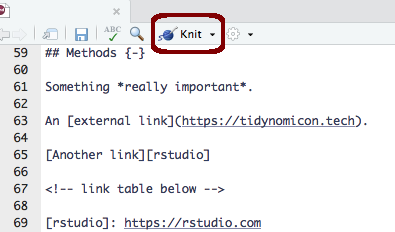
\includegraphics[width=5.49in]{figures/rmarkdown/knit-button} \caption{The 'knit' Button}\label{fig:knit-button}
\end{figure}

\hypertarget{how-can-i-run-code-and-include-its-output-in-a-page}{%
\section{How can I run code and include its output in a page?}\label{how-can-i-run-code-and-include-its-output-in-a-page}}

If this is all R~Markdown could do,
it would be nothing more than an idiosyncratic way to create HTML pages.
What makes it powerful is the ability to include code chunks
that are evaluated as the document is knit,
and whose output is included in the final page.
Put this in a file called \texttt{second.Rmd}:

\begin{Shaded}
\begin{Highlighting}[]
\NormalTok{Displaying the colors:}

\BaseNTok{```\{r\}}
\BaseNTok{colors <- c('red', 'green', 'blue')}
\BaseNTok{colors}
\BaseNTok{```}
\end{Highlighting}
\end{Shaded}

The triple back-quotes mark the start and end of a block of code;
putting \texttt{\{r\}} immediately after the back-quotes at the start
tells \texttt{knitr} to run the code
and include its output in the generated page,
which therefore looks like this:

Displaying the colors:

We can put any code we want inside code blocks.
We don't have to execute it all at once:
the \texttt{Code} pulldown in RStudio's main menu offers a variety of ways
to run regions of code.
The IDE also gives us a keyboard shortcut to insert a new code chunk,
so there really is no excuse for not making notes as we go along.

We can control execution and formatting by putting options inside the curly braces
at the start of the code block:

\begin{itemize}
\tightlist
\item
  \texttt{\{r\ label\}} gives the chunk a label that we can cross-reference.
  Labels must be unique within documents,
  just like the \texttt{id} attributes of HTML elements.
\item
  \texttt{\{r\ include=FALSE\}} tells \texttt{knitr} to run the code
  but \emph{not} to include either the code or its output in the finished document.
  While the option name is confusing---the code is actually included in processing---this
  is handy when we have setup code that loads libraries or does other things
  that our readers probably don't care about.
\item
  \texttt{\{r\ eval=FALSE\}} displays the code but doesn't run it,
  and is often used for tutorials like this one.
\item
  \texttt{\{r\ echo=FALSE\}} hides the code but includes the output.
  This is most often used for displaying static images
  as we will see below.
\end{itemize}

These options can be combined by separating them with commas.
In particular,
it's good style to give every chunk a unique label,
so a document might look like this:

\begin{Shaded}
\begin{Highlighting}[]
\FunctionTok{# My Thesis \{-\}}

\BaseNTok{```\{r setup, include=FALSE\}}
\BaseNTok{# Load tidyverse but don't display messages.}
\BaseNTok{library(tidyverse)}
\BaseNTok{```}

\BaseNTok{```\{r read-data, message=FALSE\}}
\BaseNTok{earthquakes <- read_csv('earthquakes.csv')}
\BaseNTok{```}

\NormalTok{A profound quotation to set the scene.}
\NormalTok{And then some analysis:}

\BaseNTok{```\{r calculate-depth-by-magnitude\}}
\BaseNTok{depth_by_magnitude <- earthquakes %>%}
\BaseNTok{  mutate(round_mag = round(Magnitude)) %>%}
\BaseNTok{  group_by(round_mag) %>%}
\BaseNTok{  summarize(depth = mean(Depth_Km))}
\BaseNTok{depth_by_magnitude}
\BaseNTok{```}

\NormalTok{Now let's visualize that:}

\BaseNTok{```\{r plot-depth-by-magnitude\}}
\BaseNTok{depth_by_magnitude %>%}
\BaseNTok{  ggplot() +}
\BaseNTok{  geom_point(mapping = aes(x = round_mag, y = depth))}
\BaseNTok{```}
\end{Highlighting}
\end{Shaded}

In order:

\begin{itemize}
\tightlist
\item
  The document title is a level-1 header with suppressed numbering.
\item
  The first code chunk is called \texttt{setup}
  and neither it nor its output are included in the output page.
\item
  The second chunk is called \texttt{read-data}.
  It is shown in the output,
  but its output is not.
\item
  There is then a (very) short paragraph.
\item
  The third code chunk calculates the mean depth by rounded magnitude.
  Both the code and its output are included;
  the output is just R's textual display of the \texttt{depth\_by\_magnitude} table.
\item
  After an even shorter paragraph,
  there is another named chunk whose output is a plot rather than text.
  \texttt{knitr} runs \texttt{ggplot2} to create the plot and includes it in the page.
\end{itemize}

When this page is knit,
the result is:

My Thesis

A profound quotation to set the scene. And then some analysis:

Now let's visualize that:

Note that if we want to include a static image (such as a screenshot) in a report,
we can use Markdown's own syntax:

\begin{Shaded}
\begin{Highlighting}[]
\AlertTok{![Summoning Ritual](figures/summoning-ritual.jpg)}
\end{Highlighting}
\end{Shaded}

or create an R code chunk with a call to \texttt{knitr::include\_graphics}:

\begin{Shaded}
\begin{Highlighting}[]
\BaseNTok{```\{r summoning-ritual, echo=FALSE, fig.cap="Summoning Ritual"\}}
\BaseNTok{knitr::include_graphics("figures/summoning-ritual.jpg")}
\BaseNTok{```}
\end{Highlighting}
\end{Shaded}

The options for the latter give the code chunk an ID,
prevent it from being echoed in the final document,
and most importantly,
give the figure a caption.
While it requires a bit of extra typing,
it produces more predictable results across different output formats.

\hypertarget{how-can-i-format-tables-in-a-page}{%
\section{How can I format tables in a page?}\label{how-can-i-format-tables-in-a-page}}

Tables are the undemonstrative yet reliable foundation on which data science is built.
While they are not as showy as their graphical counterparts,
they permit closer scrutiny,
and are accessible both to people with visual challenges
and to the machines whose inevitable triumph over us
shall usher in an agorithmic age free of superstition and mercy.

The simplest way to format tables is to use \texttt{knitr::kable}:

\begin{Shaded}
\begin{Highlighting}[]
\NormalTok{earthquakes }\OperatorTok
\StringTok{  }\KeywordTok{head}\NormalTok{(}\DecValTok{5}\NormalTok{) }\OperatorTok
\StringTok{  }\KeywordTok{kable}\NormalTok{()}
\end{Highlighting}
\end{Shaded}

\begin{tabular}{l|r|r|r|r}
\hline
Time & Latitude & Longitude & Depth\_Km & Magnitude\\
\hline
2016-08-24 03:36:32 & 42.6983 & 13.2335 & 8.1 & 6.0\\
\hline
2016-08-24 03:37:26 & 42.7123 & 13.2533 & 9.0 & 4.5\\
\hline
2016-08-24 03:40:46 & 42.7647 & 13.1723 & 9.7 & 3.8\\
\hline
2016-08-24 03:41:38 & 42.7803 & 13.1683 & 9.7 & 3.9\\
\hline
2016-08-24 03:42:07 & 42.7798 & 13.1575 & 9.7 & 3.6\\
\hline
\end{tabular}

Our output is more attractive if we install and load the \texttt{kableExtra} package
and use it to style the table.
We must call its functions \emph{after} we call \texttt{kable()},
just as we call the styling functions for plots after \texttt{ggplot()}.
Below,
we select four columns from our earthquake data and format them as a narrow table
with two decimal places for latitude and longitude,
one for magnitude and depth,
and some multi-column headers:

\begin{Shaded}
\begin{Highlighting}[]
\NormalTok{earthquakes }\OperatorTok
\StringTok{  }\KeywordTok{select}\NormalTok{(}\DataTypeTok{lat =}\NormalTok{ Latitude, }\DataTypeTok{long =}\NormalTok{ Longitude,}
         \DataTypeTok{mag =}\NormalTok{ Magnitude, }\DataTypeTok{depth =}\NormalTok{ Depth_Km) }\OperatorTok
\StringTok{  }\KeywordTok{head}\NormalTok{(}\DecValTok{5}\NormalTok{) }\OperatorTok
\StringTok{  }\KeywordTok{kable}\NormalTok{(}\DataTypeTok{digits =} \KeywordTok{c}\NormalTok{(}\DecValTok{2}\NormalTok{, }\DecValTok{2}\NormalTok{, }\DecValTok{1}\NormalTok{, }\DecValTok{1}\NormalTok{)) }\OperatorTok
\StringTok{  }\KeywordTok{kable_styling}\NormalTok{(}\DataTypeTok{full_width =} \OtherTok{FALSE}\NormalTok{) }\OperatorTok
\StringTok{  }\KeywordTok{add_header_above}\NormalTok{(}\KeywordTok{c}\NormalTok{(}\StringTok{'Location'}\NormalTok{ =}\StringTok{ }\DecValTok{2}\NormalTok{, }\StringTok{'Details'}\NormalTok{ =}\StringTok{ }\DecValTok{2}\NormalTok{))}
\end{Highlighting}
\end{Shaded}

\begin{table}[H]
\centering
\begin{tabular}{r|r|r|r}
\hline
\multicolumn{2}{c|}{Location} & \multicolumn{2}{c}{Details} \\
\cline{1-2} \cline{3-4}
lat & long & mag & depth\\
\hline
42.70 & 13.23 & 6.0 & 8.1\\
\hline
42.71 & 13.25 & 4.5 & 9.0\\
\hline
42.76 & 13.17 & 3.8 & 9.7\\
\hline
42.78 & 13.17 & 3.9 & 9.7\\
\hline
42.78 & 13.16 & 3.6 & 9.7\\
\hline
\end{tabular}
\end{table}

\hypertarget{how-can-i-share-code-between-pages}{%
\section{How can I share code between pages?}\label{how-can-i-share-code-between-pages}}

If you are working on several related reports,
you may want to share some code between them.
The best way to do this with R~Markdown is to put that code in a separate \texttt{.R} file
and then load that at the start of each document using the \texttt{source} function.
For example,
all of the chapters in this book begin with:

\begin{Shaded}
\begin{Highlighting}[]
\BaseNTok{```\{r setup, include=FALSE\}}
\BaseNTok{source('common.R')}
\BaseNTok{```}
\end{Highlighting}
\end{Shaded}

The chunk is named \texttt{setup}, and neither it nor its output are displayed.
All the chunk does is load and run \texttt{common.R},
which contains the following lines:

\begin{Shaded}
\begin{Highlighting}[]
\KeywordTok{library}\NormalTok{(tidyverse)}
\KeywordTok{library}\NormalTok{(reticulate)}
\KeywordTok{library}\NormalTok{(rlang)}
\KeywordTok{library}\NormalTok{(knitr)}

\NormalTok{knitr}\OperatorTok{::}\NormalTok{opts_knit}\OperatorTok{$}\KeywordTok{set}\NormalTok{(}\DataTypeTok{width =} \DecValTok{69}\NormalTok{)}
\end{Highlighting}
\end{Shaded}

The first few load libraries that various chapters depend on;
the last one tells \texttt{knitr} to set the line width option to 69 characters.

\hypertarget{how-can-i-parameterize-documents}{%
\section{How can I parameterize documents?}\label{how-can-i-parameterize-documents}}

\texttt{knitr} has many other options besides line width,
and the tools built on top of it,
like \href{https://bookdown.org/yihui/blogdown/}{Blogdown} and \href{https://bookdown.org/}{Bookdown},
have many (many) more.
Rather than calling a function to set them,
you can and should add a header to each document.
If we use \texttt{File...New\ File...RMarkdown} to create a new R~Markdown file,
its header looks like this:

\begin{Shaded}
\begin{Highlighting}[]
\NormalTok{---}
\NormalTok{title: "fourth"}
\NormalTok{author: "Greg Wilson"}
\NormalTok{date: "18/09/2019"}
\NormalTok{output: html_document}
\NormalTok{---}
\end{Highlighting}
\end{Shaded}

\begin{enumerate}
\def\labelenumi{\arabic{enumi}.}
\tightlist
\item
  The header starts with exactly three dashes on a line of their own and ends the same way.
  A common mistake is to forget the closing dashes;
  another is to use too many or too few,
  or to include whitespace in the line.
\item
  The content of the header is formatted using \href{https://yaml.org/}{YAML},
  which stands for ``Yet Another Markup Language''.
  In its simplest form it contains key-value pairs:
  the keys are words,
  the values can be numbers, quoted strings, or a variety of other things,
  and the two are separated by a comma.
\end{enumerate}

This header tells \texttt{knitr} what the document's title is,
who its author is,
when it was created
(which really ought to be written as an ISO-formatted date, but worse sins await us),
and what output format we want by default.
When we knit the document,
\texttt{knitr} reads the header but does \emph{not} include it in the output.
Instead,
its values control \texttt{knitr}'s operation (e.g., select HTML as the output format)
or are inserted into the document itself (e.g., the title).

Let's edit the YAML header so that it looks like this:

\begin{Shaded}
\begin{Highlighting}[]
\NormalTok{---}
\NormalTok{title: "fourth"}
\NormalTok{author: "Greg Wilson"}
\NormalTok{date: "2019-09-18"}
\NormalTok{output:}
\NormalTok{  html_document:}
\BaseNTok{    theme: united}
\BaseNTok{    toc: true}
\NormalTok{---}
\end{Highlighting}
\end{Shaded}

\begin{enumerate}
\def\labelenumi{\arabic{enumi}.}
\tightlist
\item
  The date is now in an unambiguous, sortable format.
  This doesn't impact our document,
  but makes us feel better.
\item
  We have added two sub-keys under \texttt{html\_document}
  (which we have made a sub-key of \texttt{output} so that we can nest things beneath it).
  The first tells \texttt{knitr} to use the \texttt{united} theme,
  which gives us a different set of fonts and margins.
  The second tells it to create a table of contents at the start of the document
  with links to all of the section headers.
\end{enumerate}

YAML can \href{http://third-bit.com/2015/06/11/why-we-cant-have-nice-things.html}{be quite complicated to understand}.
Luckily,
a package called \texttt{ymlthis} is being developed to create and check files' headers.
\href{https://ymlthis.r-lib.org/}{Its documentation} and capabilities are both steadily growing,
it's a great way to experiment with new or obscure options.

But YAML can do more than control the way \texttt{knitr} processes the document:
we can also use it to create \href{glossary.html\#parameterized-report}{parameterized reports}.

\begin{Shaded}
\begin{Highlighting}[]
\NormalTok{---}
\NormalTok{title: "Fifth Report"}
\NormalTok{params:}
\NormalTok{  country: Canada}
\NormalTok{---}

\NormalTok{This report looks at defenstration rates in }\BaseNTok{`r params$country`}\NormalTok{.}

\BaseNTok{```\{r load-data\}}
\BaseNTok{data <- read_csv(here::here('data', glue(params$country, '.csv')))}
\BaseNTok{```}
\end{Highlighting}
\end{Shaded}

This document's YAML header contains the key \texttt{params},
under which is a sub-key for each parameter we want to create.
When the document is knit,
these parameters are put in a \href{glossary.html\#named-list}{named list} called \texttt{params}
and can be referred to like any other variable.
If we want to display it inline,
we use a back-ticked code fragment that starts with the letter `r';
if we want to use it in a fenced code block,
it's no different from any other variable.

Parameters don't have to be single values:
they can, for example, be lists of mysterious ailments whose inexorable spread you are vainly trying to halt.
Parameters can also be provided on the command line:

\begin{verbatim}
Rscript -e "rmarkdown::render('fifth.Rmd', params=list(country='Lesotho'))"
\end{verbatim}

will create a page called \texttt{fifth.html} that reports defenestration rates in Lesotho.

\hypertarget{how-can-i-publish-pages-on-github}{%
\section{How can I publish pages on GitHub?}\label{how-can-i-publish-pages-on-github}}

Many programmers use \href{https://pages.github.com/}{GitHub Pages} to publish websites
for project documentation, personal blogs,
and desperate entreaties to other-worldly forces
(Iä! Iä! Git rebase fhtagn!).
In its original incarnation,
GitHub Pages worked used as follows:

\begin{enumerate}
\def\labelenumi{\arabic{enumi}.}
\tightlist
\item
  Authors created Markdown and HTML files with content they want to publish.
  They also created a configuration file called \texttt{\_config.yml}
  with settings for their site (such as its title).
\item
  All of this was put on a Git branch called \texttt{gh-pages}.
  Whenever that branch was updated on GitHub,
  a \href{glossary.html\#static-site-generator}{static site generator} called \href{https://jekyllrb.com/}{Jekyll}
  would find and transform those files
  using templates and inclusions taken from the \texttt{\_layouts} and \texttt{\_includes} directories respectively.
\end{enumerate}

Keeping the \texttt{gh-pages} branch synchronized with other work proved to be a minor headache,
so GitHub now offers two other options
(which can be configured from a project's settings in the GitHub browser interface):

\begin{enumerate}
\def\labelenumi{\arabic{enumi}.}
\tightlist
\item
  Publish directly from the root directory of the project's \texttt{master} branch.
\item
  Publish from the \texttt{docs} folder in the \texttt{master} branch.
\end{enumerate}

One other piece of background is how Jekyll determines what to publish:

\begin{itemize}
\tightlist
\item
  It ignores files and directories whose names start with an underscore,
  or that it is specifically told to exclude in \texttt{\_config.yml}.
\item
  If an HTML or Markdown file starts with a YAML header,
  Jekyll translates it.
\item
  If the file does not include such a header,
  Jekyll simply copies it as-is.
\end{itemize}

All of this gives us a simple way to publish an R~Markdown website:

\begin{enumerate}
\def\labelenumi{\arabic{enumi}.}
\tightlist
\item
  Make sure the project is configured to publish from the root directory of the \texttt{master} branch.
\item
  Compile our R~Markdown files locally to create HTML in the root directory of our local copy.
\item
  Commit that HTML to the \texttt{master} branch.
\item
  Push.
\end{enumerate}

This works because the HTML files generated by \texttt{knitr} don't contain YAML headers,
so they are copied as-is.
If we want to style those pages with our own CSS or add some JavaScript,
we can tell \texttt{knitr} to include files of our choice during translation:

\begin{Shaded}
\begin{Highlighting}[]
\NormalTok{---}
\NormalTok{title: "Defenestration By Country"}
\NormalTok{output:}
\NormalTok{  html_document:}
\BaseNTok{    includes:}
\BaseNTok{      in_header: extra-header.html}
\BaseNTok{      after_body: extra-footer.html}
\NormalTok{---}
\NormalTok{...content...}
\end{Highlighting}
\end{Shaded}

Behind the scenes,
\texttt{knitr} translates our R~Markdown into plain Markdown,
which is then turned into HTML by yet another tool called \href{https://pandoc.org/}{Pandoc}.
If we are brave,
we can create an entirely new Pandoc HTML template and format our files with that:

\begin{Shaded}
\begin{Highlighting}[]
\NormalTok{---}
\NormalTok{title: "Defenestration by Season"}
\NormalTok{output:}
\NormalTok{  html_document:}
\BaseNTok{    template: seasonal-report.html}
\NormalTok{---}
\NormalTok{...content...}
\end{Highlighting}
\end{Shaded}

This works,
but having the generated HTML in our root directory is messy.
Given that we can configure GitHub Pages to publish from the \texttt{docs} folder,
why don't we put our HTML there?
After all,
\texttt{knitr::knit} has an \texttt{output} parameter with which we can specify a location for the output file.

The answer is that \texttt{knitr} becomes rather vexed when the output directory is not the same as
the current working directory.
Programmers being programmers,
there are several ways around this:

\begin{enumerate}
\def\labelenumi{\arabic{enumi}.}
\tightlist
\item
  Put up with it.
\item
  Write a small function that changes the current wording directory to \texttt{docs},
  knits \texttt{../report.Rmd},
  then changes the working directory back to the project root.
\item
  Use something like \href{https://www.gnu.org/software/make/}{Make} to build everything on the command line
  and then move all the generated files into \texttt{docs}.
\end{enumerate}

None of this is made any less frustrating by the fact that other tools in the \texttt{knitr} family,
such as Bookdown,
\emph{do} allow users to specify the output directory through a configuration parameter.

\hypertarget{key-points-2}{%
\section{Key Points}\label{key-points-2}}

\begin{itemize}
\tightlist
\item
  FIXME: key points for R~Markdown
\end{itemize}

\hypertarget{package}{%
\chapter{Creating Packages}\label{package}}

Data is not born tidy.
We must cleanse it to make it serve our needs.
The previous chapter gave us the tools;
here,
we will see how to apply them
and how to make our work usable by others.

\hypertarget{learning-objectives-3}{%
\section{Learning Objectives}\label{learning-objectives-3}}

\begin{itemize}
\tightlist
\item
  Describe and use the \texttt{read\_csv} function.
\item
  Describe and use the \texttt{str\_replace} function.
\item
  Describe and use the \texttt{is.numeric} and \texttt{as.numeric} functions.
\item
  Describe and use the \texttt{map} function and its kin.
\item
  Describe and use pre-allocation to capture the results of loops.
\item
  Describe the three things an R package can contain.
\item
  Explain how R code in a package is distributed and one implication of this.
\item
  Explain the purpose of the \texttt{DESCRIPTION}, \texttt{NAMESPACE} and \texttt{.Rbuildignore} files in an R project.
\item
  Explain what should be put in the \texttt{R}, \texttt{data}, \texttt{man}, and \texttt{tests} directories of an R project.
\item
  Describe and use specially-formatted comments with roxygen2 to document a package.
\item
  Use \texttt{@export} and \texttt{@import} directives correctly in roxygen2 documentation.
\item
  Add a dataset to an R package.
\item
  Use functions from external libraries inside a package in a hygienic way.
\item
  Rewrite references to bare column names to satisfy R's packaging checks.
\item
  Correctly document the package as a whole and the datasets it contains.
\end{itemize}

\hypertarget{what-is-our-starting-point}{%
\section{What is our starting point?}\label{what-is-our-starting-point}}

Here is a sample of data from the original data set \texttt{data/infant\_hiv.csv},
where \texttt{...} shows values elided to make the segment readable:

\begin{verbatim}
"Early Infant Diagnosis: Percentage of infants born to women living with HIV...",,,,,,,,,,,,,,,,,,,,,,,,,,,,,
,,2009,,,2010,,,2011,,,2012,,,2013,,,2014,,,2015,,,2016,,,2017,,,
ISO3,Countries,Estimate,hi,lo,Estimate,hi,lo,Estimate,hi,lo,Estimate,hi,lo,...
AFG,Afghanistan,-,-,-,-,-,-,-,-,-,-,-,-,-,-,-,-,-,-,-,-,-,-,-,-,-,-,-,
ALB,Albania,-,-,-,-,-,-,-,-,-,-,-,-,-,-,-,-,-,-,-,-,-,-,-,-,-,-,-,
DZA,Algeria,-,-,-,-,-,-,38%,42%,35%,23%,25%,21%,55%,60%,50%,27%,30%,25%,23%,25%,21%,33%,37%,31%,61%,68%,57%,
AGO,Angola,-,-,-,3%,4%,2%,5%,7%,4%,6%,8%,5%,15%,20%,12%,10%,14%,8%,6%,8%,5%,1%,2%,1%,1%,2%,1%,
... many more rows ...
YEM,Yemen,-,-,-,-,-,-,-,-,-,-,-,-,-,-,-,-,-,-,-,-,-,-,-,-,-,-,-,
ZMB,Zambia,59%,70%,53%,27%,32%,24%,70%,84%,63%,74%,88%,67%,64%,76%,57%,91%,>95%,81%,43%,52%,39%,43%,51%,39%,46%,54%,41%,
ZWE,Zimbabwe,-,-,-,12%,15%,10%,23%,28%,20%,38%,47%,33%,57%,70%,49%,54%,67%,47%,59%,73%,51%,71%,88%,62%,65%,81%,57%,
,,,,,,,,,,,,,,,,,,,,,,,,,,,,,
,,2009,,,2010,,,2011,,,2012,,,2013,,,2014,,,2015,,,2016,,,2017,,,
,,Estimate,hi,lo,Estimate,hi,lo,Estimate,hi,lo,Estimate,hi,lo,...
Region,East Asia and the Pacific,25%,30%,22%,35%,42%,29%,30%,37%,26%,32%,38%,27%,28%,34%,24%,26%,31%,22%,31%,37%,27%,30%,35%,25%,28%,33%,24%,
,Eastern and Southern Africa,23%,29%,20%,44%,57%,37%,48%,62%,40%,54%,69%,46%,51%,65%,43%,62%,80%,53%,62%,79%,52%,54%,68%,45%,62%,80%,53%,
,Eastern Europe and Central Asia,-,-,-,-,-,-,-,-,-,-,-,-,-,-,-,-,-,-,-,-,-,-,-,-,-,-,-,
... several more rows ...
,Sub-Saharan Africa,16%,22%,13%,34%,46%,28%,37%,50%,30%,43%,57%,35%,41%,54%,33%,50%,66%,41%,50%,66%,41%,45%,60%,37%,52%,69%,42%,
,Global,17%,23%,13%,33%,45%,27%,36%,49%,29%,41%,55%,34%,40%,53%,32%,48%,64%,39%,49%,64%,40%,44%,59%,36%,51%,67%,41%,
,,,,,,,,,,,,,,,,,,,,,,,,,,,,,
Indicator definition: Percentage of infants born to women living with HIV... ,,,,,,,,,,,,,,,,,,,,,,,,,,,,,
Note: Data are not available if country did not submit data...,,,,,,,,,,,,,,,,,,,,,,,,,,,,,
Data source: Global AIDS Monitoring 2018 and UNAIDS 2018 estimates,,,,,,,,,,,,,,,,,,,,,,,,,,,,,
"For more information on this indicator, please visit the guidance:...",,,,,,,,,,,,,,,,,,,,,,,,,,,,,
"For more information on the data, visit data.unicef.org",,,,,,,,,,,,,,,,,,,,,,,,,,,,,
\end{verbatim}

This is a mess---no, more than that, it is an affront to decency.
There are comments mixed with data,
values' actual indices have to be synthesized by combining column headings from two rows
(two thirds of which have to be carried forward from previous columns),
and so on.
We want to create the tidy data found in \texttt{results/infant\_hiv.csv}:

\begin{verbatim}
country,year,estimate,hi,lo
AFG,2009,NA,NA,NA
AFG,2010,NA,NA,NA
AFG,2011,NA,NA,NA
AFG,2012,NA,NA,NA
...
ZWE,2016,0.71,0.88,0.62
ZWE,2017,0.65,0.81,0.57
\end{verbatim}

\hypertarget{how-do-i-convert-values-to-numbers}{%
\section{How do I convert values to numbers?}\label{how-do-i-convert-values-to-numbers}}

We begin by reading the data into a tibble:

\begin{Shaded}
\begin{Highlighting}[]
\NormalTok{raw <-}\StringTok{ }\KeywordTok{read_csv}\NormalTok{(}\StringTok{"data/infant_hiv.csv"}\NormalTok{)}
\end{Highlighting}
\end{Shaded}

\begin{verbatim}
Warning: Missing column names filled in: 'X2' [2], 'X3' [3], 'X4' [4],
'X5' [5], 'X6' [6], 'X7' [7], 'X8' [8], 'X9' [9], 'X10' [10], 'X11' [11],
'X12' [12], 'X13' [13], 'X14' [14], 'X15' [15], 'X16' [16], 'X17' [17],
'X18' [18], 'X19' [19], 'X20' [20], 'X21' [21], 'X22' [22], 'X23' [23],
'X24' [24], 'X25' [25], 'X26' [26], 'X27' [27], 'X28' [28], 'X29' [29],
'X30' [30]
\end{verbatim}

\begin{verbatim}
Parsed with column specification:
cols(
  .default = col_character(),
  X30 = col_logical()
)
\end{verbatim}

\begin{verbatim}
See spec(...) for full column specifications.
\end{verbatim}

\begin{Shaded}
\begin{Highlighting}[]
\KeywordTok{head}\NormalTok{(raw)}
\end{Highlighting}
\end{Shaded}

\begin{verbatim}
# A tibble: 6 x 30
  `Early Infant D~ X2    X3    X4    X5    X6    X7    X8    X9    X10  
  <chr>            <chr> <chr> <chr> <chr> <chr> <chr> <chr> <chr> <chr>
1 <NA>             <NA>  2009  <NA>  <NA>  2010  <NA>  <NA>  2011  <NA> 
2 ISO3             Coun~ Esti~ hi    lo    Esti~ hi    lo    Esti~ hi   
3 AFG              Afgh~ -     -     -     -     -     -     -     -    
4 ALB              Alba~ -     -     -     -     -     -     -     -    
5 DZA              Alge~ -     -     -     -     -     -     38%   42%  
6 AGO              Ango~ -     -     -     3%    4%    2%    5%    7%   
# ... with 20 more variables: X11 <chr>, X12 <chr>, X13 <chr>, X14 <chr>,
#   X15 <chr>, X16 <chr>, X17 <chr>, X18 <chr>, X19 <chr>, X20 <chr>,
#   X21 <chr>, X22 <chr>, X23 <chr>, X24 <chr>, X25 <chr>, X26 <chr>,
#   X27 <chr>, X28 <chr>, X29 <chr>, X30 <lgl>
\end{verbatim}

All right:
R isn't able to infer column names,
so it uses the entire first comment string as a very long column name
and then makes up names for the other columns.
Looking at the file,
the second row has years (spaced at three-column intervals)
and the column after that has the \href{glossary.html\#iso3-country-code}{ISO3 country code},
the country's name,
and then ``Estimate'', ``hi'', and ``lo'' repeated for every year.
We are going to have to combine what's in the second and third rows,
so we're going to have to do some work no matter which we skip or keep.
Since we want the ISO3 code and the country name,
let's skip the first two rows.

\begin{Shaded}
\begin{Highlighting}[]
\NormalTok{raw <-}\StringTok{ }\KeywordTok{read_csv}\NormalTok{(}\StringTok{"data/infant_hiv.csv"}\NormalTok{, }\DataTypeTok{skip =} \DecValTok{2}\NormalTok{)}
\end{Highlighting}
\end{Shaded}

\begin{verbatim}
Warning: Missing column names filled in: 'X30' [30]
\end{verbatim}

\begin{verbatim}
Warning: Duplicated column names deduplicated: 'Estimate' =>
'Estimate_1' [6], 'hi' => 'hi_1' [7], 'lo' => 'lo_1' [8], 'Estimate' =>
'Estimate_2' [9], 'hi' => 'hi_2' [10], 'lo' => 'lo_2' [11], 'Estimate' =>
'Estimate_3' [12], 'hi' => 'hi_3' [13], 'lo' => 'lo_3' [14], 'Estimate' =>
'Estimate_4' [15], 'hi' => 'hi_4' [16], 'lo' => 'lo_4' [17], 'Estimate' =>
'Estimate_5' [18], 'hi' => 'hi_5' [19], 'lo' => 'lo_5' [20], 'Estimate' =>
'Estimate_6' [21], 'hi' => 'hi_6' [22], 'lo' => 'lo_6' [23], 'Estimate' =>
'Estimate_7' [24], 'hi' => 'hi_7' [25], 'lo' => 'lo_7' [26], 'Estimate' =>
'Estimate_8' [27], 'hi' => 'hi_8' [28], 'lo' => 'lo_8' [29]
\end{verbatim}

\begin{verbatim}
Parsed with column specification:
cols(
  .default = col_character(),
  X30 = col_logical()
)
\end{verbatim}

\begin{verbatim}
See spec(...) for full column specifications.
\end{verbatim}

\begin{Shaded}
\begin{Highlighting}[]
\KeywordTok{head}\NormalTok{(raw)}
\end{Highlighting}
\end{Shaded}

\begin{verbatim}
# A tibble: 6 x 30
  ISO3  Countries Estimate hi    lo    Estimate_1 hi_1  lo_1  Estimate_2
  <chr> <chr>     <chr>    <chr> <chr> <chr>      <chr> <chr> <chr>     
1 AFG   Afghanis~ -        -     -     -          -     -     -         
2 ALB   Albania   -        -     -     -          -     -     -         
3 DZA   Algeria   -        -     -     -          -     -     38%       
4 AGO   Angola    -        -     -     3%         4%    2%    5%        
5 AIA   Anguilla  -        -     -     -          -     -     -         
6 ATG   Antigua ~ -        -     -     -          -     -     -         
# ... with 21 more variables: hi_2 <chr>, lo_2 <chr>, Estimate_3 <chr>,
#   hi_3 <chr>, lo_3 <chr>, Estimate_4 <chr>, hi_4 <chr>, lo_4 <chr>,
#   Estimate_5 <chr>, hi_5 <chr>, lo_5 <chr>, Estimate_6 <chr>,
#   hi_6 <chr>, lo_6 <chr>, Estimate_7 <chr>, hi_7 <chr>, lo_7 <chr>,
#   Estimate_8 <chr>, hi_8 <chr>, lo_8 <chr>, X30 <lgl>
\end{verbatim}

That's a bit of an improvement,
but why are all the columns \texttt{character} instead of numbers?
This happens because:

\begin{enumerate}
\def\labelenumi{\arabic{enumi}.}
\tightlist
\item
  our CSV file uses \texttt{-} (a single dash) to show missing data, and
\item
  all of our numbers end with \texttt{\%}, which means those values actually \emph{are} character strings.
\end{enumerate}

We will tackle the first problem by setting \texttt{na\ =\ c("-")} in our \texttt{read\_csv} call
(since we should never do ourselves what a library function will do for us):

\begin{Shaded}
\begin{Highlighting}[]
\NormalTok{raw <-}\StringTok{ }\KeywordTok{read_csv}\NormalTok{(}\StringTok{"data/infant_hiv.csv"}\NormalTok{, }\DataTypeTok{skip =} \DecValTok{2}\NormalTok{, }\DataTypeTok{na =} \KeywordTok{c}\NormalTok{(}\StringTok{"-"}\NormalTok{))}
\end{Highlighting}
\end{Shaded}

\begin{verbatim}
Warning: Missing column names filled in: 'X30' [30]
\end{verbatim}

\begin{verbatim}
Warning: Duplicated column names deduplicated: 'Estimate' =>
'Estimate_1' [6], 'hi' => 'hi_1' [7], 'lo' => 'lo_1' [8], 'Estimate' =>
'Estimate_2' [9], 'hi' => 'hi_2' [10], 'lo' => 'lo_2' [11], 'Estimate' =>
'Estimate_3' [12], 'hi' => 'hi_3' [13], 'lo' => 'lo_3' [14], 'Estimate' =>
'Estimate_4' [15], 'hi' => 'hi_4' [16], 'lo' => 'lo_4' [17], 'Estimate' =>
'Estimate_5' [18], 'hi' => 'hi_5' [19], 'lo' => 'lo_5' [20], 'Estimate' =>
'Estimate_6' [21], 'hi' => 'hi_6' [22], 'lo' => 'lo_6' [23], 'Estimate' =>
'Estimate_7' [24], 'hi' => 'hi_7' [25], 'lo' => 'lo_7' [26], 'Estimate' =>
'Estimate_8' [27], 'hi' => 'hi_8' [28], 'lo' => 'lo_8' [29]
\end{verbatim}

\begin{verbatim}
Parsed with column specification:
cols(
  .default = col_character(),
  X30 = col_logical()
)
\end{verbatim}

\begin{verbatim}
See spec(...) for full column specifications.
\end{verbatim}

\begin{Shaded}
\begin{Highlighting}[]
\KeywordTok{head}\NormalTok{(raw)}
\end{Highlighting}
\end{Shaded}

\begin{verbatim}
# A tibble: 6 x 30
  ISO3  Countries Estimate hi    lo    Estimate_1 hi_1  lo_1  Estimate_2
  <chr> <chr>     <chr>    <chr> <chr> <chr>      <chr> <chr> <chr>     
1 AFG   Afghanis~ <NA>     <NA>  <NA>  <NA>       <NA>  <NA>  <NA>      
2 ALB   Albania   <NA>     <NA>  <NA>  <NA>       <NA>  <NA>  <NA>      
3 DZA   Algeria   <NA>     <NA>  <NA>  <NA>       <NA>  <NA>  38%       
4 AGO   Angola    <NA>     <NA>  <NA>  3%         4%    2%    5%        
5 AIA   Anguilla  <NA>     <NA>  <NA>  <NA>       <NA>  <NA>  <NA>      
6 ATG   Antigua ~ <NA>     <NA>  <NA>  <NA>       <NA>  <NA>  <NA>      
# ... with 21 more variables: hi_2 <chr>, lo_2 <chr>, Estimate_3 <chr>,
#   hi_3 <chr>, lo_3 <chr>, Estimate_4 <chr>, hi_4 <chr>, lo_4 <chr>,
#   Estimate_5 <chr>, hi_5 <chr>, lo_5 <chr>, Estimate_6 <chr>,
#   hi_6 <chr>, lo_6 <chr>, Estimate_7 <chr>, hi_7 <chr>, lo_7 <chr>,
#   Estimate_8 <chr>, hi_8 <chr>, lo_8 <chr>, X30 <lgl>
\end{verbatim}

That's progress.
We now need to strip the percentage signs and convert what's left to numeric values.
To simplify our lives,
let's get the \texttt{ISO3} and \texttt{Countries} columns out of the way.
We will save the ISO3 values for later use
(and because it will illustrate a point about data hygiene that we want to make later,
but which we don't want to reveal just yet).
Rather than typing out the names of all the columns we want to keep in the call to \texttt{filter},
we subtract the ones we want to discard:

\begin{Shaded}
\begin{Highlighting}[]
\NormalTok{raw <-}\StringTok{ }\KeywordTok{read_csv}\NormalTok{(}\StringTok{"data/infant_hiv.csv"}\NormalTok{, }\DataTypeTok{skip =} \DecValTok{2}\NormalTok{, }\DataTypeTok{na =} \KeywordTok{c}\NormalTok{(}\StringTok{"-"}\NormalTok{))}
\end{Highlighting}
\end{Shaded}

\begin{verbatim}
Warning: Missing column names filled in: 'X30' [30]
\end{verbatim}

\begin{verbatim}
Warning: Duplicated column names deduplicated: 'Estimate' =>
'Estimate_1' [6], 'hi' => 'hi_1' [7], 'lo' => 'lo_1' [8], 'Estimate' =>
'Estimate_2' [9], 'hi' => 'hi_2' [10], 'lo' => 'lo_2' [11], 'Estimate' =>
'Estimate_3' [12], 'hi' => 'hi_3' [13], 'lo' => 'lo_3' [14], 'Estimate' =>
'Estimate_4' [15], 'hi' => 'hi_4' [16], 'lo' => 'lo_4' [17], 'Estimate' =>
'Estimate_5' [18], 'hi' => 'hi_5' [19], 'lo' => 'lo_5' [20], 'Estimate' =>
'Estimate_6' [21], 'hi' => 'hi_6' [22], 'lo' => 'lo_6' [23], 'Estimate' =>
'Estimate_7' [24], 'hi' => 'hi_7' [25], 'lo' => 'lo_7' [26], 'Estimate' =>
'Estimate_8' [27], 'hi' => 'hi_8' [28], 'lo' => 'lo_8' [29]
\end{verbatim}

\begin{verbatim}
Parsed with column specification:
cols(
  .default = col_character(),
  X30 = col_logical()
)
\end{verbatim}

\begin{verbatim}
See spec(...) for full column specifications.
\end{verbatim}

\begin{Shaded}
\begin{Highlighting}[]
\NormalTok{countries <-}\StringTok{ }\NormalTok{raw}\OperatorTok{$}\NormalTok{ISO3}
\NormalTok{body <-}\StringTok{ }\NormalTok{raw }\OperatorTok
\StringTok{  }\KeywordTok{filter}\NormalTok{(}\OperatorTok{-}\NormalTok{ISO3, }\OperatorTok{-}\NormalTok{Countries)}
\end{Highlighting}
\end{Shaded}

\begin{verbatim}
Error in -ISO3: invalid argument to unary operator
\end{verbatim}

In the Hollywood version of this lesson,
we would sigh heavily at this point as we realize that we should have called \texttt{select}, not \texttt{filter}.
Once we make that change,
we can move forward once again:

\begin{Shaded}
\begin{Highlighting}[]
\NormalTok{raw <-}\StringTok{ }\KeywordTok{read_csv}\NormalTok{(}\StringTok{"data/infant_hiv.csv"}\NormalTok{, }\DataTypeTok{skip =} \DecValTok{2}\NormalTok{, }\DataTypeTok{na =} \KeywordTok{c}\NormalTok{(}\StringTok{"-"}\NormalTok{))}
\end{Highlighting}
\end{Shaded}

\begin{verbatim}
Warning: Missing column names filled in: 'X30' [30]
\end{verbatim}

\begin{verbatim}
Warning: Duplicated column names deduplicated: 'Estimate' =>
'Estimate_1' [6], 'hi' => 'hi_1' [7], 'lo' => 'lo_1' [8], 'Estimate' =>
'Estimate_2' [9], 'hi' => 'hi_2' [10], 'lo' => 'lo_2' [11], 'Estimate' =>
'Estimate_3' [12], 'hi' => 'hi_3' [13], 'lo' => 'lo_3' [14], 'Estimate' =>
'Estimate_4' [15], 'hi' => 'hi_4' [16], 'lo' => 'lo_4' [17], 'Estimate' =>
'Estimate_5' [18], 'hi' => 'hi_5' [19], 'lo' => 'lo_5' [20], 'Estimate' =>
'Estimate_6' [21], 'hi' => 'hi_6' [22], 'lo' => 'lo_6' [23], 'Estimate' =>
'Estimate_7' [24], 'hi' => 'hi_7' [25], 'lo' => 'lo_7' [26], 'Estimate' =>
'Estimate_8' [27], 'hi' => 'hi_8' [28], 'lo' => 'lo_8' [29]
\end{verbatim}

\begin{verbatim}
Parsed with column specification:
cols(
  .default = col_character(),
  X30 = col_logical()
)
\end{verbatim}

\begin{verbatim}
See spec(...) for full column specifications.
\end{verbatim}

\begin{Shaded}
\begin{Highlighting}[]
\NormalTok{countries <-}\StringTok{ }\NormalTok{raw}\OperatorTok{$}\NormalTok{ISO3}
\NormalTok{body <-}\StringTok{ }\NormalTok{raw }\OperatorTok
\StringTok{  }\KeywordTok{select}\NormalTok{(}\OperatorTok{-}\NormalTok{ISO3, }\OperatorTok{-}\NormalTok{Countries)}
\KeywordTok{head}\NormalTok{(body)}
\end{Highlighting}
\end{Shaded}

\begin{verbatim}
# A tibble: 6 x 28
  Estimate hi    lo    Estimate_1 hi_1  lo_1  Estimate_2 hi_2  lo_2 
  <chr>    <chr> <chr> <chr>      <chr> <chr> <chr>      <chr> <chr>
1 <NA>     <NA>  <NA>  <NA>       <NA>  <NA>  <NA>       <NA>  <NA> 
2 <NA>     <NA>  <NA>  <NA>       <NA>  <NA>  <NA>       <NA>  <NA> 
3 <NA>     <NA>  <NA>  <NA>       <NA>  <NA>  38%        42%   35%  
4 <NA>     <NA>  <NA>  3%         4%    2%    5%         7%    4%   
5 <NA>     <NA>  <NA>  <NA>       <NA>  <NA>  <NA>       <NA>  <NA> 
6 <NA>     <NA>  <NA>  <NA>       <NA>  <NA>  <NA>       <NA>  <NA> 
# ... with 19 more variables: Estimate_3 <chr>, hi_3 <chr>, lo_3 <chr>,
#   Estimate_4 <chr>, hi_4 <chr>, lo_4 <chr>, Estimate_5 <chr>,
#   hi_5 <chr>, lo_5 <chr>, Estimate_6 <chr>, hi_6 <chr>, lo_6 <chr>,
#   Estimate_7 <chr>, hi_7 <chr>, lo_7 <chr>, Estimate_8 <chr>,
#   hi_8 <chr>, lo_8 <chr>, X30 <lgl>
\end{verbatim}

But wait.
Weren't there some aggregate lines of data at the end of our input?
What happened to them?

\begin{Shaded}
\begin{Highlighting}[]
\KeywordTok{tail}\NormalTok{(countries, }\DataTypeTok{n =} \DecValTok{25}\NormalTok{)}
\end{Highlighting}
\end{Shaded}

\begin{verbatim}
 [1] "YEM"                                                                                                                                                       
 [2] "ZMB"                                                                                                                                                       
 [3] "ZWE"                                                                                                                                                       
 [4] ""                                                                                                                                                          
 [5] ""                                                                                                                                                          
 [6] ""                                                                                                                                                          
 [7] "Region"                                                                                                                                                    
 [8] ""                                                                                                                                                          
 [9] ""                                                                                                                                                          
[10] ""                                                                                                                                                          
[11] ""                                                                                                                                                          
[12] ""                                                                                                                                                          
[13] ""                                                                                                                                                          
[14] ""                                                                                                                                                          
[15] ""                                                                                                                                                          
[16] "Super-region"                                                                                                                                              
[17] ""                                                                                                                                                          
[18] ""                                                                                                                                                          
[19] ""                                                                                                                                                          
[20] ""                                                                                                                                                          
[21] "Indicator definition: Percentage of infants born to women living with HIV receiving a virological test for HIV within two months of birth"                 
[22] "Note: Data are not available if country did not submit data to Global AIDS Monitoring or if estimates of pregnant women living with HIV are not published."
[23] "Data source: Global AIDS Monitoring 2018 and UNAIDS 2018 estimates"                                                                                        
[24] "For more information on this indicator, please visit the guidance: http://www.unaids.org/sites/default/files/media_asset/global-aids-monitoring_en.pdf"    
[25] "For more information on the data, visit data.unicef.org"                                                                                                   
\end{verbatim}

Once again the actor playing our part on screen sighs heavily.
How are we to trim this?
Since there is only one file,
we can open the file with an editor or spreadsheet program,
scroll down,
check the line number,
and slice there.
This is a very bad idea if we're planning to use this script on other files---we should
instead look for the first blank line or the entry for Zimbabwe or something like that---but
let's revisit the problem once we have our data in place.

\begin{Shaded}
\begin{Highlighting}[]
\NormalTok{num_rows <-}\StringTok{ }\DecValTok{192}
\NormalTok{raw <-}\StringTok{ }\KeywordTok{read_csv}\NormalTok{(}\StringTok{"data/infant_hiv.csv"}\NormalTok{, }\DataTypeTok{skip =} \DecValTok{2}\NormalTok{, }\DataTypeTok{na =} \KeywordTok{c}\NormalTok{(}\StringTok{"-"}\NormalTok{))}
\end{Highlighting}
\end{Shaded}

\begin{verbatim}
Warning: Missing column names filled in: 'X30' [30]
\end{verbatim}

\begin{verbatim}
Warning: Duplicated column names deduplicated: 'Estimate' =>
'Estimate_1' [6], 'hi' => 'hi_1' [7], 'lo' => 'lo_1' [8], 'Estimate' =>
'Estimate_2' [9], 'hi' => 'hi_2' [10], 'lo' => 'lo_2' [11], 'Estimate' =>
'Estimate_3' [12], 'hi' => 'hi_3' [13], 'lo' => 'lo_3' [14], 'Estimate' =>
'Estimate_4' [15], 'hi' => 'hi_4' [16], 'lo' => 'lo_4' [17], 'Estimate' =>
'Estimate_5' [18], 'hi' => 'hi_5' [19], 'lo' => 'lo_5' [20], 'Estimate' =>
'Estimate_6' [21], 'hi' => 'hi_6' [22], 'lo' => 'lo_6' [23], 'Estimate' =>
'Estimate_7' [24], 'hi' => 'hi_7' [25], 'lo' => 'lo_7' [26], 'Estimate' =>
'Estimate_8' [27], 'hi' => 'hi_8' [28], 'lo' => 'lo_8' [29]
\end{verbatim}

\begin{verbatim}
Parsed with column specification:
cols(
  .default = col_character(),
  X30 = col_logical()
)
\end{verbatim}

\begin{verbatim}
See spec(...) for full column specifications.
\end{verbatim}

\begin{Shaded}
\begin{Highlighting}[]
\NormalTok{sliced <-}\StringTok{ }\KeywordTok{slice}\NormalTok{(raw, }\DecValTok{1}\OperatorTok{:}\NormalTok{num_rows)}
\NormalTok{countries <-}\StringTok{ }\NormalTok{sliced}\OperatorTok{$}\NormalTok{ISO3}
\KeywordTok{tail}\NormalTok{(countries, }\DataTypeTok{n =} \DecValTok{5}\NormalTok{)}
\end{Highlighting}
\end{Shaded}

\begin{verbatim}
[1] "VEN" "VNM" "YEM" "ZMB" "ZWE"
\end{verbatim}

Notice that we're counting rows \emph{not including} the two we're skipping,
which means that the 192 in the call to \texttt{slice} above corresponds to row 195 of our original data:
195, not 194, because we're using the first row of unskipped data as headers and yes,
you are in fact making that faint whimpering sound you now hear.
You will hear it often when dealing with real-world data\ldots{}

Notice also that we are slicing, \emph{then} extracting the column containing the countries.
In an earlier version of this lesson we peeled off the ISO3 country codes,
sliced that vector,
and then wondered why our main table still had unwanted data at the end.
Vigilance, my friends---vigilance shall be our watchword,
and in light of that,
we shall first test our plan for converting our strings to numbers:

\begin{Shaded}
\begin{Highlighting}[]
\NormalTok{fixture <-}\StringTok{ }\KeywordTok{c}\NormalTok{(}\OtherTok{NA}\NormalTok{, }\StringTok{"1%"}\NormalTok{, }\StringTok{"10%"}\NormalTok{, }\StringTok{"100%"}\NormalTok{)}
\NormalTok{result <-}\StringTok{ }\KeywordTok{as.numeric}\NormalTok{(}\KeywordTok{str_replace}\NormalTok{(fixture, }\StringTok{"%"}\NormalTok{, }\StringTok{""}\NormalTok{)) }\OperatorTok{/}\StringTok{ }\DecValTok{100}
\NormalTok{result}
\end{Highlighting}
\end{Shaded}

\begin{verbatim}
[1]   NA 0.01 0.10 1.00
\end{verbatim}

And as a further check:

\begin{Shaded}
\begin{Highlighting}[]
\KeywordTok{is.numeric}\NormalTok{(result)}
\end{Highlighting}
\end{Shaded}

\begin{verbatim}
[1] TRUE
\end{verbatim}

The function \texttt{is.numeric} is \texttt{TRUE} for both \texttt{NA} and actual numbers,
so it is doing the right thing here,
and so are we.
Our updated conversion script is now:

\begin{Shaded}
\begin{Highlighting}[]
\NormalTok{raw <-}\StringTok{ }\KeywordTok{read_csv}\NormalTok{(}\StringTok{"data/infant_hiv.csv"}\NormalTok{, }\DataTypeTok{skip =} \DecValTok{2}\NormalTok{, }\DataTypeTok{na =} \KeywordTok{c}\NormalTok{(}\StringTok{"-"}\NormalTok{))}
\end{Highlighting}
\end{Shaded}

\begin{verbatim}
Warning: Missing column names filled in: 'X30' [30]
\end{verbatim}

\begin{verbatim}
Warning: Duplicated column names deduplicated: 'Estimate' =>
'Estimate_1' [6], 'hi' => 'hi_1' [7], 'lo' => 'lo_1' [8], 'Estimate' =>
'Estimate_2' [9], 'hi' => 'hi_2' [10], 'lo' => 'lo_2' [11], 'Estimate' =>
'Estimate_3' [12], 'hi' => 'hi_3' [13], 'lo' => 'lo_3' [14], 'Estimate' =>
'Estimate_4' [15], 'hi' => 'hi_4' [16], 'lo' => 'lo_4' [17], 'Estimate' =>
'Estimate_5' [18], 'hi' => 'hi_5' [19], 'lo' => 'lo_5' [20], 'Estimate' =>
'Estimate_6' [21], 'hi' => 'hi_6' [22], 'lo' => 'lo_6' [23], 'Estimate' =>
'Estimate_7' [24], 'hi' => 'hi_7' [25], 'lo' => 'lo_7' [26], 'Estimate' =>
'Estimate_8' [27], 'hi' => 'hi_8' [28], 'lo' => 'lo_8' [29]
\end{verbatim}

\begin{verbatim}
Parsed with column specification:
cols(
  .default = col_character(),
  X30 = col_logical()
)
\end{verbatim}

\begin{verbatim}
See spec(...) for full column specifications.
\end{verbatim}

\begin{Shaded}
\begin{Highlighting}[]
\NormalTok{sliced <-}\StringTok{ }\KeywordTok{slice}\NormalTok{(raw, }\DecValTok{1}\OperatorTok{:}\DecValTok{192}\NormalTok{)}
\NormalTok{countries <-}\StringTok{ }\NormalTok{sliced}\OperatorTok{$}\NormalTok{ISO3}
\NormalTok{body <-}\StringTok{ }\NormalTok{raw }\OperatorTok
\StringTok{  }\KeywordTok{select}\NormalTok{(}\OperatorTok{-}\NormalTok{ISO3, }\OperatorTok{-}\NormalTok{Countries)}
\NormalTok{numbers <-}\StringTok{ }\KeywordTok{as.numeric}\NormalTok{(}\KeywordTok{str_replace}\NormalTok{(body, }\StringTok{"%"}\NormalTok{, }\StringTok{""}\NormalTok{)) }\OperatorTok{/}\StringTok{ }\DecValTok{100}
\end{Highlighting}
\end{Shaded}

\begin{verbatim}
Warning in stri_replace_first_regex(string, pattern,
fix_replacement(replacement), : argument is not an atomic vector; coercing
\end{verbatim}

\begin{verbatim}
Warning: NAs introduced by coercion
\end{verbatim}

\begin{Shaded}
\begin{Highlighting}[]
\KeywordTok{is.numeric}\NormalTok{(numbers)}
\end{Highlighting}
\end{Shaded}

\begin{verbatim}
[1] TRUE
\end{verbatim}

Bother.
It appears that \texttt{str\_replace} expects an atomic vector rather than a tibble.
It worked for our test case because that was a character vector,
but tibbles have more structure than that.

The second complaint is that \texttt{NA}s were introduced,
which is troubling because we didn't get a complaint when we had actual \texttt{NA}s in our data.
However,
\texttt{is.numeric} tells us that all of our results are numbers.
Let's take a closer look:

\begin{Shaded}
\begin{Highlighting}[]
\KeywordTok{is_tibble}\NormalTok{(body)}
\end{Highlighting}
\end{Shaded}

\begin{verbatim}
[1] TRUE
\end{verbatim}

\begin{Shaded}
\begin{Highlighting}[]
\KeywordTok{is_tibble}\NormalTok{(numbers)}
\end{Highlighting}
\end{Shaded}

\begin{verbatim}
[1] FALSE
\end{verbatim}

Perdition.
After browsing the data,
we realize that some entries are \texttt{"\textgreater{}95\%"},
i.e.,
there is a greater-than sign as well as a percentage in the text.
We will need to regularize those before we do any conversions.

Before that,
however,
let's see if we can get rid of the percent signs.
The obvious way is is to use \texttt{str\_replace(body,\ "\%",\ "")},
but that doesn't work:
\texttt{str\_replace} works on vectors,
but a tibble is a list of vectors.
Instead,
we can use a \href{glossary.html\#higher-order-function}{higher-order function} called \texttt{map}
to apply the function \texttt{str\_replace} to each column in turn to get rid of the percent signs:

\begin{Shaded}
\begin{Highlighting}[]
\NormalTok{raw <-}\StringTok{ }\KeywordTok{read_csv}\NormalTok{(}\StringTok{"data/infant_hiv.csv"}\NormalTok{, }\DataTypeTok{skip =} \DecValTok{2}\NormalTok{, }\DataTypeTok{na =} \KeywordTok{c}\NormalTok{(}\StringTok{"-"}\NormalTok{))}
\end{Highlighting}
\end{Shaded}

\begin{verbatim}
Warning: Missing column names filled in: 'X30' [30]
\end{verbatim}

\begin{verbatim}
Warning: Duplicated column names deduplicated: 'Estimate' =>
'Estimate_1' [6], 'hi' => 'hi_1' [7], 'lo' => 'lo_1' [8], 'Estimate' =>
'Estimate_2' [9], 'hi' => 'hi_2' [10], 'lo' => 'lo_2' [11], 'Estimate' =>
'Estimate_3' [12], 'hi' => 'hi_3' [13], 'lo' => 'lo_3' [14], 'Estimate' =>
'Estimate_4' [15], 'hi' => 'hi_4' [16], 'lo' => 'lo_4' [17], 'Estimate' =>
'Estimate_5' [18], 'hi' => 'hi_5' [19], 'lo' => 'lo_5' [20], 'Estimate' =>
'Estimate_6' [21], 'hi' => 'hi_6' [22], 'lo' => 'lo_6' [23], 'Estimate' =>
'Estimate_7' [24], 'hi' => 'hi_7' [25], 'lo' => 'lo_7' [26], 'Estimate' =>
'Estimate_8' [27], 'hi' => 'hi_8' [28], 'lo' => 'lo_8' [29]
\end{verbatim}

\begin{verbatim}
Parsed with column specification:
cols(
  .default = col_character(),
  X30 = col_logical()
)
\end{verbatim}

\begin{verbatim}
See spec(...) for full column specifications.
\end{verbatim}

\begin{Shaded}
\begin{Highlighting}[]
\NormalTok{sliced <-}\StringTok{ }\KeywordTok{slice}\NormalTok{(raw, }\DecValTok{1}\OperatorTok{:}\DecValTok{192}\NormalTok{)}
\NormalTok{countries <-}\StringTok{ }\NormalTok{sliced}\OperatorTok{$}\NormalTok{ISO3}
\NormalTok{body <-}\StringTok{ }\NormalTok{raw }\OperatorTok
\StringTok{  }\KeywordTok{select}\NormalTok{(}\OperatorTok{-}\NormalTok{ISO3, }\OperatorTok{-}\NormalTok{Countries)}
\NormalTok{trimmed <-}\StringTok{ }\KeywordTok{map}\NormalTok{(body, str_replace, }\DataTypeTok{pattern =} \StringTok{"%"}\NormalTok{, }\DataTypeTok{replacement =} \StringTok{""}\NormalTok{)}
\KeywordTok{head}\NormalTok{(trimmed)}
\end{Highlighting}
\end{Shaded}

\begin{verbatim}
$Estimate
  [1] NA         NA         NA         NA         NA         NA        
  [7] NA         NA         NA         NA         "26"       NA        
 [13] NA         NA         NA         ">95"      NA         "77"      
 [19] NA         NA         "7"        NA         NA         "25"      
 [25] NA         NA         "3"        NA         ">95"      NA        
 [31] "27"       NA         "1"        NA         NA         NA        
 [37] "5"        NA         "8"        NA         "92"       NA        
 [43] NA         "83"       NA         NA         NA         NA        
 [49] NA         NA         NA         "28"       "1"        "4"       
 [55] NA         NA         NA         NA         "4"        NA        
 [61] NA         NA         NA         NA         "61"       NA        
 [67] NA         NA         NA         NA         NA         NA        
 [73] NA         NA         "61"       NA         NA         NA        
 [79] NA         "2"        NA         NA         NA         NA        
 [85] NA         NA         NA         ">95"      NA         NA        
 [91] NA         NA         NA         NA         NA         "43"      
 [97] "5"        NA         NA         NA         NA         NA        
[103] "37"       NA         "8"        NA         NA         NA        
[109] NA         NA         NA         NA         NA         "2"       
[115] NA         NA         NA         NA         "2"        NA        
[121] NA         "50"       NA         "4"        NA         NA        
[127] NA         "1"        NA         NA         NA         NA        
[133] NA         NA         "1"        NA         NA         NA        
[139] ">95"      NA         NA         "58"       NA         NA        
[145] NA         NA         NA         NA         "11"       NA        
[151] NA         NA         NA         NA         NA         NA        
[157] NA         NA         NA         NA         NA         NA        
[163] "9"        NA         NA         NA         NA         "1"       
[169] NA         NA         NA         "7"        NA         NA        
[175] NA         NA         NA         NA         "8"        "78"      
[181] NA         NA         "13"       NA         NA         "0"       
[187] NA         NA         NA         NA         "59"       NA        
[193] ""         "2009"     "Estimate" "25"       "23"       NA        
[199] "24"       "2"        NA         "1"        "8"        NA        
[205] "7"        "72"       "16"       "17"       ""         ""        
[211] ""         ""         ""         ""        

$hi
  [1] NA    NA    NA    NA    NA    NA    NA    NA    NA    NA    "35" 
...
\end{verbatim}

Perdition once again.
The problem now is that \texttt{map} produces a raw list as output.
The function we want is \texttt{map\_dfr},
which maps a function across the rows of a tibble and returns a tibble as a result.
(There is a corresponding function \texttt{map\_dfc} that maps a function across columns.)

\begin{Shaded}
\begin{Highlighting}[]
\NormalTok{raw <-}\StringTok{ }\KeywordTok{read_csv}\NormalTok{(}\StringTok{"data/infant_hiv.csv"}\NormalTok{, }\DataTypeTok{skip =} \DecValTok{2}\NormalTok{, }\DataTypeTok{na =} \KeywordTok{c}\NormalTok{(}\StringTok{"-"}\NormalTok{))}
\end{Highlighting}
\end{Shaded}

\begin{verbatim}
Warning: Missing column names filled in: 'X30' [30]
\end{verbatim}

\begin{verbatim}
Warning: Duplicated column names deduplicated: 'Estimate' =>
'Estimate_1' [6], 'hi' => 'hi_1' [7], 'lo' => 'lo_1' [8], 'Estimate' =>
'Estimate_2' [9], 'hi' => 'hi_2' [10], 'lo' => 'lo_2' [11], 'Estimate' =>
'Estimate_3' [12], 'hi' => 'hi_3' [13], 'lo' => 'lo_3' [14], 'Estimate' =>
'Estimate_4' [15], 'hi' => 'hi_4' [16], 'lo' => 'lo_4' [17], 'Estimate' =>
'Estimate_5' [18], 'hi' => 'hi_5' [19], 'lo' => 'lo_5' [20], 'Estimate' =>
'Estimate_6' [21], 'hi' => 'hi_6' [22], 'lo' => 'lo_6' [23], 'Estimate' =>
'Estimate_7' [24], 'hi' => 'hi_7' [25], 'lo' => 'lo_7' [26], 'Estimate' =>
'Estimate_8' [27], 'hi' => 'hi_8' [28], 'lo' => 'lo_8' [29]
\end{verbatim}

\begin{verbatim}
Parsed with column specification:
cols(
  .default = col_character(),
  X30 = col_logical()
)
\end{verbatim}

\begin{verbatim}
See spec(...) for full column specifications.
\end{verbatim}

\begin{Shaded}
\begin{Highlighting}[]
\NormalTok{sliced <-}\StringTok{ }\KeywordTok{slice}\NormalTok{(raw, }\DecValTok{1}\OperatorTok{:}\DecValTok{192}\NormalTok{)}
\NormalTok{countries <-}\StringTok{ }\NormalTok{sliced}\OperatorTok{$}\NormalTok{ISO3}
\NormalTok{body <-}\StringTok{ }\NormalTok{raw }\OperatorTok
\StringTok{  }\KeywordTok{select}\NormalTok{(}\OperatorTok{-}\NormalTok{ISO3, }\OperatorTok{-}\NormalTok{Countries)}
\NormalTok{trimmed <-}\StringTok{ }\KeywordTok{map_dfr}\NormalTok{(body, str_replace, }\DataTypeTok{pattern =} \StringTok{"%"}\NormalTok{, }\DataTypeTok{replacement =} \StringTok{""}\NormalTok{)}
\KeywordTok{head}\NormalTok{(trimmed)}
\end{Highlighting}
\end{Shaded}

\begin{verbatim}
# A tibble: 6 x 28
  Estimate hi    lo    Estimate_1 hi_1  lo_1  Estimate_2 hi_2  lo_2 
  <chr>    <chr> <chr> <chr>      <chr> <chr> <chr>      <chr> <chr>
1 <NA>     <NA>  <NA>  <NA>       <NA>  <NA>  <NA>       <NA>  <NA> 
2 <NA>     <NA>  <NA>  <NA>       <NA>  <NA>  <NA>       <NA>  <NA> 
3 <NA>     <NA>  <NA>  <NA>       <NA>  <NA>  38         42    35   
4 <NA>     <NA>  <NA>  3          4     2     5          7     4    
5 <NA>     <NA>  <NA>  <NA>       <NA>  <NA>  <NA>       <NA>  <NA> 
6 <NA>     <NA>  <NA>  <NA>       <NA>  <NA>  <NA>       <NA>  <NA> 
# ... with 19 more variables: Estimate_3 <chr>, hi_3 <chr>, lo_3 <chr>,
#   Estimate_4 <chr>, hi_4 <chr>, lo_4 <chr>, Estimate_5 <chr>,
#   hi_5 <chr>, lo_5 <chr>, Estimate_6 <chr>, hi_6 <chr>, lo_6 <chr>,
#   Estimate_7 <chr>, hi_7 <chr>, lo_7 <chr>, Estimate_8 <chr>,
#   hi_8 <chr>, lo_8 <chr>, X30 <chr>
\end{verbatim}

Now to tackle those \texttt{"\textgreater{}95\%"} values.
It turns out that \texttt{str\_replace} uses \href{glossary.html\#regular-expression}{regular expressions},
not just direct string matches,
so we can get rid of the \texttt{\textgreater{}} at the same time as we get rid of the \texttt{\%}.
We will check by looking at the first \texttt{Estimate} column,
which earlier inspection informed us had at least one \texttt{"\textgreater{}95\%"} in it:

\begin{Shaded}
\begin{Highlighting}[]
\NormalTok{raw <-}\StringTok{ }\KeywordTok{read_csv}\NormalTok{(}\StringTok{"data/infant_hiv.csv"}\NormalTok{, }\DataTypeTok{skip =} \DecValTok{2}\NormalTok{, }\DataTypeTok{na =} \KeywordTok{c}\NormalTok{(}\StringTok{"-"}\NormalTok{))}
\end{Highlighting}
\end{Shaded}

\begin{verbatim}
Warning: Missing column names filled in: 'X30' [30]
\end{verbatim}

\begin{verbatim}
Warning: Duplicated column names deduplicated: 'Estimate' =>
'Estimate_1' [6], 'hi' => 'hi_1' [7], 'lo' => 'lo_1' [8], 'Estimate' =>
'Estimate_2' [9], 'hi' => 'hi_2' [10], 'lo' => 'lo_2' [11], 'Estimate' =>
'Estimate_3' [12], 'hi' => 'hi_3' [13], 'lo' => 'lo_3' [14], 'Estimate' =>
'Estimate_4' [15], 'hi' => 'hi_4' [16], 'lo' => 'lo_4' [17], 'Estimate' =>
'Estimate_5' [18], 'hi' => 'hi_5' [19], 'lo' => 'lo_5' [20], 'Estimate' =>
'Estimate_6' [21], 'hi' => 'hi_6' [22], 'lo' => 'lo_6' [23], 'Estimate' =>
'Estimate_7' [24], 'hi' => 'hi_7' [25], 'lo' => 'lo_7' [26], 'Estimate' =>
'Estimate_8' [27], 'hi' => 'hi_8' [28], 'lo' => 'lo_8' [29]
\end{verbatim}

\begin{verbatim}
Parsed with column specification:
cols(
  .default = col_character(),
  X30 = col_logical()
)
\end{verbatim}

\begin{verbatim}
See spec(...) for full column specifications.
\end{verbatim}

\begin{Shaded}
\begin{Highlighting}[]
\NormalTok{sliced <-}\StringTok{ }\KeywordTok{slice}\NormalTok{(raw, }\DecValTok{1}\OperatorTok{:}\DecValTok{192}\NormalTok{)}
\NormalTok{countries <-}\StringTok{ }\NormalTok{sliced}\OperatorTok{$}\NormalTok{ISO3}
\NormalTok{body <-}\StringTok{ }\NormalTok{raw }\OperatorTok
\StringTok{  }\KeywordTok{select}\NormalTok{(}\OperatorTok{-}\NormalTok{ISO3, }\OperatorTok{-}\NormalTok{Countries)}
\NormalTok{trimmed <-}\StringTok{ }\KeywordTok{map_dfr}\NormalTok{(body, str_replace, }\DataTypeTok{pattern =} \StringTok{">?(}\CharTok{\textbackslash{}\textbackslash{}}\StringTok{d+)%"}\NormalTok{, }\DataTypeTok{replacement =} \StringTok{"}\CharTok{\textbackslash{}\textbackslash{}}\StringTok{1"}\NormalTok{)}
\NormalTok{trimmed}\OperatorTok{$}\NormalTok{Estimate}
\end{Highlighting}
\end{Shaded}

\begin{verbatim}
  [1] NA         NA         NA         NA         NA         NA        
  [7] NA         NA         NA         NA         "26"       NA        
 [13] NA         NA         NA         "95"       NA         "77"      
 [19] NA         NA         "7"        NA         NA         "25"      
 [25] NA         NA         "3"        NA         "95"       NA        
 [31] "27"       NA         "1"        NA         NA         NA        
 [37] "5"        NA         "8"        NA         "92"       NA        
 [43] NA         "83"       NA         NA         NA         NA        
 [49] NA         NA         NA         "28"       "1"        "4"       
 [55] NA         NA         NA         NA         "4"        NA        
 [61] NA         NA         NA         NA         "61"       NA        
 [67] NA         NA         NA         NA         NA         NA        
 [73] NA         NA         "61"       NA         NA         NA        
 [79] NA         "2"        NA         NA         NA         NA        
 [85] NA         NA         NA         "95"       NA         NA        
 [91] NA         NA         NA         NA         NA         "43"      
 [97] "5"        NA         NA         NA         NA         NA        
[103] "37"       NA         "8"        NA         NA         NA        
[109] NA         NA         NA         NA         NA         "2"       
[115] NA         NA         NA         NA         "2"        NA        
...
\end{verbatim}

Excellent.
We can now use \texttt{map\_dfr} to convert the columns to numeric percentages
using an \href{glossary.html\#anonymous-function}{anonymous function} that we define inside the \texttt{map\_dfr} call itself:

\begin{Shaded}
\begin{Highlighting}[]
\NormalTok{raw <-}\StringTok{ }\KeywordTok{read_csv}\NormalTok{(}\StringTok{"data/infant_hiv.csv"}\NormalTok{, }\DataTypeTok{skip =} \DecValTok{2}\NormalTok{, }\DataTypeTok{na =} \KeywordTok{c}\NormalTok{(}\StringTok{"-"}\NormalTok{))}
\end{Highlighting}
\end{Shaded}

\begin{verbatim}
Warning: Missing column names filled in: 'X30' [30]
\end{verbatim}

\begin{verbatim}
Warning: Duplicated column names deduplicated: 'Estimate' =>
'Estimate_1' [6], 'hi' => 'hi_1' [7], 'lo' => 'lo_1' [8], 'Estimate' =>
'Estimate_2' [9], 'hi' => 'hi_2' [10], 'lo' => 'lo_2' [11], 'Estimate' =>
'Estimate_3' [12], 'hi' => 'hi_3' [13], 'lo' => 'lo_3' [14], 'Estimate' =>
'Estimate_4' [15], 'hi' => 'hi_4' [16], 'lo' => 'lo_4' [17], 'Estimate' =>
'Estimate_5' [18], 'hi' => 'hi_5' [19], 'lo' => 'lo_5' [20], 'Estimate' =>
'Estimate_6' [21], 'hi' => 'hi_6' [22], 'lo' => 'lo_6' [23], 'Estimate' =>
'Estimate_7' [24], 'hi' => 'hi_7' [25], 'lo' => 'lo_7' [26], 'Estimate' =>
'Estimate_8' [27], 'hi' => 'hi_8' [28], 'lo' => 'lo_8' [29]
\end{verbatim}

\begin{verbatim}
Parsed with column specification:
cols(
  .default = col_character(),
  X30 = col_logical()
)
\end{verbatim}

\begin{verbatim}
See spec(...) for full column specifications.
\end{verbatim}

\begin{Shaded}
\begin{Highlighting}[]
\NormalTok{sliced <-}\StringTok{ }\KeywordTok{slice}\NormalTok{(raw, }\DecValTok{1}\OperatorTok{:}\DecValTok{192}\NormalTok{)}
\NormalTok{countries <-}\StringTok{ }\NormalTok{sliced}\OperatorTok{$}\NormalTok{ISO3}
\NormalTok{body <-}\StringTok{ }\NormalTok{raw }\OperatorTok
\StringTok{  }\KeywordTok{select}\NormalTok{(}\OperatorTok{-}\NormalTok{ISO3, }\OperatorTok{-}\NormalTok{Countries)}
\NormalTok{trimmed <-}\StringTok{ }\KeywordTok{map_dfr}\NormalTok{(body, str_replace, }\DataTypeTok{pattern =} \StringTok{">?(}\CharTok{\textbackslash{}\textbackslash{}}\StringTok{d+)%"}\NormalTok{, }\DataTypeTok{replacement =} \StringTok{"}\CharTok{\textbackslash{}\textbackslash{}}\StringTok{1"}\NormalTok{)}
\NormalTok{percents <-}\StringTok{ }\KeywordTok{map_dfr}\NormalTok{(trimmed, }\ControlFlowTok{function}\NormalTok{(col) }\KeywordTok{as.numeric}\NormalTok{(col) }\OperatorTok{/}\StringTok{ }\DecValTok{100}\NormalTok{)}
\end{Highlighting}
\end{Shaded}

\begin{verbatim}
Warning in .f(.x[[i]], ...): NAs introduced by coercion
\end{verbatim}

\begin{verbatim}
Warning in .f(.x[[i]], ...): NAs introduced by coercion

Warning in .f(.x[[i]], ...): NAs introduced by coercion

Warning in .f(.x[[i]], ...): NAs introduced by coercion

Warning in .f(.x[[i]], ...): NAs introduced by coercion

Warning in .f(.x[[i]], ...): NAs introduced by coercion

Warning in .f(.x[[i]], ...): NAs introduced by coercion

Warning in .f(.x[[i]], ...): NAs introduced by coercion

Warning in .f(.x[[i]], ...): NAs introduced by coercion

Warning in .f(.x[[i]], ...): NAs introduced by coercion

Warning in .f(.x[[i]], ...): NAs introduced by coercion

Warning in .f(.x[[i]], ...): NAs introduced by coercion

Warning in .f(.x[[i]], ...): NAs introduced by coercion

Warning in .f(.x[[i]], ...): NAs introduced by coercion

Warning in .f(.x[[i]], ...): NAs introduced by coercion

Warning in .f(.x[[i]], ...): NAs introduced by coercion

Warning in .f(.x[[i]], ...): NAs introduced by coercion

Warning in .f(.x[[i]], ...): NAs introduced by coercion

Warning in .f(.x[[i]], ...): NAs introduced by coercion

Warning in .f(.x[[i]], ...): NAs introduced by coercion

Warning in .f(.x[[i]], ...): NAs introduced by coercion

Warning in .f(.x[[i]], ...): NAs introduced by coercion

Warning in .f(.x[[i]], ...): NAs introduced by coercion

Warning in .f(.x[[i]], ...): NAs introduced by coercion

Warning in .f(.x[[i]], ...): NAs introduced by coercion

Warning in .f(.x[[i]], ...): NAs introduced by coercion

Warning in .f(.x[[i]], ...): NAs introduced by coercion
\end{verbatim}

\begin{Shaded}
\begin{Highlighting}[]
\KeywordTok{head}\NormalTok{(percents)}
\end{Highlighting}
\end{Shaded}

\begin{verbatim}
# A tibble: 6 x 28
  Estimate    hi    lo Estimate_1  hi_1  lo_1 Estimate_2  hi_2  lo_2
     <dbl> <dbl> <dbl>      <dbl> <dbl> <dbl>      <dbl> <dbl> <dbl>
1       NA    NA    NA      NA    NA    NA         NA    NA    NA   
2       NA    NA    NA      NA    NA    NA         NA    NA    NA   
3       NA    NA    NA      NA    NA    NA          0.38  0.42  0.35
4       NA    NA    NA       0.03  0.04  0.02       0.05  0.07  0.04
5       NA    NA    NA      NA    NA    NA         NA    NA    NA   
6       NA    NA    NA      NA    NA    NA         NA    NA    NA   
# ... with 19 more variables: Estimate_3 <dbl>, hi_3 <dbl>, lo_3 <dbl>,
#   Estimate_4 <dbl>, hi_4 <dbl>, lo_4 <dbl>, Estimate_5 <dbl>,
#   hi_5 <dbl>, lo_5 <dbl>, Estimate_6 <dbl>, hi_6 <dbl>, lo_6 <dbl>,
#   Estimate_7 <dbl>, hi_7 <dbl>, lo_7 <dbl>, Estimate_8 <dbl>,
#   hi_8 <dbl>, lo_8 <dbl>, X30 <dbl>
\end{verbatim}

27 warnings is rather a lot,
so let's see what running \texttt{warnings()} produces right after the \texttt{as.numeric} call:

\begin{Shaded}
\begin{Highlighting}[]
\NormalTok{raw <-}\StringTok{ }\KeywordTok{read_csv}\NormalTok{(}\StringTok{"data/infant_hiv.csv"}\NormalTok{, }\DataTypeTok{skip =} \DecValTok{2}\NormalTok{, }\DataTypeTok{na =} \KeywordTok{c}\NormalTok{(}\StringTok{"-"}\NormalTok{))}
\end{Highlighting}
\end{Shaded}

\begin{verbatim}
Warning: Missing column names filled in: 'X30' [30]
\end{verbatim}

\begin{verbatim}
Warning: Duplicated column names deduplicated: 'Estimate' =>
'Estimate_1' [6], 'hi' => 'hi_1' [7], 'lo' => 'lo_1' [8], 'Estimate' =>
'Estimate_2' [9], 'hi' => 'hi_2' [10], 'lo' => 'lo_2' [11], 'Estimate' =>
'Estimate_3' [12], 'hi' => 'hi_3' [13], 'lo' => 'lo_3' [14], 'Estimate' =>
'Estimate_4' [15], 'hi' => 'hi_4' [16], 'lo' => 'lo_4' [17], 'Estimate' =>
'Estimate_5' [18], 'hi' => 'hi_5' [19], 'lo' => 'lo_5' [20], 'Estimate' =>
'Estimate_6' [21], 'hi' => 'hi_6' [22], 'lo' => 'lo_6' [23], 'Estimate' =>
'Estimate_7' [24], 'hi' => 'hi_7' [25], 'lo' => 'lo_7' [26], 'Estimate' =>
'Estimate_8' [27], 'hi' => 'hi_8' [28], 'lo' => 'lo_8' [29]
\end{verbatim}

\begin{verbatim}
Parsed with column specification:
cols(
  .default = col_character(),
  X30 = col_logical()
)
\end{verbatim}

\begin{verbatim}
See spec(...) for full column specifications.
\end{verbatim}

\begin{Shaded}
\begin{Highlighting}[]
\NormalTok{sliced <-}\StringTok{ }\KeywordTok{slice}\NormalTok{(raw, }\DecValTok{1}\OperatorTok{:}\DecValTok{192}\NormalTok{)}
\NormalTok{countries <-}\StringTok{ }\NormalTok{sliced}\OperatorTok{$}\NormalTok{ISO3}
\NormalTok{body <-}\StringTok{ }\NormalTok{raw }\OperatorTok
\StringTok{  }\KeywordTok{select}\NormalTok{(}\OperatorTok{-}\NormalTok{ISO3, }\OperatorTok{-}\NormalTok{Countries)}
\NormalTok{trimmed <-}\StringTok{ }\KeywordTok{map_dfr}\NormalTok{(body, str_replace, }\DataTypeTok{pattern =} \StringTok{">?(}\CharTok{\textbackslash{}\textbackslash{}}\StringTok{d+)%"}\NormalTok{, }\DataTypeTok{replacement =} \StringTok{"}\CharTok{\textbackslash{}\textbackslash{}}\StringTok{1"}\NormalTok{)}
\NormalTok{percents <-}\StringTok{ }\KeywordTok{map_dfr}\NormalTok{(trimmed, }\ControlFlowTok{function}\NormalTok{(col) }\KeywordTok{as.numeric}\NormalTok{(col) }\OperatorTok{/}\StringTok{ }\DecValTok{100}\NormalTok{)}
\end{Highlighting}
\end{Shaded}

\begin{verbatim}
Warning in .f(.x[[i]], ...): NAs introduced by coercion
\end{verbatim}

\begin{verbatim}
Warning in .f(.x[[i]], ...): NAs introduced by coercion

Warning in .f(.x[[i]], ...): NAs introduced by coercion

Warning in .f(.x[[i]], ...): NAs introduced by coercion

Warning in .f(.x[[i]], ...): NAs introduced by coercion

Warning in .f(.x[[i]], ...): NAs introduced by coercion

Warning in .f(.x[[i]], ...): NAs introduced by coercion

Warning in .f(.x[[i]], ...): NAs introduced by coercion

Warning in .f(.x[[i]], ...): NAs introduced by coercion

Warning in .f(.x[[i]], ...): NAs introduced by coercion

Warning in .f(.x[[i]], ...): NAs introduced by coercion

Warning in .f(.x[[i]], ...): NAs introduced by coercion

Warning in .f(.x[[i]], ...): NAs introduced by coercion

Warning in .f(.x[[i]], ...): NAs introduced by coercion

Warning in .f(.x[[i]], ...): NAs introduced by coercion

Warning in .f(.x[[i]], ...): NAs introduced by coercion

Warning in .f(.x[[i]], ...): NAs introduced by coercion

Warning in .f(.x[[i]], ...): NAs introduced by coercion

Warning in .f(.x[[i]], ...): NAs introduced by coercion

Warning in .f(.x[[i]], ...): NAs introduced by coercion

Warning in .f(.x[[i]], ...): NAs introduced by coercion

Warning in .f(.x[[i]], ...): NAs introduced by coercion

Warning in .f(.x[[i]], ...): NAs introduced by coercion

Warning in .f(.x[[i]], ...): NAs introduced by coercion

Warning in .f(.x[[i]], ...): NAs introduced by coercion

Warning in .f(.x[[i]], ...): NAs introduced by coercion

Warning in .f(.x[[i]], ...): NAs introduced by coercion
\end{verbatim}

\begin{Shaded}
\begin{Highlighting}[]
\KeywordTok{warnings}\NormalTok{()}
\end{Highlighting}
\end{Shaded}

Something is still not right.
The first \texttt{Estimates} column looks all right,
so let's have a look at the second column:

\begin{Shaded}
\begin{Highlighting}[]
\NormalTok{trimmed}\OperatorTok{$}\NormalTok{hi}
\end{Highlighting}
\end{Shaded}

\begin{verbatim}
  [1] NA   NA   NA   NA   NA   NA   NA   NA   NA   NA   "35" NA   NA   NA  
 [15] NA   "95" NA   "89" NA   NA   "10" NA   NA   "35" NA   NA   "5"  NA  
 [29] "95" NA   "36" NA   "1"  NA   NA   NA   "6"  NA   "12" NA   "95" NA  
 [43] NA   "95" NA   NA   NA   NA   NA   NA   NA   "36" "1"  "4"  NA   NA  
 [57] NA   NA   "6"  NA   NA   NA   NA   NA   "77" NA   NA   NA   NA   NA  
 [71] NA   NA   NA   NA   "74" NA   NA   NA   NA   "2"  NA   NA   NA   NA  
 [85] NA   NA   NA   "95" NA   NA   NA   NA   NA   NA   NA   "53" "7"  NA  
 [99] NA   NA   NA   NA   "44" NA   "9"  NA   NA   NA   NA   NA   NA   NA  
[113] NA   "2"  NA   NA   NA   NA   "2"  NA   NA   "69" NA   "7"  NA   NA  
[127] NA   "1"  NA   NA   NA   NA   NA   NA   "1"  NA   NA   NA   "95" NA  
[141] NA   "75" NA   NA   NA   NA   NA   NA   "13" NA   NA   NA   NA   NA  
[155] NA   NA   NA   NA   NA   NA   NA   NA   "11" NA   NA   NA   NA   "1" 
[169] NA   NA   NA   "12" NA   NA   NA   NA   NA   NA   "9"  "95" NA   NA  
[183] "16" NA   NA   "1"  NA   NA   NA   NA   "70" NA   ""   ""   "hi" "30"
[197] "29" NA   "32" "2"  NA   "2"  "12" NA   "9"  "89" "22" "23" ""   ""  
[211] ""   ""   ""   ""  
\end{verbatim}

Where are the empty strings toward the end of \texttt{trimmed\$hi} coming from?
Let's backtrack by examining the \texttt{hi} column of each of our intermediate variables interactively in the console\ldots{}

\ldots{}and there's our bug.
We are creating a variable called \texttt{sliced} that has only the rows we care about,
but then using the full table in \texttt{raw} to create \texttt{body}.
It's a simple mistake,
and one that could easily have slipped by us.
Here is our revised script:

\begin{Shaded}
\begin{Highlighting}[]
\NormalTok{raw <-}\StringTok{ }\KeywordTok{read_csv}\NormalTok{(}\StringTok{"data/infant_hiv.csv"}\NormalTok{, }\DataTypeTok{skip =} \DecValTok{2}\NormalTok{, }\DataTypeTok{na =} \KeywordTok{c}\NormalTok{(}\StringTok{"-"}\NormalTok{))}
\end{Highlighting}
\end{Shaded}

\begin{verbatim}
Warning: Missing column names filled in: 'X30' [30]
\end{verbatim}

\begin{verbatim}
Warning: Duplicated column names deduplicated: 'Estimate' =>
'Estimate_1' [6], 'hi' => 'hi_1' [7], 'lo' => 'lo_1' [8], 'Estimate' =>
'Estimate_2' [9], 'hi' => 'hi_2' [10], 'lo' => 'lo_2' [11], 'Estimate' =>
'Estimate_3' [12], 'hi' => 'hi_3' [13], 'lo' => 'lo_3' [14], 'Estimate' =>
'Estimate_4' [15], 'hi' => 'hi_4' [16], 'lo' => 'lo_4' [17], 'Estimate' =>
'Estimate_5' [18], 'hi' => 'hi_5' [19], 'lo' => 'lo_5' [20], 'Estimate' =>
'Estimate_6' [21], 'hi' => 'hi_6' [22], 'lo' => 'lo_6' [23], 'Estimate' =>
'Estimate_7' [24], 'hi' => 'hi_7' [25], 'lo' => 'lo_7' [26], 'Estimate' =>
'Estimate_8' [27], 'hi' => 'hi_8' [28], 'lo' => 'lo_8' [29]
\end{verbatim}

\begin{verbatim}
Parsed with column specification:
cols(
  .default = col_character(),
  X30 = col_logical()
)
\end{verbatim}

\begin{verbatim}
See spec(...) for full column specifications.
\end{verbatim}

\begin{Shaded}
\begin{Highlighting}[]
\NormalTok{sliced <-}\StringTok{ }\KeywordTok{slice}\NormalTok{(raw, }\DecValTok{1}\OperatorTok{:}\DecValTok{192}\NormalTok{)}
\NormalTok{countries <-}\StringTok{ }\NormalTok{sliced}\OperatorTok{$}\NormalTok{ISO3}
\NormalTok{body <-}\StringTok{ }\NormalTok{sliced }\OperatorTok
\StringTok{  }\KeywordTok{select}\NormalTok{(}\OperatorTok{-}\NormalTok{ISO3, }\OperatorTok{-}\NormalTok{Countries)}
\NormalTok{trimmed <-}\StringTok{ }\KeywordTok{map_dfr}\NormalTok{(body, str_replace, }\DataTypeTok{pattern =} \StringTok{">?(}\CharTok{\textbackslash{}\textbackslash{}}\StringTok{d+)%"}\NormalTok{, }\DataTypeTok{replacement =} \StringTok{"}\CharTok{\textbackslash{}\textbackslash{}}\StringTok{1"}\NormalTok{)}
\NormalTok{percents <-}\StringTok{ }\KeywordTok{map_dfr}\NormalTok{(trimmed, }\ControlFlowTok{function}\NormalTok{(col) }\KeywordTok{as.numeric}\NormalTok{(col) }\OperatorTok{/}\StringTok{ }\DecValTok{100}\NormalTok{)}
\end{Highlighting}
\end{Shaded}

and here are the checks on the head:

\begin{Shaded}
\begin{Highlighting}[]
\KeywordTok{head}\NormalTok{(percents)}
\end{Highlighting}
\end{Shaded}

\begin{verbatim}
# A tibble: 6 x 28
  Estimate    hi    lo Estimate_1  hi_1  lo_1 Estimate_2  hi_2  lo_2
     <dbl> <dbl> <dbl>      <dbl> <dbl> <dbl>      <dbl> <dbl> <dbl>
1       NA    NA    NA      NA    NA    NA         NA    NA    NA   
2       NA    NA    NA      NA    NA    NA         NA    NA    NA   
3       NA    NA    NA      NA    NA    NA          0.38  0.42  0.35
4       NA    NA    NA       0.03  0.04  0.02       0.05  0.07  0.04
5       NA    NA    NA      NA    NA    NA         NA    NA    NA   
6       NA    NA    NA      NA    NA    NA         NA    NA    NA   
# ... with 19 more variables: Estimate_3 <dbl>, hi_3 <dbl>, lo_3 <dbl>,
#   Estimate_4 <dbl>, hi_4 <dbl>, lo_4 <dbl>, Estimate_5 <dbl>,
#   hi_5 <dbl>, lo_5 <dbl>, Estimate_6 <dbl>, hi_6 <dbl>, lo_6 <dbl>,
#   Estimate_7 <dbl>, hi_7 <dbl>, lo_7 <dbl>, Estimate_8 <dbl>,
#   hi_8 <dbl>, lo_8 <dbl>, X30 <dbl>
\end{verbatim}

and tail:

\begin{Shaded}
\begin{Highlighting}[]
\KeywordTok{tail}\NormalTok{(percents)}
\end{Highlighting}
\end{Shaded}

\begin{verbatim}
# A tibble: 6 x 28
  Estimate    hi    lo Estimate_1  hi_1  lo_1 Estimate_2  hi_2  lo_2
     <dbl> <dbl> <dbl>      <dbl> <dbl> <dbl>      <dbl> <dbl> <dbl>
1    NA     NA   NA         NA    NA    NA         NA    NA    NA   
2    NA     NA   NA         NA    NA    NA         NA    NA    NA   
3    NA     NA   NA         NA    NA    NA          0.31  0.37  0.26
4    NA     NA   NA         NA    NA    NA         NA    NA    NA   
5     0.59   0.7  0.53       0.27  0.32  0.24       0.7   0.84  0.63
6    NA     NA   NA          0.12  0.15  0.1        0.23  0.28  0.2 
# ... with 19 more variables: Estimate_3 <dbl>, hi_3 <dbl>, lo_3 <dbl>,
#   Estimate_4 <dbl>, hi_4 <dbl>, lo_4 <dbl>, Estimate_5 <dbl>,
#   hi_5 <dbl>, lo_5 <dbl>, Estimate_6 <dbl>, hi_6 <dbl>, lo_6 <dbl>,
#   Estimate_7 <dbl>, hi_7 <dbl>, lo_7 <dbl>, Estimate_8 <dbl>,
#   hi_8 <dbl>, lo_8 <dbl>, X30 <dbl>
\end{verbatim}

Comparing this to the raw data file convinces us that yes,
we are now converting the percentages properly,
which means we are halfway home.

\hypertarget{how-do-i-reorganize-the-columns}{%
\section{How do I reorganize the columns?}\label{how-do-i-reorganize-the-columns}}

We now have numeric values in \texttt{percents} and corresponding ISO3 codes in \texttt{countries}.
What we do \emph{not} have is tidy data:
countries are not associated with records,
years are not recorded at all,
and the column headers for \texttt{percents} have mostly been manufactured for us by R.
We must now sew these parts together like Dr.~Frankenstein's trusty assistant Igor
(who, like so many lab assistants, did most of the actual work but was given only crumbs of credit).

We could write a loop to grab three columns at a time and relabel them,
but a more concise solution makes use of a pair of functions called \texttt{pivot\_longer} and \texttt{separate}.
\texttt{pivot\_longer} takes multiple columns and collapses them into two,
one of which holds a key and the other of which holds a value.
To show how it works,
let's create a small tibble by hand using the function \texttt{tribble}.
The first few arguments use \texttt{\textasciitilde{}} as a \href{glossary.html\#prefix-operator}{prefix operator} to define columns names,
and all of the other values are then put into a tibble with those columns:

\begin{Shaded}
\begin{Highlighting}[]
\NormalTok{small <-}\StringTok{ }\KeywordTok{tribble}\NormalTok{(}
  \OperatorTok{~}\NormalTok{ISO, }\OperatorTok{~}\NormalTok{est, }\OperatorTok{~}\NormalTok{hi, }\OperatorTok{~}\NormalTok{lo,}
  \StringTok{'ABC'}\NormalTok{, }\FloatTok{0.25}\NormalTok{, }\FloatTok{0.3}\NormalTok{, }\FloatTok{0.2}\NormalTok{,}
  \StringTok{'DEF'}\NormalTok{, }\FloatTok{0.55}\NormalTok{, }\FloatTok{0.6}\NormalTok{, }\FloatTok{0.5}
\NormalTok{)}
\NormalTok{small}
\end{Highlighting}
\end{Shaded}

\begin{verbatim}
# A tibble: 2 x 4
  ISO     est    hi    lo
  <chr> <dbl> <dbl> <dbl>
1 ABC    0.25   0.3   0.2
2 DEF    0.55   0.6   0.5
\end{verbatim}

and then rearrange the data in \texttt{est}, \texttt{hi}, and \texttt{lo}:

\begin{Shaded}
\begin{Highlighting}[]
\NormalTok{small }\OperatorTok
\StringTok{  }\KeywordTok{pivot_longer}\NormalTok{(}\DataTypeTok{cols =} \KeywordTok{c}\NormalTok{(est, hi, lo), }\DataTypeTok{names_to =} \StringTok{"kind"}\NormalTok{, }\DataTypeTok{values_to =} \StringTok{"reported"}\NormalTok{)}
\end{Highlighting}
\end{Shaded}

\begin{verbatim}
# A tibble: 6 x 3
  ISO   kind  reported
  <chr> <chr>    <dbl>
1 ABC   est       0.25
2 ABC   hi        0.3 
3 ABC   lo        0.2 
4 DEF   est       0.55
5 DEF   hi        0.6 
6 DEF   lo        0.5 
\end{verbatim}

The \texttt{cols} parameter tells \texttt{pivot\_longer} which columns to rearrange.
The new column \texttt{names\_to} gets the old column titles (in our case, \texttt{est}, \texttt{hi}, and \texttt{lo}),
while the new column \texttt{values\_to} gets the values.
The result is a table which is longer and narrower than the original,
which is what inspired the function's name.
(Previous versions of the tidyverse called this function \texttt{gather},
but users reported that they found the name confusing.)

The other tool we need to rearrange our data is \texttt{separate},
which splits one column into two.
For example,
if we have the year and the heading type in a single column:

\begin{Shaded}
\begin{Highlighting}[]
\NormalTok{single <-}\StringTok{ }\KeywordTok{tribble}\NormalTok{(}
  \OperatorTok{~}\NormalTok{combined, }\OperatorTok{~}\NormalTok{value,}
  \StringTok{'2009-est'}\NormalTok{, }\DecValTok{123}\NormalTok{,}
  \StringTok{'2009-hi'}\NormalTok{,  }\DecValTok{456}\NormalTok{,}
  \StringTok{'2009-lo'}\NormalTok{,  }\DecValTok{789}\NormalTok{,}
  \StringTok{'2010-est'}\NormalTok{, }\DecValTok{987}\NormalTok{,}
  \StringTok{'2010-hi'}\NormalTok{,  }\DecValTok{654}\NormalTok{,}
  \StringTok{'2010-lo'}\NormalTok{,  }\DecValTok{321}
\NormalTok{)}
\NormalTok{single}
\end{Highlighting}
\end{Shaded}

\begin{verbatim}
# A tibble: 6 x 2
  combined value
  <chr>    <dbl>
1 2009-est   123
2 2009-hi    456
3 2009-lo    789
4 2010-est   987
5 2010-hi    654
6 2010-lo    321
\end{verbatim}

we can get the year and the heading into separate columns by separating on the \texttt{-} character:

\begin{Shaded}
\begin{Highlighting}[]
\NormalTok{single }\OperatorTok
\StringTok{  }\KeywordTok{separate}\NormalTok{(combined, }\DataTypeTok{sep =} \StringTok{"-"}\NormalTok{, }\KeywordTok{c}\NormalTok{(}\StringTok{"year"}\NormalTok{, }\StringTok{"kind"}\NormalTok{))}
\end{Highlighting}
\end{Shaded}

\begin{verbatim}
# A tibble: 6 x 3
  year  kind  value
  <chr> <chr> <dbl>
1 2009  est     123
2 2009  hi      456
3 2009  lo      789
4 2010  est     987
5 2010  hi      654
6 2010  lo      321
\end{verbatim}

Our strategy is therefore going to be:

\begin{enumerate}
\def\labelenumi{\arabic{enumi}.}
\tightlist
\item
  Replace the double column headers in the existing data with a single header that combines the year with the kind.
\item
  Gather the data so that the year-kind values are in a single column.
\item
  Split that column.
\end{enumerate}

We've seen the tools we need for the second and third step;
the first involves a little bit of list manipulation.
Let's start by repeating \texttt{"est"}, \texttt{"hi"}, and \texttt{"lo"} as many times as we need them:

\begin{Shaded}
\begin{Highlighting}[]
\NormalTok{num_years <-}\StringTok{ }\DecValTok{1} \OperatorTok{+}\StringTok{ }\DecValTok{2017} \OperatorTok{-}\StringTok{ }\DecValTok{2009}
\NormalTok{kinds <-}\StringTok{ }\KeywordTok{rep}\NormalTok{(}\KeywordTok{c}\NormalTok{(}\StringTok{"est"}\NormalTok{, }\StringTok{"hi"}\NormalTok{, }\StringTok{"lo"}\NormalTok{), num_years)}
\NormalTok{kinds}
\end{Highlighting}
\end{Shaded}

\begin{verbatim}
 [1] "est" "hi"  "lo"  "est" "hi"  "lo"  "est" "hi"  "lo"  "est" "hi" 
[12] "lo"  "est" "hi"  "lo"  "est" "hi"  "lo"  "est" "hi"  "lo"  "est"
[23] "hi"  "lo"  "est" "hi"  "lo" 
\end{verbatim}

As you can probably guess from its name,
\texttt{rep} repeats things a specified number of times,
and as noted previously,
a vector of vectors is flattened into a single vector,
so what an innocent might expect to be \texttt{c(c(\textquotesingle{}est\textquotesingle{},\ \textquotesingle{}hi\textquotesingle{},\ \textquotesingle{}lo\textquotesingle{}),\ c(\textquotesingle{}est\textquotesingle{},\ \textquotesingle{}hi\textquotesingle{},\ \textquotesingle{}lo))}
automatically becomes \texttt{c(\textquotesingle{}est\textquotesingle{},\ \textquotesingle{}hi\textquotesingle{},\ \textquotesingle{}lo\textquotesingle{},\ \textquotesingle{}est\textquotesingle{},\ \textquotesingle{}hi\textquotesingle{},\ \textquotesingle{}lo)}.

What about the years?
We want to wind up with:

\begin{Shaded}
\begin{Highlighting}[]
\KeywordTok{c}\NormalTok{(}\StringTok{"2009"}\NormalTok{, }\StringTok{"2009"} \StringTok{"2009"}\NormalTok{, }\StringTok{"2010"}\NormalTok{, }\StringTok{"2010"}\NormalTok{, }\StringTok{"2010"}\NormalTok{, ...)}
\end{Highlighting}
\end{Shaded}

i.e., with each year repeated three times.
\texttt{rep} won't do this,
but we can get there with \texttt{map}:

\begin{Shaded}
\begin{Highlighting}[]
\NormalTok{years <-}\StringTok{ }\KeywordTok{map}\NormalTok{(}\DecValTok{2009}\OperatorTok{:}\DecValTok{2017}\NormalTok{, rep, }\DecValTok{3}\NormalTok{)}
\NormalTok{years}
\end{Highlighting}
\end{Shaded}

\begin{verbatim}
[[1]]
[1] 2009 2009 2009

[[2]]
[1] 2010 2010 2010

[[3]]
[1] 2011 2011 2011

[[4]]
[1] 2012 2012 2012

[[5]]
[1] 2013 2013 2013

[[6]]
[1] 2014 2014 2014

[[7]]
[1] 2015 2015 2015

[[8]]
[1] 2016 2016 2016

[[9]]
[1] 2017 2017 2017
\end{verbatim}

That's almost right,
but \texttt{map} hasn't flattened the list for us.
Luckily,
we can use \texttt{unlist} to do that:

\begin{Shaded}
\begin{Highlighting}[]
\NormalTok{years <-}\StringTok{ }\KeywordTok{map}\NormalTok{(}\DecValTok{2009}\OperatorTok{:}\DecValTok{2017}\NormalTok{, rep, }\DecValTok{3}\NormalTok{) }\OperatorTok\StringTok{ }\KeywordTok{unlist}\NormalTok{()}
\NormalTok{years}
\end{Highlighting}
\end{Shaded}

\begin{verbatim}
 [1] 2009 2009 2009 2010 2010 2010 2011 2011 2011 2012 2012 2012 2013 2013
[15] 2013 2014 2014 2014 2015 2015 2015 2016 2016 2016 2017 2017 2017
\end{verbatim}

We can now combine the years and kinds by pasting the two vectors together with \texttt{"-"} as a separator:

\begin{Shaded}
\begin{Highlighting}[]
\NormalTok{headers <-}\StringTok{ }\KeywordTok{paste}\NormalTok{(years, kinds, }\DataTypeTok{sep =} \StringTok{"-"}\NormalTok{)}
\NormalTok{headers}
\end{Highlighting}
\end{Shaded}

\begin{verbatim}
 [1] "2009-est" "2009-hi"  "2009-lo"  "2010-est" "2010-hi"  "2010-lo" 
 [7] "2011-est" "2011-hi"  "2011-lo"  "2012-est" "2012-hi"  "2012-lo" 
[13] "2013-est" "2013-hi"  "2013-lo"  "2014-est" "2014-hi"  "2014-lo" 
[19] "2015-est" "2015-hi"  "2015-lo"  "2016-est" "2016-hi"  "2016-lo" 
[25] "2017-est" "2017-hi"  "2017-lo" 
\end{verbatim}

Remember,
everything in R is a vector and most functions are vectorized,
so if we give \texttt{paste} two vectors to combine,
it will paste corresponding elements together and give us a vector result.

Let's use this to relabel the columns of \texttt{percents}
(which holds our data without the ISO country codes):

\begin{Shaded}
\begin{Highlighting}[]
\KeywordTok{names}\NormalTok{(percents) <-}\StringTok{ }\NormalTok{headers}
\end{Highlighting}
\end{Shaded}

\begin{verbatim}
Warning: The `names` must have length 28, not 27.
This warning is displayed once per session.
\end{verbatim}

\begin{Shaded}
\begin{Highlighting}[]
\NormalTok{percents}
\end{Highlighting}
\end{Shaded}

\begin{verbatim}
# A tibble: 192 x 28
   `2009-est` `2009-hi` `2009-lo` `2010-est` `2010-hi` `2010-lo` `2011-est`
        <dbl>     <dbl>     <dbl>      <dbl>     <dbl>     <dbl>      <dbl>
 1         NA        NA        NA      NA        NA        NA         NA   
 2         NA        NA        NA      NA        NA        NA         NA   
 3         NA        NA        NA      NA        NA        NA          0.38
 4         NA        NA        NA       0.03      0.04      0.02       0.05
 5         NA        NA        NA      NA        NA        NA         NA   
 6         NA        NA        NA      NA        NA        NA         NA   
 7         NA        NA        NA      NA        NA        NA          0.13
 8         NA        NA        NA      NA        NA        NA         NA   
 9         NA        NA        NA      NA        NA        NA         NA   
10         NA        NA        NA      NA        NA        NA         NA   
# ... with 182 more rows, and 21 more variables: `2011-hi` <dbl>,
#   `2011-lo` <dbl>, `2012-est` <dbl>, `2012-hi` <dbl>, `2012-lo` <dbl>,
#   `2013-est` <dbl>, `2013-hi` <dbl>, `2013-lo` <dbl>, `2014-est` <dbl>,
#   `2014-hi` <dbl>, `2014-lo` <dbl>, `2015-est` <dbl>, `2015-hi` <dbl>,
#   `2015-lo` <dbl>, `2016-est` <dbl>, `2016-hi` <dbl>, `2016-lo` <dbl>,
#   `2017-est` <dbl>, `2017-hi` <dbl>, `2017-lo` <dbl>, NA <dbl>
\end{verbatim}

This example shows that \texttt{names(table)} doesn't just give us a list of column names:
it gives us something we can assign to when we want to rename those columns.
This example also shows us that \texttt{percents} has the wrong number of columns.
Inspecting the tibble in the console,
we see that the last column is full of NAs:

\begin{Shaded}
\begin{Highlighting}[]
\NormalTok{percents[, }\KeywordTok{ncol}\NormalTok{(percents)]}
\end{Highlighting}
\end{Shaded}

\begin{verbatim}
# A tibble: 192 x 1
      NA
   <dbl>
 1    NA
 2    NA
 3    NA
 4    NA
 5    NA
 6    NA
 7    NA
 8    NA
 9    NA
10    NA
# ... with 182 more rows
\end{verbatim}

\begin{Shaded}
\begin{Highlighting}[]
\KeywordTok{all}\NormalTok{(}\KeywordTok{is.na}\NormalTok{(percents[,}\KeywordTok{ncol}\NormalTok{(percents)]))}
\end{Highlighting}
\end{Shaded}

\begin{verbatim}
[1] TRUE
\end{verbatim}

Let's relabel our data again and then drop the empty column.
(There are other ways to do this, but I find steps easier to read after the fact this way.)

\begin{Shaded}
\begin{Highlighting}[]
\NormalTok{headers <-}\StringTok{ }\KeywordTok{c}\NormalTok{(headers, }\StringTok{"empty"}\NormalTok{)}
\KeywordTok{names}\NormalTok{(percents) <-}\StringTok{ }\NormalTok{headers}
\NormalTok{percents <-}\StringTok{ }\KeywordTok{select}\NormalTok{(percents, }\OperatorTok{-}\NormalTok{empty)}
\NormalTok{percents}
\end{Highlighting}
\end{Shaded}

\begin{verbatim}
# A tibble: 192 x 27
   `2009-est` `2009-hi` `2009-lo` `2010-est` `2010-hi` `2010-lo` `2011-est`
        <dbl>     <dbl>     <dbl>      <dbl>     <dbl>     <dbl>      <dbl>
 1         NA        NA        NA      NA        NA        NA         NA   
 2         NA        NA        NA      NA        NA        NA         NA   
 3         NA        NA        NA      NA        NA        NA          0.38
 4         NA        NA        NA       0.03      0.04      0.02       0.05
 5         NA        NA        NA      NA        NA        NA         NA   
 6         NA        NA        NA      NA        NA        NA         NA   
 7         NA        NA        NA      NA        NA        NA          0.13
 8         NA        NA        NA      NA        NA        NA         NA   
 9         NA        NA        NA      NA        NA        NA         NA   
10         NA        NA        NA      NA        NA        NA         NA   
# ... with 182 more rows, and 20 more variables: `2011-hi` <dbl>,
#   `2011-lo` <dbl>, `2012-est` <dbl>, `2012-hi` <dbl>, `2012-lo` <dbl>,
#   `2013-est` <dbl>, `2013-hi` <dbl>, `2013-lo` <dbl>, `2014-est` <dbl>,
#   `2014-hi` <dbl>, `2014-lo` <dbl>, `2015-est` <dbl>, `2015-hi` <dbl>,
#   `2015-lo` <dbl>, `2016-est` <dbl>, `2016-hi` <dbl>, `2016-lo` <dbl>,
#   `2017-est` <dbl>, `2017-hi` <dbl>, `2017-lo` <dbl>
\end{verbatim}

It's time to put the country codes back on the table,
move the year and kind from column headers to a column with \texttt{pivot\_longer},
and then split that column with \texttt{separate}:

\begin{Shaded}
\begin{Highlighting}[]
\NormalTok{final <-}\StringTok{ }\NormalTok{percents }\OperatorTok
\StringTok{  }\KeywordTok{mutate}\NormalTok{(}\DataTypeTok{country =}\NormalTok{ countries) }\OperatorTok
\StringTok{  }\KeywordTok{pivot_longer}\NormalTok{(}\OperatorTok{-}\NormalTok{country, }\DataTypeTok{names_to =} \StringTok{"year_kind"}\NormalTok{, }\DataTypeTok{values_to =} \StringTok{"reported"}\NormalTok{) }\OperatorTok
\StringTok{  }\KeywordTok{separate}\NormalTok{(year_kind, }\KeywordTok{c}\NormalTok{(}\StringTok{"year"}\NormalTok{, }\StringTok{"kind"}\NormalTok{), }\DataTypeTok{sep =} \StringTok{"-"}\NormalTok{)}
\NormalTok{final}
\end{Highlighting}
\end{Shaded}

\begin{verbatim}
# A tibble: 5,184 x 4
   country year  kind  reported
   <chr>   <chr> <chr>    <dbl>
 1 AFG     2009  est         NA
 2 AFG     2009  hi          NA
 3 AFG     2009  lo          NA
 4 AFG     2010  est         NA
 5 AFG     2010  hi          NA
 6 AFG     2010  lo          NA
 7 AFG     2011  est         NA
 8 AFG     2011  hi          NA
 9 AFG     2011  lo          NA
10 AFG     2012  est         NA
# ... with 5,174 more rows
\end{verbatim}

Here's everything in one function:

\begin{Shaded}
\begin{Highlighting}[]
\NormalTok{clean_infant_hiv <-}\StringTok{ }\ControlFlowTok{function}\NormalTok{(filename, num_rows) \{}
  \CommentTok{# Read raw data.}
\NormalTok{  raw <-}\StringTok{ }\KeywordTok{read_csv}\NormalTok{(filename, }\DataTypeTok{skip =} \DecValTok{2}\NormalTok{, }\DataTypeTok{na =} \KeywordTok{c}\NormalTok{(}\StringTok{"-"}\NormalTok{)) }\OperatorTok
\StringTok{    }\KeywordTok{slice}\NormalTok{(}\DecValTok{1}\OperatorTok{:}\NormalTok{num_rows)}
  
  \CommentTok{# Save the country names to reattach later.}
\NormalTok{  countries <-}\StringTok{ }\NormalTok{raw}\OperatorTok{$}\NormalTok{ISO3}
  
  \CommentTok{# Convert data values to percentages.}
\NormalTok{  percents <-}\StringTok{ }\NormalTok{raw }\OperatorTok
\StringTok{    }\KeywordTok{select}\NormalTok{(}\OperatorTok{-}\NormalTok{ISO3, }\OperatorTok{-}\NormalTok{Countries) }\OperatorTok
\StringTok{    }\KeywordTok{slice}\NormalTok{(}\DecValTok{1}\OperatorTok{:}\NormalTok{num_rows) }\OperatorTok
\StringTok{    }\KeywordTok{map_dfr}\NormalTok{(str_replace, }\DataTypeTok{pattern =} \StringTok{">?(}\CharTok{\textbackslash{}\textbackslash{}}\StringTok{d+)%"}\NormalTok{, }\DataTypeTok{replacement =} \StringTok{"}\CharTok{\textbackslash{}\textbackslash{}}\StringTok{1"}\NormalTok{) }\OperatorTok
\StringTok{    }\KeywordTok{map_dfr}\NormalTok{(}\ControlFlowTok{function}\NormalTok{(col) }\KeywordTok{as.numeric}\NormalTok{(col) }\OperatorTok{/}\StringTok{ }\DecValTok{100}\NormalTok{)}

  \CommentTok{# Change the headers on the percentages.}
\NormalTok{  num_years <-}\StringTok{ }\DecValTok{1} \OperatorTok{+}\StringTok{ }\DecValTok{2017} \OperatorTok{-}\StringTok{ }\DecValTok{2009}
\NormalTok{  kinds <-}\StringTok{ }\KeywordTok{rep}\NormalTok{(}\KeywordTok{c}\NormalTok{(}\StringTok{"est"}\NormalTok{, }\StringTok{"hi"}\NormalTok{, }\StringTok{"lo"}\NormalTok{), num_years)}
\NormalTok{  years <-}\StringTok{ }\KeywordTok{map}\NormalTok{(}\DecValTok{2009}\OperatorTok{:}\DecValTok{2017}\NormalTok{, rep, }\DecValTok{3}\NormalTok{) }\OperatorTok\StringTok{ }\KeywordTok{unlist}\NormalTok{()}
\NormalTok{  headers <-}\StringTok{ }\KeywordTok{c}\NormalTok{(}\KeywordTok{paste}\NormalTok{(years, kinds, }\DataTypeTok{sep =} \StringTok{"-"}\NormalTok{), }\StringTok{"empty"}\NormalTok{)}
  \KeywordTok{names}\NormalTok{(percents) <-}\StringTok{ }\NormalTok{headers}
  
  \CommentTok{# Stitch everything back together.}
\NormalTok{  percents }\OperatorTok
\StringTok{    }\KeywordTok{mutate}\NormalTok{(}\DataTypeTok{country =}\NormalTok{ countries) }\OperatorTok
\StringTok{    }\KeywordTok{pivot_longer}\NormalTok{(}\OperatorTok{-}\NormalTok{country, }\DataTypeTok{names_to =} \StringTok{"year_kind"}\NormalTok{, }\DataTypeTok{values_to =} \StringTok{"reported"}\NormalTok{) }\OperatorTok
\StringTok{    }\KeywordTok{separate}\NormalTok{(year_kind, }\KeywordTok{c}\NormalTok{(}\StringTok{"year"}\NormalTok{, }\StringTok{"kind"}\NormalTok{), }\DataTypeTok{sep =} \StringTok{"-"}\NormalTok{)}
\NormalTok{\}}

\KeywordTok{clean_infant_hiv}\NormalTok{(}\StringTok{"data/infant_hiv.csv"}\NormalTok{, }\DecValTok{192}\NormalTok{)}
\end{Highlighting}
\end{Shaded}

\begin{verbatim}
Warning: Missing column names filled in: 'X30' [30]
\end{verbatim}

\begin{verbatim}
Warning: Duplicated column names deduplicated: 'Estimate' =>
'Estimate_1' [6], 'hi' => 'hi_1' [7], 'lo' => 'lo_1' [8], 'Estimate' =>
'Estimate_2' [9], 'hi' => 'hi_2' [10], 'lo' => 'lo_2' [11], 'Estimate' =>
'Estimate_3' [12], 'hi' => 'hi_3' [13], 'lo' => 'lo_3' [14], 'Estimate' =>
'Estimate_4' [15], 'hi' => 'hi_4' [16], 'lo' => 'lo_4' [17], 'Estimate' =>
'Estimate_5' [18], 'hi' => 'hi_5' [19], 'lo' => 'lo_5' [20], 'Estimate' =>
'Estimate_6' [21], 'hi' => 'hi_6' [22], 'lo' => 'lo_6' [23], 'Estimate' =>
'Estimate_7' [24], 'hi' => 'hi_7' [25], 'lo' => 'lo_7' [26], 'Estimate' =>
'Estimate_8' [27], 'hi' => 'hi_8' [28], 'lo' => 'lo_8' [29]
\end{verbatim}

\begin{verbatim}
Parsed with column specification:
cols(
  .default = col_character(),
  X30 = col_logical()
)
\end{verbatim}

\begin{verbatim}
See spec(...) for full column specifications.
\end{verbatim}

\begin{verbatim}
Warning: Expected 2 pieces. Missing pieces filled with `NA` in 192 rows
[28, 56, 84, 112, 140, 168, 196, 224, 252, 280, 308, 336, 364, 392, 420,
448, 476, 504, 532, 560, ...].
\end{verbatim}

\begin{verbatim}
# A tibble: 5,376 x 4
   country year  kind  reported
   <chr>   <chr> <chr>    <dbl>
 1 AFG     2009  est         NA
 2 AFG     2009  hi          NA
 3 AFG     2009  lo          NA
 4 AFG     2010  est         NA
 5 AFG     2010  hi          NA
 6 AFG     2010  lo          NA
 7 AFG     2011  est         NA
 8 AFG     2011  hi          NA
 9 AFG     2011  lo          NA
10 AFG     2012  est         NA
# ... with 5,366 more rows
\end{verbatim}

We're done,
and we have learned a lot of R,
but what we have also learned is that we make mistakes,
and that those mistakes can easily slip past us.
It would be \href{glossary.html\#hubris}{hubris} to believe that we will not make more as we continue to clean this data.
What will guide us safely through these dark caverns and back into the light of day?

The answer is testing.
We must test our assumptions, test our code, test our very \emph{being} if we are to advance.
R provides tools for this purpose,
but in order to use them,
we must venture into the greater realm of packaging in R.

\hypertarget{how-do-i-create-a-package}{%
\section{How do I create a package?}\label{how-do-i-create-a-package}}

The more software you write,
the more you realize that a programming language is mostly
a way to build and combine software packages.
Every widely-used language now has an online \href{glossary.html\#repository}{repository}
from which people can download and install packages,
and sharing ours is a great way to contribute to the community
that has helped us on our journey.

\begin{quote}
\hypertarget{cran-and-alternatives}{%
\subsection{CRAN and Alternatives}\label{cran-and-alternatives}}

\href{https://cran.r-project.org/}{CRAN},
the Comprehensive R Archive Network,
is the best place to find the packages you need.
CRAN's famously strict rules ensure that packages run for everyone,
but also makes package development a little more onerous than it might be.
You can also share packages directly from GitHub,
which many people do while packages are still in development.
We will explore this in more detail below.
\end{quote}

We cannot turn this tutorial into an R package because we're building it as a website,
not as a package.
Instead, we will create an R package called \texttt{unicefdata} to hold cleaned-up copies of
\href{https://data.unicef.org/resources/dataset/hiv-aids-statistical-tables/}{some HIV/AIDS data} and \href{https://data.unicef.org/resources/dataset/maternal-health-data/}{maternal health data} from UNICEF.

An R package must contain the following files:

\begin{itemize}
\item
  The text file \texttt{DESCRIPTION} (with no suffix) describes what the package does,
  who wrote it,
  and what other packages it requires to run.
  We will edit its contents as we go along.
\item
  \texttt{NAMESPACE},
  (whose name also has no suffix)
  contains the names of everything exported from the package
  (i.e., everything that is visible to the outside world).
  As we will see,
  we should leave its management in the hands of RStudio
  and the \texttt{devtools} package we will meet below.
\item
  Just as \texttt{.gitignore} tells Git what files in a project to ignore,
  \texttt{.Rbuildignore} tells R which files to include or not include in the package.
\item
  All of the R source for our package must go in a directory called \texttt{R};
  sub-directories below this are not allowed.
\item
  As you would expect from its name,
  the optional \texttt{data} directory contains any data we have put in our package.
  In order for it to be loadable as part of the package,
  the data must be saved in R's custom \texttt{.rda} format.
  We will see how to do this below.
\item
  Manual pages go in the \texttt{man} directory.
  The bad news is that they have to be in a sort-of-LaTeX format
  that is only a bit less obscure than the runes inscribed on the ancient dagger
  your colleague brought back from her latest archeological dig.
  The good news is,
  we can embed Markdown comments in our source code
  and use a tool called \texttt{roxygen2}
  to extract them and translate them into the format that R packages require.
\item
  The \texttt{tests} directory holds the package's unit tests.
  It should contain files with names like test\_some\_feature.R,
  which should in turn contain functions named test\_something\_specific.
  We'll have a closer look at these in Chapter \ref{testerror}.
\end{itemize}

We can type all of this in if we want,
but R has a very useful package called \texttt{usethis} to help us create and maintain packages.
To use it,
we load \texttt{usethis} in the console with \texttt{library(usethis)}
and use \texttt{usethis::create\_package}
with the path to the new package directory as an argument:

\begin{Shaded}
\begin{Highlighting}[]
\NormalTok{usethis}\OperatorTok{::}\KeywordTok{create_package}\NormalTok{(}\StringTok{'~/unicefdata'}\NormalTok{)}
\end{Highlighting}
\end{Shaded}

\begin{verbatim}
✔ Creating '/Users/gvwilson/unicefdata/'
✔ Setting active project to '/Users/gvwilson/unicefdata'
✔ Creating 'R/'
✔ Writing 'DESCRIPTION'
Package: unicefdata
Title: What the Package Does (One Line, Title Case)
Version: 0.0.0.9000
Authors@R (parsed):
    * First Last <first.last@example.com> [aut, cre] (<https://orcid.org/YOUR-ORCID-ID>)
Description: What the package does (one paragraph).
License: What license it uses
Encoding: UTF-8
LazyData: true
✔ Writing 'NAMESPACE'
✔ Writing 'unicefdata.Rproj'
✔ Adding '.Rproj.user' to '.gitignore'
✔ Adding '^unicefdata\\.Rproj$', '^\\.Rproj\\.user$' to '.Rbuildignore'
✔ Opening '/Users/gvwilson/unicefdata/' in new RStudio session
✔ Setting active project to '<no active project>'
\end{verbatim}

Every well-behaved package should have a README file,
a license,
and a Code of Conduct,
so we will ask \texttt{usethis} to add those
\emph{in the RStudio session that just opened up}
(rather than in the one in which this tutorial is being written,
and yes,
imprecations were uttered upon making that mistake for the second time):

\begin{Shaded}
\begin{Highlighting}[]
\NormalTok{usethis}\OperatorTok{::}\KeywordTok{use_readme_md}\NormalTok{()}
\end{Highlighting}
\end{Shaded}

\begin{verbatim}
✔ Setting active project to '/Users/gvwilson/unicefdata'
✔ Writing 'README.md'
● Modify 'README.md'
\end{verbatim}

\begin{Shaded}
\begin{Highlighting}[]
\NormalTok{usethis}\OperatorTok{::}\KeywordTok{use_mit_license}\NormalTok{(}\DataTypeTok{name=}\StringTok{"UNICEF Data"}\NormalTok{)}
\end{Highlighting}
\end{Shaded}

\begin{verbatim}
✔ Setting License field in DESCRIPTION to 'MIT + file LICENSE'
✔ Writing 'LICENSE.md'
✔ Adding '^LICENSE\\.md$' to '.Rbuildignore'
✔ Writing 'LICENSE'
\end{verbatim}

\texttt{use\_mit\_license} creates two files: \texttt{LICENSE} and \texttt{LICENSE.md}.
The rules for R packages require the former,
but GitHub expects the latter.

\begin{Shaded}
\begin{Highlighting}[]
\NormalTok{usethis}\OperatorTok{::}\KeywordTok{use_code_of_conduct}\NormalTok{()}
\end{Highlighting}
\end{Shaded}

\begin{verbatim}
✔ Setting active project to '/Users/gvwilson/tidynomicon'
● Don't forget to describe the code of conduct in your README:
  Please note that the 'placeholder' project is released with a
  [Contributor Code of Conduct](CODE_OF_CONDUCT.md).
  By contributing to this project, you agree to abide by its terms.
\end{verbatim}

\begin{verbatim}
✔ Writing 'CODE_OF_CONDUCT.md'
✔ Adding '^CODE_OF_CONDUCT\\.md$' to '.Rbuildignore'
● Don't forget to describe the code of conduct in your README:
  Please note that the 'unicefdata' project is released with a
  [Contributor Code of Conduct](CODE_OF_CONDUCT.md).
  By contributing to this project, you agree to abide by its terms.
  [Copied to clipboard]
\end{verbatim}

We then edit \texttt{README.md} to be:

\begin{verbatim}
# unicefdata

unicefdata is a small R data package created for tutorial purposes.
See `data/README.md` for the provenance of the original data.

## Installation

You can install unicefdata from GitHub with `devtools::install_github("gvwilson/unicefdata)`
\end{verbatim}

and similarly edit \texttt{DESCRIPTION} so that it contains:

\begin{verbatim}
Package: unicefdata
Title: Small UNICEF Dataset for Tutorial Purposes
Version: 0.0.0.9000
Authors@R: 
    person(given = "Greg",
           family = "Wilson",
           role = c("aut", "cre"),
           email = "gvwilson@third-bit.com",
           comment = c(ORCID = "0000-0001-8659-8979"))
Description: This package demonstrates how to share small datasets in R.
License: MIT + file LICENSE
Encoding: UTF-8
LazyData: true
\end{verbatim}

We can now go to the \texttt{Build} tab in RStudio and run \texttt{Check}
to make sure our empty package is judged sane by our strict, yet impartial, machine.

We can now put the function we wrote to clean up the infant HIV data
in a file called \texttt{R/clean\_infant\_hiv.R}
either by using \texttt{File...New} in RStudio
or by running \texttt{usethis::use\_r(\textquotesingle{}clean\_infant\_hiv.R\textquotesingle{})}
(which always creates the file in the \texttt{R} directory).
We do \emph{not} include the line that actually runs the function,
since we don't want that to happen every time this file is loaded.
We also fix the number of valid rows inside the function rather than passing it as a parameter,
since it's highly unlikely that users will know or guess the value 192:

\begin{Shaded}
\begin{Highlighting}[]
\NormalTok{clean_infant_hiv <-}\StringTok{ }\ControlFlowTok{function}\NormalTok{(filename) \{}
  \CommentTok{# Indexes into the specific file.}
\NormalTok{  header_rows <-}\StringTok{ }\DecValTok{2}
\NormalTok{  num_rows <-}\StringTok{ }\DecValTok{192}
\NormalTok{  first_year <-}\StringTok{ }\DecValTok{2009}
\NormalTok{  last_year <-}\StringTok{ }\DecValTok{2017}

  \CommentTok{# Read raw data.}
\NormalTok{  raw <-}\StringTok{ }\KeywordTok{read_csv}\NormalTok{(filename, }\DataTypeTok{skip =}\NormalTok{ header_rows, }\DataTypeTok{na =} \KeywordTok{c}\NormalTok{(}\StringTok{"-"}\NormalTok{)) }\OperatorTok
\StringTok{    }\KeywordTok{slice}\NormalTok{(}\DecValTok{1}\OperatorTok{:}\NormalTok{num_rows)}
  
  \CommentTok{# Save the country names to reattach later.}
\NormalTok{  countries <-}\StringTok{ }\NormalTok{raw}\OperatorTok{$}\NormalTok{ISO3}
  
  \CommentTok{# Convert data values to percentages.}
\NormalTok{  percents <-}\StringTok{ }\NormalTok{raw }\OperatorTok
\StringTok{    }\KeywordTok{select}\NormalTok{(}\OperatorTok{-}\NormalTok{ISO3, }\OperatorTok{-}\NormalTok{Countries) }\OperatorTok
\StringTok{    }\KeywordTok{slice}\NormalTok{(}\DecValTok{1}\OperatorTok{:}\NormalTok{num_rows) }\OperatorTok
\StringTok{    }\KeywordTok{map_dfr}\NormalTok{(str_replace, }\DataTypeTok{pattern =} \StringTok{">?(}\CharTok{\textbackslash{}\textbackslash{}}\StringTok{d+)%"}\NormalTok{, }\DataTypeTok{replacement =} \StringTok{"}\CharTok{\textbackslash{}\textbackslash{}}\StringTok{1"}\NormalTok{) }\OperatorTok
\StringTok{    }\KeywordTok{map_dfr}\NormalTok{(}\ControlFlowTok{function}\NormalTok{(col) }\KeywordTok{as.numeric}\NormalTok{(col) }\OperatorTok{/}\StringTok{ }\DecValTok{100}\NormalTok{)}

  \CommentTok{# Change the headers on the percentages.}
\NormalTok{  num_years <-}\StringTok{ }\DecValTok{1} \OperatorTok{+}\StringTok{ }\NormalTok{last_year }\OperatorTok{-}\StringTok{ }\NormalTok{first_year}
\NormalTok{  kinds <-}\StringTok{ }\KeywordTok{rep}\NormalTok{(}\KeywordTok{c}\NormalTok{(}\StringTok{"est"}\NormalTok{, }\StringTok{"hi"}\NormalTok{, }\StringTok{"lo"}\NormalTok{), num_years)}
\NormalTok{  years <-}\StringTok{ }\KeywordTok{map}\NormalTok{(first_year}\OperatorTok{:}\NormalTok{last_year, rep, }\DecValTok{3}\NormalTok{) }\OperatorTok\StringTok{ }\KeywordTok{unlist}\NormalTok{()}
\NormalTok{  headers <-}\StringTok{ }\KeywordTok{c}\NormalTok{(}\KeywordTok{paste}\NormalTok{(years, kinds, }\DataTypeTok{sep =} \StringTok{"-"}\NormalTok{), }\StringTok{"empty"}\NormalTok{)}
  \KeywordTok{names}\NormalTok{(percents) <-}\StringTok{ }\NormalTok{headers}
  
  \CommentTok{# Stitch everything back together.}
\NormalTok{  percents }\OperatorTok
\StringTok{    }\KeywordTok{mutate}\NormalTok{(}\DataTypeTok{country =}\NormalTok{ countries) }\OperatorTok
\StringTok{    }\KeywordTok{pivot_longer}\NormalTok{(}\OperatorTok{-}\NormalTok{country, }\DataTypeTok{names_to =} \StringTok{"year_kind"}\NormalTok{, }\DataTypeTok{values_to =} \StringTok{"reported"}\NormalTok{) }\OperatorTok
\StringTok{    }\KeywordTok{separate}\NormalTok{(year_kind, }\KeywordTok{c}\NormalTok{(}\StringTok{"year"}\NormalTok{, }\StringTok{"kind"}\NormalTok{), }\DataTypeTok{sep =} \StringTok{"-"}\NormalTok{)}
\NormalTok{\}}
\end{Highlighting}
\end{Shaded}

\hypertarget{how-can-i-document-the-contents-of-a-package}{%
\section{How can I document the contents of a package?}\label{how-can-i-document-the-contents-of-a-package}}

\texttt{Build...Check} runs a lot more checks now
because we have some actual code for it to look at.
It also produces some warnings:

\begin{verbatim}
── R CMD check results ────────────────────────────── unicefdata 0.0.0.9000 ────
Duration: 19.5s

❯ checking for missing documentation entries ... WARNING
  Undocumented code objects:
    ‘infant_hiv’
  All user-level objects in a package should have documentation entries.
  See chapter ‘Writing R documentation files’ in the ‘Writing R
  Extensions’ manual.

❯ checking R code for possible problems ... NOTE
  infant_hiv: no visible global function definition for ‘%>%’
  infant_hiv: no visible global function definition for ‘read_csv’
  infant_hiv: no visible global function definition for ‘slice’
  infant_hiv: no visible global function definition for ‘select’
  infant_hiv: no visible binding for global variable ‘ISO3’
  infant_hiv: no visible binding for global variable ‘Countries’
  infant_hiv: no visible global function definition for ‘map_dfr’
  infant_hiv: no visible binding for global variable ‘str_replace’
  infant_hiv: no visible global function definition for ‘map’
  infant_hiv: no visible global function definition for ‘mutate’
  infant_hiv: no visible global function definition for ‘gather’
  infant_hiv: no visible binding for global variable ‘country’
  infant_hiv: no visible global function definition for ‘separate’
  infant_hiv: no visible binding for global variable ‘year_kind’
  Undefined global functions or variables:
    %>% Countries ISO3 country gather map map_dfr mutate read_csv select
    separate slice str_replace year_kind

0 errors ✔ | 1 warning ✖ | 1 note ✖
Error: R CMD check found WARNINGs
Execution halted
\end{verbatim}

A little documentation seems like a fair request.
For this,
we turn to Hadley Wickham's \emph{\href{http://r-pkgs.had.co.nz/}{R Packages}}
and Karl Broman's ``\href{https://kbroman.org/pkg_primer/}{R package primer}''
for advice on writing roxygen2 documentation.
We then return to our source file and prefix our existing code with this:

\begin{Shaded}
\begin{Highlighting}[]
\CommentTok{#' Tidy up the infant HIV data set.}
\CommentTok{#'}
\CommentTok{#' @param filename path to source file}
\CommentTok{#'}
\CommentTok{#' @return a tibble of tidy data}
\CommentTok{#'}
\CommentTok{#' @export}

\NormalTok{infant_hiv <-}\StringTok{ }\ControlFlowTok{function}\NormalTok{(filename) \{}
\NormalTok{  …all the code from before…}
\NormalTok{\}}
\end{Highlighting}
\end{Shaded}

roxygen2 processes comment lines that start with \texttt{\#\textquotesingle{}} (hash followed by single quote).
Putting a comment block right before a function associates that documentation with that function,
so here we are saying that:

\begin{itemize}
\tightlist
\item
  the function has a single parameter called \texttt{filename};
\item
  it returns a tibble of tidy data; and
\item
  we want it exported (i.e., we want it to be visible outside the package).
\end{itemize}

Our function is now documented,
but when we run \texttt{Check},
we still get a warning.
After a bit more searching and experimentation,
we discover that we need to load the \texttt{devtools} package
and run \texttt{devtools::document()} in the console to regenerate documentation---it isn't done automatically.

\begin{Shaded}
\begin{Highlighting}[]
\NormalTok{devtools}\OperatorTok{::}\KeywordTok{document}\NormalTok{()}
\end{Highlighting}
\end{Shaded}

\begin{verbatim}
Updating unicefdata documentation
Updating roxygen version in /Users/gvwilson/unicefdata/DESCRIPTION
Writing NAMESPACE
Loading unicefdata
Writing NAMESPACE
Writing clean_infant_hiv.Rd
\end{verbatim}

Another check confirms that our function is now documented.
\texttt{NAMESPACE} now contains:

\begin{verbatim}
# Generated by roxygen2: do not edit by hand

export(infant_hiv)
\end{verbatim}

The \texttt{export} directive signals that we want \texttt{infant\_hiv} to be visible outside the package,
and the comment helpfully reminds us that we shouldn't edit this file ourselves,
but should instead trust our tools to do the work for us.
As for \texttt{man/clean\_infant\_hiv.Rd},
it shows us more clearly than mere words ever could why we want to use \texttt{roxygen2}:

\begin{verbatim}
% Generated by roxygen2: do not edit by hand
% Please edit documentation in R/clean_infant_hiv.R
\name{infant_hiv}
\alias{infant_hiv}
\title{Tidy up the infant HIV data set.}
\usage{
infant_hiv(filename)
}
\arguments{
\item{filename}{path to source file}
}
\value{
a tibble of tidy data
}
\description{
Tidy up the infant HIV data set.
}
\end{verbatim}

\hypertarget{how-can-my-package-import-what-it-needs}{%
\section{How can my package import what it needs?}\label{how-can-my-package-import-what-it-needs}}

Running the build again still gives us undefined function warnings for \texttt{read\_csv}, \texttt{\%\textgreater{}\%}, and many others.
The reason is that R packages are distributed as compiled bytecode,
\emph{not} as source code (which is how Python does it).
When a package is built,
R loads and checks the code,
then saves the corresponding instructions.
Our R files should therefore define functions,
not run commands immediately,
because if they do the latter,
those commands will be executed every time the script loads,
which is probably not what users will want.

As a side effect,
this means that if a package uses \texttt{load(something)},
then that \texttt{load} command is executed \emph{while the package is being compiled},
and \emph{not} while the compiled package is being loaded by a user after distribution.
Thus,
this simple and rather pointless ``package'':

\begin{Shaded}
\begin{Highlighting}[]
\KeywordTok{library}\NormalTok{(stringr)}

\NormalTok{sr <-}\StringTok{ }\ControlFlowTok{function}\NormalTok{(text, pattern, replacement) \{}
  \KeywordTok{str_replace}\NormalTok{(text, pattern, replacement)}
\NormalTok{\}}
\end{Highlighting}
\end{Shaded}

probably won't work when it's loaded by a user,
because \texttt{stringr} may not be in memory on the user's machine at the time \texttt{str\_replace} is called.

How then can our packages use libraries?
One way is to add import directives to the documentation for our functions
to tell R what we depend on:

\begin{Shaded}
\begin{Highlighting}[]
\CommentTok{#' @import dplyr}
\CommentTok{#' @importFrom magrittr %>%}
\end{Highlighting}
\end{Shaded}

The safer way is to use \href{glossary.html\#fully-qualified-name}{fully-qualified names}
such as \texttt{stringr::str\_replace}
every time we call a function defined somewhere outside our package,
as in:

\begin{Shaded}
\begin{Highlighting}[]
\NormalTok{  percents }\OperatorTok
\StringTok{    }\NormalTok{dplyr}\OperatorTok{::}\KeywordTok{mutate}\NormalTok{(}\DataTypeTok{country =}\NormalTok{ countries) }\OperatorTok
\StringTok{    }\NormalTok{tidyr}\OperatorTok{::}\KeywordTok{pivot_longer}\NormalTok{(}\DataTypeTok{cols =} \KeywordTok{c}\NormalTok{(est, hi, lo), }\DataTypeTok{names_to =} \StringTok{"kind"}\NormalTok{, }\DataTypeTok{values_to =} \StringTok{"reported"}\NormalTok{)}
\NormalTok{    tidyr}\OperatorTok{::}\KeywordTok{separate}\NormalTok{(year_kind, }\KeywordTok{c}\NormalTok{(}\StringTok{"year"}\NormalTok{, }\StringTok{"kind"}\NormalTok{))}
\end{Highlighting}
\end{Shaded}

This changes the error to one that is slightly more confusing:

\begin{verbatim}
── R CMD check results ────────────────────────────── unicefdata 0.0.0.9000 ────
Duration: 21.3s

❯ checking dependencies in R code ... WARNING
  '::' or ':::' imports not declared from:
    ‘dplyr’ ‘purrr’ ‘reader’ ‘stringr’ ‘tidyr’

❯ checking R code for possible problems ... NOTE
  infant_hiv: no visible global function definition for ‘%>%’
  infant_hiv: no visible binding for global variable ‘ISO3’
  infant_hiv: no visible binding for global variable ‘Countries’
  infant_hiv: no visible binding for global variable ‘purrr’
  infant_hiv: no visible global function definition for ‘map’
  infant_hiv: no visible binding for global variable ‘country’
  infant_hiv: no visible binding for global variable ‘year_kind’
  Undefined global functions or variables:
    %>% Countries ISO3 country map purrr year_kind
\end{verbatim}

More searching,
more experimentation,
and finally we add this to the \texttt{DESCRIPTION} file:

\begin{verbatim}
Imports:
    readr (>= 1.1.0),
    dplyr (>= 0.7.0),
    magrittr (>= 1.5.0),
    purrr (>= 0.2.0),
    rlang (>= 0.3.0),
    stringr (>= 1.3.0),
    tidyr (>= 0.8.3)
\end{verbatim}

The \texttt{Imports} field in \texttt{DESCRIPTION} actually has nothing to do with importing functions;
it just ensures that those packages are installed when this package is.
As for the version numbers in parentheses,
we got those by running \texttt{packageVersion("readr")} and similar commands inside RStudio
and then rounding off.

But that is still not enough,
because the check still complains about \texttt{\%\textgreater{}\%}.
Luckily,
others have ventured into this poorly-lit basement before us
and lived to tell the tale.
\texttt{usethis::use\_pipe()} at the console creates a file called \texttt{R/utils-pipe.R} containing:

\begin{Shaded}
\begin{Highlighting}[]
\CommentTok{#' Pipe operator}
\CommentTok{#'}
\CommentTok{#' See \textbackslash{}code\{magrittr::\textbackslash{}link[magrittr:pipe]\{\textbackslash{}%>\textbackslash{}%\}\} for details.}
\CommentTok{#'}
\CommentTok{#' @name %>%}
\CommentTok{#' @rdname pipe}
\CommentTok{#' @keywords internal}
\CommentTok{#' @export}
\CommentTok{#' @importFrom magrittr %>%}
\CommentTok{#' @usage lhs \textbackslash{}%>\textbackslash{}% rhs}
\OtherTok{NULL}
\end{Highlighting}
\end{Shaded}

\begin{verbatim}
NULL
\end{verbatim}

which is all the documentation we need to satisfy the check.

All right: are we done now?
No, we are not:

\begin{verbatim}
checking R code for possible problems ... NOTE
tidy_infant_hiv: no visible binding for global variable 'ISO3'
tidy_infant_hiv: no visible binding for global variable 'Countries'
tidy_infant_hiv: no visible binding for global variable 'country'
tidy_infant_hiv: no visible binding for global variable 'year'
\end{verbatim}

This is annoying but understandable.
When the package builder is checking our code,
it has no idea what columns are going to be in our data frames,
so it has no way to know if \texttt{ISO3} or \texttt{Countries} will cause a problem.
However,
this is just a \texttt{NOTE}, not an \texttt{ERROR},
so we can try running ``Build\ldots{}Install and Restart''
to build our package,
re-start our R session (so that memory is clean),
and load our newly-created package,
and then run \texttt{infant\_hiv("\textasciitilde{}/tidynomicon/data/infant\_hiv.csv")}.

Our data loads,
so we return to the problem of ``variables'' that are actually column names.
A bit more searching online tells us to add this to the documentation block for our function:

\begin{Shaded}
\begin{Highlighting}[]
\CommentTok{#' @importFrom rlang .data}
\end{Highlighting}
\end{Shaded}

and then modify the calls that use naked column names to look like:

\begin{Shaded}
\begin{Highlighting}[]
\NormalTok{    dplyr}\OperatorTok{::}\KeywordTok{select}\NormalTok{(}\OperatorTok{-}\NormalTok{.data}\OperatorTok{$}\NormalTok{ISO3, }\OperatorTok{-}\NormalTok{.data}\OperatorTok{$}\NormalTok{Countries)}
\end{Highlighting}
\end{Shaded}

What is this \texttt{.data} that we have invoked?
Typing \texttt{?rlang::.data} gives us the answer:
it is a pronoun that allows us to be explicit when we refer to an object inside the data.
Adding this---i.e.,
being explicity that \texttt{country} is a column of \texttt{.data} rather than an undefined variable---finally
(finally)
gives us a clean build.

\hypertarget{how-can-i-add-data-to-a-package}{%
\section{How can I add data to a package?}\label{how-can-i-add-data-to-a-package}}

But we are not done,
because we are never \emph{truly} done,
any more than we are ever truly safe.
We still need to add our cleaned-up data to our package
and document the package as a whole.
There are three steps to this.

First,
we put the raw data file into \texttt{inst/extdata/infant\_hiv.csv}
Data that \emph{isn't} meant to be loaded directly into are should go in \texttt{inst/extdata}.
The first part of the directory name, \texttt{inst}, is short for ``install'':
when the package is installed,
everything in this directory is bumped up a level and put in the installation directory.
Thus,
the installation directory will get a sub-directory called \texttt{extdata} (for ``external data''),
and that can hold whatever we want.

Next,
we use \texttt{clean\_infant\_hiv} to put a tidy version of this data in a variable called \texttt{infant\_hiv},
then call \texttt{usethis::use\_data(infant\_hiv)} to store the tibble in \texttt{data/infant\_hiv.rda}.
We \emph{must} save the data as \texttt{.rda}, not as (for example) \texttt{.rds} or \texttt{.csv};
only \texttt{.rda} will be automatically loaded as part of the project.
(We can write this file using \texttt{save} if we want,
but \texttt{usethis::use\_data} automatically uses the right format and location.)

We now create a file called \texttt{R/infant\_hiv.R} to hold documentation about the dataset:

\begin{Shaded}
\begin{Highlighting}[]
\CommentTok{#' Tidied infant HIV data.}
\CommentTok{#'}
\CommentTok{#' This tidy data is derived from the `infant_hiv.csv` file, which in turn is}
\CommentTok{#' derived from an Excel spreadsheet provided by UNICEF - see the README.md file}
\CommentTok{#' in the raw data directory for details.}
\CommentTok{#'}
\CommentTok{#' @format A data frame}
\CommentTok{#' \textbackslash{}describe\{}
\CommentTok{#'   \textbackslash{}item\{country\}\{Country reporting (ISO3 code)\}}
\CommentTok{#'   \textbackslash{}item\{kind\}\{Type of report (low, estimate, high)\}}
\CommentTok{#'   \textbackslash{}item\{reported\}\{Value reported (may be NA)\}}
\CommentTok{#'   \textbackslash{}item\{year\}\{Year reported\}}
\CommentTok{#' \}}
\StringTok{"infant_hiv"}
\end{Highlighting}
\end{Shaded}

Everything except the last line is a roxygen2 comment block
that describes the data in plain language,
then uses some tags and directives to document its format and fields.
(Note that we have also documented our data in \texttt{inst/extdata/README.md},
but that focuses on the format and meaning of the raw data,
not the cleaned-up version.)

The last line is the string \texttt{"infant\_hiv"},
i.e.,
the name of the dataset.
We will create one placeholder R file like this for each of our datasets,
and each will have that dataset's name as the thing being documented.

Let's run a check:

\begin{verbatim}
    Warning: package needs dependence on R (>= 2.10)
\end{verbatim}

That's easy enough to fix---we just add another section to \texttt{DESCRIPTION}
to specify the version of R we depend on:

\begin{verbatim}
Depends:
    R (>= 2.10)
\end{verbatim}

and voilà, a clean build.

We use a similar trick to document the package as a whole:
we create a file \texttt{R/unicefdata.R}
(i.e., a file with exactly the same name as the package)
and put this in it:

\begin{Shaded}
\begin{Highlighting}[]
\CommentTok{#' Clean up and share some data from UNICEF on infant HIV rates.}
\CommentTok{#'}
\CommentTok{#' @author Greg Wilson, \textbackslash{}email\{gvwilson@third-bit.com\}}
\CommentTok{#' @docType package}
\CommentTok{#' @name unicefdata}
\OtherTok{NULL}
\end{Highlighting}
\end{Shaded}

That's right:
to document the entire package,
we document \texttt{NULL},
which is one of the few times R uses call-by-value.
(That's a fairly clumsy joke,
but honestly,
who among us is at our best at times like these?)

\hypertarget{key-points-3}{%
\section{Key Points}\label{key-points-3}}

\begin{itemize}
\tightlist
\item
  Develop data-cleaning scripts one step at a time, checking intermediate results carefully.
\item
  Use \texttt{read\_csv} to read CSV-formatted tabular data into a tibble.
\item
  Use the \texttt{skip} and \texttt{na} parameters of \texttt{read\_csv} to skip rows and interpret certain values as \texttt{NA}.
\item
  Use \texttt{str\_replace} to replace portions of strings that match patterns with new strings.
\item
  Use \texttt{is.numeric} to test if a value is a number and \texttt{as.numeric} to convert it to a number.
\item
  Use \texttt{map} to apply a function to every element of a vector in turn.
\item
  Use \texttt{map\_dfc} and \texttt{map\_dfr} to map functions across the columns and rows of a tibble.
\item
  Pre-allocate storage in a list for each result from a loop and fill it in rather than repeatedly extending the list.
\item
  An R package can contain code, data, and documentation.
\item
  R code is distributed as compiled bytecode in packages, not as source.
\item
  R packages are almost always distributed through CRAN, the Comprehensive R Archive Network.
\item
  Most of a project's metadata goes in a file called \texttt{DESCRIPTION}.
\item
  Metadata related to imports and exports goes in a file called \texttt{NAMESPACE}.
\item
  Add patterns to a file called \texttt{.Rbuildignore} to ignore files or directories when building a project.
\item
  All source code for a package must go in the \texttt{R} sub-directory.
\item
  \texttt{library} calls in a package's source code will \emph{not} be executed as the package is loaded after distribution.
\item
  Data can be included in a package by putting it in the \texttt{data} sub-directory.
\item
  Data must be in \texttt{.rda} format in order to be loaded as part of a package.
\item
  Data in other formats can be put in the \texttt{inst/extdata} directory, and will be installed when the package is installed.
\item
  Add comments starting with \texttt{\#\textquotesingle{}} to an R file to document functions.
\item
  Use roxygen2 to extract these comments to create manual pages in the \texttt{man} directory.
\item
  Use \texttt{@export} directives in roxygen2 comment blocks to make functions visible outside a package.
\item
  Add required libraries to the \texttt{Imports} section of the \texttt{DESCRIPTION} file to indicate that your package depends on them.
\item
  Use \texttt{package::function} to access externally-defined functions inside a package.
\item
  Alternatively, add \texttt{@import} directives to roxygen2 comment blocks to make external functions available inside the package.
\item
  Import \texttt{.data} from \texttt{rlang} and use \texttt{.data\$column} to refer to columns instead of using bare column names.
\item
  Create a file called R/package.R and document \texttt{NULL} to document the package as a whole.
\item
  Create a file called R/dataset.R and document the string `dataset' to document a dataset.
\end{itemize}

\hypertarget{nse}{%
\chapter{Non-Standard Evaluation}\label{nse}}

The biggest difference between R and Python is not where R starts counting,
but its use of \href{glossary.html\#lazy-evaluation}{lazy evaluation}.
Nothing in R truly makes sense until we understand how this works.

\hypertarget{learning-objectives-4}{%
\section{Learning Objectives}\label{learning-objectives-4}}

\begin{itemize}
\tightlist
\item
  Trace the order of evaluation in function calls.
\item
  Explain what environments and expressions are and how they relate to one another.
\item
  Justify the author's use of ASCII art in the second decade of the 21st Century.
\end{itemize}

\hypertarget{how-does-python-evaluate-function-calls}{%
\section{How does Python evaluate function calls?}\label{how-does-python-evaluate-function-calls}}

Let's start by looking at a small Python program and its output:

\begin{Shaded}
\begin{Highlighting}[]
\KeywordTok{def}\NormalTok{ ones_func(ones_arg):}
    \ControlFlowTok{return}\NormalTok{ ones_arg }\OperatorTok{+} \StringTok{" ones"}

\KeywordTok{def}\NormalTok{ tens_func(tens_arg):}
    \ControlFlowTok{return}\NormalTok{ ones_func(tens_arg }\OperatorTok{+} \StringTok{" tens"}\NormalTok{)}

\NormalTok{initial }\OperatorTok{=} \StringTok{"start"}
\NormalTok{final }\OperatorTok{=}\NormalTok{ tens_func(initial }\OperatorTok{+} \StringTok{" more"}\NormalTok{)}
\BuiltInTok{print}\NormalTok{(final)}
\end{Highlighting}
\end{Shaded}

\begin{verbatim}
start more tens ones
\end{verbatim}

When we call \texttt{tens\_func} we pass it \texttt{initial\ +\ "\ more"};
since \texttt{initial} has just been assigned the value \texttt{"start"},
that's the same as calling \texttt{tens\_func} with \texttt{"start\ more"}.
\texttt{tens\_func} then calls \texttt{ones\_func} with \texttt{"start\ more\ tens"},
and \texttt{ones\_func} returns \texttt{"start\ more\ tens\ ones"}.
But there's more going on here than that two-sentence summary suggests.
Let's spell out the steps:

\begin{Shaded}
\begin{Highlighting}[]
\KeywordTok{def}\NormalTok{ ones_func(ones_arg):}
\NormalTok{    ones_temp_1 }\OperatorTok{=}\NormalTok{ ones_arg }\OperatorTok{+} \StringTok{" ones"}
    \ControlFlowTok{return}\NormalTok{ ones_temp_1}

\KeywordTok{def}\NormalTok{ tens_func(tens_arg):}
\NormalTok{    tens_temp_1 }\OperatorTok{=}\NormalTok{ tens_arg }\OperatorTok{+} \StringTok{" tens"}
\NormalTok{    tens_temp_2 }\OperatorTok{=}\NormalTok{ ones_func(tens_temp_1)}
    \ControlFlowTok{return}\NormalTok{ tens_temp_2}

\NormalTok{initial }\OperatorTok{=} \StringTok{"start"}
\NormalTok{global_temp_1 }\OperatorTok{=}\NormalTok{ initial }\OperatorTok{+} \StringTok{" more"}
\NormalTok{final }\OperatorTok{=}\NormalTok{ tens_func(global_temp_1)}
\BuiltInTok{print}\NormalTok{(final)}
\end{Highlighting}
\end{Shaded}

\begin{verbatim}
start more tens ones
\end{verbatim}

Step 1: we assign \texttt{"start"} to \texttt{initial} at the global level:

\begin{figure}
\centering
\includegraphics{figures/nse/python-step-01.pdf}
\caption{\label{fig:py-step-1}Python Step 1}
\end{figure}

Step 2: we ask Python to call \texttt{tens\_func(initial\ +\ "more")},
so it creates a temporary variable to hold the result of the concatenation
\emph{before} calling \texttt{tens\_func}:

\begin{figure}
\centering
\includegraphics{figures/nse/python-step-02.pdf}
\caption{\label{fig:py-step-2}Python Step 2}
\end{figure}

Step 3: Python creates a new stack frame to hold the call to \texttt{tens\_func}:

\begin{figure}
\centering
\includegraphics{figures/nse/python-step-03.pdf}
\caption{\label{fig:py-step-3}Python Step 3}
\end{figure}

Note that \texttt{tens\_arg} points to the same thing in memory as \texttt{global\_temp\_1},
since Python passes everything by reference.

Step 4: we ask Python to call \texttt{ones\_func(tens\_arg\ +\ "\ tens")},
so it creates another temporary variable:

\begin{figure}
\centering
\includegraphics{figures/nse/python-step-04.pdf}
\caption{\label{fig:py-step-4}Python Step 4}
\end{figure}

Step 5: Python creates a new stack frame to manage the call to \texttt{ones\_func}:

\begin{figure}
\centering
\includegraphics{figures/nse/python-step-05.pdf}
\caption{\label{fig:py-step-5}Python Step 5}
\end{figure}

Step 6: Python creates a temporary variable to hold \texttt{ones\_arg\ +\ "ones"}:

\begin{figure}
\centering
\includegraphics{figures/nse/python-step-06.pdf}
\caption{\label{fig:py-step-6}Python Step 6}
\end{figure}

Step 7: Python returns from \texttt{ones\_func}
and puts its result in yet another temporary variable in \texttt{tens\_func}:

\begin{figure}
\centering
\includegraphics{figures/nse/python-step-07.pdf}
\caption{\label{fig:py-step-7}Python Step 7}
\end{figure}

Step 8: Python returns from \texttt{tens\_func}
and puts that call's result in \texttt{final}:

\begin{figure}
\centering
\includegraphics{figures/nse/python-step-08.pdf}
\caption{\label{fig:py-step-8}Python Step 8}
\end{figure}

The most important thing here is that Python evaluates expressions \emph{before} it calls functions,
and passes the results of those evaluations to the functions.
This is called \href{glossary.html\#eager-evaluation}{eager evaluation},
and is what most widely-used programming languages do.

\hypertarget{how-does-r-evaluate-function-calls}{%
\section{How does R evaluate function calls?}\label{how-does-r-evaluate-function-calls}}

In contrast,
R uses \href{glossary.html\#lazy-evaluation}{lazy evaluation}.
Here's an R program that's roughly equivalent to the Python shown above:

\begin{Shaded}
\begin{Highlighting}[]
\NormalTok{ones_func <-}\StringTok{ }\ControlFlowTok{function}\NormalTok{(ones_arg) \{}
  \KeywordTok{paste}\NormalTok{(ones_arg, }\StringTok{"ones"}\NormalTok{)}
\NormalTok{\}}

\NormalTok{tens_func <-}\StringTok{ }\ControlFlowTok{function}\NormalTok{(tens_arg) \{}
  \KeywordTok{ones_func}\NormalTok{(}\KeywordTok{paste}\NormalTok{(tens_arg, }\StringTok{"tens"}\NormalTok{))}
\NormalTok{\}}

\NormalTok{initial <-}\StringTok{ "start"}
\NormalTok{final <-}\StringTok{ }\KeywordTok{tens_func}\NormalTok{(}\KeywordTok{paste}\NormalTok{(initial, }\StringTok{"more"}\NormalTok{))}
\KeywordTok{print}\NormalTok{(final)}
\end{Highlighting}
\end{Shaded}

\begin{verbatim}
[1] "start more tens ones"
\end{verbatim}

And here it is with the intermediate steps spelled out in a syntax I just made up:

\begin{Shaded}
\begin{Highlighting}[]
\NormalTok{ones_func <-}\StringTok{ }\ControlFlowTok{function}\NormalTok{(ones_arg) \{}
  \KeywordTok{ones_arg.RESOLVE}\NormalTok{(}\OperatorTok{@}\NormalTok{tens_func}\OperatorTok{@}\NormalTok{, }\KeywordTok{paste}\NormalTok{(tens_arg, }\StringTok{"tens"}\NormalTok{), }\StringTok{"start more tens"}\NormalTok{)}
\NormalTok{  ones_temp_}\DecValTok{1}\NormalTok{ <-}\StringTok{ }\KeywordTok{paste}\NormalTok{(ones_arg, }\StringTok{"ones"}\NormalTok{)}
  \KeywordTok{return}\NormalTok{(ones_temp_}\DecValTok{1}\NormalTok{)}
\NormalTok{\}}

\NormalTok{tens_func <-}\StringTok{ }\ControlFlowTok{function}\NormalTok{(tens_arg) \{}
  \KeywordTok{tens_arg.RESOLVE}\NormalTok{(}\OperatorTok{@}\NormalTok{global}\OperatorTok{@}\NormalTok{, }\KeywordTok{paste}\NormalTok{(initial, }\StringTok{"more"}\NormalTok{), }\StringTok{"start more"}\NormalTok{)}
\NormalTok{  tens_temp_}\DecValTok{1}\NormalTok{ <-}\StringTok{ }\KeywordTok{PROMISE}\NormalTok{(}\OperatorTok{@}\NormalTok{tens_func}\OperatorTok{@}\NormalTok{, }\KeywordTok{paste}\NormalTok{(tens_arg, }\StringTok{"tens"}\NormalTok{), ____)}
\NormalTok{  tens_temp_}\DecValTok{2}\NormalTok{ <-}\StringTok{ }\KeywordTok{ones_func}\NormalTok{(}\KeywordTok{paste}\NormalTok{(tens_temp_}\DecValTok{1}\NormalTok{))}
  \KeywordTok{return}\NormalTok{(tens_temp_}\DecValTok{2}\NormalTok{)}
\NormalTok{\}}

\NormalTok{initial <-}\StringTok{ "start"}
\NormalTok{global_temp_}\DecValTok{1}\NormalTok{ <-}\StringTok{ }\KeywordTok{PROMISE}\NormalTok{(}\OperatorTok{@}\NormalTok{global}\OperatorTok{@}\NormalTok{, }\KeywordTok{paste}\NormalTok{(initial, }\StringTok{"more"}\NormalTok{), ____)}
\NormalTok{final <-}\StringTok{ }\KeywordTok{tens_func}\NormalTok{(global_temp_}\DecValTok{1}\NormalTok{)}
\KeywordTok{print}\NormalTok{(final)}
\end{Highlighting}
\end{Shaded}

While the original code looked much like our Python,
the evaluation trace is very different,
and hinges on the fact that
\emph{an expression in a programming language can be represented as a data structure}.

\begin{quote}
\textbf{What's an Expression?}

An expression is anything that has a value.
The simplest expressions are literal values like the number 1,
the string \texttt{"stuff"}, and the Boolean \texttt{TRUE}.
A variable like \texttt{least} is also an expression:
its value is whatever the variable currently refers to.

Complex expressions are built out of simpler expressions:
\texttt{1\ +\ 2} is an expression that uses \texttt{+} to combine 1 and 2,
while the expression \texttt{c(10,\ 20,\ 30)} uses the function \texttt{c}
to create a vector out of the values 10, 20, 30.
Expressions are often drawn as trees like this:

\begin{verbatim}
    +
   / \
  1   2
\end{verbatim}

When Python (or R, or any other language) reads a program,
it parses the text and builds trees like the one shown above
to represent what the program is supposed to do.
Processing that data structure to find its value
is called \href{glossary.html\#evaluation}{evaluating} the expression.

Most modern languages allow us to build trees ourselves,
either by concatenating strings to create program text
and then asking the language to parse the result:

\begin{verbatim}
left <- '1'
right <- '2'
op <- '+'
combined <- paste(left, op, right)
tree <- parse(text = combined)
\end{verbatim}

or by calling functions.
The function-based approach is safer and more flexible;
see \citet{Wick2019} for details.
\end{quote}

Step 1: we assign ``start'' to \texttt{initial} in the \href{glossary.html\#global-environment}{global environment}:

\begin{figure}
\centering
\includegraphics{figures/nse/r-step-01.pdf}
\caption{\label{fig:r-step-1}R Step 1}
\end{figure}

Step 2: we ask R to call \texttt{tens\_func(initial\ +\ "more")},
so it creates a \href{glossary.html\#promise}{promise} to hold:

\begin{itemize}
\tightlist
\item
  the \href{glossary.html\#environment}{environment} we're in (which I'm surrounding with \texttt{@}),
\item
  the expression we're passing to the function, and
\item
  the value of that expression (which I'm showing as \texttt{\_\_\_\_}, since it's initially empty).
\end{itemize}

\begin{figure}
\centering
\includegraphics{figures/nse/r-step-02.pdf}
\caption{\label{fig:r-step-2}R Step 2}
\end{figure}

and in Step 3,
passes that into \texttt{tens\_func}:

\begin{figure}
\centering
\includegraphics{figures/nse/r-step-03.pdf}
\caption{\label{fig:r-step-3}R Step 3}
\end{figure}

Crucially,
the promise in \texttt{tens\_func} remembers that it was created in the \href{glossary.html\#global-environment}{global environment}:
it will eventually need a value for \texttt{initial},
so it needs to know where to look to find the right one.

Step 4: since the very next thing we ask for is \texttt{paste(tens\_arg,\ "tens")},
R needs a value for \texttt{tens\_arg}.
To get it,
R evaluates the promise that \texttt{tens\_arg} refers to:

\begin{figure}
\centering
\includegraphics{figures/nse/r-step-04.pdf}
\caption{(\#fig:r-step-4 )R Step 4}
\end{figure}

This evaluation happens \emph{after} \texttt{tens\_func} has been called,
not before as in Python,
which is why this scheme is called ``lazy'' evaluation.
Once a promise has been resolved,
R uses its value,
and that value never changes.

Steps 5:
\texttt{tens\_func} wants to call \texttt{ones\_func},
so R creates another promise to record what's being passed into \texttt{ones\_func}:

\begin{figure}
\centering
\includegraphics{figures/nse/r-step-05.pdf}
\caption{\label{fig:r-step-5}R Step 5}
\end{figure}

Step 6:
R calls \texttt{ones\_func},
binding the newly-created promise to \texttt{ones\_arg} as it does so:

\begin{figure}
\centering
\includegraphics{figures/nse/r-step-06.pdf}
\caption{\label{fig:r-step-6}R Step 6}
\end{figure}

Step 7:
R needs a value for \texttt{ones\_arg} to pass to \texttt{paste},
so it resolves the promise:

\begin{figure}
\centering
\includegraphics{figures/nse/r-step-07.pdf}
\caption{\label{fig:r-step-7}R Step 7}
\end{figure}

Step 8: \texttt{ones\_func} uses \texttt{paste} to concatenate strings:

\begin{figure}
\centering
\includegraphics{figures/nse/r-step-08.pdf}
\caption{\label{fig:r-step-8}R Step 8}
\end{figure}

Step 9: \texttt{ones\_func} returns:

\begin{figure}
\centering
\includegraphics{figures/nse/r-step-09.pdf}
\caption{\label{fig:r-step-9}R Step 9}
\end{figure}

Step 10: \texttt{tens\_func} returns:

\begin{figure}
\centering
\includegraphics{figures/nse/r-step-10.pdf}
\caption{\label{fig:r-step-10}R Step 10}
\end{figure}

We got the same answer as we did in Python,
but in a significantly different way.
Each time we passed something into a function,
R created a promise to record what it was and where it came from,
and then resolved the promise when the value was needed.
R \emph{always} does this---if we call:

\begin{Shaded}
\begin{Highlighting}[]
\KeywordTok{sign}\NormalTok{(}\DecValTok{2}\NormalTok{)}
\end{Highlighting}
\end{Shaded}

then behind the scenes,
R is creating a promise and passing it to \texttt{sign},
where it is automatically resolved to get the number 2 when its value is needed.
(If I wanted to be thorough,
I would have shown the promises passed into \texttt{paste} at each stage of execution above.)

\hypertarget{why-is-lazy-evaluation-useful}{%
\section{Why is lazy evaluation useful?}\label{why-is-lazy-evaluation-useful}}

R's lazy evaluation seems pointless
if it always produces the same answer as Python's eager evaluation,
but it doesn't have to.
To see how powerful lazy evaluation can be,
let's create an expression of our own:

\begin{Shaded}
\begin{Highlighting}[]
\NormalTok{my_expr <-}\StringTok{ }\KeywordTok{expr}\NormalTok{(red)}
\end{Highlighting}
\end{Shaded}

Displaying the value of \texttt{my\_expr} isn't very exciting:

\begin{Shaded}
\begin{Highlighting}[]
\NormalTok{my_expr}
\end{Highlighting}
\end{Shaded}

\begin{verbatim}
red
\end{verbatim}

but what kind of thing is it?

\begin{Shaded}
\begin{Highlighting}[]
\KeywordTok{typeof}\NormalTok{(my_expr)}
\end{Highlighting}
\end{Shaded}

\begin{verbatim}
[1] "symbol"
\end{verbatim}

A symbol is a kind of expression.
It is not a string (though strings can be converted to symbols and symbols to strings)
nor is it a value---not yet.
If we try to get the value it refers to, R displays an error message:

\begin{Shaded}
\begin{Highlighting}[]
\KeywordTok{eval}\NormalTok{(my_expr)}
\end{Highlighting}
\end{Shaded}

\begin{verbatim}
Error in eval(my_expr): object 'red' not found
\end{verbatim}

We haven't created a variable called \texttt{red},
so R cannot evaluate an expression that asks for it.

But what if we create such a variable now and then re-evaluate the expression?

\begin{Shaded}
\begin{Highlighting}[]
\NormalTok{red <-}\StringTok{ "this is red"}
\KeywordTok{eval}\NormalTok{(my_expr)}
\end{Highlighting}
\end{Shaded}

\begin{verbatim}
[1] "this is red"
\end{verbatim}

More usefully,
what if we create something that has a value for \texttt{red}:

\begin{Shaded}
\begin{Highlighting}[]
\NormalTok{color_data <-}\StringTok{ }\KeywordTok{tribble}\NormalTok{(}
  \OperatorTok{~}\NormalTok{red, }\OperatorTok{~}\NormalTok{green,}
     \DecValTok{1}\NormalTok{,     }\DecValTok{10}\NormalTok{,}
     \DecValTok{2}\NormalTok{,     }\DecValTok{20}
\NormalTok{)}
\NormalTok{color_data}
\end{Highlighting}
\end{Shaded}

\begin{verbatim}
# A tibble: 2 x 2
    red green
  <dbl> <dbl>
1     1    10
2     2    20
\end{verbatim}

and then ask R to evaluate our expression in the \href{glossary.html\#context}{context} of that tibble:

\begin{Shaded}
\begin{Highlighting}[]
\KeywordTok{eval}\NormalTok{(my_expr, color_data)}
\end{Highlighting}
\end{Shaded}

\begin{verbatim}
[1] 1 2
\end{verbatim}

When we do this,
\texttt{eval} looks for definitions of variables in the data structure we've given it---in this case,
the tibble \texttt{color\_data}.
Since that tibble has a column called \texttt{red},
\texttt{eval(my\_expr,\ color\_data)} gives us that column.

This may not seem life-changing yet,
but being able to pass expressions around
and evaluate them in contexts of our choosing allows us to seem very clever indeed.
For example,
let's create another expression:

\begin{Shaded}
\begin{Highlighting}[]
\NormalTok{add_red_green <-}\StringTok{ }\KeywordTok{expr}\NormalTok{(red }\OperatorTok{+}\StringTok{ }\NormalTok{green)}
\KeywordTok{typeof}\NormalTok{(add_red_green)}
\end{Highlighting}
\end{Shaded}

\begin{verbatim}
[1] "language"
\end{verbatim}

The type of \texttt{add\_red\_green} is \texttt{language} rather than \texttt{symbol} because it contains more than just a single symbol,
but it's still an expression,
so we can evaluate it in the context of our data frame:

\begin{Shaded}
\begin{Highlighting}[]
\KeywordTok{eval}\NormalTok{(add_red_green, color_data)}
\end{Highlighting}
\end{Shaded}

\begin{verbatim}
[1] 11 22
\end{verbatim}

Still not convinced?
Have a look at this function:

\begin{Shaded}
\begin{Highlighting}[]
\NormalTok{run_many_checks <-}\StringTok{ }\ControlFlowTok{function}\NormalTok{(data, ...) \{}
\NormalTok{  conditions <-}\StringTok{ }\KeywordTok{list}\NormalTok{(...)}
\NormalTok{  checks <-}\StringTok{ }\KeywordTok{vector}\NormalTok{(}\StringTok{"list"}\NormalTok{, }\KeywordTok{length}\NormalTok{(conditions))}
  \ControlFlowTok{for}\NormalTok{ (i }\ControlFlowTok{in} \KeywordTok{seq_along}\NormalTok{(conditions)) \{}
\NormalTok{    checks[[i]] <-}\StringTok{ }\KeywordTok{eval}\NormalTok{(conditions[[i]], data)}
\NormalTok{  \}}
\NormalTok{  checks}
\NormalTok{\}}
\end{Highlighting}
\end{Shaded}

\texttt{run\_many\_checks} takes a tibble and some logical expressions,
evaluates each expression in turn,
and returns a list of results:

\begin{Shaded}
\begin{Highlighting}[]
\KeywordTok{run_many_checks}\NormalTok{(color_data, }\KeywordTok{expr}\NormalTok{(}\DecValTok{0} \OperatorTok{<}\StringTok{ }\NormalTok{red), }\KeywordTok{expr}\NormalTok{(red }\OperatorTok{<}\StringTok{ }\NormalTok{green))}
\end{Highlighting}
\end{Shaded}

\begin{verbatim}
[[1]]
[1] TRUE TRUE

[[2]]
[1] TRUE TRUE
\end{verbatim}

We can take it one step further and simply report whether all the checks passed or not:

\begin{Shaded}
\begin{Highlighting}[]
\NormalTok{run_all_checks <-}\StringTok{ }\ControlFlowTok{function}\NormalTok{(data, ...) \{}
\NormalTok{  conditions <-}\StringTok{ }\KeywordTok{list}\NormalTok{(...)}
\NormalTok{  checks <-}\StringTok{ }\KeywordTok{vector}\NormalTok{(}\StringTok{"logical"}\NormalTok{, }\KeywordTok{length}\NormalTok{(conditions))}
  \ControlFlowTok{for}\NormalTok{ (i }\ControlFlowTok{in} \KeywordTok{seq_along}\NormalTok{(conditions)) \{}
\NormalTok{    checks[[i]] <-}\StringTok{ }\KeywordTok{all}\NormalTok{(}\KeywordTok{eval}\NormalTok{(conditions[[i]], data))}
\NormalTok{  \}}
  \KeywordTok{all}\NormalTok{(checks)}
\NormalTok{\}}

\KeywordTok{run_all_checks}\NormalTok{(color_data, }\KeywordTok{expr}\NormalTok{(}\DecValTok{0} \OperatorTok{<}\StringTok{ }\NormalTok{red), }\KeywordTok{expr}\NormalTok{(red }\OperatorTok{<}\StringTok{ }\NormalTok{green))}
\end{Highlighting}
\end{Shaded}

\begin{verbatim}
[1] TRUE
\end{verbatim}

This is cool, but typing \texttt{expr(...)} over and over is kind of clumsy.
It also seems superfluous,
since we know that arguments aren't evaluated before they're passed into functions.
Can we get rid of this and write something that does this?

\begin{Shaded}
\begin{Highlighting}[]
\KeywordTok{run_all_checks}\NormalTok{(color_data, }\DecValTok{0} \OperatorTok{<}\StringTok{ }\NormalTok{red, red }\OperatorTok{<}\StringTok{ }\NormalTok{green)}
\end{Highlighting}
\end{Shaded}

The answer is going to be ``yes'',
but it's going to take a bit of work.

\begin{quote}
\textbf{Square Brackets\ldots{} Why'd It Have to Be Square Brackets?}

Before we go there,
a word (or code snippet) of warning.
The first version of \texttt{run\_many\_checks} essentially did this:

\begin{Shaded}
\begin{Highlighting}[]
\NormalTok{conditions <-}\StringTok{ }\KeywordTok{list}\NormalTok{(}\KeywordTok{expr}\NormalTok{(red }\OperatorTok{<}\StringTok{ }\NormalTok{green))}
\KeywordTok{eval}\NormalTok{(conditions[}\DecValTok{1}\NormalTok{], color_data)}
\end{Highlighting}
\end{Shaded}

What I did wrong was use \texttt{{[}} instead of \texttt{{[}{[}},
which meant that \texttt{conditions{[}1{]}} was not an expression---it was a list containing a single expression.
It turns out that evaluating a list containing an expression produces a list of expressions rather than an error,
which is so helpful that it only took me an hour to figure out my mistake.
\end{quote}

\hypertarget{what-is-tidy-evaluation}{%
\section{What is tidy evaluation?}\label{what-is-tidy-evaluation}}

Our goal is to write something that looks like it belongs in the tidyverse.
We want to be able to write this:

\begin{Shaded}
\begin{Highlighting}[]
\KeywordTok{check_all}\NormalTok{(color_data, }\DecValTok{0} \OperatorTok{<}\StringTok{ }\NormalTok{red, red }\OperatorTok{<}\StringTok{ }\NormalTok{green)}
\end{Highlighting}
\end{Shaded}

without calling \texttt{expr} to quote our expressions explicitly.
For simplicity's sake,
our first attempt only handles a single expression:

\begin{Shaded}
\begin{Highlighting}[]
\NormalTok{check_naive <-}\StringTok{ }\ControlFlowTok{function}\NormalTok{(data, test) \{}
  \KeywordTok{eval}\NormalTok{(test, data)}
\NormalTok{\}}
\end{Highlighting}
\end{Shaded}

When we try it, it fails:

\begin{Shaded}
\begin{Highlighting}[]
\KeywordTok{check_naive}\NormalTok{(color_data, red }\OperatorTok{!=}\StringTok{ }\NormalTok{green)}
\end{Highlighting}
\end{Shaded}

\begin{verbatim}
Error in eval(test, data): object 'green' not found
\end{verbatim}

This actually makes sense:
by the time we reach the call to \texttt{eval},
\texttt{test} refers to a promise that represents the value of \texttt{red\ !=\ green} in the global environment.
Promises are not expressions---each promise contains an expression,
but it also contains an environment and a copy of the expression's value (if it has ever been calculated).
As a result,
when R sees the call to \texttt{eval} inside \texttt{check\_naive}
it automatically tries to resolve the promise that contains \texttt{left\ !=\ right},
and fails because there are no variables with those names in the global environment.

So how can we get the expression out of the promise without triggering evaluation?
One way is to use a function called \texttt{substitute}:

\begin{Shaded}
\begin{Highlighting}[]
\NormalTok{check_using_substitute <-}\StringTok{ }\ControlFlowTok{function}\NormalTok{(data, test) \{}
\NormalTok{  subst_test <-}\StringTok{ }\KeywordTok{substitute}\NormalTok{(test)}
  \KeywordTok{eval}\NormalTok{(subst_test, data)}
\NormalTok{\}}

\KeywordTok{check_using_substitute}\NormalTok{(color_data, red }\OperatorTok{!=}\StringTok{ }\NormalTok{green)}
\end{Highlighting}
\end{Shaded}

\begin{verbatim}
[1] TRUE TRUE
\end{verbatim}

However,
\texttt{substitute} is frowned upon because it does one thing when called interactively on the command line
and something else when called inside a function.
Instead,
we can use a function called \texttt{enquo} from the rlang package.
\texttt{enquo} returns an object called a \href{glossary.html\#quosure}{quosure}
that contains only an unevaluated expression and an environment:

\begin{Shaded}
\begin{Highlighting}[]
\NormalTok{check_using_enquo <-}\StringTok{ }\ControlFlowTok{function}\NormalTok{(data, test) \{}
\NormalTok{  q_test <-}\StringTok{ }\KeywordTok{enquo}\NormalTok{(test)}
  \KeywordTok{eval}\NormalTok{(q_test, data)}
\NormalTok{\}}

\KeywordTok{check_using_enquo}\NormalTok{(color_data, red }\OperatorTok{!=}\StringTok{ }\NormalTok{green)}
\end{Highlighting}
\end{Shaded}

\begin{verbatim}
<quosure>
expr: ^red != green
env:  global
\end{verbatim}

Ah: a quosure is a structured object,
so evaluating it just gives it back to us in the same way that evaluating \texttt{2} or \texttt{"hello"} would.
What we want to \texttt{eval} is the expression inside the quosure,
which we can get using \texttt{quo\_get\_expr}:

\begin{Shaded}
\begin{Highlighting}[]
\NormalTok{check_using_quo_get_expr <-}\StringTok{ }\ControlFlowTok{function}\NormalTok{(data, test) \{}
\NormalTok{  q_test <-}\StringTok{ }\KeywordTok{enquo}\NormalTok{(test)}
  \KeywordTok{eval}\NormalTok{(}\KeywordTok{quo_get_expr}\NormalTok{(q_test), data)}
\NormalTok{\}}

\KeywordTok{check_using_quo_get_expr}\NormalTok{(}\KeywordTok{list}\NormalTok{(}\DataTypeTok{left =} \DecValTok{1}\NormalTok{, }\DataTypeTok{right =} \DecValTok{2}\NormalTok{), left }\OperatorTok{!=}\StringTok{ }\NormalTok{right)}
\end{Highlighting}
\end{Shaded}

\begin{verbatim}
[1] TRUE
\end{verbatim}

Enquoting and evaluating expressions is done so often in the tidyverse
that rlang provides a shortcut called \texttt{\{\{..\}\}}:

\begin{Shaded}
\begin{Highlighting}[]
\NormalTok{max_of_var <-}\StringTok{ }\ControlFlowTok{function}\NormalTok{(data, the_var) \{}
\NormalTok{  data }\OperatorTok
\StringTok{    }\KeywordTok{group_by}\NormalTok{(\{\{ the_var \}\}) }\OperatorTok
\StringTok{    }\KeywordTok{summarize}\NormalTok{(}\DataTypeTok{maximum =} \KeywordTok{max}\NormalTok{(\{\{ the_var \}\}))}
\NormalTok{\}}

\KeywordTok{max_of_var}\NormalTok{(color_data, red)}
\end{Highlighting}
\end{Shaded}

\begin{verbatim}
# A tibble: 2 x 2
    red maximum
  <dbl>   <dbl>
1     1       1
2     2       2
\end{verbatim}

We can use this to write a function \texttt{run\_two\_checks} that runs two checks on some data:

\begin{Shaded}
\begin{Highlighting}[]
\NormalTok{run_two_checks <-}\StringTok{ }\ControlFlowTok{function}\NormalTok{(data, first_check, second_check) \{}
\NormalTok{  first_result <-}\StringTok{ }\NormalTok{data }\OperatorTok
\StringTok{    }\KeywordTok{transmute}\NormalTok{(}\DataTypeTok{temp =}\NormalTok{ \{\{ first_check \}\}) }\OperatorTok
\StringTok{    }\KeywordTok{pull}\NormalTok{(temp) }\OperatorTok
\StringTok{    }\KeywordTok{all}\NormalTok{()}
\NormalTok{  second_result <-}\StringTok{ }\NormalTok{data }\OperatorTok
\StringTok{    }\KeywordTok{transmute}\NormalTok{(}\DataTypeTok{temp =}\NormalTok{ \{\{ second_check \}\})}\OperatorTok
\StringTok{    }\KeywordTok{pull}\NormalTok{(temp) }\OperatorTok\StringTok{ }\KeywordTok{all}\NormalTok{()}
\NormalTok{  first_result }\OperatorTok{&&}\StringTok{ }\NormalTok{second_result}
\NormalTok{\}}

\KeywordTok{run_two_checks}\NormalTok{(color_data, }\DecValTok{0} \OperatorTok{<}\StringTok{ }\NormalTok{red, red }\OperatorTok{<}\StringTok{ }\NormalTok{green)}
\end{Highlighting}
\end{Shaded}

\begin{verbatim}
[1] TRUE
\end{verbatim}

That's much easier to follow than a bunch of \texttt{enquo} and \texttt{eval} calls,
but what if we want to handle an arbitrary number of checks?
Our first attempt is this:

\begin{Shaded}
\begin{Highlighting}[]
\NormalTok{new_colors <-}\StringTok{ }\KeywordTok{tribble}\NormalTok{(}
  \OperatorTok{~}\NormalTok{yellow, }\OperatorTok{~}\NormalTok{violet,}
  \DecValTok{1}\NormalTok{,       }\DecValTok{10}\NormalTok{,}
  \DecValTok{2}\NormalTok{,       }\DecValTok{20}
\NormalTok{)}
\NormalTok{run_all_checks <-}\StringTok{ }\ControlFlowTok{function}\NormalTok{(data, ...) \{}
\NormalTok{  conditions <-}\StringTok{ }\KeywordTok{list}\NormalTok{(...)}
\NormalTok{  result =}\StringTok{ }\OtherTok{TRUE}
  \ControlFlowTok{for}\NormalTok{ (i }\ControlFlowTok{in} \KeywordTok{seq_along}\NormalTok{(conditions)) \{}
\NormalTok{    cond =}\StringTok{ }\NormalTok{conditions[[i]]}
\NormalTok{    result <-}\StringTok{ }\NormalTok{result }\OperatorTok{&&}\StringTok{ }\NormalTok{data }\OperatorTok\StringTok{ }\KeywordTok{transmute}\NormalTok{(}\DataTypeTok{temp =}\NormalTok{ \{\{cond\}\}) }\OperatorTok\StringTok{ }\KeywordTok{pull}\NormalTok{(temp) }\OperatorTok\StringTok{ }\KeywordTok{all}\NormalTok{()}
\NormalTok{  \}}
\NormalTok{  result}
\NormalTok{\}}

\KeywordTok{run_all_checks}\NormalTok{(new_colors, }\DecValTok{0} \OperatorTok{<}\StringTok{ }\NormalTok{yellow, violet }\OperatorTok{<}\StringTok{ }\NormalTok{yellow)}
\end{Highlighting}
\end{Shaded}

\begin{verbatim}
Error in run_all_checks(new_colors, 0 < yellow, violet < yellow): object 'yellow' not found
\end{verbatim}

This code fails because the call to \texttt{list(...)} tries to evaluate the expressions in \texttt{...}
when adding them to the list.
What we need to use instead is \texttt{enquos},
which does what \texttt{enquo} does but on \texttt{...}:

\begin{Shaded}
\begin{Highlighting}[]
\NormalTok{run_all_checks <-}\StringTok{ }\ControlFlowTok{function}\NormalTok{(data, ...) \{}
\NormalTok{  conditions <-}\StringTok{ }\KeywordTok{enquos}\NormalTok{(...)}
\NormalTok{  result =}\StringTok{ }\OtherTok{TRUE}
  \ControlFlowTok{for}\NormalTok{ (i }\ControlFlowTok{in} \KeywordTok{seq_along}\NormalTok{(conditions)) \{}
\NormalTok{    cond =}\StringTok{ }\NormalTok{conditions[[i]]}
\NormalTok{    result <-}\StringTok{ }\NormalTok{result }\OperatorTok{&&}\StringTok{ }\NormalTok{data }\OperatorTok
\StringTok{      }\KeywordTok{transmute}\NormalTok{(}\DataTypeTok{temp =}\NormalTok{ \{\{ cond \}\}) }\OperatorTok
\StringTok{      }\KeywordTok{pull}\NormalTok{(temp) }\OperatorTok
\StringTok{      }\KeywordTok{all}\NormalTok{()}
\NormalTok{  \}}
\NormalTok{  result}
\NormalTok{\}}

\KeywordTok{run_all_checks}\NormalTok{(new_colors, }\DecValTok{0} \OperatorTok{<}\StringTok{ }\NormalTok{yellow, violet }\OperatorTok{<}\StringTok{ }\NormalTok{yellow)}
\end{Highlighting}
\end{Shaded}

\begin{verbatim}
[1] FALSE
\end{verbatim}

\hypertarget{what-if-i-truly-desire-to-venture-into-the-depths}{%
\section{What if I truly desire to venture into the depths?}\label{what-if-i-truly-desire-to-venture-into-the-depths}}

We will occasionally need to go one level deeper in tidy evaluation.
Our first attempt (which only handles a single test) is going to fail on purpose
to demonstrate a common mistake:

\begin{Shaded}
\begin{Highlighting}[]
\NormalTok{check_without_quoting_test <-}\StringTok{ }\ControlFlowTok{function}\NormalTok{(data, test) \{}
\NormalTok{  data }\OperatorTok\StringTok{ }\KeywordTok{transmute}\NormalTok{(}\DataTypeTok{result =}\NormalTok{ test) }\OperatorTok\StringTok{ }\KeywordTok{pull}\NormalTok{(result) }\OperatorTok\StringTok{ }\KeywordTok{all}\NormalTok{()}
\NormalTok{\}}
\KeywordTok{check_without_quoting_test}\NormalTok{(color_data, yellow }\OperatorTok{<}\StringTok{ }\NormalTok{violet)}
\end{Highlighting}
\end{Shaded}

\begin{verbatim}
Error: object 'yellow' not found
\end{verbatim}

That failed because we're not enquoting the test.
Let's modify it the code to enquote and then pass in the expression:

\begin{Shaded}
\begin{Highlighting}[]
\NormalTok{check_without_quoting_test <-}\StringTok{ }\ControlFlowTok{function}\NormalTok{(data, test) \{}
\NormalTok{  q_test <-}\StringTok{ }\KeywordTok{enquo}\NormalTok{(test)}
\NormalTok{  x_test <-}\StringTok{ }\KeywordTok{quo_get_expr}\NormalTok{(q_test)}
\NormalTok{  data }\OperatorTok\StringTok{ }\KeywordTok{transmute}\NormalTok{(}\DataTypeTok{result =}\NormalTok{ x_test) }\OperatorTok\StringTok{ }\KeywordTok{pull}\NormalTok{(result) }\OperatorTok\StringTok{ }\KeywordTok{all}\NormalTok{()}
\NormalTok{\}}
\KeywordTok{check_without_quoting_test}\NormalTok{(new_colors, yellow }\OperatorTok{<}\StringTok{ }\NormalTok{violet)}
\end{Highlighting}
\end{Shaded}

\begin{verbatim}
Error: Column `result` is of unsupported type quoted call
\end{verbatim}

Damn---we thought this one had a chance.
The problem is that when we say \texttt{result\ =\ x\_test},
what actually gets passed into \texttt{transmute} is a promise containing an expression.
Somehow,
we need to prevent R from doing that promise wrapping.

This brings us to \texttt{enquo}'s partner \texttt{!!},
which we can use to \href{glossary.html\#splice}{splice} the expression in a quosure into a function call.
\texttt{!!} is pronounced ``bang bang'' or ``oh hell'',
depending on how your day is going.
It only works in contexts like function calls where R is automatically quoting things for us,
but if we use it then,
it does exactly what we want:

\begin{Shaded}
\begin{Highlighting}[]
\NormalTok{check_using_bangbang <-}\StringTok{ }\ControlFlowTok{function}\NormalTok{(data, test) \{}
\NormalTok{  q_test <-}\StringTok{ }\KeywordTok{enquo}\NormalTok{(test)}
\NormalTok{  data }\OperatorTok\StringTok{ }\KeywordTok{transmute}\NormalTok{(}\DataTypeTok{result =} \OperatorTok{!!}\NormalTok{q_test) }\OperatorTok\StringTok{ }\KeywordTok{pull}\NormalTok{(result) }\OperatorTok\StringTok{ }\KeywordTok{all}\NormalTok{()}
\NormalTok{\}}
\KeywordTok{check_using_bangbang}\NormalTok{(new_colors, yellow }\OperatorTok{<}\StringTok{ }\NormalTok{violet)}
\end{Highlighting}
\end{Shaded}

\begin{verbatim}
[1] TRUE
\end{verbatim}

We are almost in a state of grace.
The two rules we must follow are:

\begin{enumerate}
\def\labelenumi{\arabic{enumi}.}
\tightlist
\item
  Use \texttt{enquo} to enquote every argument that contains an unevaluated expression.
\item
  Use \texttt{!!} when passing each of those arguments into a tidyverse function.
\end{enumerate}

\begin{Shaded}
\begin{Highlighting}[]
\NormalTok{check_all <-}\StringTok{ }\ControlFlowTok{function}\NormalTok{(data, ...) \{}
\NormalTok{  tests <-}\StringTok{ }\KeywordTok{enquos}\NormalTok{(...)}
\NormalTok{  result <-}\StringTok{ }\OtherTok{TRUE}
  \ControlFlowTok{for}\NormalTok{ (t }\ControlFlowTok{in}\NormalTok{ tests) \{}
\NormalTok{    result <-}\StringTok{ }\NormalTok{result }\OperatorTok{&&}\StringTok{ }\NormalTok{data }\OperatorTok
\StringTok{      }\KeywordTok{transmute}\NormalTok{(}\DataTypeTok{result =} \OperatorTok{!!}\NormalTok{t) }\OperatorTok
\StringTok{      }\KeywordTok{pull}\NormalTok{(result) }\OperatorTok
\StringTok{      }\KeywordTok{all}\NormalTok{()}
\NormalTok{  \}}
\NormalTok{  result}
\NormalTok{\}}

\KeywordTok{check_all}\NormalTok{(new_colors, }\DecValTok{0} \OperatorTok{<}\StringTok{ }\NormalTok{yellow, yellow }\OperatorTok{<}\StringTok{ }\NormalTok{violet)}
\end{Highlighting}
\end{Shaded}

\begin{verbatim}
[1] TRUE
\end{verbatim}

And just to make sure that it fails when it's supposed to:

\begin{Shaded}
\begin{Highlighting}[]
\KeywordTok{check_all}\NormalTok{(new_colors, yellow }\OperatorTok{==}\StringTok{ }\NormalTok{violet)}
\end{Highlighting}
\end{Shaded}

\begin{verbatim}
[1] FALSE
\end{verbatim}

Backing up a bit,
\texttt{!!} works because there are
\href{https://tidyeval.tidyverse.org/getting-up-to-speed.html\#whats-special-about-quoting-functions}{two kinds of functions in R}:
\href{glossary.html\#evaluating-function}{evaluating functions} and
\href{glossary.html\#quoting-function}{quoting functions}.
Evaluating functions take arguments as values---they're what most of us are used to working with.
Quoting functions, on the other hand, aren't passed the values of expressions, but the expressions themselves.
When we write \texttt{color\_data\$red}, the \texttt{\$} function is being passed \texttt{color\_data} and the quoted expression \texttt{red}.
This is why we can't use variables as field names with \texttt{\$}:

\begin{Shaded}
\begin{Highlighting}[]
\NormalTok{the_string_red <-}\StringTok{ "red"}
\NormalTok{color_data}\OperatorTok{$}\NormalTok{the_string_red}
\end{Highlighting}
\end{Shaded}

\begin{verbatim}
Warning: Unknown or uninitialised column: 'the_string_red'.
\end{verbatim}

\begin{verbatim}
NULL
\end{verbatim}

The square bracket operators \texttt{{[}} and \texttt{{[}{[}}, on the other hand,
are evaluating functions,
so we can give them a variable containing a column name and get either a single-column tibble:

\begin{Shaded}
\begin{Highlighting}[]
\NormalTok{color_data[the_string_red]     }\CommentTok{# single square brackets}
\end{Highlighting}
\end{Shaded}

\begin{verbatim}
# A tibble: 2 x 1
    red
  <dbl>
1     1
2     2
\end{verbatim}

or a naked vector:

\begin{Shaded}
\begin{Highlighting}[]
\NormalTok{color_data[[the_string_red]]   }\CommentTok{# double square brackets}
\end{Highlighting}
\end{Shaded}

\begin{verbatim}
[1] 1 2
\end{verbatim}

\hypertarget{is-it-worth-it}{%
\section{Is it worth it?}\label{is-it-worth-it}}

Delayed evaluation and quoting are confusing for two reasons:

\begin{enumerate}
\def\labelenumi{\arabic{enumi}.}
\tightlist
\item
  They expose machinery that most programmers have never had to deal with before (and might not even have known existed).
  It's rather like learning to drive an automatic transmission and then switching to a manual one---all of a sudden
  you have to worry about a gear shift and a clutch.
\item
  R's built-in tools don't behave as consistently as they could,
  and the core functions provided by the tidverse as alternatives use variations on a small number of names:
  \texttt{quo}, \texttt{quote}, and \texttt{enquo} might all appear on the same page.
\end{enumerate}

That said,
being able to pass column names to functions without wrapping them in strings is very useful,
and many powerful tools (such as using formulas in models)
rely on taking unevaluated expressions apart and rearranging them.
If you would like to know more,
or check that what you now think you understand is accurate,
\href{https://ijlyttle.shinyapps.io/tidyeval/}{this tutorial} is a good next step.

\hypertarget{key-points-4}{%
\section{Key Points}\label{key-points-4}}

\begin{itemize}
\tightlist
\item
  R uses lazy evaluation: expressions are evaluated when their values are needed, not before.
\item
  Use \texttt{expr} to create an expression without evaluating it.
\item
  Use \texttt{eval} to evaluate an expression in the context of some data.
\item
  Use \texttt{enquo} to create a quosure containing an unevaluated expression and its environment.
\item
  Use \texttt{quo\_get\_expr} to get the expression out of a quosure.
\item
  Use \texttt{!!} to splice the expression in a quosure into a function call.
\end{itemize}

\hypertarget{debt}{%
\chapter{Intellectual Debt}\label{debt}}

We have accumulated some intellectual debt in the previous lessons,
and we should clear this burden from our conscience before we go on to new topics.

\hypertarget{learning-objectives-5}{%
\section{Learning Objectives}\label{learning-objectives-5}}

\begin{itemize}
\tightlist
\item
  Explain what the formula operator \texttt{\textasciitilde{}} was created for and what other uses it has.
\item
  Describe and use \texttt{.}, \texttt{.x}, \texttt{.y,}..1\texttt{,}..2`, and other convenience parameters.
\item
  Define copy-on-modify and explain its use in R.
\end{itemize}

\hypertarget{why-shouldnt-i-use-setwd}{%
\section{\texorpdfstring{Why shouldn't I use \texttt{setwd}?}{Why shouldn't I use setwd?}}\label{why-shouldnt-i-use-setwd}}

Because \href{https://www.tidyverse.org/articles/2017/12/workflow-vs-script/}{reasons}.

\textbf{But\ldots{}}

No.~Use the \href{https://cran.r-project.org/web/packages/here/index.html}{here package} instead to create paths that are relative to your current location:

\begin{Shaded}
\begin{Highlighting}[]
\KeywordTok{print}\NormalTok{(}\KeywordTok{glue}\NormalTok{(}\StringTok{'here by itself: \{here()\}'}\NormalTok{))}
\end{Highlighting}
\end{Shaded}

\begin{verbatim}
here by itself: /Users/gvwilson/tidynomicon
\end{verbatim}

\begin{Shaded}
\begin{Highlighting}[]
\KeywordTok{print}\NormalTok{(}\KeywordTok{glue}\NormalTok{(}\StringTok{'here("book.bib"): \{here("book.bib")\}'}\NormalTok{))}
\end{Highlighting}
\end{Shaded}

\begin{verbatim}
here("book.bib"): /Users/gvwilson/tidynomicon/book.bib
\end{verbatim}

\begin{Shaded}
\begin{Highlighting}[]
\KeywordTok{print}\NormalTok{(}\KeywordTok{glue}\NormalTok{(}\StringTok{'here("etc", "common.R"): \{here("etc", "common.R")\}'}\NormalTok{))}
\end{Highlighting}
\end{Shaded}

\begin{verbatim}
here("etc", "common.R"): /Users/gvwilson/tidynomicon/etc/common.R
\end{verbatim}

\hypertarget{what-the-hell-are-factors}{%
\section{What the hell are factors?}\label{what-the-hell-are-factors}}

Another feature of R that doesn't have an exact analog in Python is \href{glossary.html\#factor}{factors}.
In statistics, a factor is a categorical variable such as ``flavor'',
which can be ``vanilla'', ``chocolate'', ``strawberry'', or ``mustard''.
Factors can be represented as strings,
but storing the same string many times wastes space and is inefficient
(since comparing strings takes longer than comparing numbers).
R therefore stores each string once and gives it with a numeric key,
so that internally, ``mustard'' is the number 4 in the lookup table for ``flavor'',
but is presented as ``mustard'' rather than 4.

This is useful, but brings with it some problems:

\begin{enumerate}
\def\labelenumi{\arabic{enumi}.}
\tightlist
\item
  On the statistical side,
  it encourages people to put messy reality into tidy but misleading boxes.
  For example, it's unfortunately still common for forms to require people to identify themselves
  as either ``male'' or ``female'',
  which is \href{https://www.quora.com/Scientifically-how-many-sexes-genders-are-there}{scientifically}
  \href{https://www.joshuakennon.com/the-six-common-biological-sexes-in-humans/}{incorrect}.
  Similarly, census forms that ask questions about racial or ethnic identity often leave people scratching their heads,
  since they don't belong to any of the categories offered.
\item
  On the computational side,
  some functions in R automatically convert strings to factors by default.
  This makes sense when working with statistical data---in most cases,
  a column in which the same strings are repeated many times is categorical---but
  it is usually not the right choice in other situations.
  This has surprised enough people the years that the tidyverse goes the other way
  and only creates factors when asked to.
\end{enumerate}

Let's work through a small example.
Suppose we've read a CSV file and wound up with this table:

\begin{Shaded}
\begin{Highlighting}[]
\NormalTok{raw <-}\StringTok{ }\KeywordTok{tribble}\NormalTok{(}
  \OperatorTok{~}\NormalTok{person, }\OperatorTok{~}\NormalTok{flavor, }\OperatorTok{~}\NormalTok{ranking,}
  \StringTok{"Lhawang"}\NormalTok{, }\StringTok{"strawberry"}\NormalTok{, }\FloatTok{1.7}\NormalTok{,}
  \StringTok{"Lhawang"}\NormalTok{, }\StringTok{"chocolate"}\NormalTok{,  }\FloatTok{2.5}\NormalTok{,}
  \StringTok{"Lhawang"}\NormalTok{, }\StringTok{"mustard"}\NormalTok{,    }\FloatTok{0.2}\NormalTok{,}
  \StringTok{"Khadee"}\NormalTok{,  }\StringTok{"strawberry"}\NormalTok{, }\FloatTok{2.1}\NormalTok{,}
  \StringTok{"Khadee"}\NormalTok{, }\StringTok{"chocolate"}\NormalTok{,   }\FloatTok{2.4}\NormalTok{,}
  \StringTok{"Khadee"}\NormalTok{, }\StringTok{"vanilla"}\NormalTok{,     }\FloatTok{3.9}\NormalTok{,}
  \StringTok{"Haddad"}\NormalTok{, }\StringTok{"strawberry"}\NormalTok{,  }\FloatTok{1.8}\NormalTok{,}
  \StringTok{"Haddad"}\NormalTok{, }\StringTok{"vanilla"}\NormalTok{,     }\FloatTok{2.1}
\NormalTok{)}
\NormalTok{raw}
\end{Highlighting}
\end{Shaded}

\begin{verbatim}
# A tibble: 8 x 3
  person  flavor     ranking
  <chr>   <chr>        <dbl>
1 Lhawang strawberry     1.7
2 Lhawang chocolate      2.5
3 Lhawang mustard        0.2
4 Khadee  strawberry     2.1
5 Khadee  chocolate      2.4
6 Khadee  vanilla        3.9
7 Haddad  strawberry     1.8
8 Haddad  vanilla        2.1
\end{verbatim}

Let's aggregate using flavor values so that we can check our factor-based aggregating later:

\begin{Shaded}
\begin{Highlighting}[]
\NormalTok{raw }\OperatorTok
\StringTok{  }\KeywordTok{group_by}\NormalTok{(flavor) }\OperatorTok
\StringTok{  }\KeywordTok{summarize}\NormalTok{(}\DataTypeTok{number =} \KeywordTok{n}\NormalTok{(), }\DataTypeTok{average =} \KeywordTok{mean}\NormalTok{(ranking))}
\end{Highlighting}
\end{Shaded}

\begin{verbatim}
# A tibble: 4 x 3
  flavor     number average
  <chr>       <int>   <dbl>
1 chocolate       2    2.45
2 mustard         1    0.2 
3 strawberry      3    1.87
4 vanilla         2    3   
\end{verbatim}

It probably doesn't make sense to turn \texttt{person} into factors,
since names are actually character strings,
but \texttt{flavor} is a good candidate:

\begin{Shaded}
\begin{Highlighting}[]
\NormalTok{raw <-}\StringTok{ }\KeywordTok{mutate_at}\NormalTok{(raw, }\KeywordTok{vars}\NormalTok{(flavor), as.factor)}
\NormalTok{raw}
\end{Highlighting}
\end{Shaded}

\begin{verbatim}
# A tibble: 8 x 3
  person  flavor     ranking
  <chr>   <fct>        <dbl>
1 Lhawang strawberry     1.7
2 Lhawang chocolate      2.5
3 Lhawang mustard        0.2
4 Khadee  strawberry     2.1
5 Khadee  chocolate      2.4
6 Khadee  vanilla        3.9
7 Haddad  strawberry     1.8
8 Haddad  vanilla        2.1
\end{verbatim}

We can still aggregate as we did before:

\begin{Shaded}
\begin{Highlighting}[]
\NormalTok{raw }\OperatorTok
\StringTok{  }\KeywordTok{group_by}\NormalTok{(flavor) }\OperatorTok
\StringTok{  }\KeywordTok{summarize}\NormalTok{(}\DataTypeTok{number =} \KeywordTok{n}\NormalTok{(), }\DataTypeTok{average =} \KeywordTok{mean}\NormalTok{(ranking))}
\end{Highlighting}
\end{Shaded}

\begin{verbatim}
# A tibble: 4 x 3
  flavor     number average
  <fct>       <int>   <dbl>
1 chocolate       2    2.45
2 mustard         1    0.2 
3 strawberry      3    1.87
4 vanilla         2    3   
\end{verbatim}

We can also impose an ordering on the factor's elements:

\begin{Shaded}
\begin{Highlighting}[]
\NormalTok{raw <-}\StringTok{ }\NormalTok{raw }\OperatorTok
\StringTok{  }\KeywordTok{mutate}\NormalTok{(}\DataTypeTok{flavor =} \KeywordTok{fct_relevel}\NormalTok{(flavor, }\StringTok{"chocolate"}\NormalTok{, }\StringTok{"strawberry"}\NormalTok{, }\StringTok{"vanilla"}\NormalTok{, }\StringTok{"mustard"}\NormalTok{))}
\NormalTok{raw}
\end{Highlighting}
\end{Shaded}

\begin{verbatim}
# A tibble: 8 x 3
  person  flavor     ranking
  <chr>   <fct>        <dbl>
1 Lhawang strawberry     1.7
2 Lhawang chocolate      2.5
3 Lhawang mustard        0.2
4 Khadee  strawberry     2.1
5 Khadee  chocolate      2.4
6 Khadee  vanilla        3.9
7 Haddad  strawberry     1.8
8 Haddad  vanilla        2.1
\end{verbatim}

This changes the order in which they are displayed after grouping:

\begin{Shaded}
\begin{Highlighting}[]
\NormalTok{raw }\OperatorTok
\StringTok{  }\KeywordTok{group_by}\NormalTok{(flavor) }\OperatorTok
\StringTok{  }\KeywordTok{summarize}\NormalTok{(}\DataTypeTok{number =} \KeywordTok{n}\NormalTok{(), }\DataTypeTok{average =} \KeywordTok{mean}\NormalTok{(ranking))}
\end{Highlighting}
\end{Shaded}

\begin{verbatim}
# A tibble: 4 x 3
  flavor     number average
  <fct>       <int>   <dbl>
1 chocolate       2    2.45
2 strawberry      3    1.87
3 vanilla         2    3   
4 mustard         1    0.2 
\end{verbatim}

And also changes the order of bars in a bar chart:

\begin{Shaded}
\begin{Highlighting}[]
\NormalTok{raw }\OperatorTok
\StringTok{  }\KeywordTok{group_by}\NormalTok{(flavor) }\OperatorTok
\StringTok{  }\KeywordTok{summarize}\NormalTok{(}\DataTypeTok{number =} \KeywordTok{n}\NormalTok{(), }\DataTypeTok{average =} \KeywordTok{mean}\NormalTok{(ranking)) }\OperatorTok
\StringTok{  }\KeywordTok{ggplot}\NormalTok{(}\DataTypeTok{mapping =} \KeywordTok{aes}\NormalTok{(}\DataTypeTok{x =}\NormalTok{ flavor, }\DataTypeTok{y =}\NormalTok{ average)) }\OperatorTok{+}
\StringTok{  }\KeywordTok{geom_col}\NormalTok{()}
\end{Highlighting}
\end{Shaded}

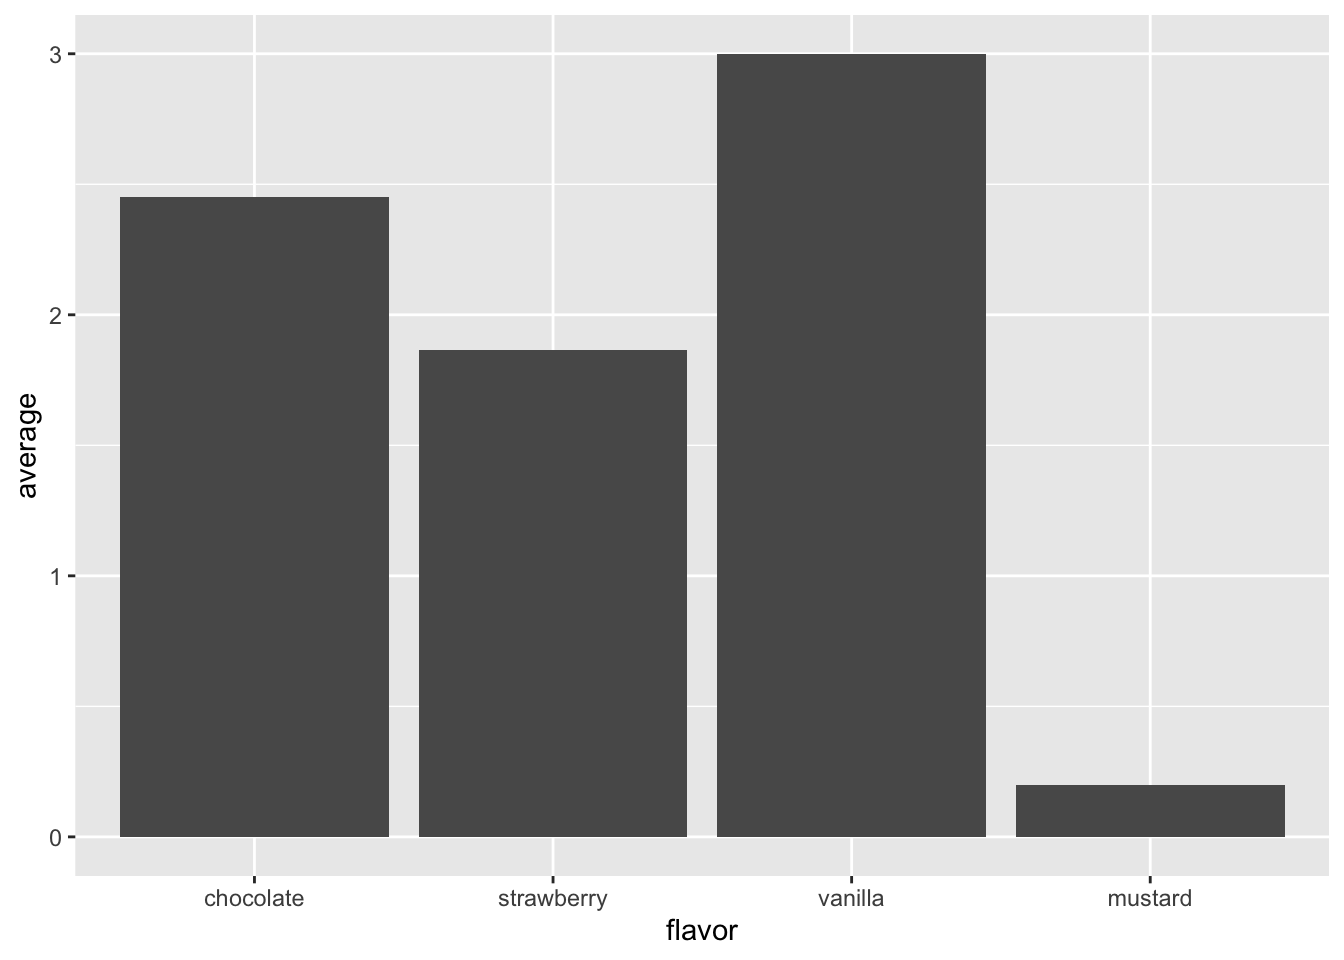
\includegraphics{debt_files/figure-latex/simple_bar_chart-1.pdf}

To learn more about how factors work and how to use them when analyzing categorical data,
please see \href{https://peerj.com/preprints/3163/}{this paper} by McNamara and Horton.

\hypertarget{how-do-i-refer-to-various-arguments-in-a-pipeline}{%
\section{How do I refer to various arguments in a pipeline?}\label{how-do-i-refer-to-various-arguments-in-a-pipeline}}

When we put a function in a pipeline using \texttt{\%\textgreater{}\%},
that operator calls the function with the incoming data as the first argument,
so \texttt{data\ \%\textgreater{}\%\ func(arg)} is the same as \texttt{func(data,\ arg)}.
This is fine when we want the incoming data to be the first argument,
but what if we want it to be second? Or third?

One possibility is to save the result so far in a temporary variable
and then start a second pipe:

\begin{Shaded}
\begin{Highlighting}[]
\NormalTok{data <-}\StringTok{ }\KeywordTok{tribble}\NormalTok{(}
  \OperatorTok{~}\NormalTok{left, }\OperatorTok{~}\NormalTok{right,}
  \DecValTok{1}\NormalTok{,     }\OtherTok{NA}\NormalTok{,}
  \DecValTok{2}\NormalTok{,     }\DecValTok{20}
\NormalTok{)}

\NormalTok{empties <-}\StringTok{ }\NormalTok{data }\OperatorTok
\StringTok{  }\KeywordTok{pmap_lgl}\NormalTok{(}\ControlFlowTok{function}\NormalTok{(...) \{}
\NormalTok{    args <-}\StringTok{ }\KeywordTok{list}\NormalTok{(...)}
    \KeywordTok{any}\NormalTok{(}\KeywordTok{is.na}\NormalTok{(args))}
\NormalTok{  \})}

\NormalTok{data }\OperatorTok
\StringTok{  }\KeywordTok{transmute}\NormalTok{(}\DataTypeTok{id =} \KeywordTok{row_number}\NormalTok{()) }\OperatorTok
\StringTok{  }\KeywordTok{filter}\NormalTok{(empties) }\OperatorTok
\StringTok{  }\KeywordTok{pull}\NormalTok{(id)}
\end{Highlighting}
\end{Shaded}

\begin{verbatim}
[1] 1
\end{verbatim}

This builds a logical vector \texttt{empties} with as many entries as \texttt{data} has rows,
then filters data according to which of the entries in the vector are \texttt{TRUE}.

A better practice is to use the parameter name \texttt{.},
which means ``the incoming data''.
In some functions (e.g., a two-argument function being used in \texttt{map})
we can also use \texttt{.x} and \texttt{.y} for the first and second arguments,
and for more arguments,
we can use \texttt{..1}, \texttt{..2}, and so on (with two dots at the front):

\begin{Shaded}
\begin{Highlighting}[]
\NormalTok{data }\OperatorTok
\StringTok{  }\KeywordTok{pmap_lgl}\NormalTok{(}\ControlFlowTok{function}\NormalTok{(...) \{}
\NormalTok{    args <-}\StringTok{ }\KeywordTok{list}\NormalTok{(...)}
    \KeywordTok{any}\NormalTok{(}\KeywordTok{is.na}\NormalTok{(args))}
\NormalTok{  \}) }\OperatorTok
\StringTok{  }\KeywordTok{tibble}\NormalTok{(}\DataTypeTok{empty =}\NormalTok{ .) }\OperatorTok
\StringTok{  }\KeywordTok{mutate}\NormalTok{(}\DataTypeTok{id =} \KeywordTok{row_number}\NormalTok{()) }\OperatorTok
\StringTok{  }\KeywordTok{filter}\NormalTok{(empty) }\OperatorTok
\StringTok{  }\KeywordTok{pull}\NormalTok{(id)}
\end{Highlighting}
\end{Shaded}

\begin{verbatim}
[1] 1
\end{verbatim}

In this model,
we create the logical vector,
then turn it into a tibble with one column called \texttt{empty}
(which is what \texttt{empty\ =\ .} does in \texttt{tibble}'s constructor).
After that,
we add another column with row numbers,
filter,
and pull out the row numbers.

And while we're here:
\texttt{row\_number} doesn't do what its name suggests.
We're better off using \texttt{rowid\_to\_column}:

\begin{Shaded}
\begin{Highlighting}[]
\NormalTok{data }\OperatorTok
\StringTok{  }\KeywordTok{rowid_to_column}\NormalTok{()}
\end{Highlighting}
\end{Shaded}

\begin{verbatim}
# A tibble: 2 x 3
  rowid  left right
  <int> <dbl> <dbl>
1     1     1    NA
2     2     2    20
\end{verbatim}

\hypertarget{i-thought-you-said-that-r-encouraged-functional-programming}{%
\section{I thought you said that R encouraged functional programming?}\label{i-thought-you-said-that-r-encouraged-functional-programming}}

I did.
Here is a function that reads a file and returns one of its columns:

\begin{Shaded}
\begin{Highlighting}[]
\NormalTok{col_from_file <-}\StringTok{ }\ControlFlowTok{function}\NormalTok{(filename, colname) \{}
\NormalTok{  dat <-}\StringTok{ }\NormalTok{readr}\OperatorTok{::}\KeywordTok{read_csv}\NormalTok{(filename)}
\NormalTok{  dat[colname]}
\NormalTok{\}}

\NormalTok{person_filename <-}\StringTok{ }\NormalTok{here}\OperatorTok{::}\KeywordTok{here}\NormalTok{(}\StringTok{"data"}\NormalTok{, }\StringTok{"person.csv"}\NormalTok{)}
\KeywordTok{col_from_file}\NormalTok{(person_filename, }\StringTok{"family_name"}\NormalTok{)}
\end{Highlighting}
\end{Shaded}

\begin{verbatim}
# A tibble: 5 x 1
  family_name
  <chr>      
1 Dyer       
2 Pabodie    
3 Lake       
4 Roerich    
5 Danforth   
\end{verbatim}

Note that the column name \emph{must} be passed as a quoted string;
Chapter~\ref{nse} will show us how to pass unquoted column names.

We might occasionally want to allow the user to specify
what values in the file are to be considered NAs.
This small addition allows us to do that,
while keeping the empty string and the string \texttt{"NA"} as defaults:

\begin{Shaded}
\begin{Highlighting}[]
\NormalTok{col_from_file <-}\StringTok{ }\ControlFlowTok{function}\NormalTok{(filename, colname, }\DataTypeTok{na =} \KeywordTok{c}\NormalTok{(}\StringTok{""}\NormalTok{, }\StringTok{"NA"}\NormalTok{)) \{}
\NormalTok{  dat <-}\StringTok{ }\NormalTok{readr}\OperatorTok{::}\KeywordTok{read_csv}\NormalTok{(filename, }\DataTypeTok{na =}\NormalTok{ na)}
\NormalTok{  dat[colname]}
\NormalTok{\}}

\KeywordTok{col_from_file}\NormalTok{(person_filename, }\StringTok{"family_name"}\NormalTok{, }\KeywordTok{c}\NormalTok{(}\StringTok{"Dyer"}\NormalTok{))}
\end{Highlighting}
\end{Shaded}

\begin{verbatim}
# A tibble: 5 x 1
  family_name
  <chr>      
1 <NA>       
2 Pabodie    
3 Lake       
4 Roerich    
5 Danforth   
\end{verbatim}

We can also allow the user to specify any number of columns
by capturing ``extra'' parameters in \texttt{...}
and passing that value directly to \texttt{dplyr::select}:

\begin{Shaded}
\begin{Highlighting}[]
\NormalTok{cols_from_file <-}\StringTok{ }\ControlFlowTok{function}\NormalTok{(filename, ..., }\DataTypeTok{na =} \KeywordTok{c}\NormalTok{(}\StringTok{""}\NormalTok{, }\StringTok{"NA"}\NormalTok{)) \{}
\NormalTok{  readr}\OperatorTok{::}\KeywordTok{read_csv}\NormalTok{(filename, }\DataTypeTok{na =}\NormalTok{ na) }\OperatorTok
\StringTok{    }\NormalTok{dplyr}\OperatorTok{::}\KeywordTok{select}\NormalTok{(...)}
\NormalTok{\}}

\KeywordTok{cols_from_file}\NormalTok{(person_filename, personal_name, family_name)}
\end{Highlighting}
\end{Shaded}

\begin{verbatim}
# A tibble: 5 x 2
  personal_name family_name
  <chr>         <chr>      
1 William       Dyer       
2 Frank         Pabodie    
3 Anderson      Lake       
4 Valentina     Roerich    
5 Frank         Danforth   
\end{verbatim}

Now that we can create functions,
we can use the tools in the \texttt{purrr} library to wield them.
\texttt{purrr::map} applies a function to each value in a vector in turn
and returns a list:

\begin{Shaded}
\begin{Highlighting}[]
\NormalTok{is_long_name <-}\StringTok{ }\ControlFlowTok{function}\NormalTok{(name) \{}
\NormalTok{  stringr}\OperatorTok{::}\KeywordTok{str_length}\NormalTok{(name) }\OperatorTok{>}\StringTok{ }\DecValTok{4}
\NormalTok{\}}

\NormalTok{person <-}\StringTok{ }\KeywordTok{read_csv}\NormalTok{(here}\OperatorTok{::}\KeywordTok{here}\NormalTok{(}\StringTok{"data"}\NormalTok{, }\StringTok{"person.csv"}\NormalTok{))}
\end{Highlighting}
\end{Shaded}

\begin{verbatim}
Parsed with column specification:
cols(
  person_id = col_character(),
  personal_name = col_character(),
  family_name = col_character()
)
\end{verbatim}

\begin{Shaded}
\begin{Highlighting}[]
\NormalTok{purrr}\OperatorTok{::}\KeywordTok{map}\NormalTok{(person}\OperatorTok{$}\NormalTok{family_name, is_long_name)}
\end{Highlighting}
\end{Shaded}

\begin{verbatim}
[[1]]
[1] FALSE

[[2]]
[1] TRUE

[[3]]
[1] FALSE

[[4]]
[1] TRUE

[[5]]
[1] TRUE
\end{verbatim}

For small calculations,
we will define the function where it is used---this is sometimes called
an \href{glossary.html\#anonymous-function}{anonymous function}
since it isn't given a name.
We will also use \texttt{purrr::map\_lgl}
so that the result of the call is a logical vector rather than a list.
Similarly-named functions will give us numbers, character strings, and so on:

\begin{Shaded}
\begin{Highlighting}[]
\NormalTok{purrr}\OperatorTok{::}\KeywordTok{map_lgl}\NormalTok{(person}\OperatorTok{$}\NormalTok{family_name,}
               \ControlFlowTok{function}\NormalTok{(name) stringr}\OperatorTok{::}\KeywordTok{str_length}\NormalTok{(name) }\OperatorTok{>}\StringTok{ }\DecValTok{4}\NormalTok{)}
\end{Highlighting}
\end{Shaded}

\begin{verbatim}
[1] FALSE  TRUE FALSE  TRUE  TRUE
\end{verbatim}

Little functions like this are so common
that \texttt{purrr} allows us to use write them as formulas using the \texttt{\textasciitilde{}\ operator\ with}.x` as a shorthand for the value from the vector being processed:

\begin{Shaded}
\begin{Highlighting}[]
\NormalTok{purrr}\OperatorTok{::}\KeywordTok{map_chr}\NormalTok{(person}\OperatorTok{$}\NormalTok{family_name, }\OperatorTok{~}\StringTok{ }\NormalTok{stringr}\OperatorTok{::}\KeywordTok{str_to_upper}\NormalTok{(.x))}
\end{Highlighting}
\end{Shaded}

\begin{verbatim}
[1] "DYER"     "PABODIE"  "LAKE"     "ROERICH"  "DANFORTH"
\end{verbatim}

Other functions in \texttt{purrr} let us work on two vectors at once:

\begin{Shaded}
\begin{Highlighting}[]
\NormalTok{purrr}\OperatorTok{::}\KeywordTok{map2_chr}\NormalTok{(person}\OperatorTok{$}\NormalTok{personal_name,}
\NormalTok{                person}\OperatorTok{$}\NormalTok{family_name,}
                \OperatorTok{~}\StringTok{ }\NormalTok{stringr}\OperatorTok{::}\KeywordTok{str_c}\NormalTok{(.y, .x, }\DataTypeTok{sep =} \StringTok{'_'}\NormalTok{))}
\end{Highlighting}
\end{Shaded}

\begin{verbatim}
[1] "Dyer_William"      "Pabodie_Frank"     "Lake_Anderson"    
[4] "Roerich_Valentina" "Danforth_Frank"   
\end{verbatim}

If we need to collapse the result to a single value
(e.g., to use in \texttt{if})
we have \texttt{purrr::some} and \texttt{purrr::every}:

\begin{Shaded}
\begin{Highlighting}[]
\NormalTok{purrr}\OperatorTok{::}\KeywordTok{every}\NormalTok{(person}\OperatorTok{$}\NormalTok{personal_name, }\OperatorTok{~}\StringTok{ }\NormalTok{.x }\OperatorTok{>}\StringTok{ 'M'}\NormalTok{)}
\end{Highlighting}
\end{Shaded}

\begin{verbatim}
[1] FALSE
\end{verbatim}

\hypertarget{modify-specific-elements-of-a-list}{%
\subsection{Modify specific elements of a list:}\label{modify-specific-elements-of-a-list}}

\begin{Shaded}
\begin{Highlighting}[]
\NormalTok{purrr}\OperatorTok{::}\KeywordTok{modify_at}\NormalTok{(person}\OperatorTok{$}\NormalTok{personal_name, }\KeywordTok{c}\NormalTok{(}\DecValTok{2}\NormalTok{, }\DecValTok{4}\NormalTok{), stringr}\OperatorTok{::}\NormalTok{str_to_upper)}
\end{Highlighting}
\end{Shaded}

\begin{verbatim}
[1] "William"   "FRANK"     "Anderson"  "VALENTINA" "Frank"    
\end{verbatim}

\emph{Use \texttt{modify\_if} to upper-case names that are greater than ``M''.}

\hypertarget{create-an-acronym}{%
\subsection{Create an acronym:}\label{create-an-acronym}}

\begin{Shaded}
\begin{Highlighting}[]
\NormalTok{purrr}\OperatorTok{::}\KeywordTok{reduce}\NormalTok{(person}\OperatorTok{$}\NormalTok{personal_name, }\OperatorTok{~}\NormalTok{stringr}\OperatorTok{::}\KeywordTok{str_c}\NormalTok{(.x, stringr}\OperatorTok{::}\KeywordTok{str_sub}\NormalTok{(.y, }\DecValTok{1}\NormalTok{, }\DecValTok{1}\NormalTok{)), }\DataTypeTok{.init =} \StringTok{""}\NormalTok{)}
\end{Highlighting}
\end{Shaded}

\begin{verbatim}
[1] "WFAVF"
\end{verbatim}

\emph{Explain why using \texttt{stringr::str\_c(stringr::str\_sub(.x,\ 1,\ 1),\ stringr::str\_sub(.y,\ 1,\ 1))} doesn't work.}

\hypertarget{create-intermediate-values}{%
\subsection{Create intermediate values:}\label{create-intermediate-values}}

\begin{Shaded}
\begin{Highlighting}[]
\NormalTok{purrr}\OperatorTok{::}\KeywordTok{accumulate}\NormalTok{(person}\OperatorTok{$}\NormalTok{personal_name, }\OperatorTok{~}\NormalTok{stringr}\OperatorTok{::}\KeywordTok{str_c}\NormalTok{(.x, stringr}\OperatorTok{::}\KeywordTok{str_sub}\NormalTok{(.y, }\DecValTok{1}\NormalTok{, }\DecValTok{1}\NormalTok{)), }\DataTypeTok{.init =} \StringTok{""}\NormalTok{)}
\end{Highlighting}
\end{Shaded}

\begin{verbatim}
[1] ""      "W"     "WF"    "WFA"   "WFAV"  "WFAVF"
\end{verbatim}

\emph{Modify this so that the initial empty string isn't in the final result.}

\hypertarget{how-does-r-give-the-appearance-of-immutable-data}{%
\section{How does R give the appearance of immutable data?}\label{how-does-r-give-the-appearance-of-immutable-data}}

Another feature of R that can surprise the unwary is its use of \href{glossary.html\#copy-on-modify}{copy-on-modify}
to make data appear \href{glossary.html\#immutable}{immutable}
(a jargon term meaning ``cannot be changed after creation'').
If two or more variables refer to the same data
and that data is updated via one variable,
R automatically makes a copy of the data so that the other variable's value doesn't change.
Here's a simple example:

\begin{Shaded}
\begin{Highlighting}[]
\NormalTok{first <-}\StringTok{ }\KeywordTok{c}\NormalTok{(}\StringTok{"red"}\NormalTok{, }\StringTok{"green"}\NormalTok{, }\StringTok{"blue"}\NormalTok{)}
\NormalTok{second <-}\StringTok{ }\NormalTok{first}
\KeywordTok{print}\NormalTok{(}\KeywordTok{glue}\NormalTok{(}\StringTok{"before modification, first is \{paste(first, collapse='-')\} and second is \{paste(second, collapse='-')\}"}\NormalTok{))}
\end{Highlighting}
\end{Shaded}

\begin{verbatim}
before modification, first is red-green-blue and second is red-green-blue
\end{verbatim}

\begin{Shaded}
\begin{Highlighting}[]
\NormalTok{first[[}\DecValTok{1}\NormalTok{]] <-}\StringTok{ "sulphurous"}
\KeywordTok{print}\NormalTok{(}\KeywordTok{glue}\NormalTok{(}\StringTok{"after modification, first is \{paste(first, collapse='-')\} and second is \{paste(second, collapse='-')\}"}\NormalTok{))}
\end{Highlighting}
\end{Shaded}

\begin{verbatim}
after modification, first is sulphurous-green-blue and second is red-green-blue
\end{verbatim}

This is true of nested structures as well:

\begin{Shaded}
\begin{Highlighting}[]
\NormalTok{first <-}\StringTok{ }\KeywordTok{tribble}\NormalTok{(}
  \OperatorTok{~}\NormalTok{left, }\OperatorTok{~}\NormalTok{right,}
  \DecValTok{101}\NormalTok{,   }\DecValTok{202}\NormalTok{,}
  \DecValTok{303}\NormalTok{,   }\DecValTok{404}\NormalTok{)}
\NormalTok{second <-}\StringTok{ }\NormalTok{first}
\NormalTok{first}\OperatorTok{$}\NormalTok{left[[}\DecValTok{1}\NormalTok{]] <-}\StringTok{ }\DecValTok{999}
\KeywordTok{print}\NormalTok{(}\StringTok{"first after modification"}\NormalTok{)}
\end{Highlighting}
\end{Shaded}

\begin{verbatim}
[1] "first after modification"
\end{verbatim}

\begin{Shaded}
\begin{Highlighting}[]
\NormalTok{first}
\end{Highlighting}
\end{Shaded}

\begin{verbatim}
# A tibble: 2 x 2
   left right
  <dbl> <dbl>
1   999   202
2   303   404
\end{verbatim}

\begin{Shaded}
\begin{Highlighting}[]
\KeywordTok{print}\NormalTok{(}\StringTok{"second after modification"}\NormalTok{)}
\end{Highlighting}
\end{Shaded}

\begin{verbatim}
[1] "second after modification"
\end{verbatim}

\begin{Shaded}
\begin{Highlighting}[]
\NormalTok{second}
\end{Highlighting}
\end{Shaded}

\begin{verbatim}
# A tibble: 2 x 2
   left right
  <dbl> <dbl>
1   101   202
2   303   404
\end{verbatim}

In this case,
the entire \texttt{left} column of \texttt{first} has been replaced:
tibbles (and data frames) are stored as lists of vectors,
so changing any value in a column triggers construction of a new column vector.

We can watch this happen using the \texttt{tracemem} function,
which shows us where objects live in the computer's memory:

\begin{Shaded}
\begin{Highlighting}[]
\NormalTok{first <-}\StringTok{ }\KeywordTok{tribble}\NormalTok{(}
  \OperatorTok{~}\NormalTok{left, }\OperatorTok{~}\NormalTok{right,}
  \DecValTok{101}\NormalTok{,   }\DecValTok{202}\NormalTok{,}
  \DecValTok{303}\NormalTok{,   }\DecValTok{404}
\NormalTok{)}
\KeywordTok{tracemem}\NormalTok{(first)}
\end{Highlighting}
\end{Shaded}

\begin{verbatim}
[1] "<0x7f9c079daa48>"
\end{verbatim}

\begin{Shaded}
\begin{Highlighting}[]
\NormalTok{first}\OperatorTok{$}\NormalTok{left[[}\DecValTok{1}\NormalTok{]] <-}\StringTok{ }\DecValTok{999}
\end{Highlighting}
\end{Shaded}

\begin{verbatim}
tracemem[0x7f9c079daa48 -> 0x7f9c0794fb88]: eval eval withVisible withCallingHandlers handle timing_fn evaluate_call <Anonymous> evaluate in_dir block_exec call_block process_group.block process_group withCallingHandlers process_file <Anonymous> <Anonymous> do.call eval eval eval eval eval.parent local 
tracemem[0x7f9c0794fb88 -> 0x7f9c0794fc08]: eval eval withVisible withCallingHandlers handle timing_fn evaluate_call <Anonymous> evaluate in_dir block_exec call_block process_group.block process_group withCallingHandlers process_file <Anonymous> <Anonymous> do.call eval eval eval eval eval.parent local 
tracemem[0x7f9c0794fc08 -> 0x7f9c0794fc88]: $<-.data.frame $<- eval eval withVisible withCallingHandlers handle timing_fn evaluate_call <Anonymous> evaluate in_dir block_exec call_block process_group.block process_group withCallingHandlers process_file <Anonymous> <Anonymous> do.call eval eval eval eval eval.parent local 
tracemem[0x7f9c0794fc88 -> 0x7f9c0794fcc8]: $<-.data.frame $<- eval eval withVisible withCallingHandlers handle timing_fn evaluate_call <Anonymous> evaluate in_dir block_exec call_block process_group.block process_group withCallingHandlers process_file <Anonymous> <Anonymous> do.call eval eval eval eval eval.parent local 
\end{verbatim}

\begin{Shaded}
\begin{Highlighting}[]
\KeywordTok{untracemem}\NormalTok{(first)}
\end{Highlighting}
\end{Shaded}

This rather cryptic output tell us the address of the tibble,
then notifies us of changes to the tibble and its contents.
We can accomplish something a little more readable using \texttt{pryr::address}
(i.e., the \texttt{address} function from the pryr package):

\begin{Shaded}
\begin{Highlighting}[]
\NormalTok{left <-}\StringTok{ }\NormalTok{first}\OperatorTok{$}\NormalTok{left }\CommentTok{# alias}
\KeywordTok{print}\NormalTok{(}\KeywordTok{glue}\NormalTok{(}\StringTok{"left column is initially at \{pryr::address(left)\}"}\NormalTok{))}
\end{Highlighting}
\end{Shaded}

\begin{verbatim}
Registered S3 method overwritten by 'pryr':
  method      from
  print.bytes Rcpp
\end{verbatim}

\begin{verbatim}
left column is initially at 0x7f9c0794fbc8
\end{verbatim}

\begin{Shaded}
\begin{Highlighting}[]
\NormalTok{first}\OperatorTok{$}\NormalTok{left[[}\DecValTok{2}\NormalTok{]] <-}\StringTok{ }\DecValTok{888}
\KeywordTok{print}\NormalTok{(}\KeywordTok{glue}\NormalTok{(}\StringTok{"after modification, the original column is still at \{pryr::address(left)\}"}\NormalTok{))}
\end{Highlighting}
\end{Shaded}

\begin{verbatim}
after modification, the original column is still at 0x7f9c0794fbc8
\end{verbatim}

\begin{Shaded}
\begin{Highlighting}[]
\NormalTok{temp <-}\StringTok{ }\NormalTok{first}\OperatorTok{$}\NormalTok{left }\CommentTok{# another alias}
\KeywordTok{print}\NormalTok{(}\KeywordTok{glue}\NormalTok{(}\StringTok{"but the first column is at \{pryr::address(temp)\}"}\NormalTok{))}
\end{Highlighting}
\end{Shaded}

\begin{verbatim}
but the first column is at 0x7f9c037351c8
\end{verbatim}

(We need to use the \href{glossary.html\#alias}{alias} \texttt{temp} because \texttt{address(first\$left)} doesn't work:
the argument to \texttt{address} needs to be a variable name.)

R's copy-on-modify semantics is particularly important when writing functions.
If we modify an argument inside a function,
that modification isn't visible to the caller,
so even functions that appear to modify structures usually don't.
(``Usually'', because there are exceptions, but we must stray off the path to find them.)

\hypertarget{what-else-should-i-worry-about}{%
\section{What else should I worry about?}\label{what-else-should-i-worry-about}}

Ralph Waldo Emerson once wrote, ``A foolish consistency is the hobgoblin of little minds.''
Here, then, are few of the hobgoblins I've encountered on my journey through R.

\hypertarget{the-order-function}{%
\subsection{\texorpdfstring{The \texttt{order} function}{The order function}}\label{the-order-function}}

The function \texttt{order} generates indices to pull values into place rather than push them,
i.e.,
\texttt{order(x){[}i{]}} is the index in \texttt{x} of the element that belongs at location \texttt{i}.
For example:

\begin{Shaded}
\begin{Highlighting}[]
\NormalTok{bases <-}\StringTok{ }\KeywordTok{c}\NormalTok{(}\StringTok{"g"}\NormalTok{, }\StringTok{"c"}\NormalTok{, }\StringTok{"t"}\NormalTok{, }\StringTok{"a"}\NormalTok{)}
\KeywordTok{order}\NormalTok{(bases)}
\end{Highlighting}
\end{Shaded}

\begin{verbatim}
[1] 4 2 1 3
\end{verbatim}

shows that the value at location 4 (the \texttt{"a"}) belongs in the first spot of the vector;
it does \emph{not} mean that the value in the first location (the \texttt{"g"}) belongs in location 4.
This convention means that \texttt{something{[}order(something){]}} does the right thing:

\begin{Shaded}
\begin{Highlighting}[]
\NormalTok{bases[}\KeywordTok{order}\NormalTok{(bases)]}
\end{Highlighting}
\end{Shaded}

\begin{verbatim}
[1] "a" "c" "g" "t"
\end{verbatim}

\hypertarget{one-of-a-set-of-values}{%
\subsection{One of a set of values}\label{one-of-a-set-of-values}}

The function \texttt{one\_of} is a handy way to specify several values for matching
without complicated Boolean conditionals.
For example,
\texttt{gather(data,\ key\ =\ "year",\ value\ =\ "cases",\ one\_of(c("1999",\ "2000")))}
collects data for the years 1999 and 2000.

\hypertarget{and-are-not-the-same-as-and}{%
\subsection{\texorpdfstring{\texttt{\textbar{}} and \texttt{\&} are not the same as \texttt{\textbar{}\textbar{}} and \texttt{\&\&}}{\textbar{} and \& are not the same as \textbar{}\textbar{} and \&\&}}\label{and-are-not-the-same-as-and}}

Let's try some experiments:

\begin{Shaded}
\begin{Highlighting}[]
\NormalTok{TRUE_TRUE <-}\StringTok{ }\KeywordTok{c}\NormalTok{(}\OtherTok{TRUE}\NormalTok{, }\OtherTok{TRUE}\NormalTok{)}
\NormalTok{TRUE_FALSE <-}\StringTok{ }\KeywordTok{c}\NormalTok{(}\OtherTok{TRUE}\NormalTok{, }\OtherTok{FALSE}\NormalTok{)}
\NormalTok{FALSE_TRUE <-}\StringTok{ }\KeywordTok{c}\NormalTok{(}\OtherTok{FALSE}\NormalTok{, }\OtherTok{TRUE}\NormalTok{)}
\KeywordTok{print}\NormalTok{(}\KeywordTok{glue}\NormalTok{(}\StringTok{"TRUE_TRUE &  TRUE_FALSE: \{paste(TRUE_TRUE &  TRUE_FALSE, collapse = ' ')\}"}\NormalTok{))}
\end{Highlighting}
\end{Shaded}

\begin{verbatim}
TRUE_TRUE &  TRUE_FALSE: TRUE FALSE
\end{verbatim}

\begin{Shaded}
\begin{Highlighting}[]
\KeywordTok{print}\NormalTok{(}\KeywordTok{glue}\NormalTok{(}\StringTok{"TRUE_TRUE &  FALSE_TRUE: \{paste(TRUE_TRUE &  FALSE_TRUE, collapse = ' ')\}"}\NormalTok{))}
\end{Highlighting}
\end{Shaded}

\begin{verbatim}
TRUE_TRUE &  FALSE_TRUE: FALSE TRUE
\end{verbatim}

\begin{Shaded}
\begin{Highlighting}[]
\KeywordTok{print}\NormalTok{(}\KeywordTok{glue}\NormalTok{(}\StringTok{"TRUE_TRUE && TRUE_FALSE: \{paste(TRUE_TRUE && TRUE_FALSE, collapse = ' ')\}"}\NormalTok{))}
\end{Highlighting}
\end{Shaded}

\begin{verbatim}
TRUE_TRUE && TRUE_FALSE: TRUE
\end{verbatim}

\begin{Shaded}
\begin{Highlighting}[]
\KeywordTok{print}\NormalTok{(}\KeywordTok{glue}\NormalTok{(}\StringTok{"TRUE_TRUE && FALSE_TRUE: \{paste(TRUE_TRUE && FALSE_TRUE, collapse = ' ')\}"}\NormalTok{))}
\end{Highlighting}
\end{Shaded}

\begin{verbatim}
TRUE_TRUE && FALSE_TRUE: FALSE
\end{verbatim}

The difference is that \texttt{\&} always returns a vector result after doing element-by-element conjunction,
while \texttt{\&\&} returns a scalar result.
This means that \texttt{\&} is almost always what we want to use when working with data.

\hypertarget{functions-and-columns}{%
\subsection{Functions and columns}\label{functions-and-columns}}

There is a function called \texttt{n}.
It's not the same thing as a column called \texttt{n}.
I only made this mistake a dozen times.

\begin{Shaded}
\begin{Highlighting}[]
\NormalTok{data <-}\StringTok{ }\KeywordTok{tribble}\NormalTok{(}
  \OperatorTok{~}\NormalTok{a, }\OperatorTok{~}\NormalTok{n,}
  \DecValTok{1}\NormalTok{,  }\DecValTok{10}\NormalTok{,}
  \DecValTok{2}\NormalTok{,  }\DecValTok{20}
\NormalTok{)}
\NormalTok{data }\OperatorTok\StringTok{ }\KeywordTok{summarize}\NormalTok{(}\DataTypeTok{total =} \KeywordTok{sum}\NormalTok{(n))}
\end{Highlighting}
\end{Shaded}

\begin{verbatim}
# A tibble: 1 x 1
  total
  <dbl>
1    30
\end{verbatim}

\begin{Shaded}
\begin{Highlighting}[]
\NormalTok{data }\OperatorTok\StringTok{ }\KeywordTok{summarize}\NormalTok{(}\DataTypeTok{total =} \KeywordTok{sum}\NormalTok{(}\KeywordTok{n}\NormalTok{()))}
\end{Highlighting}
\end{Shaded}

\begin{verbatim}
# A tibble: 1 x 1
  total
  <int>
1     2
\end{verbatim}

\hypertarget{key-points-5}{%
\section{Key Points}\label{key-points-5}}

\begin{itemize}
\tightlist
\item
  Don't use \texttt{setwd}.
\item
  The formula operator \texttt{\textasciitilde{}} delays evaluation of its operand or operands.
\item
  \texttt{\textasciitilde{}} was created to allow users to pass formulas into functions, but is used more generally to delay evaluation.
\item
  Some tidyverse functions define \texttt{.} to be the whole data, \texttt{.x} and \texttt{.y} to be the first and second arguments, and \texttt{..N} to be the N'th argument.
\item
  These convenience parameters are primarily used when the data being passed to a pipelined function needs to go somewhere other than in the first parameter's slot.
\item
  `Copy-on-modify' means that data is aliased until something attempts to modify it, at which point it duplicated, so that data always appears to be unchanged.
\end{itemize}

\hypertarget{testerror}{%
\chapter{Testing and Error Handling}\label{testerror}}

Novices write code and pray that it works.
Experienced programmers know that prayer alone is not enough,
and take steps to protect what little sanity they have left.
This chapter looks at the tools R gives us for doing this.

\hypertarget{learning-objectives-6}{%
\section{Learning Objectives}\label{learning-objectives-6}}

\begin{itemize}
\tightlist
\item
  Name and describe the three levels of error handling in R.
\item
  Handle an otherwise-fatal error in a function call in R.
\item
  Create unit tests in R.
\item
  Create unit tests for an R package.
\end{itemize}

\hypertarget{how-does-r-handle-errors}{%
\section{How does R handle errors?}\label{how-does-r-handle-errors}}

Python programs handle errors
by \href{glossary.html\#raise-exception}{raising} and \href{glossary.html\#catch-exception}{catching} \href{glossary.html\#exception}{exceptions}:

\begin{Shaded}
\begin{Highlighting}[]
\NormalTok{values }\OperatorTok{=}\NormalTok{ [}\OperatorTok{-}\DecValTok{1}\NormalTok{, }\DecValTok{0}\NormalTok{, }\DecValTok{1}\NormalTok{]}
\ControlFlowTok{for}\NormalTok{ i }\KeywordTok{in} \BuiltInTok{range}\NormalTok{(}\DecValTok{4}\NormalTok{):}
    \ControlFlowTok{try}\NormalTok{:}
\NormalTok{        reciprocal }\OperatorTok{=} \DecValTok{1}\OperatorTok{/}\NormalTok{values[i]}
        \BuiltInTok{print}\NormalTok{(}\StringTok{"index }\SpecialCharTok{\{\}}\StringTok{ value }\SpecialCharTok{\{\}}\StringTok{ reciprocal }\SpecialCharTok{\{\}}\StringTok{"}\NormalTok{.}\BuiltInTok{format}\NormalTok{(i, values[i], reciprocal))}
    \ControlFlowTok{except} \PreprocessorTok{ZeroDivisionError}\NormalTok{:}
        \BuiltInTok{print}\NormalTok{(}\StringTok{"index }\SpecialCharTok{\{\}}\StringTok{ value }\SpecialCharTok{\{\}}\StringTok{ ZeroDivisionError"}\NormalTok{.}\BuiltInTok{format}\NormalTok{(i, values[i]))}
    \ControlFlowTok{except} \PreprocessorTok{Exception} \ImportTok{as}\NormalTok{ e:}
        \BuiltInTok{print}\NormalTok{(}\StringTok{"index}\SpecialCharTok{\{\}}\StringTok{ some other Exception: }\SpecialCharTok{\{\}}\StringTok{"}\NormalTok{.}\BuiltInTok{format}\NormalTok{(i, e))}
\end{Highlighting}
\end{Shaded}

\begin{verbatim}
index 0 value -1 reciprocal -1.0
index 1 value 0 ZeroDivisionError
index 2 value 1 reciprocal 1.0
index3 some other Exception: list index out of range
\end{verbatim}

R draws on a different tradition.
We say that the operation \href{glossary.html\#signal-condition}{signals} a \href{glossary.html\#condition}{condition}
that some other piece of code then \href{glossary.html\#handle-condition}{handles}.
These things are all simpler to do using the rlang library,
so we begin by loading that:

In order of increasing severity,
the three built-in kinds of conditions are \href{glossary.html\#message}{messages},
\href{glossary.html\#warning}{warnings},
and \href{glossary.html\#error}{errors}.
(There are also interrupts,
which are generated by the user pressing Ctrl-C to stop an operation,
but we will ignore those for the sake of brevity.)
We can signal conditions of these kinds using the functions \texttt{message}, \texttt{warning}, and \texttt{stop},
each of which takes an error message as a parameter:

\begin{Shaded}
\begin{Highlighting}[]
\KeywordTok{message}\NormalTok{(}\StringTok{"This is a message."}\NormalTok{)}
\end{Highlighting}
\end{Shaded}

\begin{verbatim}
This is a message.
\end{verbatim}

\begin{Shaded}
\begin{Highlighting}[]
\KeywordTok{warning}\NormalTok{(}\StringTok{"This is a warning.}\CharTok{\textbackslash{}n}\StringTok{"}\NormalTok{)}
\end{Highlighting}
\end{Shaded}

\begin{verbatim}
Warning: This is a warning.
\end{verbatim}

\begin{Shaded}
\begin{Highlighting}[]
\KeywordTok{stop}\NormalTok{(}\StringTok{"This is an error."}\NormalTok{)}
\end{Highlighting}
\end{Shaded}

\begin{verbatim}
Error in eval(expr, envir, enclos): This is an error.
\end{verbatim}

Note that we have to supply our own line ending for warnings
but not for the other two cases.
Note also that there are very few situations in which a warning is appropriate:
if something has truly gone wrong then we should stop,
but otherwise we should not distract users from more pressing concerns.

The bluntest of instruments for handling errors is to ignore them.
If a statement is wrapped in the function \texttt{try}
then errors that occur in it are still reported,
but execution continues.
Compare this:

\begin{Shaded}
\begin{Highlighting}[]
\NormalTok{attemptWithoutTry <-}\StringTok{ }\ControlFlowTok{function}\NormalTok{(left, right)\{}
\NormalTok{  temp <-}\StringTok{ }\NormalTok{left }\OperatorTok{+}\StringTok{ }\NormalTok{right}
  \StringTok{"result"} \CommentTok{# returned}
\NormalTok{\}}
\NormalTok{result <-}\StringTok{ }\KeywordTok{attemptWithoutTry}\NormalTok{(}\DecValTok{1}\NormalTok{, }\StringTok{"two"}\NormalTok{)}
\end{Highlighting}
\end{Shaded}

\begin{verbatim}
Error in left + right: non-numeric argument to binary operator
\end{verbatim}

\begin{Shaded}
\begin{Highlighting}[]
\KeywordTok{cat}\NormalTok{(}\StringTok{"result is"}\NormalTok{, result)}
\end{Highlighting}
\end{Shaded}

\begin{verbatim}
Error in cat("result is", result): object 'result' not found
\end{verbatim}

with this:

\begin{Shaded}
\begin{Highlighting}[]
\NormalTok{attemptUsingTry <-}\StringTok{ }\ControlFlowTok{function}\NormalTok{(left, right)\{}
\NormalTok{  temp <-}\StringTok{ }\KeywordTok{try}\NormalTok{(left }\OperatorTok{+}\StringTok{ }\NormalTok{right)}
  \StringTok{"value returned"} \CommentTok{# returned}
\NormalTok{\}}
\NormalTok{result <-}\StringTok{ }\KeywordTok{attemptUsingTry}\NormalTok{(}\DecValTok{1}\NormalTok{, }\StringTok{"two"}\NormalTok{)}
\end{Highlighting}
\end{Shaded}

\begin{verbatim}
Error in left + right : non-numeric argument to binary operator
\end{verbatim}

\begin{Shaded}
\begin{Highlighting}[]
\KeywordTok{cat}\NormalTok{(}\StringTok{"result is"}\NormalTok{, result)}
\end{Highlighting}
\end{Shaded}

\begin{verbatim}
result is value returned
\end{verbatim}

We can suppress error messages from \texttt{try} by setting \texttt{silent} to \texttt{TRUE}:

\begin{Shaded}
\begin{Highlighting}[]
\NormalTok{attemptUsingTryQuietly <-}\StringTok{ }\ControlFlowTok{function}\NormalTok{(left, right)\{}
\NormalTok{  temp <-}\StringTok{ }\KeywordTok{try}\NormalTok{(left }\OperatorTok{+}\StringTok{ }\NormalTok{right, }\DataTypeTok{silent =} \OtherTok{TRUE}\NormalTok{)}
  \StringTok{"result"} \CommentTok{# returned}
\NormalTok{\}}
\NormalTok{result <-}\StringTok{ }\KeywordTok{attemptUsingTryQuietly}\NormalTok{(}\DecValTok{1}\NormalTok{, }\StringTok{"two"}\NormalTok{)}
\KeywordTok{cat}\NormalTok{(}\StringTok{"result is"}\NormalTok{, result)}
\end{Highlighting}
\end{Shaded}

\begin{verbatim}
result is result
\end{verbatim}

Do not do this,
lest you one day find yourself lost in a silent hellscape.

Should you more sensibly wish to handle conditions rather than ignore them,
you may invoke \texttt{tryCatch}.
We begin by raising an error explicitly:

\begin{Shaded}
\begin{Highlighting}[]
\KeywordTok{tryCatch}\NormalTok{(}
  \KeywordTok{stop}\NormalTok{(}\StringTok{"our message"}\NormalTok{),}
  \DataTypeTok{error =} \ControlFlowTok{function}\NormalTok{(cnd) }\KeywordTok{print}\NormalTok{(}\KeywordTok{glue}\NormalTok{(}\StringTok{"error object is \{cnd\}"}\NormalTok{))}
\NormalTok{)}
\end{Highlighting}
\end{Shaded}

\begin{verbatim}
error object is Error in doTryCatch(return(expr), name, parentenv, handler): our message
\end{verbatim}

We can now run a function that would otherwise blow up:

\begin{Shaded}
\begin{Highlighting}[]
\KeywordTok{tryCatch}\NormalTok{(}
  \KeywordTok{attemptWithoutTry}\NormalTok{(}\DecValTok{1}\NormalTok{, }\StringTok{"two"}\NormalTok{),}
  \DataTypeTok{error =} \ControlFlowTok{function}\NormalTok{(cnd) }\KeywordTok{print}\NormalTok{(}\KeywordTok{glue}\NormalTok{(}\StringTok{"error object is \{cnd\}"}\NormalTok{))}
\NormalTok{)}
\end{Highlighting}
\end{Shaded}

\begin{verbatim}
error object is Error in left + right: non-numeric argument to binary operator
\end{verbatim}

We can also handle non-fatal errors using \texttt{withCallingHandlers},
and define new types of conditions,
but this is done less often in day-to-day R code than in Python:
see \emph{\href{http://adv-r.had.co.nz/}{Advanced R}} or \href{https://www.onceupondata.com/2018/09/28/handling-r-errors/}{this tutorial} for details.

\hypertarget{what-should-i-know-about-testing-in-general}{%
\section{What should I know about testing in general?}\label{what-should-i-know-about-testing-in-general}}

In keeping with common programming practice,
we have left testing until the last possible moment.
The standard testing library for R is \href{https://github.com/r-lib/testthat}{testthat},
which shares many features with Python's \href{https://docs.python.org/3/library/unittest.html}{unittest}
and other \href{glossary.html\#unit-test}{unit testing} libraries:

\begin{enumerate}
\def\labelenumi{\arabic{enumi}.}
\tightlist
\item
  Each test consists of a single function that tests a single property or behavior of the system.
\item
  Tests are collected into files with prescribed names that can be found by a \href{glossary.html\#test-runner}{test runner}.
\item
  Shared \href{glossary.html\#testing-setup}{setup} and \href{glossary.html\#testing-teardown}{teardown} steps are put in functions of their own.
\end{enumerate}

Let's load it and write our first test:

\begin{Shaded}
\begin{Highlighting}[]
\KeywordTok{library}\NormalTok{(testthat)}
\end{Highlighting}
\end{Shaded}

\begin{verbatim}

Attaching package: 'testthat'
\end{verbatim}

\begin{verbatim}
The following objects are masked from 'package:rlang':

    is_false, is_null, is_true
\end{verbatim}

\begin{verbatim}
The following object is masked from 'package:dplyr':

    matches
\end{verbatim}

\begin{verbatim}
The following object is masked from 'package:purrr':

    is_null
\end{verbatim}

\begin{verbatim}
The following object is masked from 'package:tidyr':

    matches
\end{verbatim}

\begin{Shaded}
\begin{Highlighting}[]
\KeywordTok{test_that}\NormalTok{(}\StringTok{"Zero equals itself"}\NormalTok{, \{}\KeywordTok{expect_equal}\NormalTok{(}\DecValTok{0}\NormalTok{, }\DecValTok{0}\NormalTok{)\})}
\end{Highlighting}
\end{Shaded}

As is conventional with unit testing libraries,
no news is good news:
if a test passes,
it doesn't produce output because it doesn't need our attention.
Let's try something that ought to fail:

\begin{Shaded}
\begin{Highlighting}[]
\KeywordTok{test_that}\NormalTok{(}\StringTok{"Zero equals one"}\NormalTok{, \{}\KeywordTok{expect_equal}\NormalTok{(}\DecValTok{0}\NormalTok{, }\DecValTok{1}\NormalTok{)\})}
\end{Highlighting}
\end{Shaded}

\begin{verbatim}
Error: Test failed: 'Zero equals one'
* 0 not equal to 1.
1/1 mismatches
[1] 0 - 1 == -1
\end{verbatim}

Good:
we can draw some comfort from the fact that Those Beyond have not yet changed the fundamental rules of arithmetic.
But what are the curly braces around \texttt{expect\_equal} for?
The answer is that they create a \href{glossary.html\#code-block}{code block} for \texttt{test\_that} to run.
We can run \texttt{expect\_equal} on its own:

\begin{Shaded}
\begin{Highlighting}[]
\KeywordTok{expect_equal}\NormalTok{(}\DecValTok{0}\NormalTok{, }\DecValTok{1}\NormalTok{)}
\end{Highlighting}
\end{Shaded}

\begin{verbatim}
Error: 0 not equal to 1.
1/1 mismatches
[1] 0 - 1 == -1
\end{verbatim}

but that doesn't produce a summary of how many tests passed or failed.
Passing a block of code to \texttt{test\_that} also allows us to check several things in one test:

\begin{Shaded}
\begin{Highlighting}[]
\KeywordTok{test_that}\NormalTok{(}\StringTok{"Testing two things"}\NormalTok{, \{}
  \KeywordTok{expect_equal}\NormalTok{(}\DecValTok{0}\NormalTok{, }\DecValTok{0}\NormalTok{)}
  \KeywordTok{expect_equal}\NormalTok{(}\DecValTok{0}\NormalTok{, }\DecValTok{1}\NormalTok{)}
\NormalTok{\})}
\end{Highlighting}
\end{Shaded}

\begin{verbatim}
Error: Test failed: 'Testing two things'
* 0 not equal to 1.
1/1 mismatches
[1] 0 - 1 == -1
\end{verbatim}

A block of code is \emph{not} the same thing as an \href{glossary.html\#anonymous-function}{anonymous function},
which is why running this block of code does nothing---the ``test'' defines a function
but doesn't actually call it:

\begin{Shaded}
\begin{Highlighting}[]
\KeywordTok{test_that}\NormalTok{(}\StringTok{"Using an anonymous function"}\NormalTok{, }\ControlFlowTok{function}\NormalTok{() \{}
  \KeywordTok{print}\NormalTok{(}\StringTok{"In our anonymous function"}\NormalTok{)}
  \KeywordTok{expect_equal}\NormalTok{(}\DecValTok{0}\NormalTok{, }\DecValTok{1}\NormalTok{)}
\NormalTok{\})}
\end{Highlighting}
\end{Shaded}

\hypertarget{how-should-i-organize-my-tests}{%
\section{How should I organize my tests?}\label{how-should-i-organize-my-tests}}

Running blocks of tests by hand is a bad practice.
Instead,
we should put related tests in files
and then put those files in a directory called \texttt{tests/testthat}.
We can then run some or all of those tests with a single command.

To start,
let's create \texttt{tests/testthat/test\_example.R}:

\begin{Shaded}
\begin{Highlighting}[]
\KeywordTok{library}\NormalTok{(testthat)}
\KeywordTok{context}\NormalTok{(}\StringTok{"Demonstrating the testing library"}\NormalTok{)}

\KeywordTok{test_that}\NormalTok{(}\StringTok{"Testing a number with itself"}\NormalTok{, \{}
  \KeywordTok{expect_equal}\NormalTok{(}\DecValTok{0}\NormalTok{, }\DecValTok{0}\NormalTok{)}
  \KeywordTok{expect_equal}\NormalTok{(}\OperatorTok{-}\DecValTok{1}\NormalTok{, }\DecValTok{-1}\NormalTok{)}
  \KeywordTok{expect_equal}\NormalTok{(}\OtherTok{Inf}\NormalTok{, }\OtherTok{Inf}\NormalTok{)}
\NormalTok{\})}

\KeywordTok{test_that}\NormalTok{(}\StringTok{"Testing different numbers"}\NormalTok{, \{}
  \KeywordTok{expect_equal}\NormalTok{(}\DecValTok{0}\NormalTok{, }\DecValTok{1}\NormalTok{)}
\NormalTok{\})}

\KeywordTok{test_that}\NormalTok{(}\StringTok{"Testing with a tolerance"}\NormalTok{, \{}
  \KeywordTok{expect_equal}\NormalTok{(}\DecValTok{0}\NormalTok{, }\FloatTok{0.01}\NormalTok{, }\DataTypeTok{tolerance =} \FloatTok{0.05}\NormalTok{, }\DataTypeTok{scale =} \DecValTok{1}\NormalTok{)}
  \KeywordTok{expect_equal}\NormalTok{(}\DecValTok{0}\NormalTok{, }\FloatTok{0.01}\NormalTok{, }\DataTypeTok{tolerance =} \FloatTok{0.005}\NormalTok{, }\DataTypeTok{scale =} \DecValTok{1}\NormalTok{)}
\NormalTok{\})}
\end{Highlighting}
\end{Shaded}

The first line loads the testthat package,
which gives us our tools.
The call to \texttt{context} on the second line gives this set of tests a name for reporting purposes.
After that,
we add as many calls to \texttt{test\_that} as we want,
each with a name and a block of code.
We can now run this file from within RStudio:

\begin{Shaded}
\begin{Highlighting}[]
\KeywordTok{test_dir}\NormalTok{(}\StringTok{"tests/testthat"}\NormalTok{)}
\end{Highlighting}
\end{Shaded}

\begin{verbatim}
v |  OK F W S | Context

/ |   0       | Skipping rows correctly
x |   0 5     | Skipping rows correctly
---------------------------------------------------------------------------
test_determine_skip_rows_a.R:9: failure: The right row is found when there are header rows
`result` not equal to 2.
Lengths differ: 0 is not 1

test_determine_skip_rows_a.R:14: failure: The right row is found when there are header rows and blank lines
`result` not equal to 3.
Lengths differ: 0 is not 1

test_determine_skip_rows_a.R:19: failure: The right row is found when there are no header rows to discard
`result` not equal to 0.
Lengths differ: 0 is not 1

test_determine_skip_rows_a.R:23: failure: No row is found when 'iso3' isn't present
`determine_skip_rows("a1,a2\nb1,b1\n")` did not throw an error.

test_determine_skip_rows_a.R:28: failure: No row is found when 'iso3' is in the wrong place
`determine_skip_rows("stuff,iso3\n")` did not throw an error.
---------------------------------------------------------------------------

/ |   0       | Skipping rows correctly
v |   5       | Skipping rows correctly

/ |   0       | Demonstrating the testing library
x |   4 2     | Demonstrating the testing library
---------------------------------------------------------------------------
test_example.R:11: failure: Testing different numbers
0 not equal to 1.
1/1 mismatches
[1] 0 - 1 == -1

test_example.R:16: failure: Testing with a tolerance
0 not equal to 0.01.
1/1 mismatches
[1] 0 - 0.01 == -0.01
---------------------------------------------------------------------------

/ |   0       | Finding empty rows
x |   1 2     | Finding empty rows
---------------------------------------------------------------------------
test_find_empty_a.R:9: failure: A single non-empty row is not mistakenly detected
`result` not equal to NULL.
Types not compatible: integer is not NULL

test_find_empty_a.R:14: failure: Half-empty rows are not mistakenly detected
`result` not equal to NULL.
Types not compatible: integer is not NULL
---------------------------------------------------------------------------

/ |   0       | Finding empty rows
v |   3       | Finding empty rows

/ |   0       | Testing properties of tibbles
v |   1   1   | Testing properties of tibbles
---------------------------------------------------------------------------
test_tibble.R:6: warning: Tibble columns are given the name 'value'
`as.tibble()` is deprecated, use `as_tibble()` (but mind the new semantics).
This warning is displayed once per session.
---------------------------------------------------------------------------

== Results ================================================================
Duration: 0.2 s

OK:       14
Failed:   9
Warnings: 1
Skipped:  0
\end{verbatim}

Care is needed when interpreting these results.
There are four \texttt{test\_that} calls,
but eight actual checks,
and the number of successes and failures is counted by recording the latter,
not the former.

What then is the purpose of \texttt{test\_that}?
Why not just use \texttt{expect\_equal} and its kin,
such as \texttt{expect\_true}, \texttt{expect\_false}, \texttt{expect\_length}, and so on?
The answer is that it allows us to do one operation and then check several things afterward.
Let's create another file called \texttt{tests/testthat/test\_tibble.R}:

\begin{Shaded}
\begin{Highlighting}[]
\KeywordTok{library}\NormalTok{(tidyverse)}
\KeywordTok{library}\NormalTok{(testthat)}
\KeywordTok{context}\NormalTok{(}\StringTok{"Testing properties of tibbles"}\NormalTok{)}

\KeywordTok{test_that}\NormalTok{(}\StringTok{"Tibble columns are given the name 'value'"}\NormalTok{, \{}
\NormalTok{  t <-}\StringTok{ }\KeywordTok{c}\NormalTok{(}\OtherTok{TRUE}\NormalTok{, }\OtherTok{FALSE}\NormalTok{) }\OperatorTok\StringTok{ }\KeywordTok{as.tibble}\NormalTok{()}
  \KeywordTok{expect_equal}\NormalTok{(}\KeywordTok{names}\NormalTok{(t), }\StringTok{"value"}\NormalTok{)}
\NormalTok{\})}
\end{Highlighting}
\end{Shaded}

(We don't actually have to call our test files \texttt{test\_something.R},
but \texttt{test\_dir} and the rest of R's testing infrastructure expect us to.
Similarly,
we don't have to put them in a \texttt{tests} directory,
but gibbering incoherence will ensue if we do not.)
Now let's run all of our tests:

\begin{Shaded}
\begin{Highlighting}[]
\KeywordTok{test_dir}\NormalTok{(}\StringTok{"tests/testthat"}\NormalTok{)}
\end{Highlighting}
\end{Shaded}

\begin{verbatim}
v |  OK F W S | Context

/ |   0       | Skipping rows correctly
x |   0 5     | Skipping rows correctly
---------------------------------------------------------------------------
test_determine_skip_rows_a.R:9: failure: The right row is found when there are header rows
`result` not equal to 2.
Lengths differ: 0 is not 1

test_determine_skip_rows_a.R:14: failure: The right row is found when there are header rows and blank lines
`result` not equal to 3.
Lengths differ: 0 is not 1

test_determine_skip_rows_a.R:19: failure: The right row is found when there are no header rows to discard
`result` not equal to 0.
Lengths differ: 0 is not 1

test_determine_skip_rows_a.R:23: failure: No row is found when 'iso3' isn't present
`determine_skip_rows("a1,a2\nb1,b1\n")` did not throw an error.

test_determine_skip_rows_a.R:28: failure: No row is found when 'iso3' is in the wrong place
`determine_skip_rows("stuff,iso3\n")` did not throw an error.
---------------------------------------------------------------------------

/ |   0       | Skipping rows correctly
v |   5       | Skipping rows correctly

/ |   0       | Demonstrating the testing library
x |   4 2     | Demonstrating the testing library
---------------------------------------------------------------------------
test_example.R:11: failure: Testing different numbers
0 not equal to 1.
1/1 mismatches
[1] 0 - 1 == -1

test_example.R:16: failure: Testing with a tolerance
0 not equal to 0.01.
1/1 mismatches
[1] 0 - 0.01 == -0.01
---------------------------------------------------------------------------

/ |   0       | Finding empty rows
x |   1 2     | Finding empty rows
---------------------------------------------------------------------------
test_find_empty_a.R:9: failure: A single non-empty row is not mistakenly detected
`result` not equal to NULL.
Types not compatible: integer is not NULL

test_find_empty_a.R:14: failure: Half-empty rows are not mistakenly detected
`result` not equal to NULL.
Types not compatible: integer is not NULL
---------------------------------------------------------------------------

/ |   0       | Finding empty rows
v |   3       | Finding empty rows

/ |   0       | Testing properties of tibbles
v |   1       | Testing properties of tibbles

== Results ================================================================
Duration: 0.1 s

OK:       14
Failed:   9
Warnings: 0
Skipped:  0
\end{verbatim}

That's rather a lot of output.
Happily,
we can provide a \texttt{filter} argument to \texttt{test\_dir}:

\begin{Shaded}
\begin{Highlighting}[]
\KeywordTok{test_dir}\NormalTok{(}\StringTok{"tests/testthat"}\NormalTok{, }\DataTypeTok{filter =} \StringTok{"test_tibble.R"}\NormalTok{)}
\end{Highlighting}
\end{Shaded}

\begin{verbatim}
Error in test_files(paths, reporter = reporter, env = env, stop_on_failure = stop_on_failure, : No matching test file in dir
\end{verbatim}

Ah.
It turns out that \texttt{filter} is applied to filenames \emph{after} the leading \texttt{test\_} and the trailing \texttt{.R} have been removed.
Let's try again:

\begin{Shaded}
\begin{Highlighting}[]
\KeywordTok{test_dir}\NormalTok{(}\StringTok{"tests/testthat"}\NormalTok{, }\DataTypeTok{filter =} \StringTok{"tibble"}\NormalTok{)}
\end{Highlighting}
\end{Shaded}

\begin{verbatim}
v |  OK F W S | Context

/ |   0       | Testing properties of tibbles
v |   1       | Testing properties of tibbles

== Results ================================================================
OK:       1
Failed:   0
Warnings: 0
Skipped:  0
\end{verbatim}

That's better,
and it illustrates our earlier point about the importance of following conventions.

\hypertarget{how-can-i-write-a-few-simple-tests}{%
\section{How can I write a few simple tests?}\label{how-can-i-write-a-few-simple-tests}}

To give ourselves something to test,
let's create a file called \texttt{scripts/find\_empty\_01.R}
containing a single function \texttt{find\_empty\_rows} to identy all the empty rows in a CSV file.
Our first implementation is:

\begin{Shaded}
\begin{Highlighting}[]
\NormalTok{find_empty_rows <-}\StringTok{ }\ControlFlowTok{function}\NormalTok{(source) \{}
\NormalTok{  data <-}\StringTok{ }\KeywordTok{read_csv}\NormalTok{(source)}
\NormalTok{  empty <-}\StringTok{ }\NormalTok{data }\OperatorTok
\StringTok{    }\KeywordTok{pmap}\NormalTok{(}\ControlFlowTok{function}\NormalTok{(...) \{}
\NormalTok{      args <-}\StringTok{ }\KeywordTok{list}\NormalTok{(...)}
      \KeywordTok{all}\NormalTok{(}\KeywordTok{is.na}\NormalTok{(args) }\OperatorTok{|}\StringTok{ }\NormalTok{(args }\OperatorTok{==}\StringTok{ ""}\NormalTok{))}
\NormalTok{    \})}
\NormalTok{  data }\OperatorTok
\StringTok{    }\KeywordTok{transmute}\NormalTok{(}\DataTypeTok{id =} \KeywordTok{row_number}\NormalTok{()) }\OperatorTok
\StringTok{    }\KeywordTok{filter}\NormalTok{(}\KeywordTok{as.logical}\NormalTok{(empty)) }\OperatorTok
\StringTok{    }\KeywordTok{pull}\NormalTok{(id)}
\NormalTok{\}}
\end{Highlighting}
\end{Shaded}

This is complex enough to merit line-by-line exegesis:

\begin{enumerate}
\def\labelenumi{\arabic{enumi}.}
\tightlist
\item
  Define the function with one argument \texttt{source}, whence we shall read.
\item
  Read tabular data from that source and assign the resulting tibble to \texttt{data}.
\item
  Begin a pipeline that will assign something to the variable \texttt{empty}.

  \begin{enumerate}
  \def\labelenumii{\arabic{enumii}.}
  \tightlist
  \item
    Use \texttt{pmap} to map a function across each row of the tibble.
    Since we don't know how many columns are in each row,
    we use \texttt{...} to take any number of arguments.
  \item
    Convert the variable number of arguments to a list.
  \item
    Check to see if all of those arguments are either \texttt{NA} or the empty string.
  \item
    Close the mapped function's definition.
  \end{enumerate}
\item
  Start another pipeline.
  Its result isn't assigned to a variable,
  so whatever it produces will be the value returned by \texttt{find\_empty\_rows}.

  \begin{enumerate}
  \def\labelenumii{\arabic{enumii}.}
  \tightlist
  \item
    Construct a tibble that contains only the row numbers of the original table in a column called \texttt{id}.
  \item
    Filter those row numbers to keep only those corresponding to rows that were entirely empty.
    The \texttt{as.logical} call inside \texttt{filter} is needed because the value returned by \texttt{pmap}
    (which we stored in \texttt{empty})
    is a list, not a logical vector.
  \item
    Use \texttt{pull} to get the one column we want from the filtered tibble as a vector.
  \end{enumerate}
\end{enumerate}

There is a lot going on here,
particularly if you are new to R (as I am at the time of writing)
and needed help to figure out that \texttt{pmap} is the function this problem wants.
But now that we have it,
we can do this:

\begin{Shaded}
\begin{Highlighting}[]
\KeywordTok{source}\NormalTok{(}\StringTok{"scripts/find_empty_01.R"}\NormalTok{)}
\KeywordTok{find_empty_rows}\NormalTok{(}\StringTok{"a,b}\CharTok{\textbackslash{}n}\StringTok{1,2}\CharTok{\textbackslash{}n}\StringTok{,}\CharTok{\textbackslash{}n}\StringTok{5,6"}\NormalTok{)}
\end{Highlighting}
\end{Shaded}

The \texttt{source} function reads R code from the given source.
Using this inside an R~Markdown file is usually a bad idea,
since the generated HTML or PDF won't show readers what code we loaded and ran.
On the other hand,
if we are creating command-line tools for use on clusters or in other batch processing modes,
and are careful to display the code in a nearby block,
the stain on our soul is excusable.

The more interesting part of this example is the call to \texttt{find\_empty\_rows}.
Instead of giving it the name of a file,
we have given it the text of the CSV we want parsed.
This string is passed to \texttt{read\_csv},
which (according to documentation that only took us 15 minutes to realize we had already seen)
interprets its first argument as a filename \emph{or}
as the actual text to be parsed if it contains a newline character.
This allows us to write put the \href{glossary.html\#test-fixture}{test fixture}
right there in the code as a literal string,
which experience shows is to understand and maintain
than having test data in separate files.

Our function seems to work,
but we can make it more pipelinesque:

\begin{Shaded}
\begin{Highlighting}[]
\NormalTok{find_empty_rows <-}\StringTok{ }\ControlFlowTok{function}\NormalTok{(source) \{}
  \KeywordTok{read_csv}\NormalTok{(source) }\OperatorTok
\StringTok{    }\KeywordTok{pmap_lgl}\NormalTok{(}\ControlFlowTok{function}\NormalTok{(...) \{}
\NormalTok{      args <-}\StringTok{ }\KeywordTok{list}\NormalTok{(...)}
      \KeywordTok{all}\NormalTok{(}\KeywordTok{is.na}\NormalTok{(args) }\OperatorTok{|}\StringTok{ }\NormalTok{(args }\OperatorTok{==}\StringTok{ ""}\NormalTok{))}
\NormalTok{    \}) }\OperatorTok
\StringTok{    }\KeywordTok{tibble}\NormalTok{(}\DataTypeTok{empty =}\NormalTok{ .) }\OperatorTok
\StringTok{    }\KeywordTok{mutate}\NormalTok{(}\DataTypeTok{id =} \KeywordTok{row_number}\NormalTok{()) }\OperatorTok
\StringTok{    }\KeywordTok{filter}\NormalTok{(empty) }\OperatorTok
\StringTok{    }\KeywordTok{pull}\NormalTok{(id)}
\NormalTok{\}}
\end{Highlighting}
\end{Shaded}

Going line by line once again:

\begin{enumerate}
\def\labelenumi{\arabic{enumi}.}
\tightlist
\item
  Define a function with one argument called \texttt{source}, from which we shall once again read.
\item
  Read from that source to fill the pipeline.
\item
  Map our test for emptiness across each row, returning a logical vector as a result.
  (\texttt{pmap\_lgl} is a derivative of \texttt{pmap} that always casts its result to logical.
  Similar functions like \texttt{pmap\_dbl} return vectors of other types;
  and many other tidyverse functions also have strongly-typed variants.)
\item
  Turn that logical vector into a single-column tibble,
  giving that column the name ``empty''.
  We explain the use of \texttt{.} below.
\item
  Add a second column with row numbers.
\item
  Discard rows that aren't empty.
\item
  Return a vector of the remaining row IDs.
\end{enumerate}

\begin{quote}
\textbf{Wat?}

Buried in the middle of the pipe shown above is the expression:

\texttt{tibble(empty\ =\ .)}

Quoting from \emph{\href{http://adv-r.had.co.nz/}{Advanced R}},
``The function arguments look a little quirky
but allow you to refer to \texttt{.} for one argument functions,
\texttt{.x} and \texttt{.y.} for two argument functions,
and \texttt{..1}, \texttt{..2}, \texttt{..3}, etc, for functions with an arbitrary number of arguments.''
In other words, \texttt{.} in tidyverse functions usually means ``whatever is on the left side of the \texttt{\%\textgreater{}\%} operator'',
i.e., whatever would normally be passed as the function's first argument.
Without this,
we have no easy way to give the sole column of our newly-constructed tibble a name.
\end{quote}

Here's our first batch of tests:

\begin{Shaded}
\begin{Highlighting}[]
\KeywordTok{library}\NormalTok{(tidyverse)}
\KeywordTok{library}\NormalTok{(testthat)}
\KeywordTok{context}\NormalTok{(}\StringTok{"Finding empty rows"}\NormalTok{)}

\KeywordTok{source}\NormalTok{(}\StringTok{"../../scripts/find_empty_02.R"}\NormalTok{)}

\KeywordTok{test_that}\NormalTok{(}\StringTok{"A single non-empty row is not mistakenly detected"}\NormalTok{, \{}
\NormalTok{  result <-}\StringTok{ }\KeywordTok{find_empty_rows}\NormalTok{(}\StringTok{"a}\CharTok{\textbackslash{}n}\StringTok{1"}\NormalTok{)}
  \KeywordTok{expect_equal}\NormalTok{(result, }\OtherTok{NULL}\NormalTok{)}
\NormalTok{\})}

\KeywordTok{test_that}\NormalTok{(}\StringTok{"Half-empty rows are not mistakenly detected"}\NormalTok{, \{}
\NormalTok{  result <-}\StringTok{ }\KeywordTok{find_empty_rows}\NormalTok{(}\StringTok{"a,b}\CharTok{\textbackslash{}n}\StringTok{,2"}\NormalTok{)}
  \KeywordTok{expect_equal}\NormalTok{(result, }\OtherTok{NULL}\NormalTok{)}
\NormalTok{\})}

\KeywordTok{test_that}\NormalTok{(}\StringTok{"An empty row in the middle is found"}\NormalTok{, \{}
\NormalTok{  result <-}\StringTok{ }\KeywordTok{find_empty_rows}\NormalTok{(}\StringTok{"a,b}\CharTok{\textbackslash{}n}\StringTok{1,2}\CharTok{\textbackslash{}n}\StringTok{,}\CharTok{\textbackslash{}n}\StringTok{5,6"}\NormalTok{)}
  \KeywordTok{expect_equal}\NormalTok{(result, }\KeywordTok{c}\NormalTok{(2L))}
\NormalTok{\})}
\end{Highlighting}
\end{Shaded}

And here's what happens when we run this file with \texttt{test\_dir}:

\begin{Shaded}
\begin{Highlighting}[]
\KeywordTok{test_dir}\NormalTok{(}\StringTok{"tests/testthat"}\NormalTok{, }\StringTok{"find_empty_a"}\NormalTok{)}
\end{Highlighting}
\end{Shaded}

\begin{verbatim}
v |  OK F W S | Context

/ |   0       | Finding empty rows
x |   1 2     | Finding empty rows
---------------------------------------------------------------------------
test_find_empty_a.R:9: failure: A single non-empty row is not mistakenly detected
`result` not equal to NULL.
Types not compatible: integer is not NULL

test_find_empty_a.R:14: failure: Half-empty rows are not mistakenly detected
`result` not equal to NULL.
Types not compatible: integer is not NULL
---------------------------------------------------------------------------

== Results ================================================================
OK:       1
Failed:   2
Warnings: 0
Skipped:  0
\end{verbatim}

This is perplexing:
we expected that if there were no empty rows,
our function would return \texttt{NULL}.
Let's look more closely:

\begin{Shaded}
\begin{Highlighting}[]
\KeywordTok{find_empty_rows}\NormalTok{(}\StringTok{"a}\CharTok{\textbackslash{}n}\StringTok{1"}\NormalTok{)}
\end{Highlighting}
\end{Shaded}

\begin{verbatim}
integer(0)
\end{verbatim}

Ah:
our function is returning an integer vector of zero length rather than \texttt{NULL}.
Let's have a closer look at the properties of this strange beast:

\begin{Shaded}
\begin{Highlighting}[]
\KeywordTok{print}\NormalTok{(}\KeywordTok{glue}\NormalTok{(}\StringTok{"integer(0) equal to NULL? \{is.null(integer(0))\}"}\NormalTok{))}
\end{Highlighting}
\end{Shaded}

\begin{verbatim}
integer(0) equal to NULL? FALSE
\end{verbatim}

\begin{Shaded}
\begin{Highlighting}[]
\KeywordTok{print}\NormalTok{(}\KeywordTok{glue}\NormalTok{(}\StringTok{"any(logical(0))? \{any(logical(0))\}"}\NormalTok{))}
\end{Highlighting}
\end{Shaded}

\begin{verbatim}
any(logical(0))? FALSE
\end{verbatim}

\begin{Shaded}
\begin{Highlighting}[]
\KeywordTok{print}\NormalTok{(}\KeywordTok{glue}\NormalTok{(}\StringTok{"all(logical(0))? \{all(logical(0))\}"}\NormalTok{))}
\end{Highlighting}
\end{Shaded}

\begin{verbatim}
all(logical(0))? TRUE
\end{verbatim}

All right.
If we compare \texttt{c(1L,\ 2L)} to \texttt{NULL}, we expect \texttt{c(FALSE,\ FALSE)},
so it's reasonable to get a zero-length logical vector as a result
when we compare \texttt{NULL} to an integer vector with no elements.
The fact that \texttt{any} of an empty logical vector is \texttt{FALSE} isn't really surprising either---none of the elements are \texttt{TRUE},
so it would be hard to say that any of them are.
\texttt{all} of an empty vector being \texttt{TRUE} is unexpected, though.
The reasoning is apparently that none of the (nonexistent) elements are \texttt{FALSE},
but honestly,
at this point we are veering dangerously close to \href{https://www.destroyallsoftware.com/talks/wat}{JavaScript Logic},
so we will accept this result for what it is and move on.

So what \emph{should} our function return when there aren't any empty rows: \texttt{NULL} or \texttt{integer(0)}?
After a bit of thought,
we decide on the latter,
which means it's the tests that we need to rewrite,
not the code:

\begin{Shaded}
\begin{Highlighting}[]
\KeywordTok{library}\NormalTok{(tidyverse)}
\KeywordTok{library}\NormalTok{(testthat)}
\KeywordTok{context}\NormalTok{(}\StringTok{"Finding empty rows"}\NormalTok{)}

\KeywordTok{source}\NormalTok{(}\StringTok{"../../scripts/find_empty_02.R"}\NormalTok{)}

\KeywordTok{test_that}\NormalTok{(}\StringTok{"A single non-empty row is not mistakenly detected"}\NormalTok{, \{}
\NormalTok{  result <-}\StringTok{ }\KeywordTok{find_empty_rows}\NormalTok{(}\StringTok{"a}\CharTok{\textbackslash{}n}\StringTok{1"}\NormalTok{)}
  \KeywordTok{expect_equal}\NormalTok{(result, }\KeywordTok{integer}\NormalTok{(}\DecValTok{0}\NormalTok{))}
\NormalTok{\})}

\KeywordTok{test_that}\NormalTok{(}\StringTok{"Half-empty rows are not mistakenly detected"}\NormalTok{, \{}
\NormalTok{  result <-}\StringTok{ }\KeywordTok{find_empty_rows}\NormalTok{(}\StringTok{"a,b}\CharTok{\textbackslash{}n}\StringTok{,2"}\NormalTok{)}
  \KeywordTok{expect_equal}\NormalTok{(result, }\KeywordTok{integer}\NormalTok{(}\DecValTok{0}\NormalTok{))}
\NormalTok{\})}

\KeywordTok{test_that}\NormalTok{(}\StringTok{"An empty row in the middle is found"}\NormalTok{, \{}
\NormalTok{  result <-}\StringTok{ }\KeywordTok{find_empty_rows}\NormalTok{(}\StringTok{"a,b}\CharTok{\textbackslash{}n}\StringTok{1,2}\CharTok{\textbackslash{}n}\StringTok{,}\CharTok{\textbackslash{}n}\StringTok{5,6"}\NormalTok{)}
  \KeywordTok{expect_equal}\NormalTok{(result, }\KeywordTok{c}\NormalTok{(2L))}
\NormalTok{\})}
\end{Highlighting}
\end{Shaded}

And here's what happens when we run this file with \texttt{test\_dir}:

\begin{Shaded}
\begin{Highlighting}[]
\KeywordTok{test_dir}\NormalTok{(}\StringTok{"tests/testthat"}\NormalTok{, }\StringTok{"find_empty_b"}\NormalTok{)}
\end{Highlighting}
\end{Shaded}

\begin{verbatim}
v |  OK F W S | Context

/ |   0       | Finding empty rows
v |   3       | Finding empty rows

== Results ================================================================
OK:       3
Failed:   0
Warnings: 0
Skipped:  0
\end{verbatim}

\hypertarget{how-can-i-check-data-transformation}{%
\section{How can I check data transformation?}\label{how-can-i-check-data-transformation}}

People normally write unit tests for the code in packages,
not to check the steps taken to clean up particular datasets,
but the latter are just as useful as the former.
To illustrate,
we have been given several more CSV files to clean up.
The first,
\texttt{at\_health\_facilities.csv},
shows the percentage of births at health facilities by country, year, and mother's age.
It comes from the same UNICEF website as our previous data,
but has a different set of problems.
Here are its first few lines:

\begin{verbatim}
,,GLOBAL DATABASES,,,,,,,,,,,,,
,,[data.unicef.org],,,,,,,,,,,,,
,,,,,,,,,,,,,,,
,,,,,,,,,,,,,,,
Indicator:,Delivered in health facilities,,,,,,,,,,,,,,
Unit:,Percentage,,,,,,,,,,,,,,
,,,,Mother's age,,,,,,,,,,,
iso3,Country/areas,year,Total ,age 15-17,age 18-19,age less than 20,age more than 20,age 20-34,age 35-49,Source,Source year,,,,
AFG,Afghanistan,2010,   33 ,    25 ,    29 ,    28 ,    31 ,    31 ,    31 ,MICS,2010,,,,
ALB,Albania,2005,   98 ,    100 ,   96 ,    97 ,    98 ,    99 ,    92 ,MICS,2005,,,,
ALB,Albania,2008,   98 ,    94 ,    98 ,    97 ,    98 ,    98 ,    99 ,DHS,2008,,,,
...
\end{verbatim}

and its last:

\begin{verbatim}
ZWE,Zimbabwe,2005,  66 ,    64 ,    64 ,    64 ,    67 ,    69 ,    53 ,DHS,2005,,,,
ZWE,Zimbabwe,2009,  58 ,    49 ,    59 ,    55 ,    59 ,    60 ,    52 ,MICS,2009,,,,
ZWE,Zimbabwe,2010,  64 ,    56 ,    66 ,    62 ,    64 ,    65 ,    60 ,DHS,2010,,,,
ZWE,Zimbabwe,2014,  80 ,    82 ,    82 ,    82 ,    79 ,    80 ,    77 ,MICS,2014,,,,
,,,,,,,,,,,,,,,
Definition:,Percentage of births delivered in a health facility.,,,,,,,,,,,,,,
,"The indicator refers to women who had a live birth in a recent time period, generally two years for MICS and five years for DHS.",,,,,,,,,,,,,,
,,,,,,,,,,,,,,,
Note:,"Database include reanalyzed data from DHS and MICS, using a reference period of two years before the survey.",,,,,,,,,,,,,,
,Includes surveys which microdata were available as of April 2016. ,,,,,,,,,,,,,,
,,,,,,,,,,,,,,,
Source:,"UNICEF global databases 2016 based on DHS, MICS .",,,,,,,,,,,,,,
,,,,,,,,,,,,,,,
Contact us:,data@unicef.org,,,,,,,,,,,,,,
\end{verbatim}

There are two other files in this collection called \texttt{c\_sections.csv} and \texttt{skilled\_attendant\_at\_birth.csv},
which are the number of Caesarean sections
and the number of births where a midwife or other trained practitioner was present.
All three datasets have been exported from the same Excel spreadsheet;
rather than writing a separate script for each,
we should create a tool that will handle them all.

At first glance,
the problems we need to solve to do this are:

\begin{enumerate}
\def\labelenumi{\arabic{enumi}.}
\tightlist
\item
  Each file may have a different number of header rows
  (by inspection, two of the files have 7 and one has 8),
  so we should infer this number from the file.
\item
  Each file may contain a different number of records,
  so our tool should select rows by content rather than by absolute row number.
\item
  The files appear to have the same column names
  (for which we give thanks),
  but we should check this in case someone tries to use our function
  with a dataset that doesn't.
\end{enumerate}

These three requirements will make our program significantly more complicated,
so we should tackle each with its own testable function.

\hypertarget{how-can-i-reorganize-code-to-make-it-more-testable}{%
\subsection{How can I reorganize code to make it more testable?}\label{how-can-i-reorganize-code-to-make-it-more-testable}}

The data we care about comes after the row with \texttt{iso3}, \texttt{Country/areas}, and other column headers,
so the simplest way to figure out how many rows to skip is to read the data,
look for this row,
and discard everything above it.
The simplest way to do \emph{that} is to read the file once to find the number of header rows,
then read it again,
discarding that number of rows.
It's inefficient,
but for a dataset this size,
simplicity beats performance.

Here's our first try:

\begin{Shaded}
\begin{Highlighting}[]
\KeywordTok{read_csv}\NormalTok{(}\StringTok{"data/at_health_facilities.csv"}\NormalTok{) }\OperatorTok
\StringTok{  }\KeywordTok{select}\NormalTok{(}\DataTypeTok{check =} \DecValTok{1}\NormalTok{) }\OperatorTok
\StringTok{  }\KeywordTok{mutate}\NormalTok{(}\DataTypeTok{id =} \KeywordTok{row_number}\NormalTok{()) }\OperatorTok
\StringTok{  }\KeywordTok{filter}\NormalTok{(check }\OperatorTok{==}\StringTok{ "iso3"}\NormalTok{) }\OperatorTok
\StringTok{  }\KeywordTok{select}\NormalTok{(id) }\OperatorTok
\StringTok{  }\KeywordTok{first}\NormalTok{()}
\end{Highlighting}
\end{Shaded}

\begin{verbatim}
Warning: Missing column names filled in: 'X1' [1], 'X2' [2], 'X4' [4],
'X5' [5], 'X6' [6], 'X7' [7], 'X8' [8], 'X9' [9], 'X10' [10], 'X11' [11],
'X12' [12], 'X13' [13], 'X14' [14], 'X15' [15], 'X16' [16]
\end{verbatim}

\begin{verbatim}
Parsed with column specification:
cols(
  X1 = col_character(),
  X2 = col_character(),
  `GLOBAL DATABASES` = col_character(),
  X4 = col_character(),
  X5 = col_character(),
  X6 = col_character(),
  X7 = col_character(),
  X8 = col_character(),
  X9 = col_character(),
  X10 = col_character(),
  X11 = col_character(),
  X12 = col_character(),
  X13 = col_logical(),
  X14 = col_logical(),
  X15 = col_logical(),
  X16 = col_logical()
)
\end{verbatim}

\begin{verbatim}
[1] 7
\end{verbatim}

Ignoring the messages about missing column names,
this tells us that \texttt{iso3} appears in row 7 of our data,
which is \emph{almost} true:
it's actually in row 8,
because \texttt{read\_csv} has interpreted the first row of the raw CSV data as a header.
On the bright side,
that means we can immediately use this value as the \texttt{skip} parameter to the next \texttt{read\_csv} call.

How do we test this code?
Easy:
we turn it into a function,
tell that function to stop if it can't find \texttt{iso3} in the data,
and write some unit tests.
The function is:

\begin{Shaded}
\begin{Highlighting}[]
\KeywordTok{library}\NormalTok{(tidyverse)}

\NormalTok{determine_skip_rows <-}\StringTok{ }\ControlFlowTok{function}\NormalTok{(src_path) \{}
  \KeywordTok{read_csv}\NormalTok{(src_path) }\OperatorTok
\StringTok{    }\KeywordTok{select}\NormalTok{(}\DataTypeTok{check =} \DecValTok{1}\NormalTok{) }\OperatorTok
\StringTok{    }\KeywordTok{mutate}\NormalTok{(}\DataTypeTok{id =} \KeywordTok{row_number}\NormalTok{()) }\OperatorTok
\StringTok{    }\KeywordTok{filter}\NormalTok{(check }\OperatorTok{==}\StringTok{ "iso3"}\NormalTok{) }\OperatorTok
\StringTok{    }\KeywordTok{select}\NormalTok{(id) }\OperatorTok
\StringTok{    }\KeywordTok{first}\NormalTok{()}
\NormalTok{\}}
\end{Highlighting}
\end{Shaded}

We can then call \texttt{usethis::use\_testthat()} to set up some testing infrastructure,
including the directory \texttt{tests/testthat}
and a script called \texttt{tests/testthat.R}
that will run all our tests when we want to check the integrity of our project.
Once we have done that
we can put these five tests in \texttt{tests/testthat/test\_determine\_skip\_rows.R}:

\begin{Shaded}
\begin{Highlighting}[]
\KeywordTok{library}\NormalTok{(tidyverse)}
\KeywordTok{library}\NormalTok{(testthat)}
\KeywordTok{context}\NormalTok{(}\StringTok{"Skipping rows correctly"}\NormalTok{)}

\KeywordTok{source}\NormalTok{(}\StringTok{"../../scripts/determine_skip_rows_a.R"}\NormalTok{)}

\KeywordTok{test_that}\NormalTok{(}\StringTok{"The right row is found when there are header rows"}\NormalTok{, \{}
\NormalTok{  result <-}\StringTok{ }\KeywordTok{determine_skip_rows}\NormalTok{(}\StringTok{"a1,a2}\CharTok{\textbackslash{}n}\StringTok{b1,b2}\CharTok{\textbackslash{}n}\StringTok{is03,stuff}\CharTok{\textbackslash{}n}\StringTok{c1,c2}\CharTok{\textbackslash{}n}\StringTok{"}\NormalTok{)}
  \KeywordTok{expect_equal}\NormalTok{(result, }\DecValTok{2}\NormalTok{)}
\NormalTok{\})}

\KeywordTok{test_that}\NormalTok{(}\StringTok{"The right row is found when there are header rows and blank lines"}\NormalTok{, \{}
\NormalTok{  result <-}\StringTok{ }\KeywordTok{determine_skip_rows}\NormalTok{(}\StringTok{"a1,a2}\CharTok{\textbackslash{}n}\StringTok{b1,b2}\CharTok{\textbackslash{}n}\StringTok{,}\CharTok{\textbackslash{}n}\StringTok{is03,stuff}\CharTok{\textbackslash{}n}\StringTok{c1,c2}\CharTok{\textbackslash{}n}\StringTok{,}\CharTok{\textbackslash{}n}\StringTok{"}\NormalTok{)}
  \KeywordTok{expect_equal}\NormalTok{(result, }\DecValTok{3}\NormalTok{)}
\NormalTok{\})}

\KeywordTok{test_that}\NormalTok{(}\StringTok{"The right row is found when there are no header rows to discard"}\NormalTok{, \{}
\NormalTok{  result <-}\StringTok{ }\KeywordTok{determine_skip_rows}\NormalTok{(}\StringTok{"iso3,stuff}\CharTok{\textbackslash{}n}\StringTok{c1,c2}\CharTok{\textbackslash{}n}\StringTok{"}\NormalTok{)}
  \KeywordTok{expect_equal}\NormalTok{(result, }\DecValTok{0}\NormalTok{)}
\NormalTok{\})}

\KeywordTok{test_that}\NormalTok{(}\StringTok{"No row is found when 'iso3' isn't present"}\NormalTok{, \{}
  \KeywordTok{expect_error}\NormalTok{(}\KeywordTok{determine_skip_rows}\NormalTok{(}\StringTok{"a1,a2}\CharTok{\textbackslash{}n}\StringTok{b1,b1}\CharTok{\textbackslash{}n}\StringTok{"}\NormalTok{),}
               \StringTok{"No start row found"}\NormalTok{)}
\NormalTok{\})}

\KeywordTok{test_that}\NormalTok{(}\StringTok{"No row is found when 'iso3' is in the wrong place"}\NormalTok{, \{}
  \KeywordTok{expect_error}\NormalTok{(}\KeywordTok{determine_skip_rows}\NormalTok{(}\StringTok{"stuff,iso3}\CharTok{\textbackslash{}n}\StringTok{"}\NormalTok{),}
               \StringTok{"No start row found"}\NormalTok{)}
\NormalTok{\})}
\end{Highlighting}
\end{Shaded}

and run it:

\begin{Shaded}
\begin{Highlighting}[]
\KeywordTok{test_dir}\NormalTok{(}\StringTok{"tests/testthat"}\NormalTok{, }\StringTok{"determine_skip_rows_a"}\NormalTok{)}
\end{Highlighting}
\end{Shaded}

\begin{verbatim}
v |  OK F W S | Context

/ |   0       | Skipping rows correctly
x |   0 5     | Skipping rows correctly
---------------------------------------------------------------------------
test_determine_skip_rows_a.R:9: failure: The right row is found when there are header rows
`result` not equal to 2.
Lengths differ: 0 is not 1

test_determine_skip_rows_a.R:14: failure: The right row is found when there are header rows and blank lines
`result` not equal to 3.
Lengths differ: 0 is not 1

test_determine_skip_rows_a.R:19: failure: The right row is found when there are no header rows to discard
`result` not equal to 0.
Lengths differ: 0 is not 1

test_determine_skip_rows_a.R:23: failure: No row is found when 'iso3' isn't present
`determine_skip_rows("a1,a2\nb1,b1\n")` did not throw an error.

test_determine_skip_rows_a.R:28: failure: No row is found when 'iso3' is in the wrong place
`determine_skip_rows("stuff,iso3\n")` did not throw an error.
---------------------------------------------------------------------------

== Results ================================================================
OK:       0
Failed:   5
Warnings: 0
Skipped:  0
\end{verbatim}

That's right: all five fail.
The first problem is that we have written \texttt{is03} (with a digit \texttt{0} instead of a letter \texttt{o}) in the first two tests.
If we fix that and re-run the tests, they pass;
what about the other three?

\begin{enumerate}
\def\labelenumi{\arabic{enumi}.}
\tightlist
\item
  When there are no rows to skip, our function is returning \texttt{integer(0)} instead of 0
  because the row with \texttt{iso3} is being used as headers.
\item
  When \texttt{iso3} isn't found at all, the function is returning \texttt{integer(0)} rather than stopping.
\end{enumerate}

Here is a more robust version of the function:

\begin{Shaded}
\begin{Highlighting}[]
\KeywordTok{library}\NormalTok{(tidyverse)}

\NormalTok{determine_skip_rows <-}\StringTok{ }\ControlFlowTok{function}\NormalTok{(src_path) \{}
\NormalTok{  data <-}\StringTok{ }\KeywordTok{read_csv}\NormalTok{(src_path)}
  \ControlFlowTok{if}\NormalTok{ (}\KeywordTok{names}\NormalTok{(data)[}\DecValTok{1}\NormalTok{] }\OperatorTok{==}\StringTok{ "iso3"}\NormalTok{) \{}
    \KeywordTok{return}\NormalTok{(}\DecValTok{0}\NormalTok{)}
\NormalTok{  \}}
\NormalTok{  result <-}\StringTok{ }\NormalTok{data }\OperatorTok
\StringTok{    }\KeywordTok{select}\NormalTok{(}\DataTypeTok{check =} \DecValTok{1}\NormalTok{) }\OperatorTok
\StringTok{    }\KeywordTok{mutate}\NormalTok{(}\DataTypeTok{id =} \KeywordTok{row_number}\NormalTok{()) }\OperatorTok
\StringTok{    }\KeywordTok{filter}\NormalTok{(check }\OperatorTok{==}\StringTok{ "iso3"}\NormalTok{) }\OperatorTok
\StringTok{    }\KeywordTok{select}\NormalTok{(id) }\OperatorTok
\StringTok{    }\KeywordTok{first}\NormalTok{()}
  \ControlFlowTok{if}\NormalTok{ (}\KeywordTok{length}\NormalTok{(result) }\OperatorTok{==}\StringTok{ }\DecValTok{0}\NormalTok{) \{}
    \KeywordTok{stop}\NormalTok{(}\StringTok{"No start row found in"}\NormalTok{, src_path)}
\NormalTok{  \}}
\NormalTok{  result}
\NormalTok{\}}
\end{Highlighting}
\end{Shaded}

And here are the results:

\begin{Shaded}
\begin{Highlighting}[]
\KeywordTok{test_dir}\NormalTok{(}\StringTok{"tests/testthat"}\NormalTok{, }\StringTok{"determine_skip_rows_b"}\NormalTok{)}
\end{Highlighting}
\end{Shaded}

\begin{verbatim}
v |  OK F W S | Context

/ |   0       | Skipping rows correctly
v |   5       | Skipping rows correctly

== Results ================================================================
OK:       5
Failed:   0
Warnings: 0
Skipped:  0
\end{verbatim}

Our tests still aren't checking anything statistical,
but without trustworthy data,
our statistics will be meaningless.
Tests like these allow our future selves to focus on making new mistakes instead of repeating old ones.

\hypertarget{key-points-6}{%
\section{Key Points}\label{key-points-6}}

\begin{itemize}
\tightlist
\item
  Operations signal conditions in R when errors occur.
\item
  The three built-in levels of conditions are messages, warnings, and errors.
\item
  Programs can signal these themselves using the functions \texttt{message}, \texttt{warning}, and \texttt{stop}.
\item
  Operations can be placed in a call to the function \texttt{try} to suppress errors, but this is a bad idea.
\item
  Operations can be placed in a call to the function \texttt{tryCatch} to handle errors.
\item
  Use testthat to write unit tests for R.
\item
  Put unit tests for an R package in the \texttt{tests/testthat} directory.
\item
  Put tests in files called test\_group.R and call them test\_something.
\item
  Use \texttt{test\_dir} to run tests from a particular that match a pattern.
\item
  Write tests for data transformation steps as well as library functions.
\end{itemize}

\hypertarget{advanced}{%
\chapter{Advanced Topics}\label{advanced}}

We have covered a lot of material in the previous chapters,
but have only scratched the surface of what R can do \sout{to} for us.
To wrap up,
we will look briefly at a few of its more advanced capabilities.

\hypertarget{learning-objectives-7}{%
\section{Learning Objectives}\label{learning-objectives-7}}

\begin{itemize}
\tightlist
\item
  Use \texttt{reticulate} to share data between R and Python.
\item
  Use \texttt{reticulate} to call Python functions from R code and vice versa.
\item
  Run Python scripts directly from R programs.
\item
  Correctly identify the most commonly used object-oriented programming system in R.
\item
  Explain what attributes R and correctly set and query objects' attributes, class, and dimensions.
\item
  Explain how to define a new method for a class.
\item
  Describe and implement the three functions that should be written for any user-defined class.
\item
  Query a relational database from R.
\end{itemize}

\hypertarget{how-can-i-use-python-with-r}{%
\section{How can I use Python with R?}\label{how-can-i-use-python-with-r}}

You can put Python code in R~Markdown documents:

\begin{Shaded}
\begin{Highlighting}[]
\BuiltInTok{print}\NormalTok{(}\StringTok{"Hello R"}\NormalTok{)}
\end{Highlighting}
\end{Shaded}

\begin{verbatim}
Hello R
\end{verbatim}

but how can those chunks interact with your R and vice versa?
The answer is a package called \href{https://rstudio.github.io/reticulate/}{reticulate}
that provides two-way communication between Python and R.
To use it,
run \texttt{install.packages("reticulate")}.
By default,
it uses the system-default Python:

\begin{Shaded}
\begin{Highlighting}[]
\KeywordTok{Sys.which}\NormalTok{(}\StringTok{"python"}\NormalTok{)}
\end{Highlighting}
\end{Shaded}

\begin{verbatim}
                 python 
"/anaconda3/bin/python" 
\end{verbatim}

but you can configure it to use different versions,
or to use \texttt{virtualenv} or a Conda environment---see \href{https://rstudio.github.io/reticulate/articles/versions.html}{the document} for details.

\begin{quote}
If you want to run the Pythonic bits of code we present as well as the R,
run \texttt{install.packages("reticulate")}
and then set the \texttt{RETICULATE\_PYTHON} environment variable
to point at the version of Python you want to use
\emph{before} you launch RStudio.
This is necessary because you may have a system-installed version somewhere like \texttt{/usr/bin/python}
and a conda-managed version in \texttt{\textasciitilde{}/anaconda3/bin/python}.
\end{quote}

\begin{figure}
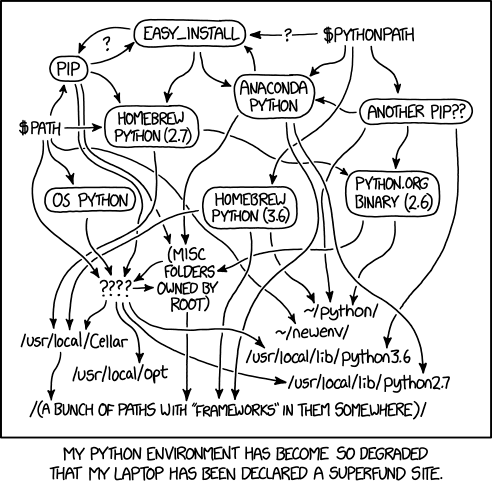
\includegraphics[width=6.83in]{figures/advanced/python-environment} \caption{XKCD on Python Environments (from https://xkcd.com/1987/)}\label{fig:xkcd}
\end{figure}

\hypertarget{how-can-i-access-data-across-languages}{%
\subsection{How can I access data across languages?}\label{how-can-i-access-data-across-languages}}

The most common way to use reticulate is to do some calculations in Python and then use the results in R
or vice versa.
To show how this works,
let's read our infant HIV data into a Pandas data frame:

\begin{Shaded}
\begin{Highlighting}[]
\ImportTok{import}\NormalTok{ pandas}
\NormalTok{data }\OperatorTok{=}\NormalTok{ pandas.read_csv(}\StringTok{'results/infant_hiv.csv'}\NormalTok{)}
\BuiltInTok{print}\NormalTok{(data.head())}
\end{Highlighting}
\end{Shaded}

\begin{verbatim}
  country  year  estimate  hi  lo
0     AFG  2009       NaN NaN NaN
1     AFG  2010       NaN NaN NaN
2     AFG  2011       NaN NaN NaN
3     AFG  2012       NaN NaN NaN
4     AFG  2013       NaN NaN NaN
\end{verbatim}

All of our Python variables are available in our R session as part of the \texttt{py} object,
so \texttt{py\$data} is our data frame inside a chunk of R code:

\begin{Shaded}
\begin{Highlighting}[]
\KeywordTok{library}\NormalTok{(reticulate)}
\KeywordTok{head}\NormalTok{(py}\OperatorTok{$}\NormalTok{data)}
\end{Highlighting}
\end{Shaded}

\begin{verbatim}
  country year estimate  hi  lo
1     AFG 2009      NaN NaN NaN
2     AFG 2010      NaN NaN NaN
3     AFG 2011      NaN NaN NaN
4     AFG 2012      NaN NaN NaN
5     AFG 2013      NaN NaN NaN
6     AFG 2014      NaN NaN NaN
\end{verbatim}

reticulate handles type conversions automatically,
though there are a few tricky cases:
for example,
the number \texttt{9} is a float in R,
so if you want an integer in Python,
you have to add the trailing \texttt{L} (for ``long'') and write it \texttt{9L}.

On the other hand,
reticulate translates between 0-based and 1-based indexing.
Suppose we create a character vector in R:

\begin{Shaded}
\begin{Highlighting}[]
\NormalTok{elements =}\StringTok{ }\KeywordTok{c}\NormalTok{(}\StringTok{'hydrogen'}\NormalTok{, }\StringTok{'helium'}\NormalTok{, }\StringTok{'lithium'}\NormalTok{, }\StringTok{'beryllium'}\NormalTok{)}
\end{Highlighting}
\end{Shaded}

Hydrogen is in position 1 in R:

\begin{Shaded}
\begin{Highlighting}[]
\NormalTok{elements[}\DecValTok{1}\NormalTok{]}
\end{Highlighting}
\end{Shaded}

\begin{verbatim}
[1] "hydrogen"
\end{verbatim}

but position 0 in Python:

\begin{Shaded}
\begin{Highlighting}[]
\BuiltInTok{print}\NormalTok{(r.elements[}\DecValTok{0}\NormalTok{])}
\end{Highlighting}
\end{Shaded}

\begin{verbatim}
hydrogen
\end{verbatim}

Note our use of the object \texttt{r} in our Python code:
just \texttt{py\$whatever} gives us access to Python objects in R,
\texttt{r.whatever} gives us access to R objects in Python.

\hypertarget{how-can-i-call-functions-across-languages}{%
\subsection{How can I call functions across languages?}\label{how-can-i-call-functions-across-languages}}

We don't have to run Python code,
store values in a variable,
and then access that variable from R:
we can call the Python directly (or vice versa).
For example,
we can use Python's random number generator in R as follows:

\begin{Shaded}
\begin{Highlighting}[]
\NormalTok{pyrand <-}\StringTok{ }\KeywordTok{import}\NormalTok{(}\StringTok{"random"}\NormalTok{)}
\NormalTok{pyrand}\OperatorTok{$}\KeywordTok{gauss}\NormalTok{(}\DecValTok{0}\NormalTok{, }\DecValTok{1}\NormalTok{)}
\end{Highlighting}
\end{Shaded}

\begin{verbatim}
[1] 2.163422
\end{verbatim}

(There's no reason to do this---R's random number generator is just as strong---but it illustrates the point.)

We can also source Python scripts.
For example,
suppose that \texttt{countries.py} contains this function:

\begin{Shaded}
\begin{Highlighting}[]
\CommentTok{#!/usr/bin/env python}

\ImportTok{import}\NormalTok{ pandas }\ImportTok{as}\NormalTok{ pd}

\KeywordTok{def}\NormalTok{ get_countries(filename):}
\NormalTok{    data }\OperatorTok{=}\NormalTok{ pd.read_csv(filename)}
    \ControlFlowTok{return}\NormalTok{ data.country.unique()}
\end{Highlighting}
\end{Shaded}

We can run that script using \texttt{source\_python}:

\begin{Shaded}
\begin{Highlighting}[]
\KeywordTok{source_python}\NormalTok{(}\StringTok{'countries.py'}\NormalTok{)}
\end{Highlighting}
\end{Shaded}

There is no output because all the script did was define a function.
By default,
that function and all other top-level variables defined in the script are now available in R:

\begin{Shaded}
\begin{Highlighting}[]
\KeywordTok{get_countries}\NormalTok{(}\StringTok{'results/infant_hiv.csv'}\NormalTok{)}
\end{Highlighting}
\end{Shaded}

\begin{verbatim}
  [1] "AFG" "AGO" "AIA" "ALB" "ARE" "ARG" "ARM" "ATG" "AUS" "AUT" "AZE"
 [12] "BDI" "BEL" "BEN" "BFA" "BGD" "BGR" "BHR" "BHS" "BIH" "BLR" "BLZ"
 [23] "BOL" "BRA" "BRB" "BRN" "BTN" "BWA" "CAF" "CAN" "CHE" "CHL" "CHN"
 [34] "CIV" "CMR" "COD" "COG" "COK" "COL" "COM" "CPV" "CRI" "CUB" "CYP"
 [45] "CZE" "DEU" "DJI" "DMA" "DNK" "DOM" "DZA" "ECU" "EGY" "ERI" "ESP"
 [56] "EST" "ETH" "FIN" "FJI" "FRA" "FSM" "GAB" "GBR" "GEO" "GHA" "GIN"
 [67] "GMB" "GNB" "GNQ" "GRC" "GRD" "GTM" "GUY" "HND" "HRV" "HTI" "HUN"
 [78] "IDN" "IND" "IRL" "IRN" "IRQ" "ISL" "ISR" "ITA" "JAM" "JOR" "JPN"
 [89] "KAZ" "KEN" "KGZ" "KHM" "KIR" "KNA" "KOR" "LAO" "LBN" "LBR" "LBY"
[100] "LCA" "LKA" "LSO" "LTU" "LUX" "LVA" "MAR" "MDA" "MDG" "MDV" "MEX"
[111] "MHL" "MKD" "MLI" "MLT" "MMR" "MNE" "MNG" "MOZ" "MRT" "MUS" "MWI"
[122] "MYS" "NAM" "NER" "NGA" "NIC" "NIU" "NLD" "NOR" "NPL" "NRU" "NZL"
[133] "OMN" "PAK" "PAN" "PER" "PHL" "PLW" "PNG" "POL" "PRK" "PRT" "PRY"
[144] "PSE" "ROU" "RUS" "RWA" "SAU" "SDN" "SEN" "SGP" "SLB" "SLE" "SLV"
[155] "SOM" "SRB" "SSD" "STP" "SUR" "SVK" "SVN" "SWE" "SWZ" "SYC" "SYR"
[166] "TCD" "TGO" "THA" "TJK" "TKM" "TLS" "TON" "TTO" "TUN" "TUR" "TUV"
[177] "TZA" "UGA" "UKR" "UNK" "URY" "USA" "UZB" "VCT" "VEN" "VNM" "VUT"
[188] "WSM" "YEM" "ZAF" "ZMB" "ZWE"
\end{verbatim}

There is one small pothole in this.
When the script is run,
the special Python variable \texttt{\_\_name\_\_} is set to \texttt{\textquotesingle{}\_\_main\_\_\textquotesingle{}"\textquotesingle{}},
i.e.,
the script thinks it is being called from the command line.
If it includes a conditional block to handle command-line arguments like this:

\begin{Shaded}
\begin{Highlighting}[]
\ControlFlowTok{if} \VariableTok{__name__} \OperatorTok{==} \StringTok{'__main__'}\NormalTok{:}
\NormalTok{    input_file, output_files }\OperatorTok{=}\NormalTok{ sys.argv[}\DecValTok{1}\NormalTok{], sys.argv[}\DecValTok{2}\NormalTok{:]}
\NormalTok{    main(input_file, output_files)}
\end{Highlighting}
\end{Shaded}

then that block will be executed,
but will fail because \texttt{sys.argv} won't include anything.

\hypertarget{how-does-object-oriented-programming-work-in-r}{%
\section{How does object-oriented programming work in R?}\label{how-does-object-oriented-programming-work-in-r}}

Programmers spend a great deal of their time trying to create order out of chaos,
and the rest of their time inventing new ways to create more chaos.
Object-oriented programming serves both needs well:
it allows good software designers to create marvels,
and less conscientious or less experienced ones to manufacture horrors.

R has not one, not two, but at least three different frameworks for object-oriented programming.
By far the most widely used is \protect\hyperlink{S3}{S3}
(because it was first introduced with Version 3 of S,
the language from which R is derived).
Unlike the approaches used in Python and similarly pedestrian languages,
S3 does not require users to define classes.
Instead,
they add \href{glossary.html\#attribute}{attributes} to data,
then write specialized versions of \href{glossary.html\#generic-function}{generic functions}
to process data identified by those attributes.
Since attributes can be used in other ways as well,
we will start by exploring them.

\hypertarget{what-are-attributes}{%
\subsection{What are attributes?}\label{what-are-attributes}}

Let's begin by creating a matrix containing the first few hundreds:

\begin{Shaded}
\begin{Highlighting}[]
\NormalTok{values <-}\StringTok{ }\DecValTok{100} \OperatorTok{*}\StringTok{ }\DecValTok{1}\OperatorTok{:}\DecValTok{9} \CommentTok{# creates c(100, 200, ..., 900)}
\NormalTok{m <-}\StringTok{ }\KeywordTok{matrix}\NormalTok{(values, }\DataTypeTok{nrow =} \DecValTok{3}\NormalTok{, }\DataTypeTok{ncol =} \DecValTok{3}\NormalTok{)}
\NormalTok{m}
\end{Highlighting}
\end{Shaded}

\begin{verbatim}
     [,1] [,2] [,3]
[1,]  100  400  700
[2,]  200  500  800
[3,]  300  600  900
\end{verbatim}

Behind the scenes,
R continues to store our nine values as a vector.
However,
it adds an attribute called \texttt{class} to the vector to identify it as a matrix:

\begin{Shaded}
\begin{Highlighting}[]
\KeywordTok{class}\NormalTok{(m)}
\end{Highlighting}
\end{Shaded}

\begin{verbatim}
[1] "matrix"
\end{verbatim}

and another attribute called \texttt{dim} to store its dimensions as a 2-element vector:

\begin{Shaded}
\begin{Highlighting}[]
\KeywordTok{dim}\NormalTok{(m)}
\end{Highlighting}
\end{Shaded}

\begin{verbatim}
[1] 3 3
\end{verbatim}

An object's attributes are simply a set of name-value pairs.
We can find out what attributes are present using \texttt{attributes} and show or set individual attributes using \texttt{attr}:

\begin{Shaded}
\begin{Highlighting}[]
\KeywordTok{attr}\NormalTok{(m, }\StringTok{"prospects"}\NormalTok{) <-}\StringTok{ "dismal"}
\KeywordTok{attributes}\NormalTok{(m)}
\end{Highlighting}
\end{Shaded}

\begin{verbatim}
$dim
[1] 3 3

$prospects
[1] "dismal"
\end{verbatim}

What are the type and attributes of a tibble?

\begin{Shaded}
\begin{Highlighting}[]
\NormalTok{t <-}\StringTok{ }\KeywordTok{tribble}\NormalTok{(}
  \OperatorTok{~}\NormalTok{a, }\OperatorTok{~}\NormalTok{b,}
  \DecValTok{1}\NormalTok{, }\DecValTok{2}\NormalTok{,}
  \DecValTok{3}\NormalTok{, }\DecValTok{4}\NormalTok{)}
\KeywordTok{typeof}\NormalTok{(t)}
\end{Highlighting}
\end{Shaded}

\begin{verbatim}
[1] "list"
\end{verbatim}

\begin{Shaded}
\begin{Highlighting}[]
\KeywordTok{attributes}\NormalTok{(t)}
\end{Highlighting}
\end{Shaded}

\begin{verbatim}
$names
[1] "a" "b"

$row.names
[1] 1 2

$class
[1] "tbl_df"     "tbl"        "data.frame"
\end{verbatim}

This tells us that a tibble is stored as a list (the first line of output),
and that it has an attribute called \texttt{names} that stores the names of its columns,
another called \texttt{row.names} that stores the names of its rows (a feature we should ignore),
and three classes.
These classes tell R what functions to search for when we are (for example)
asking for the length of a tibble (which is the number of rows it contains):

\begin{Shaded}
\begin{Highlighting}[]
\KeywordTok{length}\NormalTok{(t)}
\end{Highlighting}
\end{Shaded}

\begin{verbatim}
[1] 2
\end{verbatim}

\hypertarget{how-are-classes-represented}{%
\subsection{How are classes represented?}\label{how-are-classes-represented}}

To show how classes and generic functions work together,
let's customize the way that 2D coordinates are converted to strings.
First,
we create two coordinate vectors:

\begin{Shaded}
\begin{Highlighting}[]
\NormalTok{first <-}\StringTok{ }\KeywordTok{c}\NormalTok{(}\FloatTok{0.5}\NormalTok{, }\FloatTok{0.7}\NormalTok{)}
\KeywordTok{class}\NormalTok{(first) <-}\StringTok{ "two_d"}
\KeywordTok{print}\NormalTok{(first)}
\end{Highlighting}
\end{Shaded}

\begin{verbatim}
[1] 0.5 0.7
attr(,"class")
[1] "two_d"
\end{verbatim}

\begin{Shaded}
\begin{Highlighting}[]
\NormalTok{second <-}\StringTok{ }\KeywordTok{c}\NormalTok{(}\FloatTok{1.3}\NormalTok{, }\FloatTok{3.1}\NormalTok{)}
\KeywordTok{class}\NormalTok{(second) <-}\StringTok{ "two_d"}
\KeywordTok{print}\NormalTok{(second)}
\end{Highlighting}
\end{Shaded}

\begin{verbatim}
[1] 1.3 3.1
attr(,"class")
[1] "two_d"
\end{verbatim}

Separately, we define the behavior of \texttt{toString} for such objects:

\begin{Shaded}
\begin{Highlighting}[]
\NormalTok{toString.two_d <-}\StringTok{ }\ControlFlowTok{function}\NormalTok{(obj)\{}
  \KeywordTok{paste0}\NormalTok{(}\StringTok{"<"}\NormalTok{, obj[}\DecValTok{1}\NormalTok{], }\StringTok{", "}\NormalTok{, obj[}\DecValTok{2}\NormalTok{], }\StringTok{">"}\NormalTok{)}
\NormalTok{\}}
\KeywordTok{toString}\NormalTok{(first)}
\end{Highlighting}
\end{Shaded}

\begin{verbatim}
[1] "<0.5, 0.7>"
\end{verbatim}

\begin{Shaded}
\begin{Highlighting}[]
\KeywordTok{toString}\NormalTok{(second)}
\end{Highlighting}
\end{Shaded}

\begin{verbatim}
[1] "<1.3, 3.1>"
\end{verbatim}

S3's protocol is simple:
given a function F and an object of class C,
S3 looks for a function named F.C.
If it doesn't find one,
it looks at the object's next class (assuming it has more than one);
once its user-assigned classes are exhausted,
it uses whatever function the system has defined for its base type (in this case, character vector).
We can trace this process by importing the sloop package and calling \texttt{s3\_dispatch}:

\begin{Shaded}
\begin{Highlighting}[]
\KeywordTok{library}\NormalTok{(sloop)}
\KeywordTok{s3_dispatch}\NormalTok{(}\KeywordTok{toString}\NormalTok{(first))}
\end{Highlighting}
\end{Shaded}

\begin{verbatim}
=> toString.two_d
 * toString.default
\end{verbatim}

Compare this with calling \texttt{toString} on a plain old character vector:

\begin{Shaded}
\begin{Highlighting}[]
\KeywordTok{s3_dispatch}\NormalTok{(}\KeywordTok{toString}\NormalTok{(}\KeywordTok{c}\NormalTok{(}\FloatTok{7.1}\NormalTok{, }\FloatTok{7.2}\NormalTok{)))}
\end{Highlighting}
\end{Shaded}

\begin{verbatim}
   toString.double
   toString.numeric
=> toString.default
\end{verbatim}

The specialized functions associated with a generic function like \texttt{toString} are called \href{glossary.html\#method}{methods}.
Unlike languages that require methods to be defined all together as part of a class,
S3 allows us to add methods when and as we see fit.
But that doesn't mean we should:
minds confined to three dimensions of space and one of time are simply not capable of comprehending
complex class hierarchies.
Instead,
we should always write three functions that work together for a class like \texttt{two\_d}:

\begin{itemize}
\tightlist
\item
  A \href{glossary.html\#constructor}{constructor} called \texttt{new\_two\_d}
  that creates objects of our class.
\item
  An optional \href{glossary.html\#validator}{validator} called \texttt{validate\_two\_d}
  that checks the consistency and correctness of an object's values.
\item
  An optional \href{glossary.html\#helper}{helper}, simply called \texttt{two\_d},
  that most users will call to create and validate objects.
\end{itemize}

The constructor's first argument should always be the base object (in our case, the two-element vector).
It should also have one argument for each attribute the object is to have, if any.
Unlike matrices, our 2D points don't have any extra arguments, so our constructor needs no extra arguments.
Crucially,
the constructor checks the type of its arguments to ensure that the object has at least some chance of being valid.

\begin{Shaded}
\begin{Highlighting}[]
\NormalTok{new_two_d <-}\StringTok{ }\ControlFlowTok{function}\NormalTok{(coordinates)\{}
  \KeywordTok{stopifnot}\NormalTok{(}\KeywordTok{is.numeric}\NormalTok{(coordinates))}
  \KeywordTok{class}\NormalTok{(coordinates) <-}\StringTok{ "two_d"}
\NormalTok{  coordinates}
\NormalTok{\}}

\NormalTok{example <-}\StringTok{ }\KeywordTok{new_two_d}\NormalTok{(}\KeywordTok{c}\NormalTok{(}\FloatTok{4.4}\NormalTok{, }\FloatTok{-2.2}\NormalTok{))}
\KeywordTok{toString}\NormalTok{(example)}
\end{Highlighting}
\end{Shaded}

\begin{verbatim}
[1] "<4.4, -2.2>"
\end{verbatim}

Validators are only needed when checks on data correctness and consistency are expensive.
For example,
if we were to define a class to represent sorted vectors,
checking that each element is no less than its predecessor could take a long time for very long vectors.
To illustrate this,
we will check that we have exactly two coordinates;
in real code,
we would probably include this (inexpensive) check in the constructor.

\begin{Shaded}
\begin{Highlighting}[]
\NormalTok{validate_two_d <-}\StringTok{ }\ControlFlowTok{function}\NormalTok{(coordinates) \{}
  \KeywordTok{stopifnot}\NormalTok{(}\KeywordTok{length}\NormalTok{(coordinates) }\OperatorTok{==}\StringTok{ }\DecValTok{2}\NormalTok{)}
  \KeywordTok{stopifnot}\NormalTok{(}\KeywordTok{class}\NormalTok{(coordinates) }\OperatorTok{==}\StringTok{ "two_d"}\NormalTok{)}
\NormalTok{\}}

\KeywordTok{validate_two_d}\NormalTok{(example)    }\CommentTok{# should succeed silently}
\KeywordTok{validate_two_d}\NormalTok{(}\KeywordTok{c}\NormalTok{(}\DecValTok{1}\NormalTok{, }\DecValTok{3}\NormalTok{))    }\CommentTok{# should fail}
\end{Highlighting}
\end{Shaded}

\begin{verbatim}
Error in validate_two_d(c(1, 3)): class(coordinates) == "two_d" is not TRUE
\end{verbatim}

\begin{Shaded}
\begin{Highlighting}[]
\KeywordTok{validate_two_d}\NormalTok{(}\KeywordTok{c}\NormalTok{(}\DecValTok{2}\NormalTok{, }\DecValTok{2}\NormalTok{, }\DecValTok{2}\NormalTok{)) }\CommentTok{# should also fail}
\end{Highlighting}
\end{Shaded}

\begin{verbatim}
Error in validate_two_d(c(2, 2, 2)): length(coordinates) == 2 is not TRUE
\end{verbatim}

The third and final function in our trio provides a user-friendly way to construct objects of our new class.
It should call the constructor and the validator (if one exists),
but should also provide a richer set of defaults,
better error messages,
and so on.
To illustrate this,
we shall allow the user to provide either one argument (which must be a two-element vector)
or two (which must each be numeric):

\begin{Shaded}
\begin{Highlighting}[]
\NormalTok{two_d <-}\StringTok{ }\ControlFlowTok{function}\NormalTok{(...)\{}
\NormalTok{  args <-}\StringTok{ }\KeywordTok{list}\NormalTok{(...)}
  \ControlFlowTok{if}\NormalTok{ (}\KeywordTok{length}\NormalTok{(args) }\OperatorTok{==}\StringTok{ }\DecValTok{1}\NormalTok{) \{}
\NormalTok{    args <-}\StringTok{ }\NormalTok{args[[}\DecValTok{1}\NormalTok{]]    }\CommentTok{# extract original value}
\NormalTok{  \}}
  \ControlFlowTok{else} \ControlFlowTok{if}\NormalTok{ (}\KeywordTok{length}\NormalTok{(args) }\OperatorTok{==}\StringTok{ }\DecValTok{2}\NormalTok{) \{}
\NormalTok{    args <-}\StringTok{ }\KeywordTok{unlist}\NormalTok{(args) }\CommentTok{# convert list to vector}
\NormalTok{  \}}
\NormalTok{  result <-}\StringTok{ }\KeywordTok{new_two_d}\NormalTok{(args)}
  \KeywordTok{validate_two_d}\NormalTok{(result)}
\NormalTok{  result}
\NormalTok{\}}

\NormalTok{here <-}\StringTok{ }\KeywordTok{two_d}\NormalTok{(}\FloatTok{10.1}\NormalTok{, }\FloatTok{11.2}\NormalTok{)}
\KeywordTok{toString}\NormalTok{(here)}
\end{Highlighting}
\end{Shaded}

\begin{verbatim}
[1] "<10.1, 11.2>"
\end{verbatim}

\begin{Shaded}
\begin{Highlighting}[]
\NormalTok{there <-}\StringTok{ }\KeywordTok{two_d}\NormalTok{(}\KeywordTok{c}\NormalTok{(}\FloatTok{15.6}\NormalTok{, }\FloatTok{16.7}\NormalTok{))}
\KeywordTok{toString}\NormalTok{(there)}
\end{Highlighting}
\end{Shaded}

\begin{verbatim}
[1] "<15.6, 16.7>"
\end{verbatim}

\hypertarget{how-does-inheritance-work}{%
\subsection{How does inheritance work?}\label{how-does-inheritance-work}}

We said above that an object can have more than one class,
and that S3 searches the classes in order when it wants to find a method to call.
Methods can also trigger invocation of other methods explicitly in order to supplement,
rather than replace,
the behavior of other classes.
To show how this works,
we shall look at that classic of object-oriented design: shapes.
(The safe kind,
of course,
not those whose non-Euclidean angles have placed such intolerable stress on the minds of so many of our colleagues over the years.)
We start by defining a \texttt{polygon} class:

\begin{Shaded}
\begin{Highlighting}[]
\NormalTok{new_polygon <-}\StringTok{ }\ControlFlowTok{function}\NormalTok{(coords, name) \{}
\NormalTok{  points <-}\StringTok{ }\KeywordTok{map}\NormalTok{(coords, two_d)}
  \KeywordTok{class}\NormalTok{(points) <-}\StringTok{ "polygon"}
  \KeywordTok{attr}\NormalTok{(points, }\StringTok{"name"}\NormalTok{) <-}\StringTok{ }\NormalTok{name}
\NormalTok{  points}
\NormalTok{\}}

\NormalTok{toString.polygon <-}\StringTok{ }\ControlFlowTok{function}\NormalTok{(poly) \{}
  \KeywordTok{paste0}\NormalTok{(}\KeywordTok{attr}\NormalTok{(poly, }\StringTok{"name"}\NormalTok{), }\StringTok{": "}\NormalTok{, }\KeywordTok{paste0}\NormalTok{(}\KeywordTok{map}\NormalTok{(poly, toString), }\DataTypeTok{collapse =} \StringTok{", "}\NormalTok{))}
\NormalTok{\}}

\NormalTok{right <-}\StringTok{ }\KeywordTok{new_polygon}\NormalTok{(}\KeywordTok{list}\NormalTok{(}\KeywordTok{c}\NormalTok{(}\DecValTok{0}\NormalTok{, }\DecValTok{0}\NormalTok{), }\KeywordTok{c}\NormalTok{(}\DecValTok{1}\NormalTok{, }\DecValTok{0}\NormalTok{), }\KeywordTok{c}\NormalTok{(}\DecValTok{0}\NormalTok{, }\DecValTok{1}\NormalTok{)), }\StringTok{"triangle"}\NormalTok{)}
\KeywordTok{toString}\NormalTok{(right)}
\end{Highlighting}
\end{Shaded}

\begin{verbatim}
[1] "triangle: <0, 0>, <1, 0>, <0, 1>"
\end{verbatim}

Now we will add colored shapes:

\begin{Shaded}
\begin{Highlighting}[]
\NormalTok{new_colored_polygon <-}\StringTok{ }\ControlFlowTok{function}\NormalTok{(coords, name, color) \{}
\NormalTok{  object <-}\StringTok{ }\KeywordTok{new_polygon}\NormalTok{(coords, name)}
  \KeywordTok{attr}\NormalTok{(object, }\StringTok{"color"}\NormalTok{) <-}\StringTok{ }\NormalTok{color}
  \KeywordTok{class}\NormalTok{(object) <-}\StringTok{ }\KeywordTok{c}\NormalTok{(}\StringTok{"colored_polygon"}\NormalTok{, }\KeywordTok{class}\NormalTok{(object))}
\NormalTok{  object}
\NormalTok{\}}

\NormalTok{pinkish <-}\StringTok{ }\KeywordTok{new_colored_polygon}\NormalTok{(}\KeywordTok{list}\NormalTok{(}\KeywordTok{c}\NormalTok{(}\DecValTok{0}\NormalTok{, }\DecValTok{0}\NormalTok{), }\KeywordTok{c}\NormalTok{(}\DecValTok{1}\NormalTok{, }\DecValTok{0}\NormalTok{), }\KeywordTok{c}\NormalTok{(}\DecValTok{1}\NormalTok{, }\DecValTok{1}\NormalTok{)), }\StringTok{"triangle"}\NormalTok{, }\StringTok{"roseate"}\NormalTok{)}
\KeywordTok{class}\NormalTok{(pinkish)}
\end{Highlighting}
\end{Shaded}

\begin{verbatim}
[1] "colored_polygon" "polygon"        
\end{verbatim}

\begin{Shaded}
\begin{Highlighting}[]
\KeywordTok{toString}\NormalTok{(pinkish)}
\end{Highlighting}
\end{Shaded}

\begin{verbatim}
[1] "triangle: <0, 0>, <1, 0>, <1, 1>"
\end{verbatim}

So far so good:
since we have not defined a method to handle colored polygons specifically,
we get the behavior for a regular polygon.
Let's add another method that supplements the behavior of the existing method:

\begin{Shaded}
\begin{Highlighting}[]
\NormalTok{toString.colored_polygon <-}\StringTok{ }\ControlFlowTok{function}\NormalTok{(poly) \{}
  \KeywordTok{paste0}\NormalTok{(}\KeywordTok{toString.polygon}\NormalTok{(poly), }\StringTok{"+ color = "}\NormalTok{, }\KeywordTok{attr}\NormalTok{(poly, }\StringTok{"color"}\NormalTok{))}
\NormalTok{\}}

\KeywordTok{toString}\NormalTok{(pinkish)}
\end{Highlighting}
\end{Shaded}

\begin{verbatim}
[1] "triangle: <0, 0>, <1, 0>, <1, 1>+ color = roseate"
\end{verbatim}

In practice,
we will almost always place all of the methods associated with a class in the same file as its constructor, validator, and helper.
The time has finally come for us to explore projects and packages.

\hypertarget{how-can-i-write-web-applications-in-r}{%
\section{How can I write web applications in R?}\label{how-can-i-write-web-applications-in-r}}

R has this awesome gnarly web programming framework called Shiny.
It uses \sout{sympathetic magic} \sout{quantum entanglement} reactive variables
to update the application's interface when data changes.
You should, like, totally check it out.

\hypertarget{how-can-i-work-with-relational-databases-in-r}{%
\section{How can I work with relational databases in R?}\label{how-can-i-work-with-relational-databases-in-r}}

Data frames and database tables go together as naturally as chocolate and the tears of our fallen foes.
As in Python and other languages,
there is a standard interface for connecting to and querying relational databases;
each database is then supported by a package that implements that interface.
This doesn't completely hide the differences between databases---we must still worry about
the quirks of various SQL dialects---but it does keep the R side of things simple.

This tutorial uses the SQLite database and the RSQLite interface package.
The former is included with the latter,
so \texttt{install.packages("RSQLite")} will give you everything you need.
We assume that you already speak enough SQL to get yourself into trouble;
if you do not, \href{https://swcarpentry.github.io/sql-novice-survey/}{this tutorial} is a good place to start.

\hypertarget{how-can-i-get-data-from-a-database}{%
\subsection{How can I get data from a database?}\label{how-can-i-get-data-from-a-database}}

Suppose we have a small database in \texttt{data/example.db}
containing survey data salvaged from a series of doomed expeditions to the Antarctic in the 1920s and 1930s.
The database contains four tables:

\textbf{Person}: people who took readings.

\begin{longtable}[]{@{}lll@{}}
\toprule
person\_id & personal & family\tabularnewline
\midrule
\endhead
dyer & William & Dyer\tabularnewline
pb & Frank & Pabodie\tabularnewline
lake & Anderson & Lake\tabularnewline
roe & Valentina & Roerich\tabularnewline
danforth & Frank & Danforth\tabularnewline
\bottomrule
\end{longtable}

\textbf{Site}: locations where readings were taken.

\begin{longtable}[]{@{}lll@{}}
\toprule
site\_id & lat & long\tabularnewline
\midrule
\endhead
DR-1 & -49.85 & -128.57\tabularnewline
DR-3 & -47.15 & -126.72\tabularnewline
MSK-4 & -48.87 & -123.4\tabularnewline
\bottomrule
\end{longtable}

\textbf{Visited}: when readings were taken at specific sites.

\begin{longtable}[]{@{}lll@{}}
\toprule
visit\_id & site\_id & dated\tabularnewline
\midrule
\endhead
619 & DR-1 & 1927-02-08\tabularnewline
622 & DR-1 & 1927-02-10\tabularnewline
734 & DR-3 & 1930-01-07\tabularnewline
735 & DR-3 & 1930-01-12\tabularnewline
751 & DR-3 & 1930-02-26\tabularnewline
752 & DR-3 & -null-\tabularnewline
837 & MSK-4 & 1932-01-14\tabularnewline
844 & DR-1 & 1932-03-22\tabularnewline
\bottomrule
\end{longtable}

\textbf{Measurements}: the actual readings.

\begin{longtable}[]{@{}llll@{}}
\toprule
visit\_id & visitor & quantity & reading\tabularnewline
\midrule
\endhead
619 & dyer & rad & 9.82\tabularnewline
619 & dyer & sal & 0.13\tabularnewline
622 & dyer & rad & 7.8\tabularnewline
622 & dyer & sal & 0.09\tabularnewline
734 & pb & rad & 8.41\tabularnewline
734 & lake & sal & 0.05\tabularnewline
734 & pb & temp & -21.5\tabularnewline
735 & pb & rad & 7.22\tabularnewline
735 & -null- & sal & 0.06\tabularnewline
735 & -null- & temp & -26.0\tabularnewline
751 & pb & rad & 4.35\tabularnewline
751 & pb & temp & -18.5\tabularnewline
751 & lake & sal & 0.1\tabularnewline
752 & lake & rad & 2.19\tabularnewline
752 & lake & sal & 0.09\tabularnewline
752 & lake & temp & -16.0\tabularnewline
752 & roe & sal & 41.6\tabularnewline
837 & lake & rad & 1.46\tabularnewline
837 & lake & sal & 0.21\tabularnewline
837 & roe & sal & 22.5\tabularnewline
844 & roe & rad & 11.25\tabularnewline
\bottomrule
\end{longtable}

Let's get the data about the people into a data frame:

\begin{Shaded}
\begin{Highlighting}[]
\KeywordTok{library}\NormalTok{(DBI)}
\NormalTok{db <-}\StringTok{ }\KeywordTok{dbConnect}\NormalTok{(RSQLite}\OperatorTok{::}\KeywordTok{SQLite}\NormalTok{(), here}\OperatorTok{::}\KeywordTok{here}\NormalTok{(}\StringTok{"data"}\NormalTok{, }\StringTok{"example.db"}\NormalTok{))}
\KeywordTok{dbGetQuery}\NormalTok{(db, }\StringTok{"select * from Person;"}\NormalTok{)}
\end{Highlighting}
\end{Shaded}

\begin{verbatim}
  person_id personal_name family_name
1      dyer       William        Dyer
2        pb         Frank     Pabodie
3      lake      Anderson        Lake
4       roe     Valentina     Roerich
5  danforth         Frank    Danforth
\end{verbatim}

That seems simple enough:
the database connection is the first argument to \texttt{dbGetQuery},
the query itself is the second,
and the result is a tibble whose column names correspond to the names of the fields in the database table.
What if we want to parameterize our query?
Inside the text of the query,
we use \texttt{:name} as a placeholder for a query parameter,
then pass a list of name-value pairs to specify what we actually want:

\begin{Shaded}
\begin{Highlighting}[]
\KeywordTok{dbGetQuery}\NormalTok{(db,}
           \StringTok{"select * from Measurements where quantity = :desired"}\NormalTok{,}
           \DataTypeTok{params =} \KeywordTok{list}\NormalTok{(}\DataTypeTok{desired =} \StringTok{"rad"}\NormalTok{))}
\end{Highlighting}
\end{Shaded}

\begin{verbatim}
  visit_id person_id quantity reading
1      619      dyer      rad    9.82
2      622      dyer      rad    7.80
3      734        pb      rad    8.41
4      735        pb      rad    7.22
5      751        pb      rad    4.35
6      752      lake      rad    2.19
7      837      lake      rad    1.46
8      844       roe      rad   11.25
\end{verbatim}

Do \emph{not} use \texttt{glue} or some other kind of string interpolation to construct database queries,
as this can leave you open to \href{https://en.wikipedia.org/wiki/SQL_injection}{SQL injection attacks}
and other forms of digital damnation.

If you expect a large set of results,
it's best to page through them:

\begin{Shaded}
\begin{Highlighting}[]
\NormalTok{results <-}\StringTok{ }\KeywordTok{dbSendQuery}\NormalTok{(db, }\StringTok{"select * from Measurements limit 15;"}\NormalTok{)}
\ControlFlowTok{while}\NormalTok{ (}\OperatorTok{!}\KeywordTok{dbHasCompleted}\NormalTok{(results)) \{}
\NormalTok{  chunk <-}\StringTok{ }\KeywordTok{dbFetch}\NormalTok{(results, }\DataTypeTok{n =} \DecValTok{3}\NormalTok{) }\CommentTok{# artificially low for tutorial purposes}
  \KeywordTok{print}\NormalTok{(chunk)}
\NormalTok{\}}
\end{Highlighting}
\end{Shaded}

\begin{verbatim}
  visit_id person_id quantity reading
1      619      dyer      rad    9.82
2      619      dyer      sal    0.13
3      622      dyer      rad    7.80
  visit_id person_id quantity reading
1      622      dyer      sal    0.09
2      734        pb      rad    8.41
3      734      lake      sal    0.05
  visit_id person_id quantity reading
1      734        pb     temp  -21.50
2      735        pb      rad    7.22
3      735      <NA>      sal    0.06
  visit_id person_id quantity reading
1      735      <NA>     temp  -26.00
2      751        pb      rad    4.35
3      751        pb     temp  -18.50
\end{verbatim}

\begin{verbatim}
Warning in result_fetch(res@ptr, n = n): Column `reading`: mixed type,
first seen values of type real, coercing other values of type string
\end{verbatim}

\begin{verbatim}
  visit_id person_id quantity reading
1      751      lake      sal    0.00
2      752      lake      rad    2.19
3      752      lake      sal    0.09
\end{verbatim}

\begin{Shaded}
\begin{Highlighting}[]
\KeywordTok{dbClearResult}\NormalTok{(results)}
\end{Highlighting}
\end{Shaded}

\hypertarget{how-can-i-populate-databases-with-r}{%
\subsection{How can I populate databases with R?}\label{how-can-i-populate-databases-with-r}}

Data scientists spend most of their time reading data, but someone has to create it.
RSQLite makes it easy to map a data frame directly to a database table;
to show how it works,
we will create an in-memory database:

\begin{Shaded}
\begin{Highlighting}[]
\NormalTok{colors <-}\StringTok{ }\KeywordTok{tribble}\NormalTok{(}
  \OperatorTok{~}\NormalTok{name, }\OperatorTok{~}\NormalTok{red, }\OperatorTok{~}\NormalTok{green, }\OperatorTok{~}\NormalTok{blue,}
  \StringTok{'black'}\NormalTok{, }\DecValTok{0}\NormalTok{, }\DecValTok{0}\NormalTok{, }\DecValTok{0}\NormalTok{,}
  \StringTok{'yellow'}\NormalTok{, }\DecValTok{255}\NormalTok{, }\DecValTok{255}\NormalTok{, }\DecValTok{0}\NormalTok{,}
  \StringTok{'aqua'}\NormalTok{, }\DecValTok{0}\NormalTok{, }\DecValTok{255}\NormalTok{, }\DecValTok{255}\NormalTok{,}
  \StringTok{'fuchsia'}\NormalTok{, }\DecValTok{255}\NormalTok{, }\DecValTok{0}\NormalTok{, }\DecValTok{0}
\NormalTok{)}
\NormalTok{db <-}\StringTok{ }\KeywordTok{dbConnect}\NormalTok{(RSQLite}\OperatorTok{::}\KeywordTok{SQLite}\NormalTok{(), }\StringTok{':memory:'}\NormalTok{)}
\KeywordTok{dbWriteTable}\NormalTok{(db, }\StringTok{"colors"}\NormalTok{, colors)}
\end{Highlighting}
\end{Shaded}

Let's see what the combination of R and SQLite has done with our data and the types thereof:

\begin{Shaded}
\begin{Highlighting}[]
\KeywordTok{dbGetQuery}\NormalTok{(db, }\StringTok{"select * from colors;"}\NormalTok{)}
\end{Highlighting}
\end{Shaded}

\begin{verbatim}
     name red green blue
1   black   0     0    0
2  yellow 255   255    0
3    aqua   0   255  255
4 fuchsia 255     0    0
\end{verbatim}

Good: the types have been guessed correctly.

But what about dates?

\begin{Shaded}
\begin{Highlighting}[]
\NormalTok{appointments <-}\StringTok{ }\KeywordTok{tribble}\NormalTok{(}
  \OperatorTok{~}\NormalTok{who, }\OperatorTok{~}\NormalTok{when,}
  \StringTok{'Dyer'}\NormalTok{, }\StringTok{'1927-03-01'}\NormalTok{,}
  \StringTok{'Peabody'}\NormalTok{, }\StringTok{'1927-05-05'}
\NormalTok{) }\OperatorTok\StringTok{ }\KeywordTok{mutate}\NormalTok{(}\DataTypeTok{when =}\NormalTok{ lubridate}\OperatorTok{::}\KeywordTok{as_date}\NormalTok{(when))}
\KeywordTok{dbWriteTable}\NormalTok{(db, }\StringTok{"appointments"}\NormalTok{, appointments)}
\KeywordTok{dbGetQuery}\NormalTok{(db, }\StringTok{"select * from appointments;"}\NormalTok{)}
\end{Highlighting}
\end{Shaded}

\begin{verbatim}
      who   when
1    Dyer -15647
2 Peabody -15582
\end{verbatim}

What fresh hell is this?
After considerable trial and error,
we discover that our dates have been returned to us as
the number of days since January 1, 1970:

\begin{Shaded}
\begin{Highlighting}[]
\KeywordTok{dbExecute}\NormalTok{(db,}
           \StringTok{"insert into appointments values('Testing', :the_date);"}\NormalTok{,}
           \DataTypeTok{params =} \KeywordTok{list}\NormalTok{(}\DataTypeTok{the_date =}\NormalTok{ lubridate}\OperatorTok{::}\KeywordTok{as_date}\NormalTok{(}\StringTok{'1971-01-01'}\NormalTok{)))}
\end{Highlighting}
\end{Shaded}

\begin{verbatim}
[1] 1
\end{verbatim}

\begin{Shaded}
\begin{Highlighting}[]
\KeywordTok{dbGetQuery}\NormalTok{(db, }\StringTok{"select * from appointments where who = 'Testing';"}\NormalTok{)}
\end{Highlighting}
\end{Shaded}

\begin{verbatim}
      who when
1 Testing  365
\end{verbatim}

There is no point screaming:
those who might pity you cannot hear,
and those who can hear will definitely not pity you.

\hypertarget{key-points-7}{%
\section{Key Points}\label{key-points-7}}

\begin{itemize}
\tightlist
\item
  The \texttt{reticulate} library allows R programs to access data in Python programs and vice versa.
\item
  Use \texttt{py.whatever} to access a top-level Python variable from R.
\item
  Use \texttt{r.whatever} to access a top-level R definition from Python.
\item
  R is always indexed from 1 (even in Python) and Python is always indexed from 0 (even in R).
\item
  Numbers in R are floating point by default, so use a trailing `L' to force a value to be an integer.
\item
  A Python script run from an R session believes it is the main script, i.e., \texttt{\_\_name\_\_} is \texttt{\textquotesingle{}\_\_main\_\_\textquotesingle{}} inside the Python script.
\item
  S3 is the most commonly used object-oriented programming system in R.
\item
  Every object can store metadata about itself in attributes, which are set and queried with \texttt{attr}.
\item
  The \texttt{dim} attribute stores the dimensions of a matrix (which is physically stored as a vector).
\item
  The \texttt{class} attribute of an object defines its class or classes (it may have several character entries).
\item
  When \texttt{F(X,\ ...)} is called, and \texttt{X} has class \texttt{C}, R looks for a function called \texttt{F.C} (the \texttt{.} is just a naming convention).
\item
  If an object has multiple classes in its \texttt{class} attribute, R looks for a corresponding method for each in turn.
\item
  Every user defined class \texttt{C} should have functions \texttt{new\_C} (to create it), \texttt{validate\_C} (to validate its integrity), and \texttt{C} (to create and validate).
\item
  Use the \texttt{DBI} package to work with relational databases.
\item
  Use \texttt{DBI::dbConnect(...)} with database-specific parameters to connect to a specific database.
\item
  Use \texttt{dbGetQuery(connection,\ "query")} to send an SQL query string to a database and get a data frame of results.
\item
  Parameterize queries using \texttt{:name} as a placeholder in the query and \texttt{params~=~list(name~=~value)} as a third parameter to \texttt{dbGetQuery} to specify actual values.
\item
  Use \texttt{dbFetch} in a \texttt{while} loop to page results.
\item
  Use \texttt{dbWriteTable} to write an entire data frame to a table, and \texttt{dbExecute} to execute a single insertion statement.
\item
  Dates\ldots{} why did it have to be dates?
\end{itemize}

\cleardoublepage

\hypertarget{appendix-appendix}{%
\appendix}


\hypertarget{license}{%
\chapter{License}\label{license}}

\emph{This is a human-readable summary of (and not a substitute for) the license.
Please see \url{https://creativecommons.org/licenses/by/4.0/legalcode} for the full legal text.}

This work is licensed under the Creative Commons Attribution 4.0
International license (CC-BY-4.0).

\textbf{You are free to:}

\begin{itemize}
\item
  \textbf{Share}---copy and redistribute the material in any medium or
  format
\item
  \textbf{Remix}---remix, transform, and build upon the material for any
  purpose, even commercially.
\end{itemize}

The licensor cannot revoke these freedoms as long as you follow the
license terms.

\textbf{Under the following terms:}

\begin{itemize}
\item
  \textbf{Attribution}---You must give appropriate credit, provide a link
  to the license, and indicate if changes were made. You may do so in
  any reasonable manner, but not in any way that suggests the licensor
  endorses you or your use.
\item
  \textbf{No additional restrictions}---You may not apply legal terms or
  technological measures that legally restrict others from doing
  anything the license permits.
\end{itemize}

\textbf{Notices:}

You do not have to comply with the license for elements of the
material in the public domain or where your use is permitted by an
applicable exception or limitation.

No warranties are given. The license may not give you all of the
permissions necessary for your intended use. For example, other rights
such as publicity, privacy, or moral rights may limit how you use the
material.

\hypertarget{code-of-conduct}{%
\chapter{Code of Conduct}\label{code-of-conduct}}

In the interest of fostering an open and welcoming environment, we as
contributors and maintainers pledge to making participation in our project and
our community a harassment-free experience for everyone, regardless of age, body
size, disability, ethnicity, gender identity and expression, level of
experience, education, socio-economic status, nationality, personal appearance,
race, religion, or sexual identity and orientation.

\hypertarget{our-standards}{%
\section{Our Standards}\label{our-standards}}

Examples of behavior that contributes to creating a positive environment
include:

\begin{itemize}
\tightlist
\item
  using welcoming and inclusive language,
\item
  being respectful of differing viewpoints and experiences,
\item
  gracefully accepting constructive criticism,
\item
  focusing on what is best for the community, and
\item
  showing empathy towards other community members.
\end{itemize}

Examples of unacceptable behavior by participants include:

\begin{itemize}
\tightlist
\item
  the use of sexualized language or imagery and unwelcome sexual
  attention or advances,
\item
  trolling, insulting/derogatory comments, and personal or political
  attacks,
\item
  public or private harassment,
\item
  publishing others' private information, such as a physical or
  electronic address, without explicit permission, and
\item
  other conduct which could reasonably be considered inappropriate in
  a professional setting
\end{itemize}

\hypertarget{our-responsibilities}{%
\section{Our Responsibilities}\label{our-responsibilities}}

Project maintainers are responsible for clarifying the standards of acceptable
behavior and are expected to take appropriate and fair corrective action in
response to any instances of unacceptable behavior.

Project maintainers have the right and responsibility to remove, edit, or reject
comments, commits, code, wiki edits, issues, and other contributions that are
not aligned to this Code of Conduct, or to ban temporarily or permanently any
contributor for other behaviors that they deem inappropriate, threatening,
offensive, or harmful.

\hypertarget{scope}{%
\section{Scope}\label{scope}}

This Code of Conduct applies both within project spaces and in public spaces
when an individual is representing the project or its community. Examples of
representing a project or community include using an official project e-mail
address, posting via an official social media account, or acting as an appointed
representative at an online or offline event. Representation of a project may be
further defined and clarified by project maintainers.

\hypertarget{enforcement}{%
\section{Enforcement}\label{enforcement}}

Instances of abusive, harassing, or otherwise unacceptable behavior may be
reported by emailing the project team. All complaints will be reviewed and
investigated and will result in a response that is deemed necessary and
appropriate to the circumstances. The project team is obligated to maintain
confidentiality with regard to the reporter of an incident. Further details of
specific enforcement policies may be posted separately.

Project maintainers who do not follow or enforce the Code of Conduct in good
faith may face temporary or permanent repercussions as determined by other
members of the project's leadership.

\hypertarget{attribution}{%
\section{Attribution}\label{attribution}}

This Code of Conduct is adapted from the \href{https://www.contributor-covenant.org}{Contributor Covenant}
version 1.4.

\hypertarget{citation}{%
\chapter{Citation}\label{citation}}

Please cite this work as:

\begin{quote}
Greg Wilson: \emph{The Tidynomicon: A Brief Introduction to R for Python Programmers.}
\url{https://github.com/gvwilson/tidynomicon}, 2018.
\end{quote}

\hypertarget{contributing}{%
\chapter{Contributing}\label{contributing}}

Contributions of all kinds are welcome, from errata and minor improvements to
entirely new sections and chapters: please \href{mailto:\%7B\%7Bsite.email\%7D\%7D}{email us} or submit an
issue or pull request to \href{\%7B\%7Bsite.repo\%7D\%7D}{our GitHub repository}. Everyone whose
work is incorporated will be acknowledged; please note that all contributors are
required to abide by our Code of Conduct (\protect\hyperlink{REF}{s:conduct}).

The \href{https://jekyllrb.com/}{Jekyll} template used in this tutorial can support multiple
languages. All English content should go in the \texttt{\_en} directory. (Please note
that we use Simplified English rather than Traditional English, i.e., American
rather than British spelling and grammar.) We encourage translations; if you
would like to take this on, please \href{mailto:\%7B\%7Bsite.email\%7D\%7D}{email us}.

If you wish to report errata or suggest improvements to wording, please include
the chapter name in the first line of the body of your report (e.g., \texttt{Testing\ Data\ Analysis}).

\hypertarget{practice}{%
\chapter{Practice Problems}\label{practice}}

You need more practice with the functions in Chapter \ref{tidyverse}.
To begin,
open a fresh file and begin by loading the tidyverse
and the here package used to construct paths:

\begin{Shaded}
\begin{Highlighting}[]
\KeywordTok{library}\NormalTok{(tidyverse)}
\KeywordTok{library}\NormalTok{(here)}
\end{Highlighting}
\end{Shaded}

Next,
use \texttt{here::here} to construct a path to a file and \texttt{readr::read\_csv} to read that file:

\begin{Shaded}
\begin{Highlighting}[]
\NormalTok{path =}\StringTok{ }\NormalTok{here}\OperatorTok{::}\KeywordTok{here}\NormalTok{(}\StringTok{"data"}\NormalTok{, }\StringTok{"person.csv"}\NormalTok{)}
\NormalTok{person <-}\StringTok{ }\NormalTok{readr}\OperatorTok{::}\KeywordTok{read_csv}\NormalTok{(path)}
\end{Highlighting}
\end{Shaded}

\begin{verbatim}
Parsed with column specification:
cols(
  person_id = col_character(),
  personal_name = col_character(),
  family_name = col_character()
)
\end{verbatim}

We don't need to write out fully-qualified names---\texttt{here} and \texttt{read\_csv} will do---but
we will use them to make it easier to see what comes from where.

Next,
have a look at the tibble \texttt{person},
which contains some basic information about a group of foolhardy scientists
who ventured into the Antarctic in the 1920s and 1930s in search of things best left undisturbed:

\begin{Shaded}
\begin{Highlighting}[]
\NormalTok{person}
\end{Highlighting}
\end{Shaded}

\begin{verbatim}
# A tibble: 5 x 3
  person_id personal_name family_name
  <chr>     <chr>         <chr>      
1 dyer      William       Dyer       
2 pb        Frank         Pabodie    
3 lake      Anderson      Lake       
4 roe       Valentina     Roerich    
5 danforth  Frank         Danforth   
\end{verbatim}

How many rows and columns does this tibble contain?

\begin{Shaded}
\begin{Highlighting}[]
\KeywordTok{nrow}\NormalTok{(person)}
\end{Highlighting}
\end{Shaded}

\begin{verbatim}
[1] 5
\end{verbatim}

\begin{Shaded}
\begin{Highlighting}[]
\KeywordTok{ncol}\NormalTok{(person)}
\end{Highlighting}
\end{Shaded}

\begin{verbatim}
[1] 3
\end{verbatim}

(These names don't have a package prefix because they are built in.)
Let's show that information in a slightly nicer way
using \texttt{glue} to insert values into a string
and \texttt{print} to display the result:

\begin{Shaded}
\begin{Highlighting}[]
\KeywordTok{print}\NormalTok{(glue}\OperatorTok{::}\KeywordTok{glue}\NormalTok{(}\StringTok{"person has \{nrow(person)\} rows and \{ncol(person)\} columns"}\NormalTok{))}
\end{Highlighting}
\end{Shaded}

\begin{verbatim}
person has 5 rows and 3 columns
\end{verbatim}

If we want to display several values,
we can use the function \texttt{paste} to combine the elements of a vector.
\texttt{colnames} gives us the names of a tibble's columns,
and \texttt{paste}'s \texttt{collapse} argument tells the function
to use a single space to separate concatenated values:

\begin{Shaded}
\begin{Highlighting}[]
\KeywordTok{print}\NormalTok{(glue}\OperatorTok{::}\KeywordTok{glue}\NormalTok{(}\StringTok{"person columns are \{paste(colnames(person), collapse = ' ')\}"}\NormalTok{))}
\end{Highlighting}
\end{Shaded}

\begin{verbatim}
person columns are person_id personal_name family_name
\end{verbatim}

Time for some data manipulation.
Let's get everyone's family and personal names:

\begin{Shaded}
\begin{Highlighting}[]
\NormalTok{dplyr}\OperatorTok{::}\KeywordTok{select}\NormalTok{(person, family_name, personal_name)}
\end{Highlighting}
\end{Shaded}

\begin{verbatim}
# A tibble: 5 x 2
  family_name personal_name
  <chr>       <chr>        
1 Dyer        William      
2 Pabodie     Frank        
3 Lake        Anderson     
4 Roerich     Valentina    
5 Danforth    Frank        
\end{verbatim}

and then filter that list to keep only those that come in the first half of the alphabet:

\begin{Shaded}
\begin{Highlighting}[]
\NormalTok{dplyr}\OperatorTok{::}\KeywordTok{select}\NormalTok{(person, family_name, personal_name) }\OperatorTok
\StringTok{  }\NormalTok{dplyr}\OperatorTok{::}\KeywordTok{filter}\NormalTok{(family_name }\OperatorTok{<}\StringTok{ "N"}\NormalTok{)}
\end{Highlighting}
\end{Shaded}

\begin{verbatim}
# A tibble: 3 x 2
  family_name personal_name
  <chr>       <chr>        
1 Dyer        William      
2 Lake        Anderson     
3 Danforth    Frank        
\end{verbatim}

It would be more consistent to rewrite this as:

\begin{Shaded}
\begin{Highlighting}[]
\NormalTok{person }\OperatorTok
\StringTok{  }\NormalTok{dplyr}\OperatorTok{::}\KeywordTok{select}\NormalTok{(family_name, personal_name) }\OperatorTok
\StringTok{  }\NormalTok{dplyr}\OperatorTok{::}\KeywordTok{filter}\NormalTok{(family_name }\OperatorTok{<}\StringTok{ "N"}\NormalTok{)}
\end{Highlighting}
\end{Shaded}

\begin{verbatim}
# A tibble: 3 x 2
  family_name personal_name
  <chr>       <chr>        
1 Dyer        William      
2 Lake        Anderson     
3 Danforth    Frank        
\end{verbatim}

It's easy to add a column that records the lengths of family names:

\begin{Shaded}
\begin{Highlighting}[]
\NormalTok{person }\OperatorTok
\StringTok{  }\NormalTok{dplyr}\OperatorTok{::}\KeywordTok{mutate}\NormalTok{(}\DataTypeTok{name_length =}\NormalTok{ stringr}\OperatorTok{::}\KeywordTok{str_length}\NormalTok{(family_name))}
\end{Highlighting}
\end{Shaded}

\begin{verbatim}
# A tibble: 5 x 4
  person_id personal_name family_name name_length
  <chr>     <chr>         <chr>             <int>
1 dyer      William       Dyer                  4
2 pb        Frank         Pabodie               7
3 lake      Anderson      Lake                  4
4 roe       Valentina     Roerich               7
5 danforth  Frank         Danforth              8
\end{verbatim}

and then arrange in descending order:

\begin{Shaded}
\begin{Highlighting}[]
\NormalTok{person }\OperatorTok
\StringTok{  }\NormalTok{dplyr}\OperatorTok{::}\KeywordTok{mutate}\NormalTok{(}\DataTypeTok{name_length =}\NormalTok{ stringr}\OperatorTok{::}\KeywordTok{str_length}\NormalTok{(family_name)) }\OperatorTok
\StringTok{  }\NormalTok{dplyr}\OperatorTok{::}\KeywordTok{arrange}\NormalTok{(dplyr}\OperatorTok{::}\KeywordTok{desc}\NormalTok{(name_length))}
\end{Highlighting}
\end{Shaded}

\begin{verbatim}
# A tibble: 5 x 4
  person_id personal_name family_name name_length
  <chr>     <chr>         <chr>             <int>
1 danforth  Frank         Danforth              8
2 pb        Frank         Pabodie               7
3 roe       Valentina     Roerich               7
4 dyer      William       Dyer                  4
5 lake      Anderson      Lake                  4
\end{verbatim}

\hypertarget{do-i-need-even-more-practice}{%
\section{Do I need even more practice?}\label{do-i-need-even-more-practice}}

Yes.
Yes, you do.
Let's load a slightly larger dataset:

\begin{Shaded}
\begin{Highlighting}[]
\NormalTok{measurements <-}\StringTok{ }\NormalTok{readr}\OperatorTok{::}\KeywordTok{read_csv}\NormalTok{(here}\OperatorTok{::}\KeywordTok{here}\NormalTok{(}\StringTok{"data"}\NormalTok{, }\StringTok{"measurements.csv"}\NormalTok{))}
\end{Highlighting}
\end{Shaded}

\begin{verbatim}
Parsed with column specification:
cols(
  visit_id = col_double(),
  person_id = col_character(),
  quantity = col_character(),
  reading = col_double()
)
\end{verbatim}

\begin{Shaded}
\begin{Highlighting}[]
\NormalTok{measurements}
\end{Highlighting}
\end{Shaded}

\begin{verbatim}
# A tibble: 21 x 4
   visit_id person_id quantity reading
      <dbl> <chr>     <chr>      <dbl>
 1      619 dyer      rad         9.82
 2      619 dyer      sal         0.13
 3      622 dyer      rad         7.8 
 4      622 dyer      sal         0.09
 5      734 pb        rad         8.41
 6      734 lake      sal         0.05
 7      734 pb        temp      -21.5 
 8      735 pb        rad         7.22
 9      735 <NA>      sal         0.06
10      735 <NA>      temp      -26   
# ... with 11 more rows
\end{verbatim}

If we want an overview of our data's properties,
we can use the aptly-named \texttt{summarize} function:

\begin{Shaded}
\begin{Highlighting}[]
\NormalTok{dplyr}\OperatorTok{::}\KeywordTok{summarize}\NormalTok{(measurements)}
\end{Highlighting}
\end{Shaded}

\begin{verbatim}
# A tibble: 1 x 0
\end{verbatim}

Removing records with missing readings is straightforward:

\begin{Shaded}
\begin{Highlighting}[]
\NormalTok{measurements }\OperatorTok
\StringTok{  }\NormalTok{dplyr}\OperatorTok{::}\KeywordTok{filter}\NormalTok{(}\OperatorTok{!}\KeywordTok{is.na}\NormalTok{(reading))}
\end{Highlighting}
\end{Shaded}

\begin{verbatim}
# A tibble: 20 x 4
   visit_id person_id quantity reading
      <dbl> <chr>     <chr>      <dbl>
 1      619 dyer      rad         9.82
 2      619 dyer      sal         0.13
 3      622 dyer      rad         7.8 
 4      622 dyer      sal         0.09
 5      734 pb        rad         8.41
 6      734 lake      sal         0.05
 7      734 pb        temp      -21.5 
 8      735 pb        rad         7.22
 9      735 <NA>      sal         0.06
10      735 <NA>      temp      -26   
11      751 pb        rad         4.35
12      751 pb        temp      -18.5 
13      752 lake      rad         2.19
14      752 lake      sal         0.09
15      752 lake      temp      -16   
16      752 roe       sal        41.6 
17      837 lake      rad         1.46
18      837 lake      sal         0.21
19      837 roe       sal        22.5 
20      844 roe       rad        11.2 
\end{verbatim}

Removing rows that contain \emph{any} NAs is equally easy,
though it may be statistically unsound:

We can now group our data by the quantity measured
and count the number of each---the column is named \texttt{n} automatically:

\begin{Shaded}
\begin{Highlighting}[]
\NormalTok{cleaned }\OperatorTok
\StringTok{  }\NormalTok{dplyr}\OperatorTok{::}\KeywordTok{group_by}\NormalTok{(quantity) }\OperatorTok
\StringTok{  }\NormalTok{dplyr}\OperatorTok{::}\KeywordTok{count}\NormalTok{()}
\end{Highlighting}
\end{Shaded}

\begin{verbatim}
# A tibble: 3 x 2
# Groups:   quantity [3]
  quantity     n
  <chr>    <int>
1 rad          8
2 sal          7
3 temp         3
\end{verbatim}

How are the readings of each type distributed?

\begin{Shaded}
\begin{Highlighting}[]
\NormalTok{cleaned }\OperatorTok
\StringTok{  }\NormalTok{dplyr}\OperatorTok{::}\KeywordTok{group_by}\NormalTok{(quantity) }\OperatorTok
\StringTok{  }\NormalTok{dplyr}\OperatorTok{::}\KeywordTok{summarize}\NormalTok{(}\DataTypeTok{low =} \KeywordTok{min}\NormalTok{(reading),}
                   \DataTypeTok{mid =} \KeywordTok{mean}\NormalTok{(reading),}
                   \DataTypeTok{high =} \KeywordTok{max}\NormalTok{(reading))}
\end{Highlighting}
\end{Shaded}

\begin{verbatim}
# A tibble: 3 x 4
  quantity    low    mid  high
  <chr>     <dbl>  <dbl> <dbl>
1 rad        1.46   6.56  11.2
2 sal        0.05   9.24  41.6
3 temp     -21.5  -18.7  -16  
\end{verbatim}

After inspection,
we realize that most of the salinity measurements lie between 0 and 1,
but a handful range up to 100.
During a brief interval of lucidity,
the librarian who collected the battered notebooks from which the data was transcribed
informs us that one of the explorers recorded percentages rather than actual values.
We therefore decide to normalize all salinity measurements greater than 1.0 using \texttt{ifelse}
(a two-branch analog of \texttt{case\_when}):

\begin{Shaded}
\begin{Highlighting}[]
\NormalTok{cleaned <-}\StringTok{ }\NormalTok{cleaned }\OperatorTok
\StringTok{  }\NormalTok{dplyr}\OperatorTok{::}\KeywordTok{mutate}\NormalTok{(}\DataTypeTok{reading =} \KeywordTok{ifelse}\NormalTok{(quantity }\OperatorTok{==}\StringTok{ 'sal'} \OperatorTok{&}\StringTok{ }\NormalTok{reading }\OperatorTok{>}\StringTok{ }\FloatTok{1.0}\NormalTok{,}
\NormalTok{                                 reading}\OperatorTok{/}\DecValTok{100}\NormalTok{,}
\NormalTok{                                 reading))}
\NormalTok{cleaned}
\end{Highlighting}
\end{Shaded}

\begin{verbatim}
# A tibble: 18 x 4
   visit_id person_id quantity reading
      <dbl> <chr>     <chr>      <dbl>
 1      619 dyer      rad        9.82 
 2      619 dyer      sal        0.13 
 3      622 dyer      rad        7.8  
 4      622 dyer      sal        0.09 
 5      734 pb        rad        8.41 
 6      734 lake      sal        0.05 
 7      734 pb        temp     -21.5  
 8      735 pb        rad        7.22 
 9      751 pb        rad        4.35 
10      751 pb        temp     -18.5  
11      752 lake      rad        2.19 
12      752 lake      sal        0.09 
13      752 lake      temp     -16    
14      752 roe       sal        0.416
15      837 lake      rad        1.46 
16      837 lake      sal        0.21 
17      837 roe       sal        0.225
18      844 roe       rad       11.2  
\end{verbatim}

To answer our next set of questions,
we need data about when each site was visited.
Let's read \texttt{visited.csv} and discard entries that are missing the visit date:

\begin{Shaded}
\begin{Highlighting}[]
\NormalTok{visited <-}\StringTok{ }\NormalTok{readr}\OperatorTok{::}\KeywordTok{read_csv}\NormalTok{(here}\OperatorTok{::}\KeywordTok{here}\NormalTok{(}\StringTok{"data"}\NormalTok{, }\StringTok{"visited.csv"}\NormalTok{)) }\OperatorTok
\StringTok{  }\NormalTok{dplyr}\OperatorTok{::}\KeywordTok{filter}\NormalTok{(}\OperatorTok{!}\KeywordTok{is.na}\NormalTok{(visit_date))}
\end{Highlighting}
\end{Shaded}

\begin{verbatim}
Parsed with column specification:
cols(
  visit_id = col_double(),
  site_id = col_character(),
  visit_date = col_date(format = "")
)
\end{verbatim}

\begin{Shaded}
\begin{Highlighting}[]
\NormalTok{visited}
\end{Highlighting}
\end{Shaded}

\begin{verbatim}
# A tibble: 7 x 3
  visit_id site_id visit_date
     <dbl> <chr>   <date>    
1      619 DR-1    1927-02-08
2      622 DR-1    1927-02-10
3      734 DR-3    1930-01-07
4      735 DR-3    1930-01-12
5      751 DR-3    1930-02-26
6      837 MSK-4   1932-01-14
7      844 DR-1    1932-03-22
\end{verbatim}

and then combine that table with our cleaned measurement data.
We will use an \href{glossary.html\#inner-join}{inner join}
that matches records on the visit ID;
dplyr also provides other kinds of joins should we need them.

\begin{Shaded}
\begin{Highlighting}[]
\NormalTok{combined <-}\StringTok{ }\NormalTok{visited }\OperatorTok
\StringTok{  }\NormalTok{dplyr}\OperatorTok{::}\KeywordTok{inner_join}\NormalTok{(cleaned,}
                    \DataTypeTok{by =} \KeywordTok{c}\NormalTok{(}\StringTok{"visit_id"}\NormalTok{ =}\StringTok{ "visit_id"}\NormalTok{))}
\end{Highlighting}
\end{Shaded}

We can now find the date of the highest radiation reading at each site:

\begin{Shaded}
\begin{Highlighting}[]
\NormalTok{combined }\OperatorTok
\StringTok{  }\NormalTok{dplyr}\OperatorTok{::}\KeywordTok{filter}\NormalTok{(quantity }\OperatorTok{==}\StringTok{ "rad"}\NormalTok{) }\OperatorTok
\StringTok{  }\NormalTok{dplyr}\OperatorTok{::}\KeywordTok{group_by}\NormalTok{(site_id) }\OperatorTok
\StringTok{  }\NormalTok{dplyr}\OperatorTok{::}\KeywordTok{mutate}\NormalTok{(}\DataTypeTok{max_rad =} \KeywordTok{max}\NormalTok{(reading)) }\OperatorTok
\StringTok{  }\NormalTok{dplyr}\OperatorTok{::}\KeywordTok{filter}\NormalTok{(reading }\OperatorTok{==}\StringTok{ }\NormalTok{max_rad)}
\end{Highlighting}
\end{Shaded}

\begin{verbatim}
# A tibble: 3 x 7
# Groups:   site_id [3]
  visit_id site_id visit_date person_id quantity reading max_rad
     <dbl> <chr>   <date>     <chr>     <chr>      <dbl>   <dbl>
1      734 DR-3    1930-01-07 pb        rad         8.41    8.41
2      837 MSK-4   1932-01-14 lake      rad         1.46    1.46
3      844 DR-1    1932-03-22 roe       rad        11.2    11.2 
\end{verbatim}

or:

\begin{Shaded}
\begin{Highlighting}[]
\NormalTok{combined }\OperatorTok
\StringTok{  }\NormalTok{dplyr}\OperatorTok{::}\KeywordTok{filter}\NormalTok{(quantity }\OperatorTok{==}\StringTok{ "rad"}\NormalTok{) }\OperatorTok
\StringTok{  }\NormalTok{dplyr}\OperatorTok{::}\KeywordTok{group_by}\NormalTok{(site_id) }\OperatorTok
\StringTok{  }\NormalTok{dplyr}\OperatorTok{::}\KeywordTok{top_n}\NormalTok{(}\DecValTok{1}\NormalTok{, reading) }\OperatorTok
\StringTok{  }\NormalTok{dplyr}\OperatorTok{::}\KeywordTok{select}\NormalTok{(site_id, visit_date, reading)}
\end{Highlighting}
\end{Shaded}

\begin{verbatim}
# A tibble: 3 x 3
# Groups:   site_id [3]
  site_id visit_date reading
  <chr>   <date>       <dbl>
1 DR-3    1930-01-07    8.41
2 MSK-4   1932-01-14    1.46
3 DR-1    1932-03-22   11.2 
\end{verbatim}

The function \texttt{dplyr::lag} shifts the values in a column.
We can use it to calculate the difference in radiation at each site
between visits:

\begin{Shaded}
\begin{Highlighting}[]
\NormalTok{combined }\OperatorTok
\StringTok{  }\NormalTok{dplyr}\OperatorTok{::}\KeywordTok{filter}\NormalTok{(quantity }\OperatorTok{==}\StringTok{ "rad"}\NormalTok{) }\OperatorTok
\StringTok{  }\NormalTok{dplyr}\OperatorTok{::}\KeywordTok{group_by}\NormalTok{(site_id) }\OperatorTok
\StringTok{  }\NormalTok{dplyr}\OperatorTok{::}\KeywordTok{mutate}\NormalTok{(}\DataTypeTok{delta_rad =}\NormalTok{ reading }\OperatorTok{-}\StringTok{ }\NormalTok{dplyr}\OperatorTok{::}\KeywordTok{lag}\NormalTok{(reading)) }\OperatorTok
\StringTok{  }\NormalTok{dplyr}\OperatorTok{::}\KeywordTok{arrange}\NormalTok{(site_id, visit_date)}
\end{Highlighting}
\end{Shaded}

\begin{verbatim}
# A tibble: 7 x 7
# Groups:   site_id [3]
  visit_id site_id visit_date person_id quantity reading delta_rad
     <dbl> <chr>   <date>     <chr>     <chr>      <dbl>     <dbl>
1      619 DR-1    1927-02-08 dyer      rad         9.82     NA   
2      622 DR-1    1927-02-10 dyer      rad         7.8      -2.02
3      844 DR-1    1932-03-22 roe       rad        11.2       3.45
4      734 DR-3    1930-01-07 pb        rad         8.41     NA   
5      735 DR-3    1930-01-12 pb        rad         7.22     -1.19
6      751 DR-3    1930-02-26 pb        rad         4.35     -2.87
7      837 MSK-4   1932-01-14 lake      rad         1.46     NA   
\end{verbatim}

Going one step further,
we can create a list of sites at which radiation increased between any two visits:

\begin{Shaded}
\begin{Highlighting}[]
\NormalTok{combined }\OperatorTok
\StringTok{  }\NormalTok{dplyr}\OperatorTok{::}\KeywordTok{filter}\NormalTok{(quantity }\OperatorTok{==}\StringTok{ "rad"}\NormalTok{) }\OperatorTok
\StringTok{  }\NormalTok{dplyr}\OperatorTok{::}\KeywordTok{group_by}\NormalTok{(site_id) }\OperatorTok
\StringTok{  }\NormalTok{dplyr}\OperatorTok{::}\KeywordTok{mutate}\NormalTok{(}\DataTypeTok{delta_rad =}\NormalTok{ reading }\OperatorTok{-}\StringTok{ }\NormalTok{dplyr}\OperatorTok{::}\KeywordTok{lag}\NormalTok{(reading)) }\OperatorTok
\StringTok{  }\NormalTok{dplyr}\OperatorTok{::}\KeywordTok{filter}\NormalTok{(}\OperatorTok{!}\KeywordTok{is.na}\NormalTok{(delta_rad)) }\OperatorTok
\StringTok{  }\NormalTok{dplyr}\OperatorTok{::}\KeywordTok{summarize}\NormalTok{(}\DataTypeTok{any_increase =} \KeywordTok{any}\NormalTok{(delta_rad }\OperatorTok{>}\StringTok{ }\DecValTok{0}\NormalTok{)) }\OperatorTok
\StringTok{  }\NormalTok{dplyr}\OperatorTok{::}\KeywordTok{filter}\NormalTok{(any_increase)}
\end{Highlighting}
\end{Shaded}

\begin{verbatim}
# A tibble: 1 x 2
  site_id any_increase
  <chr>   <lgl>       
1 DR-1    TRUE        
\end{verbatim}

\hypertarget{please-may-i-create-some-charts}{%
\section{Please may I create some charts?}\label{please-may-i-create-some-charts}}

Certainly.
We will use data on the mass and home range area (HRA) of various species from:

\begin{quote}
Tamburello N, Côté IM, Dulvy NK (2015) Data from: Energy and the scaling of animal space use. Dryad Digital Repository.
\url{https://doi.org/10.5061/dryad.q5j65}
\end{quote}

\begin{Shaded}
\begin{Highlighting}[]
\NormalTok{hra <-}\StringTok{ }\NormalTok{readr}\OperatorTok{::}\KeywordTok{read_csv}\NormalTok{(here}\OperatorTok{::}\KeywordTok{here}\NormalTok{(}\StringTok{"data"}\NormalTok{, }\StringTok{"home-range-database.csv"}\NormalTok{))}
\end{Highlighting}
\end{Shaded}

\begin{verbatim}
Parsed with column specification:
cols(
  .default = col_character(),
  mean.mass.g = col_double(),
  log10.mass = col_double(),
  mean.hra.m2 = col_double(),
  log10.hra = col_double(),
  preymass = col_double(),
  log10.preymass = col_double(),
  PPMR = col_double()
)
\end{verbatim}

\begin{verbatim}
See spec(...) for full column specifications.
\end{verbatim}

\begin{Shaded}
\begin{Highlighting}[]
\KeywordTok{head}\NormalTok{(hra)}
\end{Highlighting}
\end{Shaded}

\begin{verbatim}
# A tibble: 6 x 24
  taxon common.name class order family genus species primarymethod N    
  <chr> <chr>       <chr> <chr> <chr>  <chr> <chr>   <chr>         <chr>
1 lake~ american e~ acti~ angu~ angui~ angu~ rostra~ telemetry     16   
2 rive~ blacktail ~ acti~ cypr~ catos~ moxo~ poecil~ mark-recaptu~ <NA> 
3 rive~ central st~ acti~ cypr~ cypri~ camp~ anomal~ mark-recaptu~ 20   
4 rive~ rosyside d~ acti~ cypr~ cypri~ clin~ fundul~ mark-recaptu~ 26   
5 rive~ longnose d~ acti~ cypr~ cypri~ rhin~ catara~ mark-recaptu~ 17   
6 rive~ muskellunge acti~ esoc~ esoci~ esox  masqui~ telemetry     5    
# ... with 15 more variables: mean.mass.g <dbl>, log10.mass <dbl>,
#   alternative.mass.reference <chr>, mean.hra.m2 <dbl>, log10.hra <dbl>,
#   hra.reference <chr>, realm <chr>, thermoregulation <chr>,
#   locomotion <chr>, trophic.guild <chr>, dimension <chr>,
#   preymass <dbl>, log10.preymass <dbl>, PPMR <dbl>,
#   prey.size.reference <chr>
\end{verbatim}

A few keystrokes show us how the masses of these animals are distributed:

\begin{Shaded}
\begin{Highlighting}[]
\NormalTok{ggplot2}\OperatorTok{::}\KeywordTok{ggplot}\NormalTok{(hra) }\OperatorTok{+}
\StringTok{  }\NormalTok{ggplot2}\OperatorTok{::}\KeywordTok{geom_histogram}\NormalTok{(}\DataTypeTok{mapping =} \KeywordTok{aes}\NormalTok{(}\DataTypeTok{x =}\NormalTok{ mean.mass.g))}
\end{Highlighting}
\end{Shaded}

\begin{verbatim}
`stat_bin()` using `bins = 30`. Pick better value with `binwidth`.
\end{verbatim}

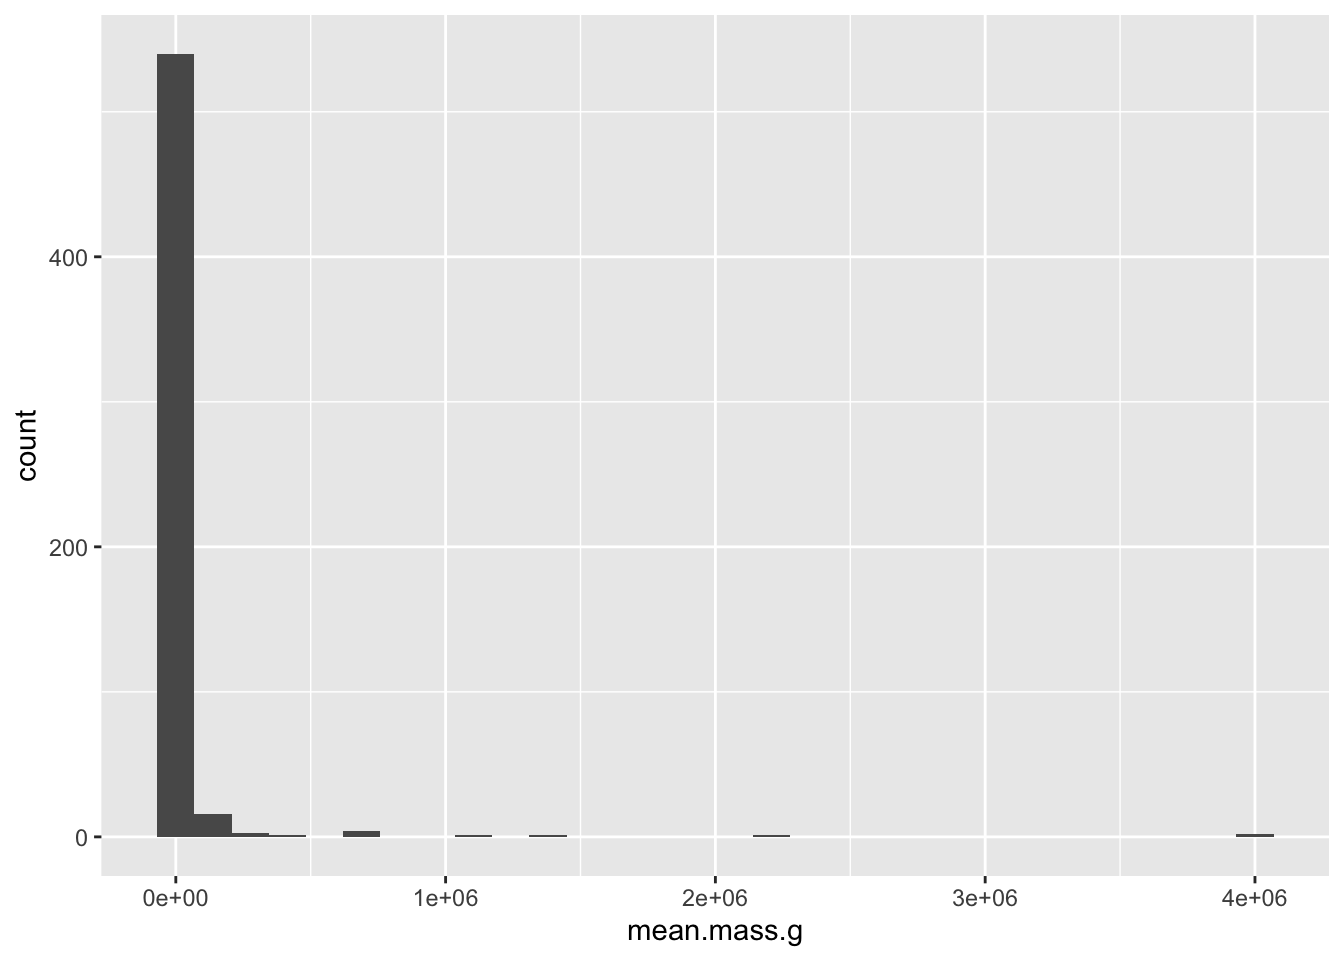
\includegraphics{practice_files/figure-latex/chart-mass-1.pdf}

The distribution becomes much clearer if we plot the logarithms of the masses,
which are helpfully precalculated in \texttt{log10.mass}:

\begin{Shaded}
\begin{Highlighting}[]
\NormalTok{ggplot2}\OperatorTok{::}\KeywordTok{ggplot}\NormalTok{(hra) }\OperatorTok{+}
\StringTok{  }\NormalTok{ggplot2}\OperatorTok{::}\KeywordTok{geom_histogram}\NormalTok{(}\DataTypeTok{mapping =} \KeywordTok{aes}\NormalTok{(}\DataTypeTok{x =}\NormalTok{ log10.mass))}
\end{Highlighting}
\end{Shaded}

\begin{verbatim}
`stat_bin()` using `bins = 30`. Pick better value with `binwidth`.
\end{verbatim}

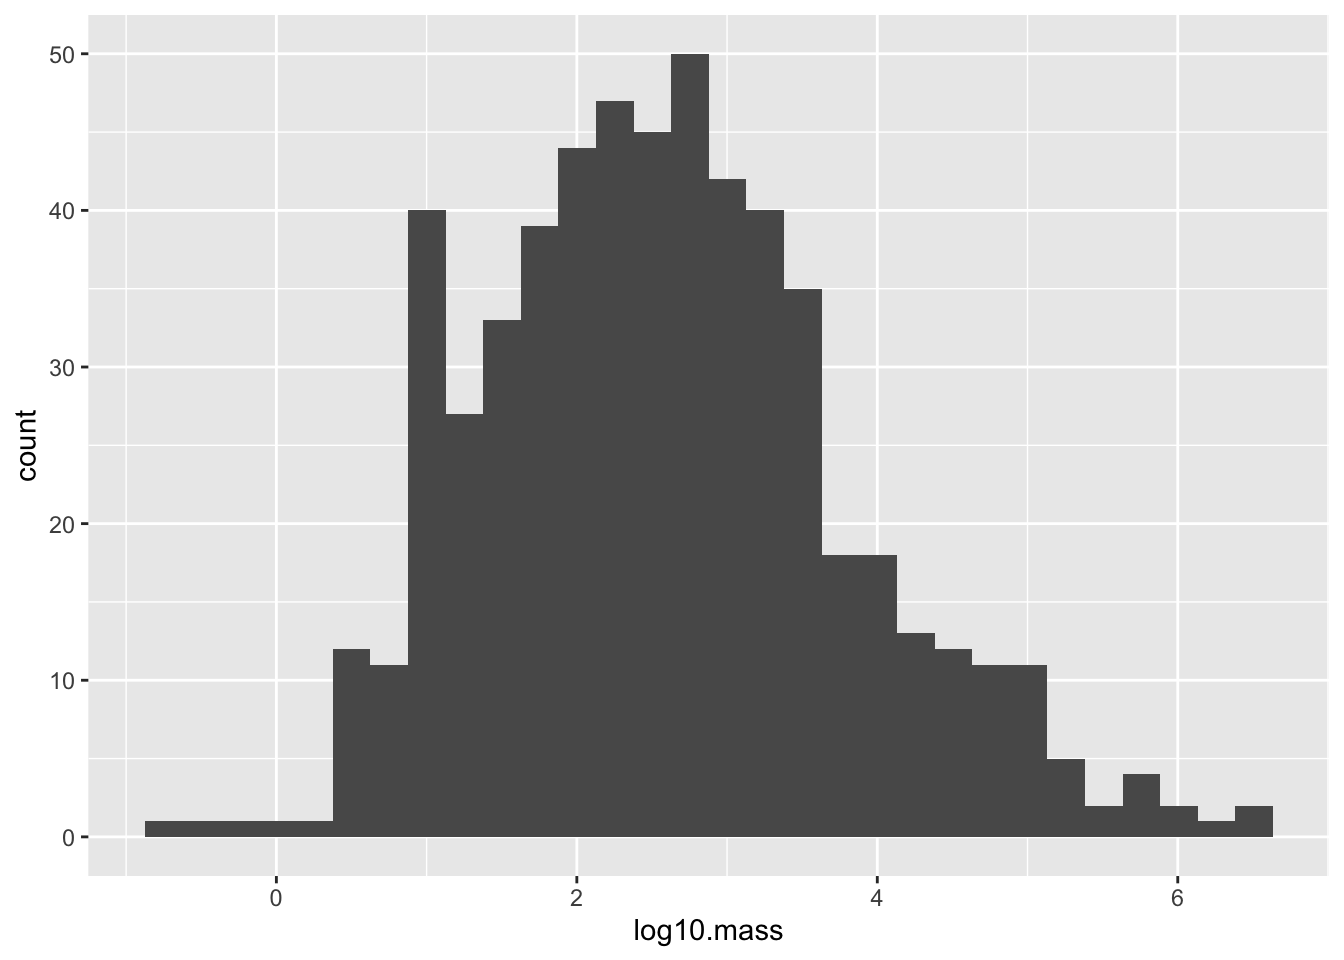
\includegraphics{practice_files/figure-latex/chart-log-mass-1.pdf}

Let's tidy that up a bit:

\begin{Shaded}
\begin{Highlighting}[]
\NormalTok{ggplot2}\OperatorTok{::}\KeywordTok{ggplot}\NormalTok{(hra) }\OperatorTok{+}
\StringTok{  }\NormalTok{ggplot2}\OperatorTok{::}\KeywordTok{geom_histogram}\NormalTok{(}\DataTypeTok{mapping =} \KeywordTok{aes}\NormalTok{(}\DataTypeTok{x =}\NormalTok{ log10.mass), }\DataTypeTok{bins =} \DecValTok{100}\NormalTok{) }\OperatorTok{+}
\StringTok{  }\NormalTok{ggplot2}\OperatorTok{::}\KeywordTok{ggtitle}\NormalTok{(}\StringTok{"Frequency of Species Masses"}\NormalTok{) }\OperatorTok{+}
\StringTok{  }\NormalTok{ggplot2}\OperatorTok{::}\KeywordTok{xlab}\NormalTok{(}\StringTok{"Log10 of Mass"}\NormalTok{) }\OperatorTok{+}
\StringTok{  }\NormalTok{ggplot2}\OperatorTok{::}\KeywordTok{ylab}\NormalTok{(}\StringTok{"Number of Species"}\NormalTok{) }\OperatorTok{+}
\StringTok{  }\NormalTok{ggplot2}\OperatorTok{::}\KeywordTok{theme_minimal}\NormalTok{()}
\end{Highlighting}
\end{Shaded}

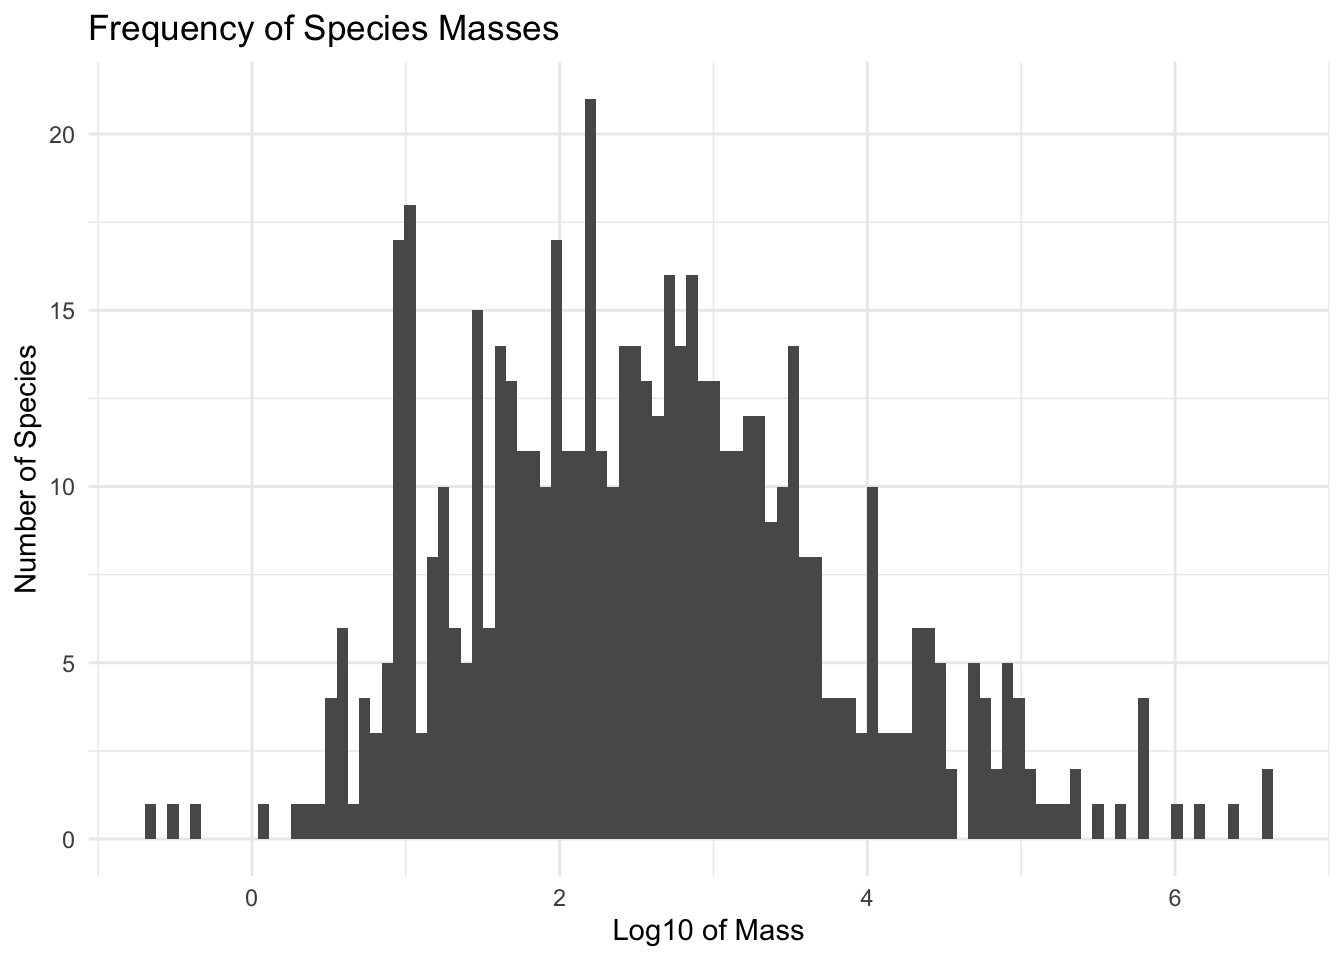
\includegraphics{practice_files/figure-latex/change-visual-1.pdf}

How are mass and home range area related?

\begin{Shaded}
\begin{Highlighting}[]
\NormalTok{ggplot2}\OperatorTok{::}\KeywordTok{ggplot}\NormalTok{(hra) }\OperatorTok{+}
\StringTok{  }\NormalTok{ggplot2}\OperatorTok{::}\KeywordTok{geom_point}\NormalTok{(}\DataTypeTok{mapping =} \KeywordTok{aes}\NormalTok{(}\DataTypeTok{x =}\NormalTok{ log10.mass, }\DataTypeTok{y =}\NormalTok{ log10.hra))}
\end{Highlighting}
\end{Shaded}

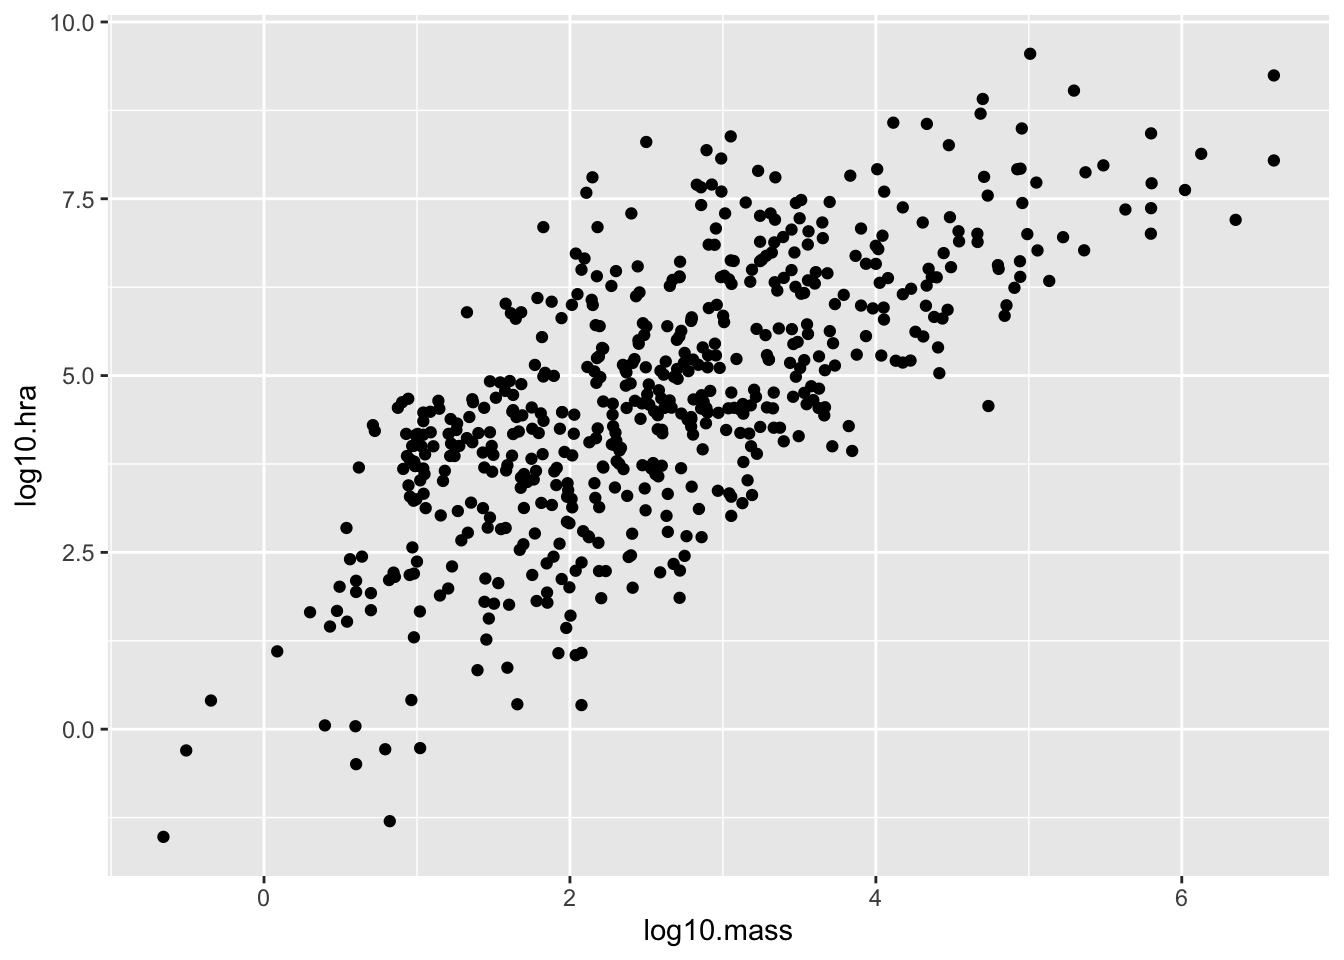
\includegraphics{practice_files/figure-latex/scatterplot-1.pdf}

Does the relationship depend on the class of animal?
(Here, we use the word ``class'' in the biological sense:
the class ``aves'' is birds.)

\begin{Shaded}
\begin{Highlighting}[]
\NormalTok{hra }\OperatorTok
\StringTok{  }\NormalTok{dplyr}\OperatorTok{::}\KeywordTok{mutate}\NormalTok{(}\DataTypeTok{class_fct =} \KeywordTok{as.factor}\NormalTok{(class)) }\OperatorTok
\StringTok{  }\NormalTok{ggplot2}\OperatorTok{::}\KeywordTok{ggplot}\NormalTok{(}\DataTypeTok{mapping =} \KeywordTok{aes}\NormalTok{(}\DataTypeTok{x =}\NormalTok{ log10.mass, }\DataTypeTok{y =}\NormalTok{ log10.hra, }\DataTypeTok{color =}\NormalTok{ class_fct)) }\OperatorTok{+}
\StringTok{  }\NormalTok{ggplot2}\OperatorTok{::}\KeywordTok{geom_point}\NormalTok{(}\DataTypeTok{alpha =} \FloatTok{0.5}\NormalTok{)}
\end{Highlighting}
\end{Shaded}

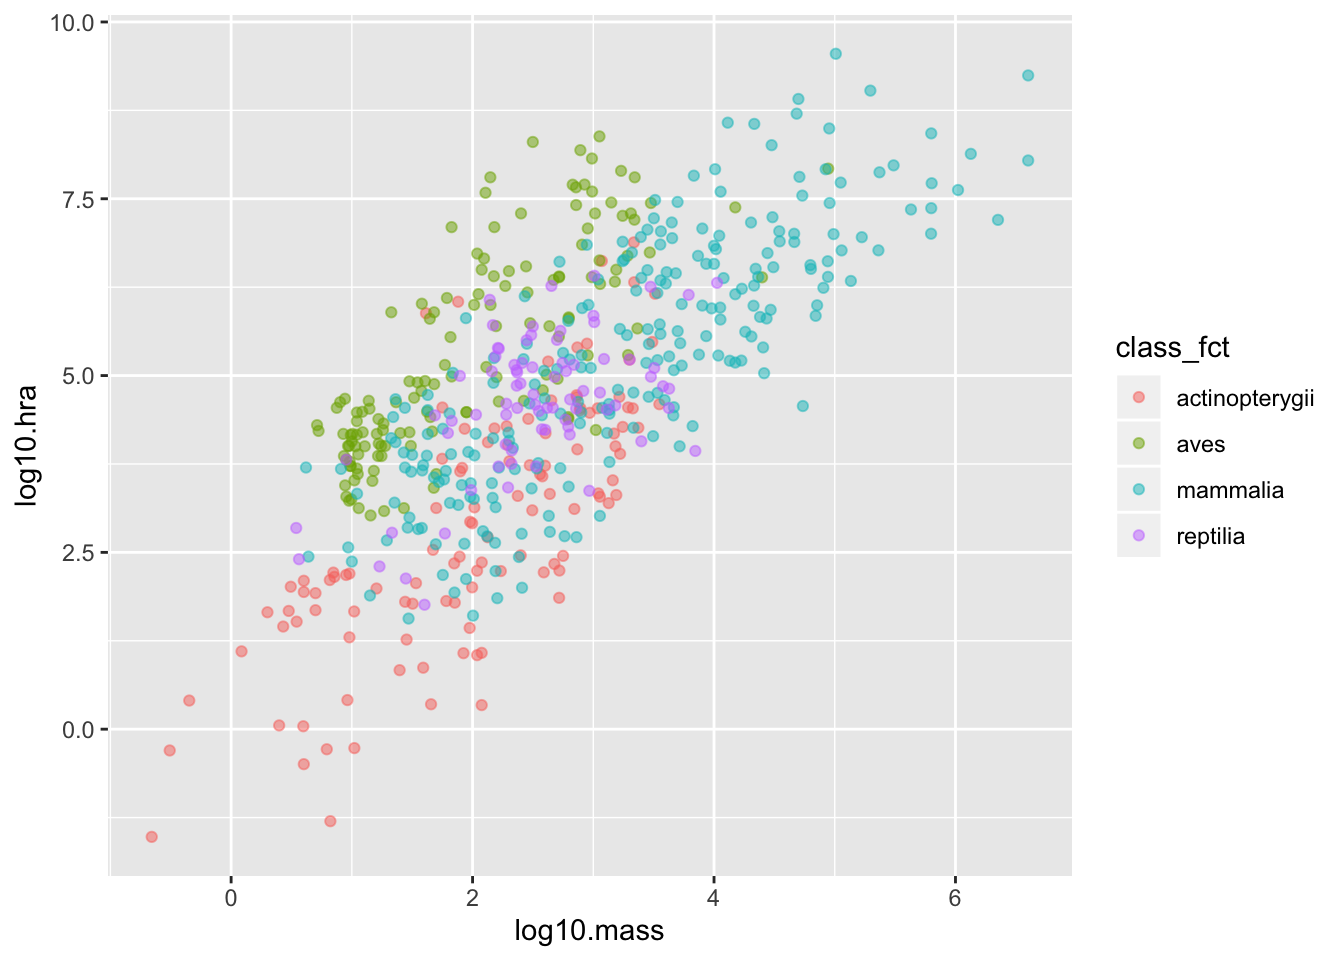
\includegraphics{practice_files/figure-latex/colorize-scatterplot-1.pdf}

\begin{quote}
*What's a Factor?

The code above creates a new column \texttt{class\_fct}
by converting the text values in \texttt{class} to a \href{glossary.html\#factor}{factor}.
Other languages call this an enumeration:
we will discuss factors in more detail in Chapter~\ref{debt}.
\end{quote}

Our chart may be clearer if we display the \href{glossary.html\#facet}{facets} separately:

\begin{Shaded}
\begin{Highlighting}[]
\NormalTok{hra }\OperatorTok
\StringTok{  }\NormalTok{dplyr}\OperatorTok{::}\KeywordTok{mutate}\NormalTok{(}\DataTypeTok{class_fct =} \KeywordTok{as.factor}\NormalTok{(class)) }\OperatorTok
\StringTok{  }\NormalTok{ggplot2}\OperatorTok{::}\KeywordTok{ggplot}\NormalTok{(}\DataTypeTok{mapping =} \KeywordTok{aes}\NormalTok{(}\DataTypeTok{x =}\NormalTok{ log10.mass, }\DataTypeTok{y =}\NormalTok{ log10.hra, }\DataTypeTok{color =}\NormalTok{ class_fct)) }\OperatorTok{+}
\StringTok{  }\NormalTok{ggplot2}\OperatorTok{::}\KeywordTok{geom_point}\NormalTok{(}\DataTypeTok{alpha =} \FloatTok{0.5}\NormalTok{) }\OperatorTok{+}
\StringTok{  }\NormalTok{ggplot2}\OperatorTok{::}\KeywordTok{facet_wrap}\NormalTok{(}\OperatorTok{~}\NormalTok{class_fct)}
\end{Highlighting}
\end{Shaded}

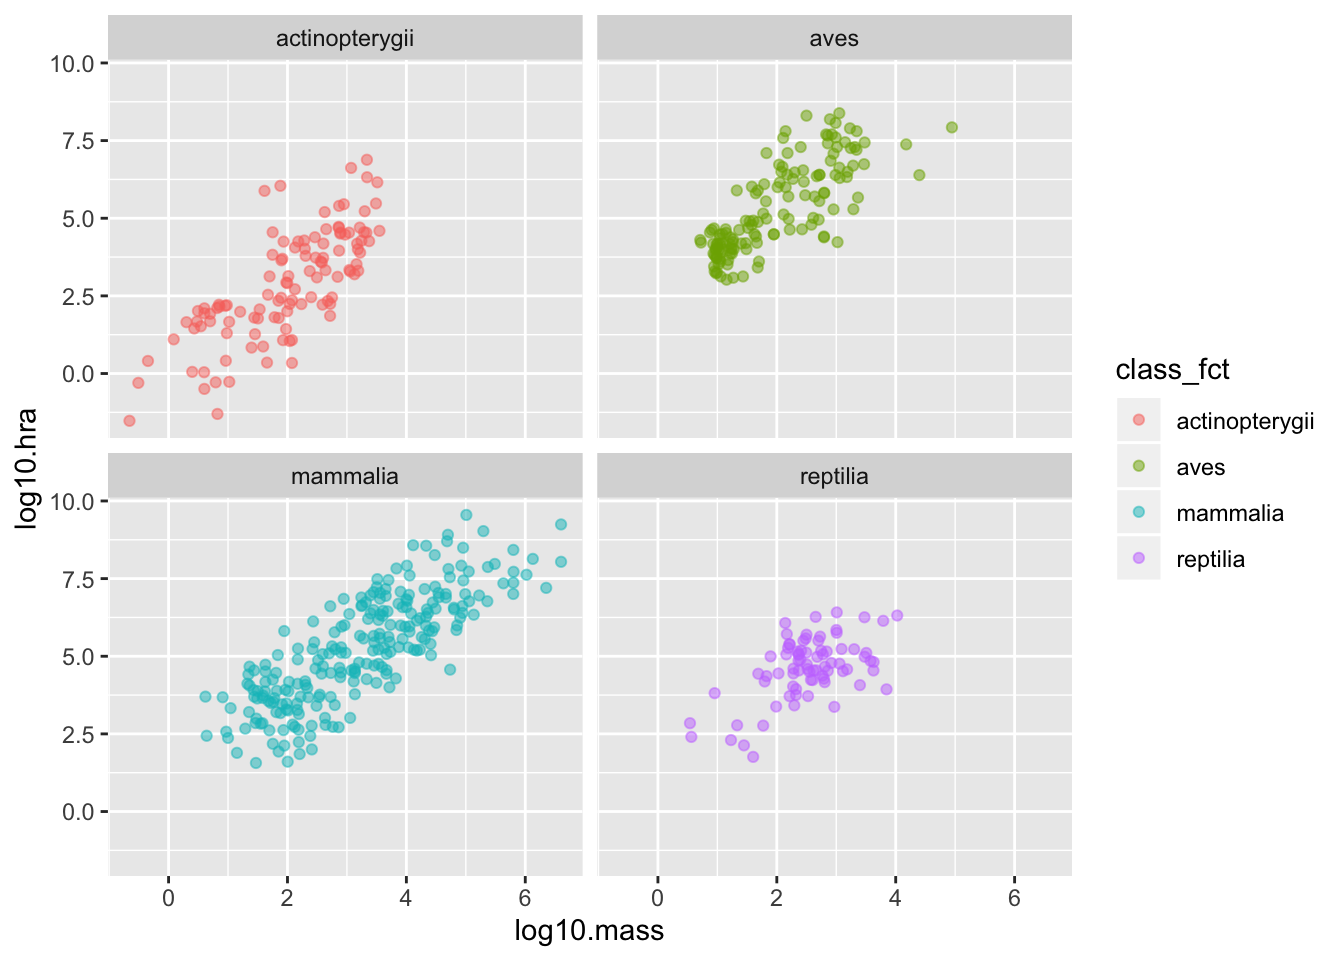
\includegraphics{practice_files/figure-latex/facet-plot-1.pdf}

If we want to look at the mass-area relationship more closely for birds,
we can construct a regression line:

\begin{Shaded}
\begin{Highlighting}[]
\NormalTok{hra }\OperatorTok
\StringTok{  }\NormalTok{dplyr}\OperatorTok{::}\KeywordTok{filter}\NormalTok{(class }\OperatorTok{==}\StringTok{ "aves"}\NormalTok{) }\OperatorTok
\StringTok{  }\NormalTok{ggplot2}\OperatorTok{::}\KeywordTok{ggplot}\NormalTok{(}\DataTypeTok{mapping =} \KeywordTok{aes}\NormalTok{(}\DataTypeTok{x =}\NormalTok{ log10.mass, }\DataTypeTok{y =}\NormalTok{ log10.hra)) }\OperatorTok{+}
\StringTok{  }\NormalTok{ggplot2}\OperatorTok{::}\KeywordTok{geom_point}\NormalTok{(}\DataTypeTok{alpha =} \FloatTok{0.5}\NormalTok{) }\OperatorTok{+}
\StringTok{  }\NormalTok{ggplot2}\OperatorTok{::}\KeywordTok{geom_smooth}\NormalTok{(}\DataTypeTok{method =}\NormalTok{ lm, }\DataTypeTok{color =} \StringTok{'red'}\NormalTok{)}
\end{Highlighting}
\end{Shaded}

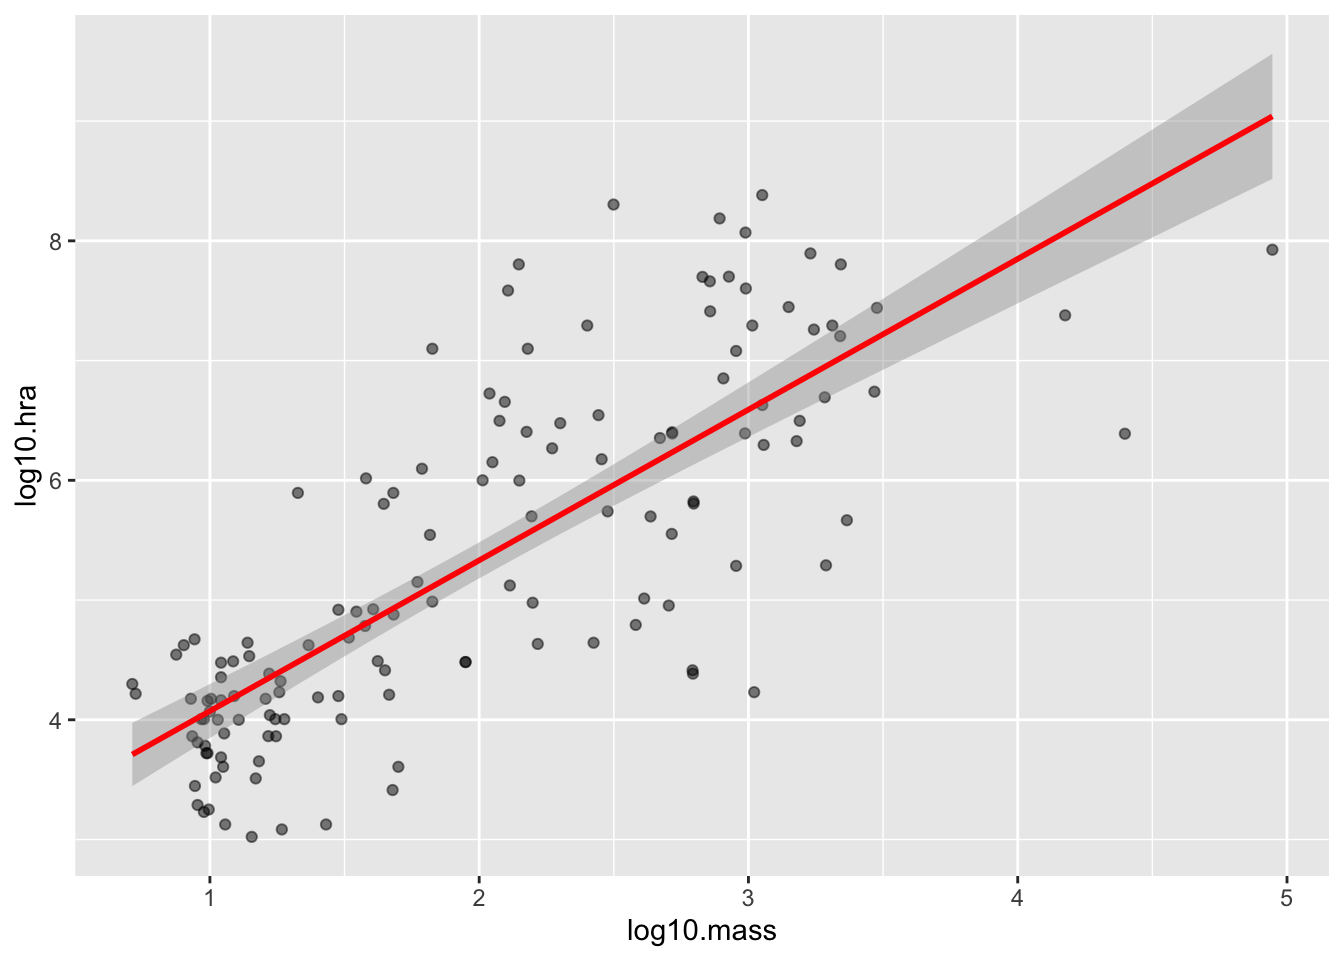
\includegraphics{practice_files/figure-latex/fit-line-1.pdf}

Drilling down even further,
we can create a violin plot of mass by order for the birds
(where ``order'' is the biological division below ``class''):

\begin{Shaded}
\begin{Highlighting}[]
\NormalTok{hra }\OperatorTok
\StringTok{  }\NormalTok{dplyr}\OperatorTok{::}\KeywordTok{filter}\NormalTok{(class }\OperatorTok{==}\StringTok{ "aves"}\NormalTok{) }\OperatorTok
\StringTok{  }\NormalTok{dplyr}\OperatorTok{::}\KeywordTok{mutate}\NormalTok{(}\DataTypeTok{order_fct =} \KeywordTok{as.factor}\NormalTok{(order)) }\OperatorTok
\StringTok{  }\NormalTok{ggplot2}\OperatorTok{::}\KeywordTok{ggplot}\NormalTok{(}\DataTypeTok{mapping =} \KeywordTok{aes}\NormalTok{(}\DataTypeTok{x =}\NormalTok{ order_fct, }\DataTypeTok{y =}\NormalTok{ log10.mass, }\DataTypeTok{color =}\NormalTok{ order_fct)) }\OperatorTok{+}
\StringTok{  }\NormalTok{ggplot2}\OperatorTok{::}\KeywordTok{geom_violin}\NormalTok{()}
\end{Highlighting}
\end{Shaded}

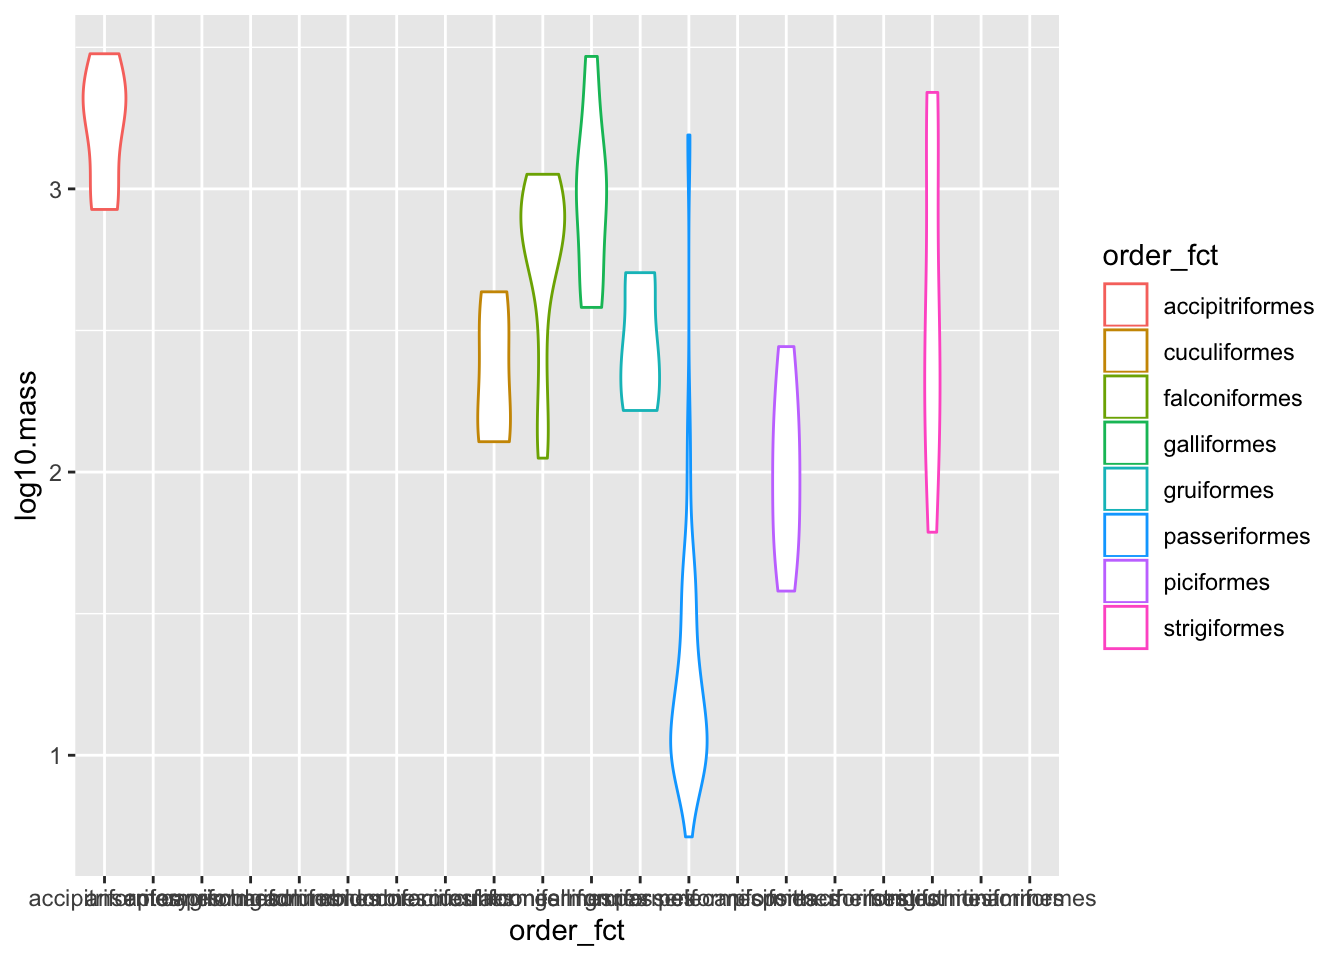
\includegraphics{practice_files/figure-latex/violin-plot-1.pdf}

Changing just one line gives us a box plot instead:

\begin{Shaded}
\begin{Highlighting}[]
\NormalTok{hra }\OperatorTok
\StringTok{  }\NormalTok{dplyr}\OperatorTok{::}\KeywordTok{filter}\NormalTok{(class }\OperatorTok{==}\StringTok{ "aves"}\NormalTok{) }\OperatorTok
\StringTok{  }\NormalTok{dplyr}\OperatorTok{::}\KeywordTok{mutate}\NormalTok{(}\DataTypeTok{order_fct =} \KeywordTok{as.factor}\NormalTok{(order)) }\OperatorTok
\StringTok{  }\NormalTok{ggplot2}\OperatorTok{::}\KeywordTok{ggplot}\NormalTok{(}\DataTypeTok{mapping =} \KeywordTok{aes}\NormalTok{(}\DataTypeTok{x =}\NormalTok{ order_fct, }\DataTypeTok{y =}\NormalTok{ log10.mass, }\DataTypeTok{color =}\NormalTok{ order_fct)) }\OperatorTok{+}
\StringTok{  }\NormalTok{ggplot2}\OperatorTok{::}\KeywordTok{geom_boxplot}\NormalTok{()}
\end{Highlighting}
\end{Shaded}

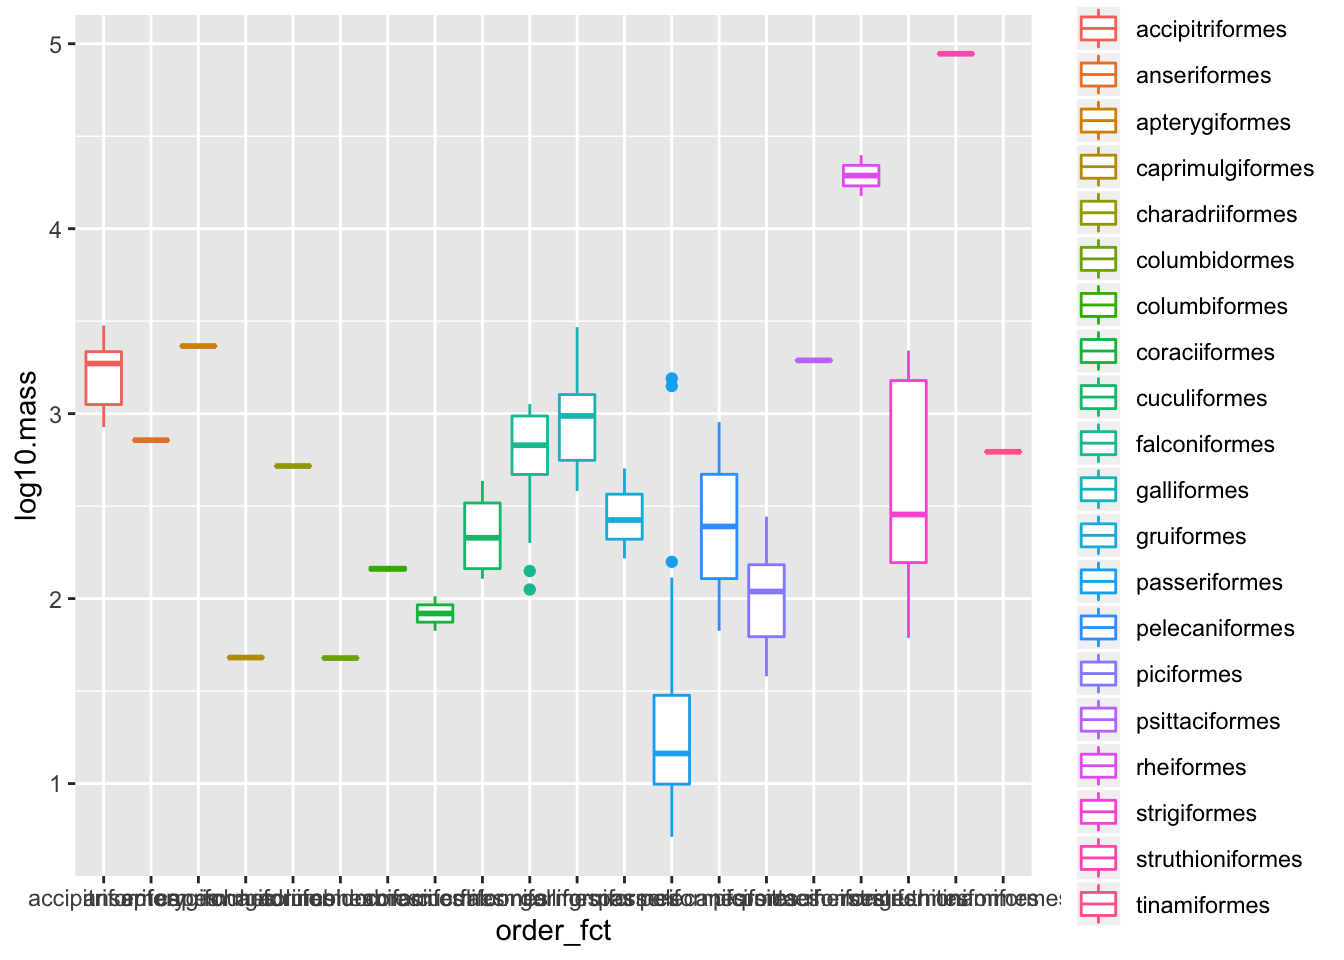
\includegraphics{practice_files/figure-latex/box-plot-1.pdf}

And if we want to save our chart to a file,
that's just one more call as well:

\begin{Shaded}
\begin{Highlighting}[]
\NormalTok{hra }\OperatorTok
\StringTok{  }\NormalTok{dplyr}\OperatorTok{::}\KeywordTok{filter}\NormalTok{(class }\OperatorTok{==}\StringTok{ "aves"}\NormalTok{) }\OperatorTok
\StringTok{  }\NormalTok{ggplot2}\OperatorTok{::}\KeywordTok{ggplot}\NormalTok{(}\DataTypeTok{mapping =} \KeywordTok{aes}\NormalTok{(}\DataTypeTok{x =}\NormalTok{ log10.mass, }\DataTypeTok{y =}\NormalTok{ log10.hra)) }\OperatorTok{+}
\StringTok{  }\NormalTok{ggplot2}\OperatorTok{::}\KeywordTok{geom_point}\NormalTok{(}\DataTypeTok{alpha =} \FloatTok{0.5}\NormalTok{) }\OperatorTok{+}
\StringTok{  }\NormalTok{ggplot2}\OperatorTok{::}\KeywordTok{geom_smooth}\NormalTok{(}\DataTypeTok{method =}\NormalTok{ lm, }\DataTypeTok{color =} \StringTok{'red'}\NormalTok{)}
\end{Highlighting}
\end{Shaded}

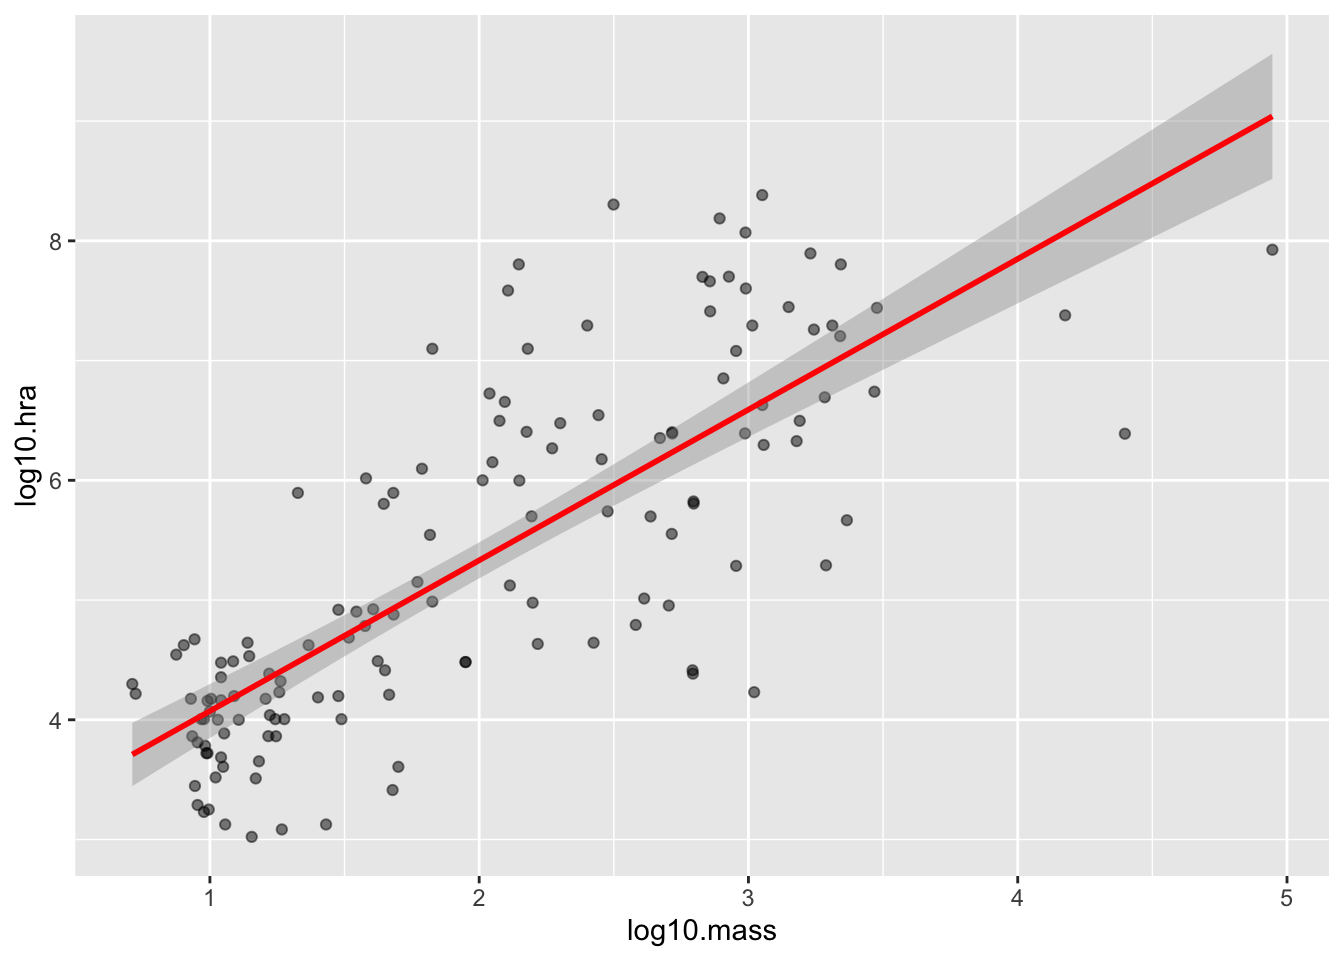
\includegraphics{practice_files/figure-latex/save-file-1.pdf}

\begin{Shaded}
\begin{Highlighting}[]
\KeywordTok{ggsave}\NormalTok{(}\StringTok{"/tmp/birds.png"}\NormalTok{)}
\end{Highlighting}
\end{Shaded}

\begin{verbatim}
Saving 6.5 x 4.5 in image
\end{verbatim}

\hypertarget{glossary}{%
\chapter{Glossary}\label{glossary}}

\begin{description}
\tightlist
\item[\textbf{Absolute row number}]
The sequential index of a row in a table,
regardless of what sections of the table is being displayed.
\item[\textbf{Aggregation}]
To combine many values into one,
e.g.,
by summing a set of numbers or concatenating a set of strings.
\item[\textbf{Alias}]
To have two (or more) references to the same physical data.
\item[\textbf{Anonymous function}]
A function that has not been assigned a name.
Anonymous functions are usually quite short,
and are usually defined where they are used,
e.g.,
as callbacks.
\item[\textbf{Attribute}]
A name-value pair associated with an object,
used to store metadata about the object
such as an array's dimensions.
\item[\textbf{Catch (exception)}]
To accept responsibility for handling an error
or other unexpected event.
R prefers ``\href{glossary.html\#handle-condition}{handling} a \href{glossary.html\#condition}{condition}''
to ``catching an \href{glossary.html\#exception}{exception}''.
\item[\textbf{Condition}]
An error or other unexpected event that disrupts the normal flow of control.
See also \href{glossary.html\#handle-condition}{handle}.
\item[\textbf{Constructor (class)}]
A function that creates an object of a particular class.
In the \href{glossary.html\#S3}{S3} object system,
constructors are a convention rather than a requirement.
\item[\textbf{Copy-on-modify}]
The practice of creating a new copy of \href{glossary.html\#alias}{aliased} data
whenever there is an attempt to modify it
so that each reference will believe theirs is the only one.
\item[\textbf{Double square brackets}]
An index enclosed in \texttt{{[}{[}...{]}{]}},
used to return a single value of the underlying type.
See also \href{glossary.html\#single-square-brackets}{single square brackets}.
\item[\textbf{Eager evaluation}]
Evaluating an expression as soon as it is formed.
\item[\textbf{Empty vector}]
A vector that contains no elements.
Empty vectors have a type such as logical or character,
and are \emph{not} the same as \href{glossary.html\#null}{null}.
\item[\textbf{Environment}]
A structure that stores a set of variable names and the values they refer to.
\item[\textbf{Error}]
The most severe type of built-in \href{glossary.html\#condition}{condition} in R.
\item[\textbf{Evaluating function}]
A function that takes arguments as values.
Most functions are evaluating functions.
\item[\textbf{Evaluation}]
The process of taking a complex expression such as \texttt{1+2*3/4}
and turning it into a single irreducible value.
\item[\textbf{Exception}]
An object containing information about an error,
or the condition that led to the error.
R prefers ``\href{glossary.html\#handle-condition}{handling} a \href{glossary.html\#condition}{condition}''
to ``\href{glossary.html\#catch-exception}{catching} an \href{glossary.html\#exception}{exception}''.
\item[\textbf{Filter}]
To choose a set of records according to the values they contain.
\item[\textbf{Fully qualified name}]
An unambiguous name of the form package::thing.
\item[\textbf{Functional programming}]
A style of programming in which functions transform data rather than modifying it.
Functional programming relies heavily on \href{glossary.html\#higher-order-function}{higher-order functions}.
\item[\textbf{Generic function}]
A collection of functions with similar purpose,
each operating on a different class of data.
\item[\textbf{Global environment}]
The \href{glossary.html\#environment}{environment} that holds top-level definitions in R,
e.g.,
those written directly in the interpreter.
\item[\textbf{Group}]
To divide data into subsets according to some criteria
while leaving records in a single structure.
\item[\textbf{Handle (a condition)}]
To accept responsibility for handling an error
or other unexpected event.
R prefers ``handling a \href{glossary.html\#condition}{condition}''
to ``\href{glossary.html\#catch-exception}{catching} an \href{glossary.html\#exception}{exception}''.
\item[\textbf{Helper (class)}]
In \href{glossary.html\#S3}{S3},
a function that \href{glossary.html\#constructor}{constructs} and \href{glossary.html\#validator}{validates}
an instance of a class.
\item[\textbf{Heterogeneous}]
Potentially containing data of different types.
Most vectors in R are \href{glossary.html\#homogeneous}{homogeneous},
but lists can be heterogeneous.
\item[\textbf{Higher-order function}]
A function that takes one or more other functions as parameters.
Higher-order functions such as \texttt{map} are commonly used in \href{glossary.html\#functional-programming}{functional programming}.
\item[\textbf{Homogeneous}]
Containing data of only a single type.
Most vectors in R are homogeneous.
\item[\textbf{Hubris}]
Excessive pride or self-confidence.
See also \href{glossary.html\#unit-test}{unit test} (lack of).
\item[\textbf{ISO3 country code}]
A three-letter code defined by ISO 3166-1 that identifies a specific country,
dependent territory,
or other geopolitical entity.
\item[\textbf{Lazy evaluation}]
Delaying evaluation of an expression until the value is actually needed
(or at least until after the point where it is first encountered).
\item[\textbf{List}]
A vector that can contain values of many different types.
\item[\textbf{List comprehension}]
An expression that generates a new list from an existing one via an implicit loop.
\item[\textbf{Logical indexing}]
To index a vector or other structure with a vector of Booleans,
keeping only the values that correspond to true values.
\item[\textbf{Message}]
The least severe type of built-in \href{glossary.html\#condition}{condition} in R.
\item[\textbf{Method}]
An implementation of a \href{glossary.html\#generic-function}{generic function}
that handles objects of a specific class.
\item[\textbf{NA}]
A special value used to represent data that is Not Available.
\item[\textbf{Name collision}]
A situation in which the same name has been used in two different packages
which are then used together,
leading to ambiguity.
\item[\textbf{Named list}]
FIXME
\item[\textbf{Negative selection}]
To specify the elements of a vector or other data structure that \emph{aren't} desired
by negating their indices.
\item[\textbf{Null}]
A special value used to represent a missing object.
\texttt{NULL} is not the same as \texttt{NA},
and neither is the same as an \href{glossary.html\#empty-vector}{empty vector}.
\item[\textbf{Package}]
A collection of code, data, and documentation
that can be distributed and re-used.
\item[\textbf{Pipe operator}]
The \texttt{\%\textgreater{}\%} used to make the output of one function the input of the next.
\item[\textbf{Prefix operator}]
An operator that comes before the single value it operates on,
such as the \texttt{-} in \texttt{-(a*b)}.
\item[\textbf{Promise}]
A data structure used to record an unevaluated expression for lazy evaluation.
\item[\textbf{Pull indexing}]
Vectorized indexing in which the value at location \emph{i} in the index vector
specifies which element of the source vector
is being pulled into that location in the result vector,
i.e., \texttt{result{[}i{]}\ =\ source{[}index{[}i{]}{]}}.
See also \href{glossary.html\#push-indexing}{push indexing}.
\item[\textbf{Push indexing}]
Vectorized indexing in which the value at location \emph{i} in the index vector
specifies an element of the result vector that gets the corresponding element of the source vector,
i.e., \texttt{result{[}index{[}i{]}{]}\ =\ source{[}i{]}}.
Push indexing can easily produce gaps and collisions.
See also \href{glossary.html\#pull-indexing}{pull indexing}.
\item[\textbf{Quosure}]
A data structure containing an unevaluated expression and its environment.
\item[\textbf{Quoting function}]
A function that is passed expressions rather than the values of those expressions.
\item[\textbf{Raise (exception)}]
A way of indicating that something has gone wrong in a program,
or that some other unexpected event has occurred.
R prefers ``\href{glossary.html\#signal-condition}{signalling} a \href{glossary.html\#condition}{condition}''
to ``raising an \href{glossary.html\#exception}{exception}''.
\item[\textbf{Range expression}]
An expression of the form low:high
that is transformed a sequence of consecutive integers.
\item[\textbf{Reactive programming}]
A style of programming in which actions are triggered by external events.
\item[\textbf{Reactive variable}]
A variable whose value is automatically updated when some other value or values change.
\item[\textbf{Recycle}]
To re-use values from a shorter vector in order to generate
a sequence of the same length as a longer one.
\item[\textbf{Regular expression}]
A pattern for matching text.
Regular expressions are themselves written as text,
which makes them as cryptic as they are powerful.
\item[\textbf{Relative row number}]
The index of a row in a displayed portion of a table,
which may or may not be the same as the \href{glossary.html\#absolute-row-number}{absolut row number}
within the table.
\item[\textbf{Repository}]
The place where a version control system stores a project's files
and the metadata used to record their history.
\item[\textbf{S3}]
A framework for object-oriented programming in R.
\item[\textbf{Scalar}]
A single value of a particular type, such as 1 or ``a''.
Scalars don't really exist in R;
values that appear to be scalars are actually vectors of unit length.
\item[\textbf{Select}]
To choose entire columns from a table by name or location.
\item[\textbf{Setup (testing)}]
Code that is automatically run once before each \href{glossary.html\#unit-test}{unit test}.
\item[\textbf{Signal (a condition)}]
A way of indicating that something has gone wrong in a program,
or that some other unexpected event has occurred.
R prefers ``signalling a \href{glossary.html\#condition}{condition}''
to ``\href{glossary.html\#raise-exception}{raising} an \href{glossary.html\#exception}{exception}''.
\item[\textbf{Single square brackets}]
An index enclosed in \texttt{{[}...{]}},
used to select a structure from another structure.
See also \href{glossary.html\#double-square-brackets}{double square brackets}.
\item[\textbf{Storage allocation}]
Setting aside a block of memory for future use.
\item[\textbf{Teardown (testing)}]
Code that is automatically run once after each \href{glossary.html\#unit-test}{unit test}.
\item[\textbf{Test fixture}]
The data structures, files, or other artefacts on which a \href{glossary.html\#unit-test}{unit test} operates.
\item[\textbf{Test runner}]
A software tool that finds and runs \href{glossary.html\#unit-test}{unit tests}.
\item[\textbf{Tibble}]
A modern replacement for R's data frame,
which stores tabular data in columns and rows,
defined and used in the \href{glossary.html\#tidyverse}{tidyverse}.
\item[\textbf{Tidyverse}]
A collection of R packages for operating on tabular data in consistent ways.
\item[\textbf{Unit test}]
A function that tests one aspect or property of a piece of software.
\item[\textbf{Validator (class)}]
A function that checks the consistency of an \href{glossary.html\#S3}{S3} object.
\item[\textbf{Variable arguments}]
In a function,
the ability to take any number of arguments.
R uses \texttt{...} to capture the ``extra'' arguments.
\item[\textbf{Vector}]
A sequence of values,
usually of \href{glossary.html\#homogeneous}{homogeneous} type.
Vectors are \emph{the} fundamental data structure in R;
\href{glossary.html\#scalar}{scalars} are actually vectors of unit length.
\item[\textbf{Vectorize}]
To write code so that operations are performed on entire vectors,
rather than element-by-element within loops.
\item[\textbf{Warning}]
A built-in \href{glossary.html\#condition}{condition} in R of middling severity.
\item[\textbf{Widget}]
An interactive control element in an user interface.
\end{description}

\hypertarget{keypoints}{%
\chapter{Key Points}\label{keypoints}}

\hypertarget{simple-beginnings}{%
\section{Simple Beginnings}\label{simple-beginnings}}

\begin{itemize}
\tightlist
\item
  Use \texttt{print(expression)} to print the value of a single expression.
\item
  Variable names may include letters, digits, \texttt{.}, and \texttt{\_}, but \texttt{.} should be avoided, as it sometimes has special meaning.
\item
  R's atomic data types include logical, integer, double (also called numeric), and character.
\item
  R stores collections in homogeneous vectors of atomic types, or in heterogeneous lists.
\item
  `Scalars' in R are actually vectors of length 1.
\item
  Vectors and lists are created using the function \texttt{c(...)}.
\item
  Vector indices from 1 to length(vector) select single elements.
\item
  Negative indices to vectors deselect elements from the result.
\item
  The index 0 on its own selects no elements, creating a vector or list of length 0.
\item
  The expression \texttt{low:high} creates the vector of integers from \texttt{low} to \texttt{high} inclusive.
\item
  Subscripting a vector with a vector of numbers selects the elements at those locations (possibly with repeats).
\item
  Subscripting a vector with a vector of logicals selects elements where the indexing vector is \texttt{TRUE}.
\item
  Values from short vectors (such as `scalars') are repeated to match the lengths of longer vectors.
\item
  The special value \texttt{NA} represents missing values, and (almost all) operations involving \texttt{NA} produce \texttt{NA}.
\item
  The special values \texttt{NULL} represents a nonexistent vector, which is not the same as a vector of length 0.
\item
  A list is a heterogeneous vector capable of storing values of any type (including other lists).
\item
  Indexing with \texttt{{[}} returns a structure of the same type as the structure being indexed (e.g., returns a list when applied to a list).
\item
  Indexing with \texttt{{[}{[}} strips away one level of structure (i.e., returns the indicated element without any wrapping).
\item
  Use \texttt{list(\textquotesingle{}name\textquotesingle{}\ =\ value,\ ...)} to name the elements of a list.
\item
  Use either \texttt{L{[}\textquotesingle{}name\textquotesingle{}{]}} or \texttt{L\$name} to access elements by name.
\item
  Use back-quotes around the name with \texttt{\$} notation if the name is not a legal R variable name.
\item
  Use \texttt{matrix(values,\ nrow\ =\ N)} to create a matrix with \texttt{N} rows containing the given values.
\item
  Use \texttt{m{[}i,\ j{]}} to get the value at the i'th row and j'th column of a matrix.
\item
  Use \texttt{m{[}i,{]}} to get a vector containing the values in the i'th row of a matrix.
\item
  Use \texttt{m{[},j{]}} to get a vector containing the values in the j'th column of a matrix.
\item
  Use \texttt{for\ (loop\_variable\ in\ collection)\{\ ...body...\ \}} to create a loop.
\item
  Use \texttt{if\ (expression)\ \{\ ...body...\ \}\ else\ if\ (expression)\ \{\ ...body...\ \}\ else\ \{\ ...body...\ \}} to create conditionals.
\item
  Expression conditions must have length 1; use \texttt{any(...)} and \texttt{all(...)} to collapse logical vectors to single values.
\item
  Use \texttt{function(...arguments...)\ \{\ ...body...\ \}} to create a function.
\item
  Use variable \textless{}- function(\ldots{}arguments\ldots{}) \{ \ldots{}body\ldots{} \}` to create a function and give it a name.
\item
  The body of a function can be a single expression or a block in curly braces.
\item
  The last expression evaluated in a function is returned as its result.
\item
  Use \texttt{return(expression)} to return a result early from a function.
\end{itemize}

\hypertarget{the-tidyverse}{%
\section{The Tidyverse}\label{the-tidyverse}}

\begin{itemize}
\tightlist
\item
  \texttt{install.packages(\textquotesingle{}name\textquotesingle{})} installs packages.
\item
  \texttt{library(name)} (without quoting the name) loads a package.
\item
  \texttt{library(tidyverse)} loads the entire collection of tidyverse libraries at once.
\item
  \texttt{read\_csv(filename)} reads CSV files that use the string `NA' to represent missing values.
\item
  \texttt{read\_csv} infers each column's data types based on the first thousand values it reads.
\item
  A tibble is the tidyverse's version of a data frame, which represents tabular data.
\item
  \texttt{head(tibble)} and \texttt{tail(tibble)} inspect the first and last few rows of a tibble.
\item
  \texttt{summary(tibble)} displays a summary of a tibble's structure and values.
\item
  \texttt{tibble\$column} selects a column from a tibble, returning a vector as a result.
\item
  \texttt{tibble{[}\textquotesingle{}column\textquotesingle{}{]}} selects a column from a tibble, returning a tibble as a result.
\item
  \texttt{tibble{[},c{]}} selects column \texttt{c} from a tibble, returning a tibble as a result.
\item
  \texttt{tibble{[}r,{]}} selects row \texttt{r} from a tibble, returning a tibble as a result.
\item
  Use ranges and logical vectors as indices to select multiple rows/columns or specific rows/columns from a tibble.
\item
  \texttt{tibble{[}{[}c{]}{]}} selects column \texttt{c} from a tibble, returning a vector as a result.
\item
  \texttt{min(...)}, \texttt{mean(...)}, \texttt{max(...)}, and \texttt{std(...)} calculates the minimum, mean, maximum, and standard deviation of data.
\item
  These aggregate functions include \texttt{NA}s in their calculations, and so will produce \texttt{NA} if the input data contains any.
\item
  Use \texttt{func(data,\ na.rm\ =\ TRUE)} to remove \texttt{NA}s from data before calculations are done (but make sure this is statistically justified).
\item
  \texttt{filter(tibble,\ condition)} selects rows from a tibble that pass a logical test on their values.
\item
  \texttt{arrange(tibble,\ column)} or \texttt{arrange(desc(column))} arrange rows according to values in a column (the latter in descending order).
\item
  \texttt{select(tibble,\ column,\ column,\ ...)} selects columns from a tibble.
\item
  \texttt{select(tibble,\ -column)} selects \emph{out} a column from a tibble.
\item
  \texttt{mutate(tibble,\ name\ =\ expression,\ name\ =\ expression,\ ...)} adds new columns to a tibble using values from existing columns.
\item
  \texttt{group\_by(tibble,\ column,\ column,\ ...)} groups rows that have the same values in the specified columns.
\item
  \texttt{summarize(tibble,\ name\ =\ expression,\ name\ =\ expression)} aggregates tibble values (by groups if the rows have been grouped).
\item
  \texttt{tibble\ \%\textgreater{}\%\ function(arguments)} performs the same operation as \texttt{function(tibble,\ arguments)}.
\item
  Use \texttt{\%\textgreater{}\%} to create pipelines in which the left side of each \texttt{\%\textgreater{}\%} becomes the first argument of the next stage.
\end{itemize}

\hypertarget{creating-packages}{%
\section{Creating Packages}\label{creating-packages}}

\begin{itemize}
\tightlist
\item
  Develop data-cleaning scripts one step at a time, checking intermediate results carefully.
\item
  Use \texttt{read\_csv} to read CSV-formatted tabular data into a tibble.
\item
  Use the \texttt{skip} and \texttt{na} parameters of \texttt{read\_csv} to skip rows and interpret certain values as \texttt{NA}.
\item
  Use \texttt{str\_replace} to replace portions of strings that match patterns with new strings.
\item
  Use \texttt{is.numeric} to test if a value is a number and \texttt{as.numeric} to convert it to a number.
\item
  Use \texttt{map} to apply a function to every element of a vector in turn.
\item
  Use \texttt{map\_dfc} and \texttt{map\_dfr} to map functions across the columns and rows of a tibble.
\item
  Pre-allocate storage in a list for each result from a loop and fill it in rather than repeatedly extending the list.
\item
  An R package can contain code, data, and documentation.
\item
  R code is distributed as compiled bytecode in packages, not as source.
\item
  R packages are almost always distributed through CRAN, the Comprehensive R Archive Network.
\item
  Most of a project's metadata goes in a file called \texttt{DESCRIPTION}.
\item
  Metadata related to imports and exports goes in a file called \texttt{NAMESPACE}.
\item
  Add patterns to a file called \texttt{.Rbuildignore} to ignore files or directories when building a project.
\item
  All source code for a package must go in the \texttt{R} sub-directory.
\item
  \texttt{library} calls in a package's source code will \emph{not} be executed as the package is loaded after distribution.
\item
  Data can be included in a package by putting it in the \texttt{data} sub-directory.
\item
  Data must be in \texttt{.rda} format in order to be loaded as part of a package.
\item
  Data in other formats can be put in the \texttt{inst/extdata} directory, and will be installed when the package is installed.
\item
  Add comments starting with \texttt{\#\textquotesingle{}} to an R file to document functions.
\item
  Use roxygen2 to extract these comments to create manual pages in the \texttt{man} directory.
\item
  Use \texttt{@export} directives in roxygen2 comment blocks to make functions visible outside a package.
\item
  Add required libraries to the \texttt{Imports} section of the \texttt{DESCRIPTION} file to indicate that your package depends on them.
\item
  Use \texttt{package::function} to access externally-defined functions inside a package.
\item
  Alternatively, add \texttt{@import} directives to roxygen2 comment blocks to make external functions available inside the package.
\item
  Import \texttt{.data} from \texttt{rlang} and use \texttt{.data\$column} to refer to columns instead of using bare column names.
\item
  Create a file called R/package.R and document \texttt{NULL} to document the package as a whole.
\item
  Create a file called R/dataset.R and document the string `dataset' to document a dataset.
\end{itemize}

\hypertarget{non-standard-evaluation}{%
\section{Non-Standard Evaluation}\label{non-standard-evaluation}}

\begin{itemize}
\tightlist
\item
  R uses lazy evaluation: expressions are evaluated when their values are needed, not before.
\item
  Use \texttt{expr} to create an expression without evaluating it.
\item
  Use \texttt{eval} to evaluate an expression in the context of some data.
\item
  Use \texttt{enquo} to create a quosure containing an unevaluated expression and its environment.
\item
  Use \texttt{quo\_get\_expr} to get the expression out of a quosure.
\item
  Use \texttt{!!} to splice the expression in a quosure into a function call.
\end{itemize}

\hypertarget{intellectual-debt}{%
\section{Intellectual Debt}\label{intellectual-debt}}

\begin{itemize}
\tightlist
\item
  Don't use \texttt{setwd}.
\item
  The formula operator \texttt{\textasciitilde{}} delays evaluation of its operand or operands.
\item
  \texttt{\textasciitilde{}} was created to allow users to pass formulas into functions, but is used more generally to delay evaluation.
\item
  Some tidyverse functions define \texttt{.} to be the whole data, \texttt{.x} and \texttt{.y} to be the first and second arguments, and \texttt{..N} to be the N'th argument.
\item
  These convenience parameters are primarily used when the data being passed to a pipelined function needs to go somewhere other than in the first parameter's slot.
\item
  `Copy-on-modify' means that data is aliased until something attempts to modify it, at which point it duplicated, so that data always appears to be unchanged.
\end{itemize}

\hypertarget{testing-and-error-handling}{%
\section{Testing and Error Handling}\label{testing-and-error-handling}}

\begin{itemize}
\tightlist
\item
  Operations signal conditions in R when errors occur.
\item
  The three built-in levels of conditions are messages, warnings, and errors.
\item
  Programs can signal these themselves using the functions \texttt{message}, \texttt{warning}, and \texttt{stop}.
\item
  Operations can be placed in a call to the function \texttt{try} to suppress errors, but this is a bad idea.
\item
  Operations can be placed in a call to the function \texttt{tryCatch} to handle errors.
\item
  Use testthat to write unit tests for R.
\item
  Put unit tests for an R package in the \texttt{tests/testthat} directory.
\item
  Put tests in files called test\_group.R and call them test\_something.
\item
  Use \texttt{test\_dir} to run tests from a particular that match a pattern.
\item
  Write tests for data transformation steps as well as library functions.
\end{itemize}

\hypertarget{advanced-topics}{%
\section{Advanced Topics}\label{advanced-topics}}

\begin{itemize}
\tightlist
\item
  The \texttt{reticulate} library allows R programs to access data in Python programs and vice versa.
\item
  Use \texttt{py.whatever} to access a top-level Python variable from R.
\item
  Use \texttt{r.whatever} to access a top-level R definition from Python.
\item
  R is always indexed from 1 (even in Python) and Python is always indexed from 0 (even in R).
\item
  Numbers in R are floating point by default, so use a trailing `L' to force a value to be an integer.
\item
  A Python script run from an R session believes it is the main script, i.e., \texttt{\_\_name\_\_} is \texttt{\textquotesingle{}\_\_main\_\_\textquotesingle{}} inside the Python script.
\item
  S3 is the most commonly used object-oriented programming system in R.
\item
  Every object can store metadata about itself in attributes, which are set and queried with \texttt{attr}.
\item
  The \texttt{dim} attribute stores the dimensions of a matrix (which is physically stored as a vector).
\item
  The \texttt{class} attribute of an object defines its class or classes (it may have several character entries).
\item
  When \texttt{F(X,\ ...)} is called, and \texttt{X} has class \texttt{C}, R looks for a function called \texttt{F.C} (the \texttt{.} is just a naming convention).
\item
  If an object has multiple classes in its \texttt{class} attribute, R looks for a corresponding method for each in turn.
\item
  Every user defined class \texttt{C} should have functions \texttt{new\_C} (to create it), \texttt{validate\_C} (to validate its integrity), and \texttt{C} (to create and validate).
\item
  Use the \texttt{DBI} package to work with relational databases.
\item
  Use \texttt{DBI::dbConnect(...)} with database-specific parameters to connect to a specific database.
\item
  Use \texttt{dbGetQuery(connection,\ "query")} to send an SQL query string to a database and get a data frame of results.
\item
  Parameterize queries using \texttt{:name} as a placeholder in the query and \texttt{params~=~list(name~=~value)} as a third parameter to \texttt{dbGetQuery} to specify actual values.
\item
  Use \texttt{dbFetch} in a \texttt{while} loop to page results.
\item
  Use \texttt{dbWriteTable} to write an entire data frame to a table, and \texttt{dbExecute} to execute a single insertion statement.
\item
  Dates\ldots{} why did it have to be dates?
\end{itemize}

\bibliography{book.bib}


\end{document}
